%%%%%%%%%%%%%%%%%%%%%%%%%%%%%%%%%%%%%%%%%%%%%%%%%%%%%%%%%%%

%% 
%% documentclass for Europe
%% \documentclass[a4paper]{book}
%%
%% documentclass for Canada
%% \documentclass[twoside,letterpaper,11pt]{book|article|report}
%%
\documentclass[twoside,letterpaper,11pt]{book}

%% packages
%% packages
%\usepackage{microtype}
\usepackage{enumerate} % needed for numeric ordered indexing
\usepackage{array}	% needed for \bfseries in tables
\usepackage{booktabs} % needed for top/mid/bottomrule in tables
\usepackage{longtable} % this and next 2 pkgs allow tables to flow over multiple pages
\usepackage{tabularx}
\usepackage{ltablex}
\usepackage{tocloft} % address issue where space between table of contents index and section/subsection title becomes 0 spaces
\setlength{\cftsecnumwidth}{3em} % set above space to 3em for section headings
\setlength{\cftsubsecnumwidth}{4em} % set above space to 4em for subsection headings
\usepackage{indentfirst}
%\usepackage{minted}
\usepackage{textcomp}    % also needed for upquotes in lstlisting
\usepackage{color}
\usepackage[parfill]{parskip} % Use for no indent.
\usepackage{float} % needed for [H] place here option for figures
\usepackage{scrextend} % needed for indenting block of text
\usepackage{blindtext} % needed for creating dummy text passages
\usepackage{xparse,nameref}
\usepackage[french,main=english]{babel} % if you didn't specify main=english, chapter appears as chapitre in chapter headings and autorefs
\usepackage{amsmath} % very little math in this document
\usepackage{soul} % for hl command (highlighting with yellow background)
\usepackage{upquote}
%\usepackage[utf8]{inputenc}
\usepackage[T1]{fontenc} % needed for upquotes in lstlisting and accented characters, XeLaTeX or LuaLaTeX can accpet UTF-8 input natively.
\usepackage{multirow}
\usepackage{fancyvrb}
\usepackage{alltt}
%% todo

% With many thanks to MLC for this todo section. Modified slightly: added [inline] and had to define colors.
% http://tex.stackexchange.com/questions/9796/how-to-add-todo-notes
\usepackage{xargs}
\usepackage[pdftex,dvipsnames]{xcolor} % Coloured text.
\colorlet{OLIVEGREEN}{OliveGreen}
\colorlet{PROCESSBLUE}{ProcessBlue}
\usepackage[colorinlistoftodos,prependcaption,textsize=tiny]{todonotes}
\newcommandx{\howto}[2][1=]{\todo[inline,linecolor=red,backgroundcolor=red!25,bordercolor=red,#1]{#2}}
\newcommandx{\change}[2][1=]{\todo[inline,linecolor=blue,backgroundcolor=blue!25,bordercolor=blue,#1]{#2}}
\newcommandx{\add}[2][1=]{\todo[inline,linecolor=ProcessBlue,backgroundcolor=ProcessBlue!25,bordercolor=ProcessBlue,#1]{#2}}
\newcommandx{\find}[2][1=]{\todo[inline,linecolor=OliveGreen,backgroundcolor=OliveGreen!25,bordercolor=OliveGreen,#1]{#2}}
\newcommandx{\improve}[2][1=]{\todo[inline,linecolor=Plum,backgroundcolor=Plum!25,bordercolor=Plum,#1]{#2}}
\newcommandx{\why}[2][1=]{\todo[inline,linecolor=violet,backgroundcolor=violet!25,bordercolor=violet,#1]{#2}}
\newcommandx{\donotshow}[2][1=]{\todo[disable,#1]{#2}}

%% listing package --- the most package for displaying code, supports highlighting of all the most common languages and it is highly customizable
\usepackage{listings}
\lstset{
	keywords={tar,gzip},
	%backgroundcolor=\color{lbcolor},
	%tabsize=4,
	rulecolor=,
	language=bash,
	%basicstyle=\scriptsize,
	basicstyle=\ttfamily,
	upquote=true,
	aboveskip={1.5\baselineskip},
	%columns=fixed,
	showstringspaces=false,
	extendedchars=true,
	breaklines=true,
	%prebreak = \raisebox{0ex}[0ex][0ex]{\ensuremath{\hookleftarrow}},
	prebreak={},
	%breakatwhitespace=false,
	frame=single,
	%numbers=left,
	%stepnumber=1,
	%numbersep=10pt,
	%numberstyle=footnotesize,
	showtabs=false,
	showspaces=false,
	showstringspaces=false,
	identifierstyle=\ttfamily,
	keywordstyle=\color[rgb]{0,0,1},
	%keywordstyle=\bfseries\ttfamily\color[rgb]{0,0,1},
	%commentstyle=\color[rgb]{0.133,0.545,0.133},
	commentstyle=\color[rgb]{0.133,0.545,0.133}\fontseries{lc}\selectfont\itshape,columns=fullflexible,
	stringstyle=\color[rgb]{0.627,0.126,0.941},
	%columns=flexible,texcl
}

%% miscellaneous paging settings
\usepackage{changepage} % needed for adjustwidth
\usepackage{lastpage} % if you want footer page of pages
\usepackage{xspace} % for \xspace, one space

%% hyperlinks
\usepackage[english, % have to specify english or autorefs will be in french because of using the babel package
	%pdftex, % 
	colorlinks=true % false would place a box around the word instead of coloring the word
	,breaklinks % allows a link description to flow over several lines
	%,ngerman
	]{hyperref} % needed for creating hyperlinks in the document, the option colorlinks=true gets rid of the awful boxes, breaklinks breaks lonkg links (list of figures), and ngerman sets everything for german as default hyperlinks language
	
%\usepackage[hyphenbreaks]{breakurl} % needed for breaking of URLs in literature references, hyphenbreaks even at the left going through a page (with hypenation)
%%

%% Mauricio did not like the default hyperlink, citation, or url colors so he designed his own. In order to do this you need the 'xcolor' package.

%% custom colours
\definecolor{c1}{rgb}{0,0,1} % blue
\definecolor{c2}{rgb}{0,0.3,0.9} % light blue
\definecolor{c3}{rgb}{0.3,0,0.9} % red blue

%% hyperlink colours
\hypersetup{
    linkcolor={c1}, % internal links
    citecolor={c2}, % citations
    urlcolor={c3} % external links/urls
}

%% Mauricio likes the citation format 'Author (year)'. You need the 'natbib' package for this. That is why the 'cite' package is uncommented.
%\usepackage{cite} % needed for cite

%% Miscellaneous packages
\usepackage[round,authoryear]{natbib} % needed for cite and abbrvnat bibliography style
\usepackage[nottoc]{tocbibind} % needed for displaying bibliography and other in the table of contents
\usepackage{graphicx} % needed for \includegraphics
\usepackage{media9}
\usepackage{multimedia} % for embedding videos

\usepackage{longtable} % needed for long tables over pages
\usepackage{bigstrut} % needed for the command \bigstrut
\usepackage{enumitem} % needed for some options in enumerate and indent
\usepackage{todonotes} % needed for todos

% Create Index
%\usepackage{nomencl}
%\makenomenclature
% user0:Make Nomenclature makeindex -s nomencl.ist -t %.nlg -o %.nls %.nlo
\usepackage{makeidx}
\makeindex
%\usepackage[splitindex]{imakeidx}
%\makeindex[options=-s latex.ist -c, intoc, columns=3]
%\makeindex
%\usepackage[splitindex]{imakeidx} % needed for creating an index
%\makeindex[name=style, title=Index of styles, options=-s latex.ist -c, intoc, columns=3]
%% Macros

%% Name references...slightly modified from source.
% http://tex.stackexchange.com/questions/178720/reference-chapter-number
\newcommand{\chapref}[1]{\autoref{#1}. \nameref{#1}}
% http://stackoverflow.com/questions/1491842/references-with-text-in-latex
\newcommand{\secref}[1]{\autoref{#1}. \nameref{#1}}

%% Text fomats
\newcommand{\tbi}[1]{\textbf{\textit{#1}}} % bold and italics around text
\newcommand{\tqs}[1]{\textquotesingle{#1}\textquotesingle} % single upright quote around text
\newcommand{\tgr}[1]{\textasciigrave{#1}\textasciigrave} % grave accent around text
\newcommand{\imp}[1]{\underline{\textit{#1}}} % underline and italics
%\newcommand{\ttb}{{\raisebox{0.5ex}{\texttildelow{}}}\textbackslash{}}
\newcommand{\ttb}{{\raisebox{0.5ex}{\texttildelow{}}}/} % centered tilde followed by forward slash
\newcommand{\ttbb}{{\raisebox{0.5ex}{\texttildelow{}}}} % centered tilde
\newcommand{\tbx}{\{\} \textbackslash{}; } % backslash
\newcommand{\tld}{[\raisebox{0.5ex}\texttildelow{}]} % centered tilde within [] for command prompt
\newcommand{\tldc}{\color[rgb]{0.133,0.545,0.133}[\raisebox{0.5ex}\texttildelow{}]} % centered tilde within [] inside comments
\newcommand{\tldi}{\color[rgb]{0.133,0.545,0.133}\raisebox{0.5ex}\texttildelow{}} % centered tilde by itself inside comments
\newcommand{\minus}{\text{-}}
\newcommand{\minusc}{\color[rgb]{0.133,0.545,0.133}\text{-}}
% Typeset LaTeX and TeX
\newcommand{\latex}{\LaTeX\xspace} % typeset LaTeX
\newcommand{\tex}{\TeX\xspace} % typeset TeX
\newcommand{\keyword}[1]{\textsf{\slshape #1}\index{#1}}

% Manual versioning on title_page_1.tex
\providecommand{\versionnumber}{1.0}

% Item list format
\renewcommand{\labelitemi}{$\bullet$}
\renewcommand{\labelitemii}{$\cdot$}
\renewcommand{\labelitemiii}{$\diamond$}
\renewcommand{\labelitemiv}{$\ast$}

% label items
\newenvironment{titlemize}[1]{%
	\paragraph{#1}
	\begin{itemize}}
	{\end{itemize}}

\makeatletter
\let\@sverbatim\@verbatim
\def\@verbatim{\@sverbatim \verbatimwithtick}
{\catcode``=13 \gdef\verbatimwithtick{\chardef`=18 }} 
\makeatother



\AtBeginDocument{%
	\def\PYZsq{\textquotesingle}%
}

%% page settings
%% page settings
%%
% The geometry package is used to set the margins of our document. Note: be careful, the left/right margins applies to even/odd combinations, so you may have to experiment to get things right.
%% 

\usepackage[top=2cm, bottom=1.8cm,left=2.5cm,right=2.5cm]{geometry} % needed for page border settings
\parindent=0cm % for space of first line of new text block
\sloppy % for writing with hyphenless justification (tries to)...it avoids you having to make decisions about where to split a word if it ends at the end of a line.
%%
% The next commands kind of force LaTeX to never hyphenate a word at the end of a line so it is possible that lines may have only a few words.
%%
%\hyphenation{} % use hyphenation of tolerance parameters, http://www.jr-x.de/publikationen/latex/tipps/zeilenumbruch.html
%\hyphenpenalty=10000
%\exhyphenpenalty=10000
\usepackage{fancyhdr} % needed for head and foot options

%% own commands
%%
%%
% The following command is called 'tbi' and it takes only one parameter. The 'tbi' command is composed of LaTeX commands so th command is textbf (boldface) and then textit (italicize) an imput. The command is commented out because all our customizations are done in the  settings/macros.tex file.
%\newcommand{\tbi}[1]{\textbf{\textit{#1}}}

%\lstset{
	otherkeywords = {
		clear,man,cp,grep,cpio,ls,
		rm,mv,mount,reboot,rm,which,yum,dnf,
		sudo,sed,sort,head,tr,less,xargs,
		shutdown
		}
} % messed up my commentstyle color

\definecolor{mygreen}{rgb}{0,0.6,0}
\definecolor{mygray}{rgb}{0.5,0.5,0.5}
\definecolor{mymauve}{rgb}{0.58,0,0.82}

%% for indenting text
\newlist{MyIndentedList}{itemize}{4}
\setlist[MyIndentedList]{%
	label={},
	noitemsep,
}
%%

\begin{document}

%%%%%%%%%%%%%%%%%%%%%%%%%%%%%%%%%%%%%%%%%%%%%%%%%%%%%%%%%%%
%%%%%%%%%%%%%%%%%%%%%%%%%%%%%%%%%%%%%%%%%%%%%%%%%%%%%%%%%%%
%%%%%%%%%%%%%%%%%%%%%%%%%%%%%%%%%%%%%%%%%%%%%%%%%%%%%%%%%%%

\pagestyle{empty}

%%
%%\title{Linux System Administration - My 90:9:\textbf{\color{red}1}\footnote{\href{https://en.wikipedia.org/wiki/1\%25_rule_(Internet_culture)}{1 \% rule}} Contribution\newline}
%%
\title{Writing about Linux System Administration using \latex\footnote{\href{https://en.wikipedia.org/wiki/1\%25_rule_(Internet_culture)}{My 90:9:1 Contriutiion - the  1\% rule}}\newline}

%%
%%


%%%%%%%%%%%%%%%%%%%%%%%%%%%%%%%%%%%%%%%%%%%%%%%%%%%%%%%%%%%

\author{Murray Davis}
\date{}
\maketitle
%%%%%%%%%%%%%%%%%%%%%%%%%%%%%%%%%%%%%%%%%
% University Assignment Title Page 
% LaTeX Template
% Version 1.0 (27/12/12)
%
% This template has been downloaded from:
% http://www.LaTeXTemplates.com
%
% Original author:
% WikiBooks (http://en.wikibooks.org/wiki/LaTeX/Title_Creation)
%
% License:
% CC BY-NC-SA 3.0 (http://creativecommons.org/licenses/by-nc-sa/3.0/)
% 
% Instructions for using this template:
% This title page is capable of being compiled as is. This is not useful for 
% including it in another document. To do this, you have two options: 
%
% 1) Copy/paste everything between \begin{document} and \end{document} 
% starting at \begin{titlepage} and paste this into another LaTeX file where you 
% want your title page.
% OR
% 2) Remove everything outside the \begin{titlepage} and \end{titlepage} and 
% move this file to the same directory as the LaTeX file you wish to add it to. 
% Then add %%%%%%%%%%%%%%%%%%%%%%%%%%%%%%%%%%%%%%%%%
% University Assignment Title Page 
% LaTeX Template
% Version 1.0 (27/12/12)
%
% This template has been downloaded from:
% http://www.LaTeXTemplates.com
%
% Original author:
% WikiBooks (http://en.wikibooks.org/wiki/LaTeX/Title_Creation)
%
% License:
% CC BY-NC-SA 3.0 (http://creativecommons.org/licenses/by-nc-sa/3.0/)
% 
% Instructions for using this template:
% This title page is capable of being compiled as is. This is not useful for 
% including it in another document. To do this, you have two options: 
%
% 1) Copy/paste everything between \begin{document} and \end{document} 
% starting at \begin{titlepage} and paste this into another LaTeX file where you 
% want your title page.
% OR
% 2) Remove everything outside the \begin{titlepage} and \end{titlepage} and 
% move this file to the same directory as the LaTeX file you wish to add it to. 
% Then add %%%%%%%%%%%%%%%%%%%%%%%%%%%%%%%%%%%%%%%%%
% University Assignment Title Page 
% LaTeX Template
% Version 1.0 (27/12/12)
%
% This template has been downloaded from:
% http://www.LaTeXTemplates.com
%
% Original author:
% WikiBooks (http://en.wikibooks.org/wiki/LaTeX/Title_Creation)
%
% License:
% CC BY-NC-SA 3.0 (http://creativecommons.org/licenses/by-nc-sa/3.0/)
% 
% Instructions for using this template:
% This title page is capable of being compiled as is. This is not useful for 
% including it in another document. To do this, you have two options: 
%
% 1) Copy/paste everything between \begin{document} and \end{document} 
% starting at \begin{titlepage} and paste this into another LaTeX file where you 
% want your title page.
% OR
% 2) Remove everything outside the \begin{titlepage} and \end{titlepage} and 
% move this file to the same directory as the LaTeX file you wish to add it to. 
% Then add \input{./title_page_1.tex} to your LaTeX file where you want your
% title page.
%
% In this example, we are using the 2nd method. You cannot compile this docuent by itself, since there is no '\begin|end{document}. You must compile the main document which calls this document.
%
%%%%%%%%%%%%%%%%%%%%%%%%%%%%%%%%%%%%%%%%%

%----------------------------------------------------------------------------------------
%	PACKAGES AND OTHER DOCUMENT CONFIGURATIONS
%----------------------------------------------------------------------------------------

%\documentclass[12pt]{article}
%
%\begin{document}

\begin{titlepage}

\newcommand{\HRule}{\rule{\linewidth}{0.5mm}} % Defines a new command for the horizontal lines, change thickness here

\center % Center everything on the page
 
%----------------------------------------------------------------------------------------
%	HEADING SECTIONS
%----------------------------------------------------------------------------------------
%
% The \\[metric] refers to the spacing after the text.
\textsc{\LARGE Linux System Administration}\\[1.5cm] % Name of your university/college
\textsc{\Large RHEL, CentOS, Fedora}\\[1.0cm] % Major heading such as course name
\textsc{\large Command Line Reference}\\[0.5cm] % Minor heading such as course title

%----------------------------------------------------------------------------------------
%	TITLE SECTION
%----------------------------------------------------------------------------------------

\HRule \\[0.4cm]
{ \huge \bfseries Linux System Administration}\footnote{This book is not intended for 19\textsuperscript{th} century textile workers or climate change deniers.}\\[0.4cm] % Title of your document
\HRule \\[1.5cm]
 
%----------------------------------------------------------------------------------------
%	AUTHOR SECTION
%----------------------------------------------------------------------------------------
%
% minipage is used when you want to place side by side two items, as in this case, or as in placing two pictures or tables side by side
%
\begin{minipage}{0.4\textwidth} % means .4 or 40% of textwidth, the width of the minipage
\begin{flushleft} \large
\emph{Author:}\\ % emph = emphasis or italics
Murray \textsc{davis} % Your name and \textsc = text_small_caps
\end{flushleft}
\end{minipage}
~
\begin{minipage}{0.4\textwidth}
\begin{flushright} \large
\emph{Topic:} \\
Linux \textsc{System Administration Version \versionnumber} 
\end{flushright}
\end{minipage}\\[4cm]

% If you don't want a supervisor, uncomment the two lines below and remove the section above
%\Large \emph{Author:}\\
%John \textsc{Smith}\\[3cm] % Your name

%----------------------------------------------------------------------------------------
%	DATE SECTION
%----------------------------------------------------------------------------------------

{\large \today{ - Compile Date } \textsl{November 3, 2016 - Revision Date}}\\[3cm] % Date, change the \today to a set date if you want to be precise

%----------------------------------------------------------------------------------------
%	LOGO SECTION
%----------------------------------------------------------------------------------------
%
% Note: The file is in the folder called figures that lies in the main directory. The file is called: cube.png, but you do not have to supply the filename extension '.png'.
%
\begin{figure}[!h]
\centering
\href{https://en.wikipedia.org/wiki/Luddite}{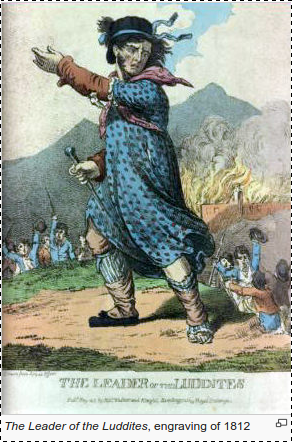
\includegraphics[width=0.2\textwidth]{figures/ludite_leader}}
\caption{The leader of the Ludites}
\label{title_page_1_ludites}
\end{figure}
 
%----------------------------------------------------------------------------------------

\vfill % Fill the rest of the page with whitespace

\end{titlepage} to your LaTeX file where you want your
% title page.
%
% In this example, we are using the 2nd method. You cannot compile this docuent by itself, since there is no '\begin|end{document}. You must compile the main document which calls this document.
%
%%%%%%%%%%%%%%%%%%%%%%%%%%%%%%%%%%%%%%%%%

%----------------------------------------------------------------------------------------
%	PACKAGES AND OTHER DOCUMENT CONFIGURATIONS
%----------------------------------------------------------------------------------------

%\documentclass[12pt]{article}
%
%\begin{document}

\begin{titlepage}

\newcommand{\HRule}{\rule{\linewidth}{0.5mm}} % Defines a new command for the horizontal lines, change thickness here

\center % Center everything on the page
 
%----------------------------------------------------------------------------------------
%	HEADING SECTIONS
%----------------------------------------------------------------------------------------
%
% The \\[metric] refers to the spacing after the text.
\textsc{\LARGE Linux System Administration}\\[1.5cm] % Name of your university/college
\textsc{\Large RHEL, CentOS, Fedora}\\[1.0cm] % Major heading such as course name
\textsc{\large Command Line Reference}\\[0.5cm] % Minor heading such as course title

%----------------------------------------------------------------------------------------
%	TITLE SECTION
%----------------------------------------------------------------------------------------

\HRule \\[0.4cm]
{ \huge \bfseries Linux System Administration}\footnote{This book is not intended for 19\textsuperscript{th} century textile workers or climate change deniers.}\\[0.4cm] % Title of your document
\HRule \\[1.5cm]
 
%----------------------------------------------------------------------------------------
%	AUTHOR SECTION
%----------------------------------------------------------------------------------------
%
% minipage is used when you want to place side by side two items, as in this case, or as in placing two pictures or tables side by side
%
\begin{minipage}{0.4\textwidth} % means .4 or 40% of textwidth, the width of the minipage
\begin{flushleft} \large
\emph{Author:}\\ % emph = emphasis or italics
Murray \textsc{davis} % Your name and \textsc = text_small_caps
\end{flushleft}
\end{minipage}
~
\begin{minipage}{0.4\textwidth}
\begin{flushright} \large
\emph{Topic:} \\
Linux \textsc{System Administration Version \versionnumber} 
\end{flushright}
\end{minipage}\\[4cm]

% If you don't want a supervisor, uncomment the two lines below and remove the section above
%\Large \emph{Author:}\\
%John \textsc{Smith}\\[3cm] % Your name

%----------------------------------------------------------------------------------------
%	DATE SECTION
%----------------------------------------------------------------------------------------

{\large \today{ - Compile Date } \textsl{November 3, 2016 - Revision Date}}\\[3cm] % Date, change the \today to a set date if you want to be precise

%----------------------------------------------------------------------------------------
%	LOGO SECTION
%----------------------------------------------------------------------------------------
%
% Note: The file is in the folder called figures that lies in the main directory. The file is called: cube.png, but you do not have to supply the filename extension '.png'.
%
\begin{figure}[!h]
\centering
\href{https://en.wikipedia.org/wiki/Luddite}{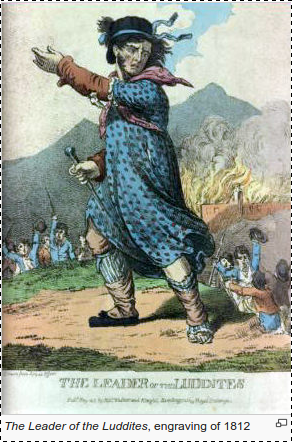
\includegraphics[width=0.2\textwidth]{figures/ludite_leader}}
\caption{The leader of the Ludites}
\label{title_page_1_ludites}
\end{figure}
 
%----------------------------------------------------------------------------------------

\vfill % Fill the rest of the page with whitespace

\end{titlepage} to your LaTeX file where you want your
% title page.
%
% In this example, we are using the 2nd method. You cannot compile this docuent by itself, since there is no '\begin|end{document}. You must compile the main document which calls this document.
%
%%%%%%%%%%%%%%%%%%%%%%%%%%%%%%%%%%%%%%%%%

%----------------------------------------------------------------------------------------
%	PACKAGES AND OTHER DOCUMENT CONFIGURATIONS
%----------------------------------------------------------------------------------------

%\documentclass[12pt]{article}
%
%\begin{document}

\begin{titlepage}

\newcommand{\HRule}{\rule{\linewidth}{0.5mm}} % Defines a new command for the horizontal lines, change thickness here

\center % Center everything on the page
 
%----------------------------------------------------------------------------------------
%	HEADING SECTIONS
%----------------------------------------------------------------------------------------
%
% The \\[metric] refers to the spacing after the text.
\textsc{\LARGE Linux System Administration}\\[1.5cm] % Name of your university/college
\textsc{\Large RHEL, CentOS, Fedora}\\[1.0cm] % Major heading such as course name
\textsc{\large Command Line Reference}\\[0.5cm] % Minor heading such as course title

%----------------------------------------------------------------------------------------
%	TITLE SECTION
%----------------------------------------------------------------------------------------

\HRule \\[0.4cm]
{ \huge \bfseries Linux System Administration}\footnote{This book is not intended for 19\textsuperscript{th} century textile workers or climate change deniers.}\\[0.4cm] % Title of your document
\HRule \\[1.5cm]
 
%----------------------------------------------------------------------------------------
%	AUTHOR SECTION
%----------------------------------------------------------------------------------------
%
% minipage is used when you want to place side by side two items, as in this case, or as in placing two pictures or tables side by side
%
\begin{minipage}{0.4\textwidth} % means .4 or 40% of textwidth, the width of the minipage
\begin{flushleft} \large
\emph{Author:}\\ % emph = emphasis or italics
Murray \textsc{davis} % Your name and \textsc = text_small_caps
\end{flushleft}
\end{minipage}
~
\begin{minipage}{0.4\textwidth}
\begin{flushright} \large
\emph{Topic:} \\
Linux \textsc{System Administration Version \versionnumber} 
\end{flushright}
\end{minipage}\\[4cm]

% If you don't want a supervisor, uncomment the two lines below and remove the section above
%\Large \emph{Author:}\\
%John \textsc{Smith}\\[3cm] % Your name

%----------------------------------------------------------------------------------------
%	DATE SECTION
%----------------------------------------------------------------------------------------

{\large \today{ - Compile Date } \textsl{November 3, 2016 - Revision Date}}\\[3cm] % Date, change the \today to a set date if you want to be precise

%----------------------------------------------------------------------------------------
%	LOGO SECTION
%----------------------------------------------------------------------------------------
%
% Note: The file is in the folder called figures that lies in the main directory. The file is called: cube.png, but you do not have to supply the filename extension '.png'.
%
\begin{figure}[!h]
\centering
\href{https://en.wikipedia.org/wiki/Luddite}{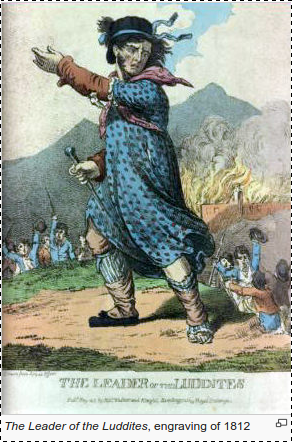
\includegraphics[width=0.2\textwidth]{figures/ludite_leader}}
\caption{The leader of the Ludites}
\label{title_page_1_ludites}
\end{figure}
 
%----------------------------------------------------------------------------------------

\vfill % Fill the rest of the page with whitespace

\end{titlepage} % downloaded template, note we do not have to specify '.tex' ending.

\pagestyle{plain}
% 
%
% tableofcontents is a command
%
% all lines beginning with '\chapter', '\section', 'subsection', etc.,  are complied/processed and a table of contents is created and placed where the line '\tableofcontents' appears in the 'main.tex' document. Everything is numbered automatically.
%
%
\setcounter{secnumdepth}{4} % how many sectioning levels to assign numbers to
\setcounter{tocdepth}{4}    % how many sectioning levels to show in ToC

\tableofcontents
%%%%%%%%%%%%%%%%%%%%%%%%%%%%%%%%%%%%%%%%%%%%%%%%%%%%%%%%%%%
%%%%%%%%%%%%%%%%%%%%%%%%%%%%%%%%%%%%%%%%%%%%%%%%%%%%%%%%%%%
%%%%%%%%%%%%%%%%%%%%%%%%%%%%%%%%%%%%%%%%%%%%%%%%%%%%%%%%%%%
%%
%% Note: instead of including each chapter inside the 'main.tex' document, we could create seperate files for each chapter. This would be useful if different persons worked on each chapter.
%%
%%
\chapter{Is ya 'ard at it all de time or wa?}
\label{ch:intro}
\pagestyle{fancy}

\fancyhf{} % here we clear any fancy header settings
%% Note, the first page of every chapter does not have a header.
\fancyhead[EC]{Linux System Administration}
\fancyhead[OC]{\leftmark} % O=odd pages, C= center, leftmark defaults to Chapter number and title
%\fancyhead[EC]{\rightmark} % E = even pages, C = center, rightmark defaults to number of current section
%%
%% Set, headheight to eliminate warning message "Package Fancyhdr Warning: \headheight is too small (12.0pt): Make it at least 13.59999pt.
\setlength{\headheight}{13.99pt} 
%%\setlength{\footheight}{13.6pt}
%%
% The next line would put a line at the bottom of every page starting from the second page of every chapter, if it was uncommented.
%%
%\renewcommand{\footrulewidth}{1pt}
%%
\cfoot{\thepage} % c = center, foot = footer, thepage = page number

\rhead{
\includegraphics[width=.5cm]{figures/smCanadianFlag}}
		
%%%%%%%%%%%%%%%%%%%%%%%%%%%%%%%%%%%%%%%%%%%%%%%%%%%%%%%%%%%
%%%%%%%%%%%%%%%%%%%%%%%%%%%%%%%%%%%%%%%%%%%%%%%%%%%%%%%%%%%

\section{License}

The documents in this GitHub repository will allow you to compile a LaTeX package of documents in order to generate a PDF document called main.pdf. However, if you are not interested in LaTeX, you can simply download and read the main.pdf document.

Copyright \textcopyright 2016 \author{Murray Davis} \href{mailto:iam@murraydavis.ca}{iam@murraydavis.ca}

This program is free software: you can redistribute it and/or modify
it under the terms of the GNU General Public License as published by
the Free Software Foundation, either version 3 of the License, or
(at your option) any later version.

This program is distributed in the hope that it will be useful,
but WITHOUT ANY WARRANTY; without even the implied warranty of
MERCHANTABILITY or FITNESS FOR A PARTICULAR PURPOSE.  See the
GNU General Public License for more details.

A copy of the \textsl{GNU\_General\_Public\_License.lic}, is included in the root folder of the source documents.  If you would like more information, see \href{http://www.gnu.org/licenses}{http://www.gnu.org/licenses/}.

\section{Contributing}

If you feel inclined to contribute to this book, please read the \textsl{CONTRIBUTING.md} document. By contributing, I mean any effort to improve the quality of the book. I have spent much time looking for coding errors, mistakes, poor grammar, mispellings, and other irritants. I would also entertain suggestions for future chapters or requests to clarify and improve upon content. The best way to offer suggestions is via the Issues function within this \keyword{github} project: \href{https://github.com/murraydavis/Linux-System-Administration}{https://github.com/murraydavis/Linux-System-Administration}.

\section{Newfinese}

Whatta ya at? What are you doing? Newfies, who live on the island of Newfoundland, Canada have a unique and rich vocabulary, some may even say they have their own language. If you are up for a linguistic challenge, offer to pay for a night of drinking at a local pub favoured by the Newfoundland diaspora. Your head will swirl with incomprehensible speech, wild stories, and the intoxication of living life to its fullest. This chapter title can roughly be translated as, "Are you working hard all the time or what?"

\section{Free as in beer}

This book is a gift to the open source Linux community. I have received so much from Internet-based authors who have shared their knowledge and expertise. I hope that my book will in a similar way help further the learning of those who choose Linux over \emph{Micro\$loth} and who also wish to embrace the open source concept. However, I do request that each reader put in a fair amount of effort and hard work experimenting with and testing my code and examples. If you feel obligated in some way, I suggest you also try to share with others your nuggets of gold and good fortune. Or, why not donate time, energy, or money to a worthy cause? Here is a short URL list of my favourite charities. 

\begin{enumerate}
	\item{\href{http://cpawsbc.org/}{Canadian Parks and Wilderness Society}}
	\item{\href{http://www.msf.ca/}{Medicin Sans Frontiers}}
	\item{\href{https://playingforchange.com/}{Playing for Change}}
\end{enumerate}

\section{Women, STEM, coding, IT careers}

The women with whom I have worked in IT have had incredible skill and ability. Nothing gets done well unless you work as a team and women embrace team spirit innately. \textit{I think we should encourage girls and young women to pursue careers in \href{http://www.stemeducationawareness.ca/canadian-innovation/challenging-the-barriers-between-girls-and-stem}{STEM}}. Here is a short list of organizations that encourage women to participate in coding and IT careers.

\begin{enumerate}
	\item{\href{http://geekfeminism.wikia.com/wiki/Geek_Feminism_Wiki}{Geek Feminism}}	
	\item{\href{http://adainitiative.org/}{Ada Initiative}}
	\item{\href{https://www.gnome.org/outreachy/}{Outreachy}}
	\item{\href{http://ladieslearningcode.com/girlscodeday/}{Ladies Learning Code}}
	\item{\href{https://www.womenwhocode.com/}{Women Who Code}}
\end{enumerate}

\section{Omnist Eggs}

Yes, there are a few.

\section{\latex}

This document was written using \latex, a high quality typesetting system. I did most of my work on two home PCs, one had the \tbi{Fedora 23} operating system, the other was a Macbook Pro with the \tbi{El Capitan} operating system. On both systems, I installed the full \latex package. With Fedora, the command I used was \emph{sudo dnf install texlive-scheme-full}. This is a lot of overkill, but I wanted to be sure that I had all texlive packages. The drawback is that when updates are available for texlive, you need to go for a long run or tip a few beers while the update is happening. \textit{I recommend that you just install the base \emph{texlive} package and then install extra packages as needed}.

Here is a short URL list of \latex resources...

\begin{enumerate}
	\item{\href{https://www.ctan.org/}{CTAN: The Comprehensive \tex Archive Network}}
	\item{\href{https://tex.stackexchange.com/}{Stackexchange's \tex}}
	\item{\href{https://www.tug.org/}{\tex Users Group}}
	\item{\href{https://www.latex-project.org/}{The \latex Project}}
	\item{\href{https://en.wikibooks.org/wiki/LaTeX}{\latex WikiBooks}}
	\item{\href{http://www.dickimaw-books.com/latexresources.html}{Dickimaw Books \latex}}
	\item{\href{http://mirror.its.dal.ca/ctan/info/lshort/english/}{The Not So Short Introduction to \latex\begin{math}2\epsilon\end{math}}}
	\item{\href{https://www.youtube.com/watch?v=Qjp-a2uZWZc}{\latex Basic Elements for writing a book/thesis}}
\end{enumerate}

The structure of my book is based on \tbi{Mauricio Lobos'} excellent documentation and Youtube video, the last link in the above list. \textit{If you want to learn an organized approach to writing a \latex book watch his video and study his code.} Mauricio, many thanks!

Since I needed to display a lot of \emph{Linux bash code}, I initially relied on two \latex packages that help typeset code (follow these links): \href{https://www.ctan.org/pkg/listings?lang=en}{listings} and  \href{https://www.ctan.org/tex-archive/macros/latex/contrib/minted?lang=en}{minted}. 

I switched back and forth between these two packages when I started working on the book. The reason for this inconsistency was that neither package seemed to provide all the typesetting features that I wanted to implement. Therefore, depending on the task, I chose the package that implemented the desired typesetting feature for the chunk of code that I was working on.

I also found that I needed version 2.1 of \emph{minted} because it supported the [breaklines] option. The default Fedora 23 \latex version 1.7 did not support [breaklines]. I manually installed the newer version and then I created an alias for my updates: \emph{alias yu = dnf update -x texlive-minted}. Thus, when I wanted to update the Fedora packages, I simply issued my alias command \emph{yu} and the update process excluded the \emph{texlive-minted} package during the update. Without this alias override, the \emph{dnf -update} would actually downgrade and replace my 2.1 version with the 1.7 version.\\

If you wanted to use version 2.1 of minted, download the minted package using the above \emph{minted} link and extract it. Next, delete this folder: \textsl{/usr/share/texlive/texmf-dist/tex/latex/minted} . Do not simply copy/replace. Delete the folder first and then copy the extracted minted package to that folder. You then have to refresh texlive by issuing this command \emph{sudo texhash}. As well, you must add the \emph{-{}-{}shell-escape} option to all \tex compilation commands. I used the \emph{TeXstudio} package while writing this book. Here is a screenshot of my \emph{TeXstudio} configuration for the commands used to compile my documents.

% Show diffirences between default \todo and color todos defined in packages.tex
%\todo[inline]{Create a chapter illustrating the differences between minted and lstlisting.}

\begin{figure}[!h]
\centering
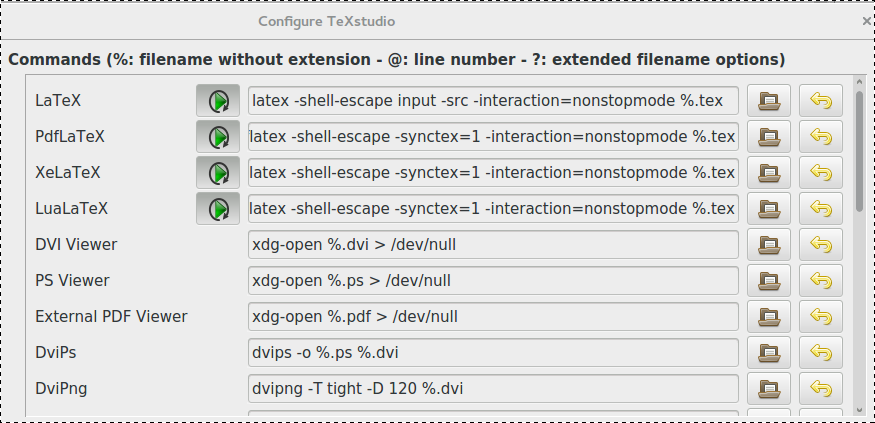
\includegraphics[width=0.75\textwidth]{figures/TeXstudio}
\caption{Configure \tex{}studio}
\label{ch_1_texstudio_config}
\end{figure}

%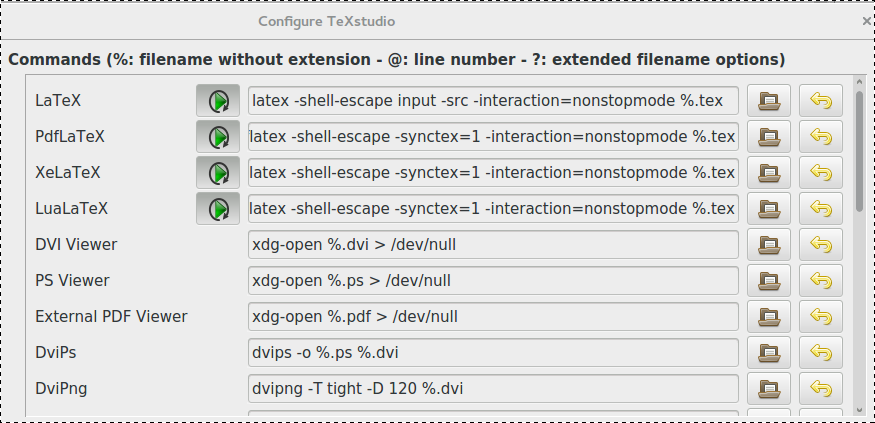
\includegraphics[width=0.75\textwidth]{figures/TeXstudio}

If you are interested in using \latex to display \emph{bash} code, take a look at the \emph{packages.tex} document in the \textsl{settings} folder of the source documents on my \emph{GitHub} site. In the \emph{packages.tex} document there is a \emph{\textbackslash{}lset\{\}} block of code.\footnote{I apologize to the author but I do not recall where I found the block of code.} It is this code that formats the \emph{lstlisting} package that displays the \emph{bash} code. It was this code that allowed me to dispense with the \emph{minted} package.

\add{Add a chapter illustrating the differences between minted and lstlisting.}

\section{\latex and dynamic links}

Since this document is typeset using \latex, you will find many hyperlinks embedded through out the document. I try to clearly identify hyperlinks, but the only true indication that text is a hyperlink is when you hover the mouse over text that is colored, the mouse icon changes from a pointer to a small hand. The hyperlink may be to an external source such as an Internet Webpage or the hyperlink may be to another part of the document.

\section{Where's the meat and potatoes?}

If you don't like reading code, you may not find this book all that appetising. I use lots of comments in my code. In a way, the \emph{comments} are the \emph{Meat and Potatoes}. You will also see that I am a big fan of manpages. I consider the manpages as the \emph{gravy}. I am sure that I will annoy you with my repeated attempts to encourage you to read manpages. Actually, the manpages are just a subset of the documentation that is available to help you learn about Linux commands. \textit{You will not get your \emph{dessert} unless you read the documentation!}

\section{Punctuation} 

Writing about code presents several challenges to the goal of writing with clarity. For example, some Linux commands can be used as verbs. How should one distinguish between the regular use of the command and the verb use of the command? I have chosen the following conventions:

\begin{itemize}
	\item \tbi{Double quotations ""} I surround string names with the double quotation.
	\item \tbi{Single upright quotation \textquotesingle{}\textquotesingle{}} I use single upright quotations to highlight commands with command options. Alternatively, I sometimes place a command with options unquoted after a colon.
	\item \tbi{\emph{Emphasis}}  I use \emph{emphasis} to highlight Linux commands, software names, usernames, etc.
	\item \tbi{Lists of commands} If I list several commands in a row after a colon, I will not put use emphasis.
	\item \tbi {Bold-italic} To highlight a command, I sometimes use bold-italic.
	\item \tbi{Italics} If I have a suggestion for you, if I recommend that you test something, I will put the recommendation in \textit{italics}.
	\item \tbi{Caps} Technical terms that are ubiquitous and always written in caps are left in caps, unless I choose to put them in bold-italic for emphasis.
	\item \tbi{Slanted text} I use slanted text for pathnames \textsl{/home/myhome/myfolder}.
	\item \tbi{Keywords} I use the \latex \keyword{keyword} font to highlight \emph{keywords} such as a command like \keyword{mkdir}. I then build an index of the keywords that are listed at the end of this book.
\end{itemize}

\section{Who do you think you are?}

As per the little flag in the header of this document, I am proudly Canadian-eh. After high-school, without the high, I toiled purposely and industriously at University. Upon graduation, I worked on the high seas of accountancy\footnote{\href{https://www.youtube.com/watch?v=7YUiBBltOg4}{Monty Python's Meaning of Life}}, moved on to being a cultured madman\footnote{\href{http://www.penguin.com/static/html/classics/readingguides/deptfordtrilogy.php}{RobertsonDavies - Deptford Trilogy}}, and then finally careened towards IT. I have expired certifications in: A+, Microsloth MCSE 2000/2003, Cisco CCNP, CIISP, and GSEC.

I began my IT career working for a small IT consulting company. For 2 years, I did everything from laying CAT 5 wiring and setting up LANs to hosting websites and email on a FreeBSD server. This is when I began working with Linux. Next, I worked for a large oil-field services company as a Senior Systems Analyst contributing to environmental degradation and global warming. I spent most of my time with Cisco and other network vendor's gear managing LANs within the company's WAN. Guilt about my role in contributing to the slow death of our planet began to override my drive for financial gain and I chose to find alternate employ. For the past several years, I have worked again as a Senior Systems Analyst, this time for a manufacturer of energy saving products supporting a mixed Microsoft-Linux environment.

In my spare time, I read British and Canadian history, paddle a SUP, run long distances, cycle (and re-cycle), and ballroom dance with my wife. As you will notice, I use the metric system\footnote{\href{http://www.joeydevilla.com/2008/08/13/countries-that-dont-use-the-metric-system/}{Metric makes sense unless you have twelve fingers.}}, the British spelling system (unless typesetting \latex and creating man pages), and the Oxford and.

One of my favourite quotes that I think adequately sums up the human condition is the following: \tbi{Time flies like an arrow, fruit flies like a banana.}

\section{More context}

The type of Linux support that I provide at work is fairly limited. Here is a not-complete list of the type of Linux-related tasks that I work on...

\begin{itemize}
	\item \tbi{Building virtual servers for the user community: } I get requests from various departments to build specific-purpose Linux servers. I build the servers on an open source host. The Linux flavour depends on user preference. Some users like Ubuntu, some Debian, some Centos, some Fedora.
	\item \tbi{Building and managing virtual servers for System Administration: } Our DNS, SQL, internal web, and network monitoring servers are Linux-based.
	\item \tbi{Supporting manufacturing team: }The manufacturing team use Linux workstations in various stages of the manufacturing process. The tools are fairly sophisticated and run only on Linux.
	\item \tbi{Supporting Linux users: } Linux users tend to be fairly independent and able, so the type of support tends to be at a higher level than basic support. I typically deal with issues related to: setting up Samba shares, Git connections to software repositories, setting up Virtual Machines, SSH connectivity, permissions and ACLs, Apache and Wordpress configurations, Linux package configurations, etc.
\end{itemize}

As previously stated, at home, I alternate between using a Fedora 23 box and a MacBook Pro laptop, depending upon where I want to work. If it is warm and sunny on the deck and the beer is cold, I have no choice but to use the MBP laptop. With the Fedora 23 box, my home folder is on a separate partition from the root drive. On an irregular basis, I backup my home folder with rsync (a manual process). Occasionally, I shut my system down and use \href{http://clonezilla.org/downloads.php}{Clonezilla} to image my hard drive to a second hard drive. I have been able to mostly ween myself from the Microsoft bosom. The exceptions are few and are all related to software vendors who refuse to provide a Linux alternative. In order to deal with these exceptions, I built a couple of Windoze VMs using \href{http://virt-manager.ort}{Virtual Machine Manager} and launch these whenever I have to use the proprietary software...which thankfully is rarely.

\section{What's it all about Murray?}
\label{sec:allabout}

This book is principally about one thing: working at the command line using Linux builtin commands and \href{http://www.gnu.org/software/coreutils/coreutils.html}{GNU Coreutils}. If you become proficient at the command line, you will have mastered an important piece of becoming a Linux System Administrator. Since, I wrote this book using the \latex typesetting system, the title has become: \tbi{Writing about Linux System Administration using \latex}.

Like most things, the more you dig into them and play around, the more you learn. I am a proponent of \tbi{RTFM}\textit{\tbi{ - Read The Funky Manual} and don't think that someone will simply give you all the answers to your questions so that you don't have to expend any effort at all}.

This book has a very exploratory approach. You will find that I present code in a step-by-step manner supported by a lot of comments. I issue a command and maybe it doesn't work. I then try another command. Along the way, I attempt to describe my reasoning and methodology.

\tbi{Disclaimer:}

\begin{addmargin}[1em]{2em}
\textit{I am very old. I have a lot of memories, clutter, and useless pieces of information stuck between my ears. I simply cannot retain all the diverse bits of code and jetsam that are in my brain that I find useful. Just a sec, is it my brain that is useful or are the bits of information useful? Better get rid of the danglies\footnote{\href{http://blog.oxforddictionaries.com/2011/09/participles-how-not-to-dangle/}{Oxford Dictionaries to the rescue}} and rewrite this sentence. I simply cannot retain all the useful and diverse bits of code and jetsam that clutter the inside of my brain.}
\end{addmargin}

In order to address this issue of running out of brain disk space, I began documenting my Linux System Administration adventures using notebooks and binders and simple digital text documents. Much later, I switched to using \href{https://evernote.com}{Evernote}. Evernote is fairly useful for brain dumping information and creating folder hierarchy, but it is a pain to search and organize your information. Evernote refuses to create a Linux package for its product.\footnote{\href{https://www.youtube.com/watch?v=eGKdle1bbvo}{The company should also feel shame.}} However, there is a pretty good Linux alternative called \href{http://sourceforge.net/projects/nevernote/}{NixNote} which is what I use on my Fedora 23 system. For some reason, I cannot copy a webpage clip into NixNote. I can copy it as unformatted text, but if I try to copy it directly, I get a sync error. Instead, I have to use Evernote's Web Client in order to copy a webpage into my Evernote repository. I can then sync this cloud version of Evernote from the NixNote client.

Consequently, I wanted to move my notes from Evernote to a digital book form that had these features: indexing, table of contents, a professional look, sophisticated search capability, ease of revision, and a well-supported open source community behind it. Enter \latex! What a wonderful adventure this has been! Not only am I sharpening my Linux skills, but in the process I am developing a new skill, typesetting with \latex. My first motivation to use \latex came when I started a couple of \href{https://en.wikipedia.org/wiki/Massive\_open\_online\_course}{MOOCs}. The first was Coursera's \href{https://www.coursera.org/course/scicomp}{High Performance Scientific Computing} offered by the University of Washington's \href{http://faculty.washington.edu/rjl/}{Dr. Randall J. LeVeque}. \textit{If you want to improve your understanding of Linux and Python and you like math, take this course.} The other course was an EdX course,  \href{https://www.edx.org/course/introduction-solar-systems-astronomy-asux-ast111x-0}{Introduction to Solar Systems Astronomy}. I audited both courses. To help in retaining content, I wanted ready access to my notes, comments, and explorations that were typeset, especially important with the EdX course since it used many complex differential equations. This is where LaTeX excels...typesetting scientific and mathematical formulae.

And, finally, one topic that Dr. LeVeque covered in the HPSC course was \href{https://github.com/}{GitHub}.  Dr. LeVeque's discussions on \keyword{GitHub} helped me position this book as a collaborative project so that others can download it and contribute to its improvement.

I started this book in the early winter 2015 and finished the first published version in the fall of 2016.

\section{What this book is not about!}

This book is not a brain dump that can be used to easily challenge the current Linux certification exams. The book may help you get a base understanding of Linux System Administration tasks, but your study or reading of this book will not on its own help you succeed in passing these exams. In fact, when you check the curriculum for each certification, you will see that there are many gaps in the knowledge base that I present in this book. Here is a URL list of the main organizations that provide Linux certifications.

\begin{enumerate}
\item{\href{https://training.linuxfoundation.org/certification/lfcs}{Linux Foundation Certified System Administrator}}
\item{\href{https://www.lpi.org/certification/}{Linux Professional Institute}}
\item{\href{https://www.redhat.com/en/services/certification}{Red Hat Certification}}
\end{enumerate}

\section{\href{http://www.poetryfoundation.org/poem/171647}{Beware the Jabberwok, my son!}}

\textit{Trust nothing that I have written! Find alternative explanations! Verify everything and test all commands! Do not simply memorize a command, make sure it works.} This warning is especially applicable to non-Fedora-system users. Will the commands that I present work on a Debian or BSD system? The code will more likely work best on Fedora, CentOS, and RHEL systems.

My style of writing and the quality of my writing will undoubtedly displease some, cause bad gas and foul odours, but so be it. This book on Linux System Administration is a compilation of my investigation to understand the  Linux command line. Each time I check and edit my notes, I seem to come across syntax and coding errors and discover further insights. I have endeavoured to present code and information that is error free, but there is no guarantee that I have eliminated all errururs. I encourage you to point out errors and to make suggestions. If you only want to heap scorn on me, censure me, and build a wall of unkindness, I suggest that you join a political party that aligns with your sensibilities.\\

This book may become a living document for the next couple of years as long as my energies and interest remain high, that is, as long as red wine remains affordable and beer remains cold.

\howto{Latex - How to make list of all URLs?}






\chapter{An Important Chapter}
\label{ch:impch}
\pagestyle{fancy}

\fancyhf{} % here we clear any fancy header settings
%% Note, the first page of every chapter does not have a header.
\fancyhead[EC]{Linux System Administration}
\fancyhead[OC]{\leftmark} % O=odd pages, C= center, leftmark defaults to Chapter number and title
%\fancyhead[EC]{\rightmark} % E = even pages, C = center, rightmark defaults to number of current section
%%
%% Set, headheight to eliminate warning message "Package Fancyhdr Warning: \headheight is too small (12.0pt): Make it at least 13.59999pt.
\setlength{\headheight}{13.99pt} 
%%
% The next line would put a line at the bottom of every page starting from the second page of every chapter, if it was uncommented.
%%
%\renewcommand{\footrulewidth}{1pt}
%%
\cfoot{\thepage} % c = center, foot = footer, thepage = page number
\rhead{
\includegraphics[width=.5cm]{figures/smCanadianFlag}}
		
%%%%%%%%%%%%%%%%%%%%%%%%%%%%%%%%%%%%%%%%%%%%%%%%%%%%%%%%%%%
%%%%%%%%%%%%%%%%%%%%%%%%%%%%%%%%%%%%%%%%%%%%%%%%%%%%%%%%%%%

\section{Introduction}

\textit{Please spend time reading and studying this chapter and the next chapter on programming.} If you do, the rest of the book will be much easier to understand and you will have a firm understanding of the Linux command line. The chapters on the manpage and profiles are also essential reading.

The way that I have ordered the presentation of the material may frustrate some, yet bore others. \textit{But, do continue reading as some of your confusion may be addressed in subsequent chapters.} There may be even the odd pearl for the more advanced users.

I cannot stress (actually, I will continually stress) how important it is to read manpages and other online documentation. \textit{But, don't just read the documentation, test the code and syntax, run the examples, and play with the command options.} As Cole Porter wrote, \tbi{\textcolor{red}{\href{https://www.youtube.com/watch?v=slYExz44k0Q}{Experiment!}}}\footnote{Kevin Klein's version from the movie De-Lovely}

\section{Resources}

If you are bored and totally fed up with reading this book, you can lose hours of your finite time on this planet looking at the following web sites. Some are fairly clean with little annoying flotsam and jetsam. No, not that early 80's Thrash Metal band from Phoenix, I am referring to Internet advertising or web advertising. But, in the end, everyone has to make a living...

\begin{enumerate}
	\item{\href{http://tldp.org}{The Linux Documentation Project}} 
		A little dated but still relevant: HOWTOs, Guides, FAQs, manpages, Advanced Bash-Scripting Guide
	\item{\href{https://www.gnu.org/doc/doc.en.html}{Documentation of the GNU Project - GNU Manuals}}
	\item{\href{https://www.linux.com/tutorials}{Linux.com - News for the Open Source Professional - Tutorials}}
	\item{\href{https://www.howtoforge.com/}{Linux Tutorials}} 
		Trust me, you will often visit this site!
	\item{\href{http://stackoverflow.com}{Linux documentation and forums}} 
		Stock Overflow is the largest online community for programmers to learn, share their knowledge, and advance their careers.
	\item{\href{http://fedoralinuxcommands.blogspot.ca/}{Alphabetical listing of linux commands}} 
	\item{\href{http://unix.stackexchange.com/}{Unix \& Linux}} 
		A question and answer site for users of Linux, FreeBSD and other Un*x-like operating systems.
	\item{\href{https://access.redhat.com/documentation/en/}{Product documentation for redhat}} 
		And thus besides documentation for RHEL, documentation that is relevant to CentOS and Fedora...and other Linux OS.
	\item{\href{http://www.linuxquestions.org}{A site for asking and answering questions about Linux}}
	\item{\href{http://www.unix.com}{unix and linux operating commands}} 
		A forum for for programmers and operating specific Linux OS.
	\item{\href{https://debian-handbook.info/}{The Debian Administrator's Handbook}} 
\end{enumerate}

\section{\color{red}Copy/paste of code...optional to read.}

This section is indeed optional. \textit{If you want to learn a bit about typesetting \latex and the \keyword{lstlisting} package, read this section.}

As I have indicated in the previous chapter, I used the \latex \keyword{lstlisting} package to typeset the \emph{bash} code. However, there was one issue that initially stumped me. The issue was that \latex converted the \keyword{minus} sign to an \keyword{emdash} when it compiled the source code to produce the final \keyword{PDF} document. To create the bash code in the source documents, I simply copied from the command line and pasted into my \latex source documents, the \emph{.tex} files. Why was the \emph{empdash} an issue? Well, when you copied a command from the bash code sections of the PDF book to the command line, the command would fail, \textit{if the command contained minus signs now typeset as an emdash.} The bash terminal would balk at the \emph{emdash}, it did not know how to interpret the \emph{empdash}. I initially devised a work around. You will learn some coding by reading this section. You will also see the process of how this document evolved...as I was addressing both \latex and \keyword{Linux} coding issues.

\lstset{
	keywords={tar,gzip},
	rulecolor=,
	language=bash,
	basicstyle=\small,
	upquote=true,
	aboveskip={1.5\baselineskip},
	showstringspaces=false,
	extendedchars=true,
	breaklines=true,
	prebreak = \raisebox{0ex}[0ex][0ex]{\ensuremath{\hookleftarrow}},
	frame=single,
	showtabs=false,
	showspaces=false,
	showstringspaces=false,
	identifierstyle=\ttfamily,
	keywordstyle=\color[rgb]{0,0,1},
	commentstyle=\color[rgb]{0.133,0.545,0.133}\fontseries{lc}\selectfont\itshape,columns=fullflexible,
	stringstyle=\color[rgb]{0.627,0.126,0.941}
}

In the next section of code, you will see the difference between the \keyword{hyphen} and the \keyword{emdash}. Look carefully! There is only a subtle difference in the length of these two characters. In typsetting there are three basic forms used for hyphenation: hyphen (minus sign), endash(about the width of the letter n), and emdash (about the width of the letter m). So, in terms of length, we work from right to left, with the \emph{hyphen} as the shortest and the \emph{emdash} as the longest. As well, I am going to use the words \emph{hyphen} and \emph{minus sign} interchangeably, but they both are words for the shortest form of hyphenation.

\begin{lstlisting}[escapeinside={¿}{¿},frame=single,breaklines]
#
# Here is a typical line of code. Copy and paste it into your terminal window from this block of code. The command looks for all files that do not have either a .txt or .cfg file extension. At this point, it is not necessary that you understand each component of the command. Also, please note taht file name expansion works with either the double parentheses or the single paranthesis. I use the former in the following examples.
#
¿\tld¿ find . -type f ! \( -name "*.txt" -o -name "*.cfg" \)
#
# Did you get the following error message when you tried to execute the command?
#
find: paths must precede expression: -name
Usage: find [-H] [-L] [-P] [-Olevel] [-D help|tree|search|stat|rates|opt|exec] [path...] [expression]
#
# What about this command?
#
¿\tld¿ ls -la
ls: cannot access -la: No such file or directory
\end{lstlisting}

So, the error message will vary depending on what follows the first \emph{emdash}. Well, that would be a pain in the ass to have to edit every command that you wanted to try. You would edit the command inline, deleting the \emph{emdash} and retyping a hypen. \keyword{Linux System Administration} to your rescue! I am going to show you right off the top how knowledge of scripting and troubleshooting can fix some very vexing and strange issues. To solve this issue, I am going to use \keyword{sed}, a Linux command that is used to process strings.

\begin{lstlisting}[escapeinside={¿}{¿},frame=single,breaklines]
#
# First of all, we need to replace the emdash with a normal minus sign. You can copy and paste these commands to your command line because I have used the power of ¿\color[rgb]{0.133,0.545,0.133}\latex¿ to properly format them for the command line.  I am sending a string to sed and the string is the complex find command inside the double parentheses.
#
¿\tld¿ sed s/-/¿{-}¿/ <<< "find . -type f ! \( -name "*.txt" -o -name "*.cfg" \)"
find . ¿{-}¿type f ! \( -name *.txt -o -name *.cfg \)
#
# Note, look closely, only the first minus sign after find . is a true minus sign. Our command only replaced the first instance. We have to modify it slightly and say replace all instances using sed's global option.
#
¿\tld¿ sed s/-/¿{-}¿/g <<< "find . -type f ! \( -name "*.txt" -o -name "*.cfg" \)"
find . ¿{-}¿type f ! \( ¿{-}¿name *.txt ¿{-}¿o ¿{-}¿name *.cfg \)
#
# We now copy the output and type it on a new command line and hit enter. There actually is a much easier way to do this than copy and pasting that I will show in a later section of this book. I only show a truncated list of such files on my system.
#
¿\tld¿ find . ¿{-}¿type f ! \( ¿{-}¿name *.txt ¿{-}¿o ¿{-}¿name *.cfg \)
./my.dbl
./gl.err
.
.
./statinode.sh.old
./vic.sh
#
# Well, that would be a pain in the ass to have to do each time! Fortunately, we can pass the output immediately to the shell using a process called "here stringing", the three less than symbols; and piping to the shell, |  sh 
#
¿\tld¿ sed s/-/¿{-}¿/g <<< "find . -type f ! \( -name "*.txt" -o -name "*.cfg" \)" | sh
./my.dbl
./gl.err
.
.
./statinode.sh.old
./vic.sh
#
# That's still a labour intensive process. We need a script to automate the process. $1 represents the command that we are going to pass to our script.
#
¿\tld¿ cat emdash.sh
¿\tbi{\#}¿!/bin/bash
sed s/-/¿{-}¿/g <<< "$1" | sh
#
# We first make our script executable...explained in a later section.
#
¿\tld¿ chmod u+x emdash.sh
#
# We can now pass the command that we copied from my book to the command line after ./emdash.sh
#
¿\tld¿ ./emdash.sh find . -type f ! \( -name "*.txt" -o -name "*.cfg" \)
./my.dbl
./gl.err
.
.
./statinode.sh.old
./vic.sh
\end{lstlisting}

With my initial solution, if you wanted to run any command taken from a block of code, you needed to convert those \emph{minus signs}. If you want to search this typesetting issue further play around with the \keyword{asterix}. In the \latex code, you will see that the \emph{asterix} is a superscript, but in the PDF document, the \emph{asterix} is a subscript. You could also have an issue with this if you were copying from the PDF document to the command line and then back from the command line to the \latex code.

So, as an author, I had a couple of options. I could change all \emph{emdashes} in my book to true minus signs, so that all copy and pastes worked for the reader. For users who want to compile my \latex code, that would put an unusual amount of strain on their systems because the \latex compiler would have to convert this code {?`}{\{-}\}{?`} to {-}. I would, of course, first have to go through my entire document and replace each emdash -- with {?`}{\{-}\}{?`}. Ugh!

Another alternative was to create a simple table after each code block that would summarise essential commands. Readers could then copy and paste from the table.

\subsection{Solution to \latex \keyword{emdash} and \keyword{minus sign}}

I finally found the \latex \emph{lstlisting} typsetting instruction that resulted in an \emph{hyphen/minus} sign appearing as an \emph{emdash}.  The \emph{basicstyle=small} setting that I had defined for the \keyword{lstlisting} package in the \textsl{settings/package.tex} file had to be changed.

\begin{lstlisting}[escapeinside={¿}{¿},frame=single,breaklines]
\lstset{
	keywords={tar,gzip},
	rulecolor=,
	language=bash,
	basicstyle=small,
	upquote=true,
	aboveskip={1.5\baselineskip},
	showstringspaces=false,
	extendedchars=true,
	breaklines=true,
	prebreak = \raisebox{0ex}[0ex][0ex]{\ensuremath{\hookleftarrow}},
	frame=single,
	showtabs=false,
	showspaces=false,
	showstringspaces=false,
	identifierstyle=\ttfamily,
	keywordstyle=\color[rgb]{0,0,1},
	commentstyle=\color[rgb]{0.133,0.545,0.133}\fontseries{lc}\selectfont\itshape,columns=fullflexible,
	stringstyle=\color[rgb]{0.627,0.126,0.941},
}
\end{lstlisting}

I had to change that line to \emph{basicstyle=ttfamily}. I then recompiled my \latex code and now my \emph{minus signs} appeared as a true \emph{minus sign}. I could now copy from my PDF's bash code sections to the command prompt and the lines would execute properly. 

However, I still had an issue with copying commands that extended beyond the width of the page. I could not copy those lines because the command line would try to interpret the left arrow sign at the page break.

\lstset{
	keywords={tar,gzip},
	rulecolor=,
	language=bash,
	%basicstyle=\scriptsize,
	basicstyle=\ttfamily,
	upquote=true,
	aboveskip={1.5\baselineskip},
	showstringspaces=false,
	extendedchars=true,
	breaklines=true,
	prebreak = \raisebox{0ex}[0ex][0ex]{\ensuremath{\hookleftarrow}},
	%prebreak={},
	frame=single,
	showtabs=false,
	showspaces=false,
	showstringspaces=false,
	identifierstyle=\ttfamily,
	keywordstyle=\color[rgb]{0,0,1},
	commentstyle=\color[rgb]{0.133,0.545,0.133}\fontseries{lc}\selectfont\itshape,columns=fullflexible,
	stringstyle=\color[rgb]{0.627,0.126,0.941}
}

\begin{lstlisting}[escapeinside={¿}{¿},frame=single,breaklines]
#
# Try copying this line to your command prompt. Notice, the left arrow at the end of the first line. The command looks for all files with spaces in their names and replaces the space with an underscore.
#
[~] find . -depth -name '* *' -exec sh -c 'D=$(dirname "$0"); F=$(basename "$0"); mv "$0" "$D/${F// /_}"' '{}' \;
#
# At the command prompt, you line will appear as...
#
find . -depth -name '* *' -exec sh -c 'D=$(dirname "$0"); F=$(basename "$0");¿$\leftarrow$¿-
> mv "$0" "$D/${F// /_}"' '{}' \;
#
# Hit the enter key after the second line and you will get a command not found error. There was one file in the current directory called: a b.txt, the file name has a space between the a and b.
#
./a b.txt: ¿$\leftarrow$¿-: command not found
\end{lstlisting}

\subsection{Solution to visible prebreak symbol}

Fortunately, the solution was also simple. I just needed to change the \keyword{prebreak} setting for the \emph{lstlisting} package to an empty setting.

\lstset{
	keywords={tar,gzip},
	rulecolor=,
	language=bash,
	basicstyle=\ttfamily,
	upquote=true,
	aboveskip={1.5\baselineskip},
	showstringspaces=false,
	extendedchars=true,
	breaklines=true,
	prebreak={},
	frame=single,
	showtabs=false,
	showspaces=false,
	showstringspaces=false,
	identifierstyle=\ttfamily,
	keywordstyle=\color[rgb]{0,0,1},
	commentstyle=\color[rgb]{0.133,0.545,0.133}\fontseries{lc}\selectfont\itshape,columns=fullflexible,
	stringstyle=\color[rgb]{0.627,0.126,0.941}
}

\begin{lstlisting}[escapeinside={¿}{¿},frame=single,breaklines]
#
# Try copying this line to your command prompt. 
#
¿\tld¿ find . -depth -name '* *' -exec sh -c 'D=$(dirname "$0"); F=$(basename "$0"); mv "$0" "$D/${F// /_}"' '{}' \;
#
# The command will complete successfully, but you will notice that on the second line after the split there will be a greater than symbol, which the shell will ignore in executing the command. Your command appears as follows with the blinking cursor at the end of the second line. Just hit enter key and the command will execute.
# 
¿\tld¿ find . -depth -name '* *' -exec sh -c 'D=$(dirname "$0"); F=$(basename "$0"); 
> mv "$0" "$D/${F// /_}"' '{}' \;
#
# The execution of the command replaces the space in any file name with spaces with an underscore: a b.txt to a_b.txt.
#
\end{lstlisting}

\subsection{Final settings for \latex \emph{lstlisting} package.}
	
Our final settings for the typsetting of the \emph{lstlisting} package as defined in \textsl{settings/packages.tex}.

\begin{lstlisting}[escapeinside={¿}{¿},frame=single,breaklines]
\lstset{
keywords={tar,gzip},
rulecolor=,
language=bash,
¿\color{red}basicstyle=\textbackslash{}ttfamily¿,
upquote=true,
aboveskip={1.5\baselineskip},
showstringspaces=false,
extendedchars=true,
breaklines=true,
¿\color{red}prebreak=\{\}¿,
frame=single,
showtabs=false,
showspaces=false,
showstringspaces=false,
identifierstyle=\ttfamily,
keywordstyle=\color[rgb]{0,0,1},
commentstyle=\color[rgb]{0.133,0.545,0.133}\fontseries{lc}\selectfont\itshape,columns=fullflexible,
stringstyle=\color[rgb]{0.627,0.126,0.941}
}
#
# There are 3 more lstlisting settings that are set at the beginning of each block of code throughout the book.
#
¿\textbackslash{}begin\{lstlisting\}[escapeinside=\{?`\}\{?`\},frame=single,breaklines]¿
***
***Code goes here***
***
¿\textbackslash{}end\{lstlisting\}¿
\end{lstlisting}

The frame setting puts a box around the code. The escape inside character is needed to escape back to \latex, so that \latex commands can typeset within the block of code. The breaklines setting is actually redundant since it is already defined in \textsl{settings/package.tex} \emph{lstset}.

\change{Remove \emph{lstlisting} settings at each block of code and to \textsl{settings/package.tex} \emph{lstset}}.

\subsection{Building an index - a two compile process}

When you complile the \latex document, you need to build an index. As mentioned, I used TeXstudio to write and compile my document. Compiling is a three step process. These steps can also be accomplished at the command line...just search the \latex compile process using Google.

\begin{enumerate}
	\item{Compile the document. Click the green compile arrow or press F6.}
	\item{Index the document. Click Tools/User/1. Make Nomenclature or press Alt-Shift-F1.}
	\item{Compile the document.}
\end{enumerate}

\keyword{Make Nomenclature} is a User Command. Click Options/Configure TeXstudio and then choose the Build menu on the left-hand side. Scroll to User Command. I called the command: Make Nomenclature. The command is: \textsl{makeindex -t \%.nlg -o \%.nls \%.nlo}. Unfortunately, I cannot reference the source of this command that I found somewhere on the Internet.

\section{How I display the Linux command prompt and comments in code}

I made a design decision for presenting the command prompt. With Linux, the appearance of the command prompt is highly customizable. I chose to display a simple command prompt so that the command line was clearly isolated from command output and error messages and so that it interfered as little as possible with the actual command. However, there are rare cases where I will present a more realistic looking command prompt to clearly indicate which user is logged on. Because I also make extensive use of comments to explain my code, I chose to define a unique color (light green) in the \keyword{lstset} block that defines the \keyword{lstlisting} package...provided in the above subsection. Further, I tried to isolate the comments by beginning with a line that has a single \#. The actual comment whether a line or paragraph also begins with a \#. I end the comment section with a single \#. So, here is a brief illustration of my style. All three components make up what is called the command prompt.

\begin{lstlisting}[escapeinside={¿}{¿},frame=single,breaklines]
#
# This is what my default command prompt looks like. The first part is the PC or Server name: LIB2015. This is kind of important. By displaying the server name in the command prompt, it is less likely that you will issue a command on the wrong server. The second part is an indicator of the current working directory. However, what appears inside the square brackets is only the last part of the full path name. The tilde is a Linux short cut that means one's home directory. So, this is an exception to the above rule. The dollar sign means that I am logged on with a non-root or non-administrative account.
#
{LIB2015}¿\tld¿$
#
# To clearly show that what lies within the square brackets is the last component of the full path, I change to the ¿\tldi¿/texmf/tex directory. pwd = print working directory
#
{LIB2015}¿\tld¿$ cd texmf/tex
{LIB2015}[tex]$  
{LIB2015}[tex]$ pwd
/home/mgcr/texmf/tex
#
# The command prompt changes when you are logged on as root. The command, su - root, says, logon as the user root and go to her home directory. You are prompted for root's password. Note, the final component of the command prompt changed from a $ to a #. By default, if you see the #, you know that you are logged on as root. However, you can design a custom command prompt for a regular user that uses that symbol...not recommended! /root is root's home directory.
#
{LIB2015}[tex]$ su - root
Password: 
{LIB2015}¿\tld¿# pwd
/root
#
# As you can see the PC name, path component, and the symbol for the type of user provide useful information. However, is all that info really necessary in order to illustrate commands? I think it adds unnecessary clutter. So, I simplified the command prompt and made it just ¿\tldc¿ for all commands. You can now see which line is a command and which line is output. Output is not preceded by a ¿\tldc¿.
#
¿\tld¿ pwd
/home/mgcr/texmf/tex

¿\tld¿ whoami
mgcr	
\end{lstlisting}

I also made another \latex design decision. I wanted the tilde that is inside the square brackets of the command prompt to appear naturally, that is centered. Therefore, my \latex code in the bash sections use a command macro {?`}\textbackslash{}tld{?`} to replace [\textasciitilde{}]. Therefore, [\textasciitilde{}] appears properly as \tld. The macro definition is defined in \textsl{macros.tex} as:

\textbackslash{}newcommand\{\textbackslash{}tld\}\{[\textbackslash{}raisebox\{0.5ex\}\textbackslash{}texttildelow\{\}]\}

If you want to save some compile time, convert the centered tilde back to the default tilde. You would have to search and replace in all your documents. I chose document appearance over slightly slower compile times.

\section{Use of quotations, builtin variables, backticks, parenthesis}

\textbf{{\color{red}Double quotes:}} A string enclosed in "double quotes" is considered as one argument. Variables enclosed in double quotes are evaluated by the shell.\\

\textbf{{\color{red}Single quotes:}}  Variables enclosed in \tqs{single quotes} are not evaluated, they are taken literally by the shell.\\

\textbf{{\color{red}Builtin variables:}}  Unquoted strings preceded by a dollar sign are interpreted as a builtin variable and the shell attempts to return the value of the builtin variable.\\

\textbf{{\color{red}Non-builtin variables:}}  Not all unquoted strings preceded by a dollar sign are builtin variables. You may define any variable using a string. You can then call or refer to that variable by preceding its name with a dollar sign. What happens if you refer to a string that is neither a builtin variable or a user-defined variable? In this case, nothing is returned when an echo request is made for the value of the string. A command followed by such a string is ignored by the command, but the command is executed.\\

\textbf{{\color{red}Backticks (grave accent):}} Do not preserve white spaces. Everything between  a pair of \`{} (backticks) is evaluated (executed) before the command or variable assignment. Backticks are old school and worked with the \emph{sh} shell as well the \emph{bash} shell. To nest backticks, the inner backticks must be preceded by the backslash character \textbackslash.\\

\textbf{{\color{red}Command substitution:}} Two methods are used to enable command substitution. The first method uses the grave accent or backtick \`{} as described above. The second method uses \$(). The purpose of command substitution is to evaluate the command which is placed inside the backtick or \$().  \$() will not work with \emph{sh}, but it will work with the \emph{ksh} shell. Both methods provide the  result of the command inside as an argument to the command that precedes the command substitution.\\

% Future...\todo{create ans ch 1}

\subsection{Examples of command substitution and quotes}

\begin{lstlisting}[escapeinside={¿}{¿},frame=single,breaklines]{bash}
#
# What does the echo command do?
#
¿\tld¿ whatis echo
echo (3x)            - curses input options
echo (1)             - display a line of text
echo (1p)            - write arguments to standard output

¿\tld¿ test="this is a test"	# Define the variable: test.
#
# In order to refer to variables by name, we must precede the variable name with a dollar sign.
#
¿\tld¿ echo $test		# Display the value of the variable named: test.
this is a test
#
# Next, surround $test with double-quotations. The double-quotations are effectively ignored. However, the double quotations would be necessary if the variable name contained spaces.
#
¿\tld¿ echo "$test"
this is a test
#
# Inside single quotations, $test is not evaluated, instead it is interpreted literally and considered as a string.
#
¿\tld¿ echo '$test'
$test
#
# The following command uses command substitution. What is inside the backticks is executed, the shell expands $test. So, the command then becomes: echo this is a test. The commands stops when it encounters the first error, echo this; since 'this' is not a command or a variable.
#
¿\tld¿ echo `$test`	
bash: ¿\color{red}{this}¿: command not found...
#
# Let's redifine the variable: test.
#
¿\tld¿ test="pwd ."
#
# The following command also uses command substitution. The shell first expands what is inside the backticks: $test. So, the command then becomes:  echo 'pwd .' Pay attention to the single upright quotes. The print working directory command, pwd, is a valid builtin command and the argument is the period or the current working directory. 
#
¿\tld¿ echo `$test`	
/home/my.domain.com/mgc
#
# This will work with any command. We can issue the command: echo `ls` which is the same as: ls.
# 
# ¿\textbf{\color{red}{Challenge:}} What will happen when you issue this command? echo pwd . \hyperlink{echopwd.}{Answer}¿  
#
# Let's now explore how we can use double-quotes to eliminate ambiguity in naming files.
#
# Create a single file named, my zip, and then issue the 'ls -la' command. I intentionally used the wrong method to create the file. Two files are created, not one file. Why?
#
¿\tld¿ touch my zip;ls -la
total 292
drwxr-xr-x.   2 mgcr mygrp   4096 Nov  3 13:20 .
drwx--x---+ 107 mgcr mygrp 286720 Nov  2 14:30 ..
-rw-r--r--.   1 mgcr mygrp      0 Nov  3 13:20 my
-rw-r--r--.   1 mgcr mygrp      0 Nov  3 13:20 zip
#
# Remove the two files, the * is a wildcard and means 'everything'. ¿\textit{\color{red}{Be very careful in using the \tqs{rm} command with this wildcard!}}¿
#
¿\tld¿ rm *
#
# Create a single file by enclosing the name with spaces inside double quotes. So now the entire string including the space is considered a single name.
#
¿\tld¿ touch "my zip";ls -la	
total 292
drwxr-xr-x.   2 mgcr mygrp   4096 Nov  3 13:21 .
drwx--x---+ 107 mgcr mygrp 286720 Nov  2 14:30 ..
-rw-r--r--.   1 mgcr mygrp      0 Nov  3 13:21 my zip
#
# zip is a command to package and compress (archive) a list of files or directories. Its format is: 'zip nameofpkg.zip filelist'. Note the error! We told zip to archive two files: my and zip. But, those two files do not exist, only the single file 'my zip' exists.
# 
¿\tld¿ zip my.zip my zip	
zip warning: name not matched: my
zip warning: name not matched: zip
zip error: Nothing to do! (my.zip)
#
# Enclose the name inside the double quotes, telling zip to compress a single file called: 'my zip'. We can put multiple commands on a command line if we separate each command with a semi-colon. The second command asks for a long list of files.
#
¿\tld¿ zip my.zip "my zip";ls -la	
adding: my zip (stored 0%)
total 296
drwxr-xr-x.   2 mgcr mygrp   4096 Nov  3 13:17 .
drwx--x---+ 107 mgcr mygrp 286720 Nov  2 14:30 ..
-rw-r--r--.   1 mgcr mygrp      0 Nov  3 13:17 my zip
-rw-r--r--.   1 mgcr mygrp    162 Nov  3 13:17 my.zip
#
# Ok, let's take a look at builtin variables. In the following code, my prompt shows what directory I am in. I start off in my home directory ¿\tldc¿ and change to my scripts directory. 
#
# What is my home directory?
#
¿\tld¿ echo $HOME
/home/mgcr
#
# Even though I am in my home directory, let's try changing to my home directory.
#
¿\tld¿ cd HOME
bash: cd: HOME: No such file or directory
#
# To use the builtin variable in a command, you have to precede it with a dollar sign. 
#
¿\tld¿ cd $HOME
¿\tld¿
#
Let's now switch to the scripts directory.
#
¿\tld¿ cd scripts
[scripts]
#
# What happens if we surround the builtin variable with double quotes? As we see, "$HOME" is the same as $HOME. We return to our home directory. Strings inside double quotes are evaluated, the shell evaulates $HOME which holds the value /home/mgcr, indicated by the ¿\tld¿ command prompt that follows.
#
[scripts] cd "$HOME"
¿\tld¿
#
# Let's go back to the scripts directory. This time we use the minus sign instead of the directory name. The minus sign is shorthand for "the last directory".
#
¿\tld¿ cd -
[scripts]
#
# What if we surrounded our builtin variable with single quotes? We get an error because there is no such directory called: $HOME. Strings inside single quotes do not get evaluated.
#
[scripts] cd '$HOME'
bash: cd: $HOME: No such file or directory
#
# Ok, let's refer to a variable that has not been previously defined and that is not a builtin variable.
#
[scripts] cd $GordieHowe
¿\tld¿
#
# So, why are we returned to our home directory? Typing just cd returns one to the home directory. $GordieHowe is just dropped from the command, it is completely ignored. If we try to 'echo $GordieHowe', a blank command prompt is returned, since the variable GordieHowe is undefined.
#
¿\tld¿ echo $GordieHowe

¿\tld¿
\end{lstlisting}

\subsection{Examples of variable evaluation within double and single quotes}

\tbi{Command substitution} can also work within double quotes. In this example, we are using the \keyword{date} command which prints today's date and time. Notice that as above, command substitution occurs prior to \keyword{echo} taking control. I use both methods of invoking command substitution. 

\begin{lstlisting}[escapeinside={¿}{¿},frame=single,breaklines]{bash}
¿\tld¿ date
Sat Nov  7 13:42:50 PST 2015
#
# We can use either `backticks` or $() to print the system time/date.
#
¿\tld¿ echo "Today's date is: `date`"
Today's date is: Sat Nov  7 13:43:13 PST 2015

¿\tld¿ echo "Today's date is: $(date)"
Today's date is: Sat Nov  7 13:43:13 PST 2015
#
# Ok, let's review using a script called: quotes.sh. First, assign a value to the variable: x. Inside double quotes, variables are evaluated, so $x becomes 5. Inside single upright quotes, variables are not evaluated, so $x is printed as as $x. Let's see what's inside the script.
#
¿\tld¿ cat quotes.sh
¿\#¿!/bin/bash
x=5 # initialize x to 5
# use double quotes
echo "Using double quotes, the value of x is: $x"
# use single quote
echo 'Using single upright quotes, the value of x is: $x'
#
# Let's execute the script. I will explain this command in detail in the Programming chapter.
#
¿\tld¿ ./quotes.sh
Using double quotes, the value of x is: 5
Using single upright quotes, the value of x is: $x
#
# How about if we add the following line to quotes.sh? 
echo "Using single quotes inside double quotes, I can execute a command, x = $x, x = '$x'"
#
# ¿\textbf{\color{red}Challenge:} What is the output of running \tqs{quotes.sh} with this change? \hyperlink{quotes.sh}{Answer}¿ 
#
# Like I did, you may have opened quotes.sh with vi and manually added the extra line. The alternative is to add the line using file redirection. 
#
# First, let's delete the last line in quotes.sh that we added manually.
#
¿\tld¿ sed -i '$d' quotes.sh
#
# I will now add the new line using file redirection. I need to escape the dollar signs as well as the internal double quotations. Note, I am echoing my entire echo statement and sending it to quotes.sh. After I add the line, I will cat the file so that you can see its contents and then run my script.
#
¿\tld¿ echo "echo \"Using single quotes inside double quotes, I can execute a command, x = \$x, x = '\$x'\"" >>quotes.sh

¿\tld¿ cat quotes.sh
¿\#¿!/bin/bash
x=5 # initialize x to 5
# use double quotes
echo "Using double quotes, the value of x is: $x"
# use single quote
echo 'Using single upright quotes, the value of x is: $x'
echo "Using single quotes inside double quotes, I can execute a command, x = $x, x = '$x'"

¿\tld¿ ./quotes.sh
Using double quotes, the value of x is: 5
Using single upright quotes, the value of x is: $x
Using single quotes inside double quotes, I can execute a command, x = 5, x = '5'
#
# Let's experiment and echo our echo statement at the command line using command redirect. We first have to set x=5, since x is only defined within quotes.sh.
#
¿\tld¿ x=5
¿\tld¿ echo `echo "Using single quotes inside double quotes, I can execute a command, x = $x, x = '$x'"`
Using single quotes inside double quotes, I can execute a command, x = 5, x = '5'
#
# So, it seems that echoing a command redirect that contains an ehco statement has no affect as this is the same result as provided in the solutions. Let's verify my conjecture.
#
¿\tld¿ echo `echo "How are you doing?"`
How are you doing?
#
# Let's add another command redirect. As we see we can nest command redirects, but echo just echos the next statement in line. So, my conjecture is slightly off.
#
¿\tld¿ echo `echo `echo "How are you doing?"``
echo How are you doing?
#
# Would it make any sense to do the following?
#
¿\tld¿ echo `echo "`echo "How are you doing?"`"`
bash: command substitution: line 1: unexpected EOF while looking for matching `"'
bash: command substitution: line 2: syntax error: unexpected end of file
bash: command substitution: line 1: unexpected EOF while looking for matching `"'
bash: command substitution: line 2: syntax error: unexpected end of file
echo How are you doing?
#
# Hmm, the command shell did not like the extra pair of double quotes.
#
¿\tld¿ echo `echo `echo "How are you doing?"``
echo How are you doing?

¿\tld¿ echo ` echo `echo `echo "How are you doing?"```
echo How are you doing?
#
# Time to move on?
#
\end{lstlisting}

\section{Spaces in file names}

We have three ways of telling the Linux system how to create a file name from a string that contains spaces. We can use single and double quotes. We can also use the escape character before the actual space. The latter is used to say the that the next character is literal. In the following example, we create three files which all contain a space in their names. \textit{I recommend that you never create file names with spaces.} These examples are for illustration only.

\begin{lstlisting}[escapeinside={¿}{¿},frame=single,breaklines]
¿\tld¿ touch "one two"
¿\tld¿ touch 'three four'
¿\tld¿ touch five\ six
#
# Using a long-listing, it is clear that we have only 3 files.
#
¿\tld¿ ls -la
total 292
drwxr-xr-x.   2 mgcr mygrp   4096 Nov  7 13:31 .
drwx--x---+ 107 mgcr mygrp 286720 Nov  2 14:30 ..
-rw-r--r--.   1 mgcr mygrp      0 Nov  7 13:31 five six
-rw-r--r--.   1 mgcr mygrp      0 Nov  7 13:30 one two
-rw-r--r--.   1 mgcr mygrp      0 Nov  7 13:31 three four
#
# Using a short-listing below, it is not clear how many files we have.¿\footnote{\href{http://www.newyorker.com/magazine/2015/03/09/rapt}{Unless you have the vision of a goshawk...H is for Hawk by Helen MacDonald reviewed in The New Yorker.}}¿ There is only one space between the strings that make up the file names and there are two spaces between the individual file names.
#
¿\tld¿ ls
five six¿\enspace¿  one two¿\enspace¿  three four

\end{lstlisting}

\subsection{Alternatives to using spaces in file names}

We see that it is clear how many files we have when using a long listing (ls -la). We see that when using the command for a short file listing, ls, it is rather hard to quickly determine how many files we have. So, its best to use a file naming convention that removes the ambiguity. For example, use any of: underscore, hyphen, or camel notation. Remember: LiNuX is CaSe SeNsItIvE, that is why we like CaMeL nOtAtIoN.

\begin{lstlisting}[escapeinside={¿}{¿},frame=single,breaklines]
¿\tld¿ touch one-two
¿\tld¿ touch three_four
¿\tld¿ touch FiveSix
¿\tld¿ ls
FiveSix¿\enspace¿  one-two¿\enspace¿  three_four
\end{lstlisting}

\subsection{Bulk rename of files containing spaces}

If you end up with a directory with lots of files with names that contain spaces, you can use this command to change the spaces in the file names to underscores. So, \textsl{my file} would become \textsl{my\_file}. Code can be found on:  
\href{http://www.thegeekstuff.com/2009/06/15-practical-unix-linux-find-command-examples-part-2/}{The Geek Stuff}. A good challenge for you is to break this command down into its component pieces so that you understand what it does.

\todo[inline]{Provide breakdown of bulk rename command in the Solutions chapter.}

\begin{lstlisting}[escapeinside={¿}{¿},frame=single,breaklines]
¿\tld¿ find . -depth -name '* *' -exec sh -c 'D=$(dirname "$0"); F=$(basename "$0"); mv "$0" "$D/${F// /_}"' '{}' \;
\end{lstlisting}

	
\section{File name expansion}

The concept of \keyword{file name expansion} is very important. Suppose we have a file called \textsl{notes.txt} in the current directory and also a directory called \textsl{data}. Inside this directory are two more files: \textsl{one.txt} and \textsl{two.txt}. Let's search for those files by their extension: \textsl{.txt}.

\begin{lstlisting}[escapeinside={¿}{¿},frame=single,breaklines]
¿\tld¿ find . -name *.txt
./notes.txt  # Only notes.txt is returned.

¿\tld¿ find . -name '*.txt'
./notes.txt 
./data/one.txt
./data/two.txt	# All .txt files all returned.

¿\tld¿ find . -name "*.txt"
./notes.txt
./data/two.txt
./data/one.txt  # All .txt files are returned.
\end{lstlisting}

Why? The shell always expands \href{http://tldp.org/LDP/GNU-Linux-Tools-Summary/html/x11655.htm}{wildcards} before a command is run. The \textsl{*.txt} becomes \textsl{notes.txt}. So the command is now \emph{find . -name notes.txt}. In the second command, the single quotes prevent the shell from expanding the wildcard. So, \emph{find} now searches for the pattern \textsl{*.txt} and since the \emph{find} command searches recursively by default, \textsl{data/one.txt} and \textsl{data/two.txt} are returned as well as \textsl{notes.txt}. Note, double-quotes also prevents the shell from expanding the wildcard prior to running the \emph{find} command.

\section{so sudo me}\label{sec:sudo}

There are two basic types of users: \emph{root} and \emph{everybody else}. \emph{root} is the master of all, the supreme leader. She can do everything and thus she is very, very dangerous. All other accounts have restricted privileges. However, some accounts can be given \keyword{su}, super user privileges. These accounts can then issue \emph{root-privilege} commands by preceding each command with the command \keyword{sudo}.

This then brings us to a very interesting issue when issuing commands as \keyword{sudo}. The problem arises because of root's \emph{\$PATH} variable. In the following section of code, I am logged on as the non-root user \emph{mgcr} who has the \keyword{sudo} privilege. Each user has a \emph{\$PATH}  variable that lists folder paths that are always available. At the command prompt, any command, function, or script that lies in a folder described in the \emph{\$PATH}  variable will be accessible from any directory location. If you try to issue a command that is in a path not listed in \emph{\$PATH}, you will get a file not found error message.

\begin{lstlisting}[escapeinside={¿}{¿},frame=single,breaklines]
#
# Here is mgcr's $PATH environment variable
#
¿\tld¿ echo 'echo $PATH' | sh
/mybin/mycprogs:/home/mgcr/githubrepos/astronomy-notebooks:
/home/mgcr/sage69:/home/mgcr/anaconda/bin:/sbin:/bin:/usr/sbin:
/usr/bin:/usr/NX/bin::/usr/lib64/qt-3.3/bin:/usr/local/bin:
/usr/local/sbin:/home/mgcr/.local/bin:/home/mgcr/bin
#
# Ok, but what is the $PATH variable for sudo?
#
¿\tld¿ echo 'echo $PATH' | sudo sh
/sbin:/bin:/usr/sbin:/usr/bin
#
# As we can see, this could be a bit of a problem. For example, what if mgcr created a folder called: /mybins/mycprogs in order to store all his compiled c programs? To have access to these programs, we would have to add that path /mybin/mycprogs to his .bashrc $PATH variable. In the /mybin/mycprogs folder, mgcr has one compiled c program called: superduper. Even though the code prints a simple message, let's assume that this c program has to be run as root, i.e., it makes a system call requiring root privilege.
#
¿\tld¿ ls -la /mybin/myprogs
-rwxr-xr-x. 1 mgcr mygrp 13256 Jan 27 13:25 superduper
#
# mgcr manually edits his .bashrc file and adds the path to the c programs to his $PATH variable.
#
¿\tld¿ grep mycprogs .bashrc	# Display the line containing mycprogs.
export PATH="/mybin/mycprogs:$PATH"
#
# Ok, let's try and run our superduper program using sudo.
#
¿\tld¿ sudo superduper
env: superduper: No such file or directory
#
# We could not run superduper because  the sudo $PATH environment variable does not contain the path to /mybin/mycprogs. At this point, only mgcr has this path in his $PATH environment variable. What to do? What to do? The fix is to create an alias for sudo that says "Set my $PATH equal to the current user's $PATH". Add this alias to mgcr's .bashrc file.
#
¿\tld¿ grep "alias sudo" .bashrc	# Display the line containing 'alias sudo'.
alias sudo='sudo env PATH=$PATH'
#
# Close all terminal windows in order to re-read sudo's $PATH, don't just 'source .bashrc'. Let's run our program again.
#
¿\tld¿ sudo superduper
Hey, hey, you ran this command as the super duper user, you are super!
#
# The topic of c programming is way beyond the scope of this book, but here is an hangnail overview. You start with source code, compile the source code with a c compiler, and the result is an executable, a compiled c program. superduper is a compiled c program.  The program ran so the path to /mybin/mycprogs must now be in the $PATH variable for sudo. Let's check this! As we can see, sudo is now using the $PATH variable for user mgcr. That is why sudo knows about the path to /mybin/mycprogs.
#
# mgcr's $PATH environment variable
#
¿\tld¿ echo 'echo $PATH' | sh
/mybin/mycprogs:/home/mgcr/githubrepos/astronomy-notebooks:
/home/mgcr/sage69:/home/mgcr/anaconda/bin:/sbin:/bin:/usr/sbin:
/usr/bin:/usr/NX/bin::/usr/lib64/qt-3.3/bin:/usr/local/bin:
/usr/local/sbin:/home/mgcr/.local/bin:/home/mgcr/bin
#
# sudo's $PATH environment variable
#
¿\tld¿ echo 'echo $PATH' | sudo sh
/mybin/mycprogs:/home/mgcr/githubrepos/astronomy-notebooks:
/home/mgcr/sage69:/home/mgcr/anaconda/bin:/sbin:/bin:/usr/sbin:
/usr/bin:/usr/NX/bin::/usr/lib64/qt-3.3/bin:/usr/local/bin:
/usr/local/sbin:/home/mgcr/.local/bin:/home/mgcr/bin
\end{lstlisting}

\section{bc - British Columbia?}

In the code below, I introduce a new command: \href{https://www.gnu.org/software/bc/manual/html_mono/bc.html}{bc - an arbitrary precision calculator language}. \keyword{bc} allows one to perform calculations at the command line. One can mathematically manipulate a command redirect and then echo the result to \keyword{bc}.

\begin{lstlisting}[escapeinside={¿}{¿},frame=single,breaklines]
#
# How many lines in the file: bigfile? 
#
¿\tld¿ wc -l bigfile
16432 bigfile
#
# I just want the number of lines, not the number of lines and filename.
#
¿\tld¿ wc -l bigfile | awk '{print $1}'
16432
#
# We can also use this command to find the number of lines.
#
¿\tld¿ cat bigfile | wc -l
16432
#
#  Which command do you like? It really does come down to which command is easier to remember: the command with awk or the command with cat? The cat command piped to another command is often overused. Online, you will see many examples of using cat when it is not required. Here is one example. I want to know what ¿\href{https://fedoraproject.org/wiki/Ext4_in_Fedora_11}{ext}¿ file systems are possible to use on my system.
#
¿\tld¿ cat /proc/filesystems | grep ext
ext3
ext2
ext4
#
# We can just use grep. We don't need cat.
#
¿\tld¿ grep ext /proc/filesystems
ext3
ext2
ext4
#
# But, in my examples, I do want to use cat. It is not optional, unless I switched to the awk example. Ok, so my file has 16,432 lines. Let's do some math. Multiple the number of lines by 2.
#
¿\tld¿ echo "`cat bigfile | wc -l`*2" | bc
32864
#
# What's the square root of 16342? 128 * 128 = 16384, close but no cookie.
#
¿\tld¿ echo "sqrt(`cat bigfile | wc -l`)" | bc
128
#
# I want my answer to three decimal places.
#
¿\tld¿ echo "scale=3;sqrt(`cat bigfile | wc -l`)" | bc
128.187
#
# Ah, that's better. 128.87 * 128.87 = 16431.906
\end{lstlisting}

\section{Regular Expressions}

In order to master the tasks of Linux System Administration, you must become familiar with the basics of pattern matching, the process of matching defined (by you) patterns of information. A \keyword{regular expression} is a pattern that describes a prescribed set of strings. Regular expressions are used in Linux and other operating systems and are composed of literal characters, the actual characters that you want to find and meta characters, the special characters that define the pattern to match. Regular expressions are used by many Linux languages and tools such as: awk, grep, perl, and sed. We can also use regular expressions when searching \emph{bash's} manpages. Regular expressions are quite often referred to as \keyword{regex}.

Here are some resources that explore the topic in some detail:

\begin{enumerate}
	\item{\href{http://tldp.org/LDP/abs/html/x17129.html}{A Brief Introduction to Regular Expressions}}
	\item{\href{http://tldp.org/LDP/Bash-Beginners-Guide/html/chap\_04.html}{Bash Guide for Beginners - Chapter 4. Regular Expressions}}
	\item{\href{http://regexr.com/}{RegExr - Online tool to learn, build, \& test Regular Expressions}}
	\item{\href{https://www.gnu.org/software/bash/manual/bashref.html}{Bash Reference Manual}}	
\end{enumerate}
	
\tbi{General features of regex.}\\

\begin{enumerate}
	\item{The . is the fundamental building block of regular expressions and it matches a single character.}
	\item{A bracket expression [ and ] defines a list of characters.}
	\item{A range of characters, within a bracket expression, is separated by a hypen.}
	\item{Named classes of characters are predefined withing bracket expressions, e.g., [ :alnum: ], [ :apha: ], [ :digit: ], etc.}
	\item{Two regular expressions may be concatenated, the resulting string matches a string formed by concatenating the two substrings derived from the two subexpressions.}
	\item{Two regular expressions may be joined by boolean OR, |, the resulting expression matches any string matching either subexpression.}
	\item{In basic regular expressions the metacharacters: ?, +, \{, |, (, and ) lose their special meaning. Instead, use the backslashed versions \textbackslash{}?, \textbackslash{}+, \textbackslash{}\{, \textbackslash{}|, \textbackslash{}(, and \textbackslash{}).} In following sections of code, I will often refer to this feature as Regex 7.
\end{enumerate}

\tbi{Useful regex operators.}\\

\begin{itemize}
	\item[] \textbf{.}    matches any single character
	\item[] \textbf{?}    matches for zero or one of the preceding expression
	\item[] \textbf{*}    matches for zero or more of the preceding expression
	\item[] \textbf{+}    matches for one or more of the preceding expression
	\item[] \textbf{\{n\}}  matches for exactly n instances of the preceding expression
	\item[] \textbf{\{n,\}}  matches for at least n instances of the preceding expression	
	\item[] \textbf{\{n,m\}}  matches for between n and m instances of the preceding expression
	\item[] \textbf{\textasciicircum{}} matches expression at beginning of line
	\item[] \textbf{\$}  matches expression at end of line
	\item[] \textbf{[...]} matches characters in the range of a list		
	\item[] \textbf{[\textasciicircum{}...]} matches characters not in the range of a list	
	\item[] \textbf{[!...]} same as above, matches characters not in the range of a list
	\item[] \textbf{\textbackslash{}} the backslash is used to escape regex operators, the character following gets interpreted literally, i.e., it looses its special meaning
	\item[] \textbf{\textbackslash{}<word\textbackslash{}>} matches exact "word", not "wordy", etc.
	\item[] \textbf{()} parentheses help segment or separate a group of regular expressions
\end{itemize}

The circumflex can act both as an anchor, i.e., designate the beginning of a line; and it can also act as a logic modifier, i.e., everything but.

\subsection{Regex and minus signs}

In the following sections of code, the minus sign appears rather unnatural, a bit too wide. I began exploring some options, but the topic was also a bit too wide and I was spending a too much time trying to resolve the issue. For now, finding the best way of displaying the dash or minus sign is on my todo list.

\begin{lstlisting}[escapeinside={¿}{¿},frame=single,breaklines]
#
# A couple of examples using a 'here string' and regex.
#
¿\tld¿ mynewvar="He puked after the puce-coloured puck hit him in the head."
¿\tld¿ grep -E 'pu(c|k)e' <<< $mynewvar
He ¿\textbf{\color{red}{puke}}¿d after the ¿\textbf{\color{red}{puce}}¿-coloured puck hit him in the head.

¿\tld¿ sed 's/Headtrauma/Hockey/' <<< "This is the National Headtrauma League."
This is the National Hockey League.
#
# An example using the man page for the command: stat. Here we grep first for any line beginning with any number of spaces and then followed by two minus signs and then any letter. In the second example, we grep for the percent symbol after the spaces. The output does not display the beginning empty spaces, that is, the output lines are not indented as they are in the man pages. Note, there is a space after the \.
#
¿\tld¿ man stat | grep '^\ *--[a-z]'
--printf=FORMAT
--help display this help and exit
--version

¿\tld¿ man stat | grep '^\ *%[a-z]'
%a     access rights in octal
%b     number of blocks allocated (see %B)
.
.
%s     block size (for faster transfers)
%t     file system type in hex
¿\tld¿ 
#
# Interestingly, we have to escape for the spaces when searching for lines beginning with spaces and then two minus signs. The second search works without having to specify the spaces before the percentage sign.
#
¿\tld¿ man stat | grep '%[a-z]'
%a     access rights in octal
%b     number of blocks allocated (see %B)
.
.
%s     block size (for faster transfers)
%t     file system type in hex

¿\textbf{\color{red}Challenge:} What would happen if you searched with the following command? There is a single space after the first single quote. \hyperlink{searchspaceminus}{Answer}¿
	
¿\tld¿ man stat | grep ' --[a-z]'
#
# If you try to search with, man stat | grep '--[a-z]', you will get an error. Why? It turns out that -- is a special string. We will discuss this in a following section. As well, - is a special character and represents --. We can use the above command, but we have to escape each -, as well as escaping the  backslash. Note, any line with a -- is displayed.
#
¿\tld¿ man stat | grep \\-\\-
-L, --dereference
-f, --file-system
-c  --format=FORMAT
--printf=FORMAT
like  --format,  but interpret backslash escapes, and do not output a mandatory trailing newline; if
-t, --terse
--help display this help and exit
--version
The valid format sequences for files (without --file-system):
#
# In order to understand --, let's start with a simple file containing four lines. I purposely include the plus sign in this file. This will force you to think a bit more deeply since one of the regex metacharacters is also a plus sign. Note, there are two lines with --help me, one at the beginning of the line and then one which has a space before.
#
¿\tld¿ cat my.file
--help me
 --help me
+-help me
-+help me
#
# Why does the following command produce an error?
#
¿\tld¿ grep '--[a-z]' my.file
grep: unrecognized option '--[a-z]'
Usage: grep [OPTION]... PATTERN [FILE]...
Try 'grep --help' for more information.
#
# Let's try another command?
#
¿\tld¿ grep '^(--)[a-z]' my.file
¿\tld¿
#
# Nothing was returned. Why? General Features of Regex 7. says metacharacters loose their special meaning in regular expressions. Therefore, in the above command, the () brackets were interpreted literally. There is no line beginning with these brackets. We need to escape the brackets with the backslash.
#
¿\tld¿ grep '^\(--\)[a-z]' my.file
--help me
#
# As we see below, the () brackets are optional.
#
¿\tld¿ grep '^--[a-z]' my.file
--help me
#
# Search for lines beginning with a minus sign followed by any character followed by letters.
#
¿\tld¿ grep '^-.[a-z]' my.file
--help me
-+help me
#
# As previously stated, Regex 7 says metacharacters loose their special meaning in regular expressions. So, the next command searches for a line that begins with a minus followed by a ? then any letter. There is no such line.
#
¿\tld¿ grep '^-?[a-z]' my.file
¿\tld¿
#
# Lines beginning with any number of minus signs followed by a letter.
#
¿\tld¿ grep '^-*[a-z]' my.file
--help me
#
# Add a couple more lines to my.file using the command: echo.
#
¿\tld¿ echo "help me" >> my.file
¿\tld¿ echo "?help me" >> my.file
#
# Ok, let's search for patterns...
#
¿\tld¿ grep '^?[a-z]' my.file
?help me
#
# An exact match. As per the command below, there is only one line beginning with the minus and plus signs followed by letters.
#
¿\tld¿ grep '^-+[a-z]' my.file
-+help me
#
# In the next two lines, we escape the meta character to make them active. So, \? now means zero or one of the preceding character and \+ means one or more of the preceding character.
#
¿\tld¿ grep '^-\?[a-z]' my.file
-help me
help me

¿\tld¿ grep '^-\+[a-z]' my.file
--help me
-help me
#
# Let's find lines that have a string beginning with the letter h followed by any lower case letter.
#
¿\tld¿ grep 'h[a-z]' my.file
--help me
 --help me
+-help me
-+help me
-help me
help me
?help me
#
# Let's find lines beginning with the letter h followed by any lower case letter.
#
¿\tld¿ grep '^h[a-z]' my.file
help me
#
# Let's try to find any string beginning with a - followed by a lower case leter...it fails.
#
¿\tld¿ grep '-[a-z]' my.file
grep: invalid option -- '['
Usage: grep [OPTION]... PATTERN [FILE]...
Try 'grep --help' for more information.
#
# How about if we say find lines that begin with a - followed by any lower case leter. This does work.
#
¿\tld¿ grep '^-[a-z]' my.file
-help me
#
# It appears that the single minus sign is also some sort of metacharacter. Let's escape this character so that we search for the literal -. Note, how many lines we find.
#
¿\tld¿ grep '\-[a-z]' my.file
--help me
 --help me
+-help me
-help me
#
# It turns out that -- is used in bash builtin commands (and other commands) to signify the end of command options, after which only positional parameters are accepted. Is the single minus in our expression interpreted as the beginning of an option? Is that why the the grep '-[a-z]' command fails? Using the -- says, no options follow just positional parameters.
#
¿\tld¿ grep -- '-[a-z]' my.file
--help me
 --help me
+-help me
-help me
#
# Ok, let's add the line, help-, to my.file.
#
¿\tld¿ echo "help-" my.file
help- my.file

¿\tld¿ grep '[a-z]-$' my.file
¿\tld¿
#
# Hey, grep didn't find the line that I added. Were you paying attention when I issued the echo command? What did I tell echo to do?
#
¿\tld¿ echo "help-" >> my.file
#
# Ok, now look for a string that has any lower case letter and then a - at the end of the line. There is only one such line.
#
¿\tld¿ grep '[a-z]-$' my.file
help-
#
# Do we need the listing of alpha characters, [a-z], befor the -$?
#
¿\tld¿ grep '-$' my.file
grep: invalid option -- '$'
Usage: grep [OPTION]... PATTERN [FILE]...
Try 'grep --help' for more information.
#
# Ok, so we need to tell the shell that we are at the end of command options.
#
¿\tld¿ grep -- '-$' my.file
help-
\end{lstlisting}

I need to clarify one of my comments. I said, "It turns out that -{}-{} is used in bash builtin commands (and other commands) to signify the end of command options, after which only positional parameters are accepted. Is the single minus in our expression interpreted as the beginning of an option? Is that why the \emph{grep \tqs{-[a-z]}} command fails? Using the -{}-{} says, no options follow just positional parameters. Well, it turns out our bash manpage holds the answer.

\begin{lstlisting}[escapeinside={¿}{¿},frame=single,breaklines]
¿\tld¿ man bash | grep '^\ *--\ .' | sed '$d'
--        A  -- signals the end of options and disables further option processing.  Any arguments after the -- are treated as filenames and arguments.  An argument of - is equivalent to --.
#
# Now, this makes sense. Take a look at the first line after our command. What is flagged as an invalid option? -- is flagged since the  - is equivalent to --.
#
¿\tld¿ grep '-[a-z]' my.file
grep: invalid option ¿\textbf{\color{red}{-{}-{}}}¿ '['
Usage: grep [OPTION]... PATTERN [FILE]...
Try 'grep --help' for more information.
#
# Can you improve on my command to grep the -- lines in the bash manpage? Remove the pipe to sed. Notice, there is another line that begins with --. Can we use grep alone to get the lines that I want?
#
\end{lstlisting}

\section{Gripping about grep, you can quote me on that!}

At this point you may be very confused, so let's ramp up the level of detail.

\subsection{Literal searches with grep}

Ok, let's search the \keyword{stat} manpage, not for patterns, but for literals. 

\begin{lstlisting}[escapeinside={¿}{¿},frame=single,breaklines]
#
# We saw that we can search for patterns within manpages. Here we search for lines that begin with spaces followed by two dashes, then letters.
#
¿\tld¿ man stat | grep '^\ *--[a-z]'
--printf=FORMAT
--help display this help and exit
--version
#
# Ok, let's use -- which indicates the end of pattern search. What follows is what we are searching for, the literals. Note, we get lines containing --, not just beginning with --. We can't specify beginning with -- because then we would be using a pattern search and the -- option says "end of pattern".
#
¿\tld¿ man stat | grep -- '--'
-L, --dereference
-f, --file-system
-c  --format=FORMAT
--printf=FORMAT
like  --format, but interpret backslash escapes, and do not out‐
-t, --terse
--help display this help and exit
--version
The valid format sequences for files (without --file-system):
#
# How about a literal search for a singe -?
#
~] man stat | grep -- '-'
stat - display file or file system status
-L, --dereference
-f, --file-system
-c  --format=FORMAT
--printf=FORMAT
like  --format, but interpret backslash escapes, and do not out‐
-t, --terse
--help display this help and exit
--version
The valid format sequences for files (without --file-system):
%w     time of file birth, human-readable; - if unknown
%x     time of last access, human-readable
%y     time of last data modification, human-readable
%z     time of last status change, human-readable
%a     free blocks available to non-superuser
#
# Instead of using -- to end a search with patterns, we can override use two forward slashes. The first says that the next character is special and then the following slash says the following characters are not special. We have to use extended regex expression with grep, the -E option.
#
¿\tld¿ man stat | grep -E \\--
-L, --dereference
-f, --file-system
-c  --format=FORMAT
--printf=FORMAT
like  --format, but interpret backslash escapes, and do not out‐
-t, --terse
--help display this help and exit
--version
The valid format sequences for files (without --file-system):
#
# In the following code, I am switching to a shorter display for the minus sign. This is part of my initial exploration of how to present the minus sign using ¿\color[rgb]{0.133,0.545,0.133}\latex¿.
# 
#Let's use a file with literal characters that are also regex pattern search characters. Note, the second echo includes a space before ^¿\minusc\minusc¿.
#
¿\tld¿ echo "^^¿\minus\minus¿" > reggie.txt
¿\tld¿ echo " ^^¿\minus\minus¿" >> reggie.txt
¿\tld¿ cat reggie.txt
^¿\minus\minus¿
 ^¿\minus\minus¿
¿\tld¿ grep ¿\minus¿E \\^¿\minus\minus¿ reggie.txt
^^¿\minus\minus¿
 ^¿\minus\minus¿
\end{lstlisting}

\subsection{grep vs egrep}

Let's take a look at \keyword{grep} and \keyword{egrep}. Both of these commands are used to find strings according to a pattern. Both of these commands have an -e option that says "search for the following pattern". However, \keyword{grep} is used for \keyword{Basic Regex Expression} and \keyword{egrep} is used for \keyword{Extended Regex Expressions}. In addition, \keyword{grep} also has an -E option that says "use extended regex extensions". 

\begin{lstlisting}[escapeinside={¿}{¿},frame=single,breaklines]
#
# Let's get some info from the manpages...
#
¿\tld¿ man grep | grep -wi '\ *-e'
grep [OPTIONS] [-e PATTERN | -f FILE] [FILE...]
grep -E  and grep -F, respectively.  These variants are deprecated, but
-E, --extended-regexp
-e PATTERN, --regexp=PATTERN

¿\tld¿ man egrep | grep -wi '\ *-e'
grep [OPTIONS] [-e PATTERN | -f FILE] [FILE...]
grep -E  and grep -F, respectively.  These variants are deprecated, but
-E, --extended-regexp
-e PATTERN, --regexp=PATTERN

¿\tld¿ apropos egrep
bzegrep (1)          - search possibly bzip2 compressed files for a regular e...
egrep (1)            - print lines matching a pattern
lzegrep (1)          - search compressed files for a regular expression
pcregrep (1)         - a grep with Perl-compatible regular expressions.
xzegrep (1)          - search compressed files for a regular expression

¿\tld¿ apropos grep
bzegrep (1)          - search possibly bzip2 compressed files for a regular e...
bzfgrep (1)          - search possibly bzip2 compressed files for a regular e...
bzgrep (1)           - search possibly bzip2 compressed files for a regular e...
egrep (1)            - print lines matching a pattern
fgrep (1)            - print lines matching a pattern
git-grep (1)         - Print lines matching a pattern
grep (1)             - print lines matching a pattern
grep (1p)            - search a file for a pattern
grep-changelog (1)   - print ChangeLog entries matching criteria
grepdiff (1)         - show files modified by a diff containing a regex
lv (1)               - a Powerful Multilingual File Viewer / Grep
lzegrep (1)          - search compressed files for a regular expression
lzfgrep (1)          - search compressed files for a regular expression
lzgrep (1)           - search compressed files for a regular expression
Mail::Box::Search::Grep (3pm) - select messages within a mail box like grep does
msggrep (1)          - pattern matching on message catalog
mtx-grep (1)         - (unknown subject)
pcregrep (1)         - a grep with Perl-compatible regular expressions.
pgrep (1)            - look up or signal processes based on name and other at...
pm-utils-bugreport-info.sh (8) - Print pm-utils bug report
ptargrep (1)         - Apply pattern matching to the contents of files in a t...
ssgrep (1)           - search spreadsheets for strings
Tcl_InvalidateStringRep (3) - manipulate Tcl values
xml_grep (1)         - grep XML files looking for specific elements
xzegrep (1)          - search compressed files for a regular expression
xzfgrep (1)          - search compressed files for a regular expression
xzgrep (1)           - search compressed files for a regular expression
zgrep (1)            - search possibly compressed files for a regular expression
zipgrep (1)          - search files in a ZIP archive for lines matching a pat...
¿\tld¿ 
#
# Ok, let's use extended pattern search with grep and pattern search with egrep.
#
¿\tld¿ man stat | grep -Ee "^\ *--."
--printf=FORMAT
--help display this help and exit
--version

¿\tld¿ man stat | egrep -e "^\ *--."
--printf=FORMAT
--help display this help and exit
--version

\end{lstlisting}

\subsection{grep and quotes}

Are you confused? Well, let's dig even deeper. Do quotes really matter when we define our pattern?

\begin{lstlisting}[escapeinside={¿}{¿},frame=single,breaklines]
#
# Again, we will search for lines with -- in our stat manpage.
#
¿\tld¿ man stat | grep -Ee ^\ *--
--printf=FORMAT
--help display this help and exit
--version

¿\tld¿ man stat | grep -Ee '^\ *--'
--printf=FORMAT
--help display this help and exit
--version

¿\tld¿ man stat | grep -Ee "^\ *--"
--printf=FORMAT
--help display this help and exit
--version
#
# Well, it doesn't seem to matter...let's try again.
#
¿\tld¿ echo "hello bernie" > my .txt

¿\tld¿ grep hello my.txt
¿\color{red}{hello}¿ bernie

¿\tld¿ grep 'hello' my.txt
¿\color{red}{hello}¿ bernie

¿\tld¿ grep "hello" my.txt
¿\color{red}{hello}¿ bernie
#
# Ok, let's search for the string "hello bernie".
#
~] grep hello bernie my.txt
grep: bernie: No such file or directory
my.txt:¿\color{red}{hello}¿ bernie
#
# So, without quotations, grep thinks that both bernie and my.txt are files in which we are searching for the string "hello". So, obviously we need quotations to surround a string that contains spaces. Both single and double work.
#
¿\tld¿ grep 'hello bernie' my.txt
¿\color{red}{hello bernie}¿

¿\tld¿ grep "hello bernie" my.txt
¿\color{red}{hello bernie}¿
\end{lstlisting}

Ok, so both quotations allow us deal with spaces in our search string. We also know that strings inside double quotations are expanded, but not so inside single quotations.

\begin{lstlisting}[escapeinside={¿}{¿},frame=single,breaklines]
#
# Let's add a few lines to my.txt.
#
¿\tld¿ echo $yourvar >> my.txt
¿\tld¿ echo "$hervar" >> my.txt
¿\tld¿ echo '$hisvar' >> my.txt
¿\tld¿ cat my.txt
hello bernie


$hisvar
#
# Ok, what happened? The first blank line was due to the fact that we did not surround $yourvar with quotations. So, the shell looked for a variable called yourvar, but this variable has not been defined. Therefore, a null value is returned which results in the first blank line. The next blank line is due to echoing "$hervar" in order to append it to my.txt. Strings inside double quotes are expanded, the shell looks for a variable called hervar. Again, we have not defined that variable and hence the next blank line. Finally, we get the line with the string $hisvar because we echoed using single quotes, strings inside single quotes are taken literally so that string is appended to our file.
#
# Let's grep for $hisvar in my.file.
#
¿\tld¿ grep $hisvar my.txt
^C
¿\tld¿ 
#
# Hey, weren't you paying attention? I had to CTRL-c to end the command...which hung. I was grepping for $hisvar and the hisvar variable is not defined.
#
¿\tld¿ grep '$hisvar' my.txt
$hisvar
#
# Well that's better, we grepped for the literal string $hisvar. What if we used double quotations?
#
¿\tld¿ grep "$hisvar" my.txt
hello bernie


$hisvar
#
# The whole file was returned since there is no hisvar, we just grepped for everything, any character. Let's define hisvar.
#
¿\tld¿ hisvar=compassion
¿\tld¿ echo $hisvar
compassion

¿\tld¿ grep "$hisvar" my.txt
¿\tld¿
#
# How come nothing was returned? We were grepping for "$hisvar". What is inside double quotes is expanded. So, the command becomes: grep compassion my.txt. There is no line containing the string: compassion. Let's substitue the string $hisvar with the string compassion and run our command again.
#
¿\tld¿ sed -i 's/$hisvar/compassion/' my.txt
¿\tld¿ cat my.txt
hello bernie


compassion

¿\tld¿ grep "$hisvar" my.txt
¿\color{red}{compassion}¿

\end{lstlisting}

The concept of \emph{expansion} when using double quotations is quite complex. That is, there are several different types of expansion: filename, brace, history, parameter, tilde, arithmetic, pathname, etc. One of the first places to find information on the different types of expansion is in the \emph{bash} manpage.

\begin{lstlisting}[escapeinside={¿}{¿},frame=single,breaklines]
#
# Let's add a string that contains a single quote with a dollar sign inside the single quotes. We have to use the backslash so that the dollar sign is taken literally.
#
¿\tld¿ echo "'\$MARS' is a planet" > ur.txt
¿\tld¿ cat ur.txt
'$MARS' is a planet
#
# We can grep the string as follows...
#
¿\tld¿ grep "'\$MARS' is a planet" ur.txt
'$MARS' is a planet

¿\textbf{\color{red}Challenge:} How would you grep this string without escaping the dollar sign? Hint: using only single and double quotes? \hyperlink{singlequote}{Answer}¿ 
\end{lstlisting}
 
%%%%%%%%%%%%%%%%%%%%%%%%%%%%%%%%%%%%%%%%%%%%%%%%%%%%%%%%%%%
%%%%%%%%%%%%%%%%%%%%%%%%%%%%%%%%%%%%%%%%%%%%%%%%%%%%%%%%%%%
\chapter{Programming}
\pagestyle{fancy}

\fancyhf{} % here we clear any fancy header settings
%% Note, the first page of every chapter does not have a header.
\fancyhead[EC]{Linux System Administration}
\fancyhead[OC]{\leftmark} % O=odd pages, C= center, leftmark defaults to Chapter number and title
%\fancyhead[EC]{\rightmark} % E = even pages, C = center, rightmark defaults to number of current section
%%
%% Set, headheight to eliminate warning message "Package Fancyhdr Warning: \headheight is too small (12.0pt): Make it at least 13.59999pt.
\setlength{\headheight}{13.99pt} 
%%
% The next line would put a line at the bottom of every page starting from the second page of every chapter, if it was uncommented.
%%
%\renewcommand{\footrulewidth}{1pt}
%%
\cfoot{\thepage} % c = center, foot = footer, thepage = page number
\rhead{
\includegraphics[width=.5cm]{figures/smCanadianFlag}}
		
%%%%%%%%%%%%%%%%%%%%%%%%%%%%%%%%%%%%%%%%%%%%%%%%%%%%%%%%%%%
%%%%%%%%%%%%%%%%%%%%%%%%%%%%%%%%%%%%%%%%%%%%%%%%%%%%%%%%%%%

\section{Introduction}

In this chapter, I try cover some basic features used in constructing bash scripts and programs.  \textit{With a smile, I strongly recommend that you read, study, and memorise the contents of the \emph{bash} and \emph{builtin} manpages.} You will find just about everything you need to know about \emph{bash} scripting in these two documents.

\section{Best practices in writing code}

Take a look at the code below. After looking at the code, can you answer these questions? What shell interpreter should be used? What the heck does the script do? What's the script's name? In what directory did I store it? How do I quickly find all my shell scripts? Should I use a naming convention in addition to the file extension?

\begin{lstlisting}[escapeinside={¿}{¿},frame=single,breaklines]
#
# Run a simple script...
#
¿\tld¿ ./EchoPwd.sh
/home/mgcr/scripts
#
# Display contents of the script.
#
¿\tld¿ cat EchoPwd.sh 
#!/bin/bash
# /home/mgcr/scripts/EchoPwd.sh
# This script just echos the current working directory.
echo `pwd`
¿\tld¿
#
# How to find all the shell scripts in the current directory?
#
¿\tld¿ find . -iname "*.sh"
./exits.sh
./EchoPwd.sh
./quotes.sh	
\end{lstlisting}

Here are my recommendations:

\begin{itemize}
	\item \textit{Use camel notation for file names, or use underscores or hyphens. Do not use spaces in file names.}
	\item \textit{Develop a file/folder hierarchy that aids in storing and quickly retrieving your scripts.}
	\item \textit{Standardize on a file naming convention for the extension that reflects the type of code or script.}
	\item \textit{On the first line of all scripts, state the shell interpreter to use. }
	\item \textit{On the second line, state the full path to the script.}
	\item \textit{Beginning on the third line, state a short explanation of the purpose of the code.}
\end{itemize}

\subsection{Removing comments from a file}

\textit{One other item that I suggest you think about is to have two copies of a script.} One could be your development version heavily embedded with comments explaining variable assignment, function calls,  complex syntax, etc. Once the code is up and running, you could remove the comments. How would you do this with 1000 lines of code and maybe 100 lines of comments? Note, for bash shell scripts any line, except the \keyword{shebang} are comments. Other programming languages may use a different marker for the comment, so you would have to modify the code below to match your language syntax.

Our goal is to delete comment lines and not to leave an empty line in its place. We also want to remove comments that may be at the end of a line. I combined code from two websites for this solution. This is often how you have to work. You may find partial solutions on different websites. You then combine the information intelligently to arrive at a solution. You need to dissect the code to understand what each part does. Here are the source URLs that I used to arrive at my solution:

\href{http://unix.stackexchange.com/questions/157328/how-to-remove-all-comments-from-a-file}{How to remove all comments from a file.}

\href{http://stackoverflow.com/questions/6869449/skipping-the-first-n-lines-when-using-regex-with-sed}{Skipping the first n lines when using regex with sed?}

\begin{lstlisting}[escapeinside={¿}{¿},frame=single,breaklines]
#
# Here is my test script, srvs.sh. Note: I do not want to remove the first line that defines the shell interpreter. I want to remove the lines that begin with a # even if there are spaces before the comment character. I also want to remove comments that begin after coding, at the end of a line.
#
¿\tld¿ cat srvs.sh
#!/bin/bash
for service in $(cat myservices.txt); do   
service $service status | grep --quiet "running"
# Test for service
 # Test for service
if [ $? -eq 0 ]; then
echo $service "is [ACTIVE]" # service is active
else
echo $service "is [INACTIVE or NOT INSTALLED]"
fi
done
#
# One solution provided was to use the cut command. Note: It removed the comments, but left blank lines. It also removed the first line...which I did not want to do. However, the beauty of this solution is that it provided a way to interact with the file without altering the file...until I found a working solution. cat to the rescue!
#
¿\tld¿ cat srvs.sh | cut -d'#' -f1

for service in $(cat myservices.txt); do   
service $service status | grep --quiet "running"


if [ $? -eq 0 ]; then
echo $service "is [ACTIVE]" 
else
echo $service "is [INACTIVE or NOT INSTALLED]"
fi
done
#
# Let's try another solution.
#
¿\tld¿ cat srvs.sh | sed 's/#.*$//g'

for service in $(cat myservices.txt); do   
service $service status | grep --quiet "running"


if [ $? -eq 0 ]; then
echo $service "is [ACTIVE]" 
else
echo $service "is [INACTIVE or NOT INSTALLED]"
fi
done
#
# Ok, same result. Let's try Joseph R's solution...woopee, no blank lines, but it removed the first line.
#
¿\tld¿ cat srvs.sh | sed '/^[[:blank:]]*#/d;s/#.*//'
for service in $(cat myservices.txt); do   
service $service status | grep --quiet "running"
if [ $? -eq 0 ]; then
echo $service "is [ACTIVE]" 
else
echo $service "is [INACTIVE or NOT INSTALLED]"
fi
done
#
# This is where the second link came in handy. How do you exempt the first line?
#
¿\tld¿ cat srvs.sh | sed -e '2,${/^[[:blank:]]*#/d;s/#.*//}'
#!/bin/bash
for service in $(cat myservices.txt); do   
service $service status | grep --quiet "running"
if [ $? -eq 0 ]; then
echo $service "is [ACTIVE]" 
else
echo $service "is [INACTIVE or NOT INSTALLED]"
fi
done
#
# Alrighty then, but we want a working copy of srvs.sh without the comments. Here are two ways to achieve that goal... 
#
¿\textit{\color{red}Method 1.}¿ Use the sed inline option to first create a backup copy of the file. I chose the extension .cmt for comment.
#
¿\tld¿ sed -i.cmt -e '2,${/^[[:blank:]]*#/d;s/#.*//}' srvs.sh

¿\tld¿ cat srvs.sh
#!/bin/bash
for service in $(cat myservices.txt); do   
service $service status | grep --quiet "running"
if [ $? -eq 0 ]; then
echo $service "is [ACTIVE]" 
else
echo $service "is [INACTIVE or NOT INSTALLED]"
fi
done

¿\tld¿ cat srvs.sh.cmt
#!/bin/bash
for service in $(cat myservices.txt); do   
service $service status | grep --quiet "running"
# Test for service
# Test for service
if [ $? -eq 0 ]; then
echo $service "is [ACTIVE]" # service is active
else
echo $service "is [INACTIVE or NOT INSTALLED]"
fi
done
#
¿\textit{\color{red}Method 2.}¿ Just redirect editing to another file. I first have to revert the end results of the above command. That is, srvs.sh now has no comments and srvs.sh.com is the file with the comments.
#
¿\tld¿ rm srvs.sh
¿\tld¿ mv srvs.sh.com srvs.sh
#
# For the next command, I am using 'sed -e' not 'sed -i'. I am also sending the edits to the file srvs.prod.sh.
#
¿\tld¿ sed -e '2,${/^[[:blank:]]*#/d;s/#.*//}' srvs.sh > srvs.prod.sh

¿\tld¿ cat srvs.sh
#!/bin/bash
for service in $(cat myservices.txt); do   
service $service status | grep --quiet "running"
# Test for service
# Test for service
if [ $? -eq 0 ]; then
echo $service "is [ACTIVE]" # service is active
else
echo $service "is [INACTIVE or NOT INSTALLED]"
fi
done

¿\tld¿ cat srvs.prod.sh
#!/bin/bash
for service in $(cat myservices.txt); do   
service $service status | grep --quiet "running"
if [ $? -eq 0 ]; then
echo $service "is [ACTIVE]" 
else
echo $service "is [INACTIVE or NOT INSTALLED]"
fi
done
\end{lstlisting}

Below are the details of Joseph R.'s solution. His code lies within the curly braces in my final solution.

\begin{itemize}
\item \keyword{sed} will by default look at your file line by line and print each line after possibly applying the transformations in the quotes. (sed \tqs{} your\_file will just print all the lines unchanged).

\item Here we're giving \keyword{sed} two commands to perform on each line (they're separated by a semicolon).

\item The first command says: /\textasciicircum{}[[:blank:]]*\#/d. In English, that means if the line matches a hash at its beginning (preceded by any number of leading blanks), delete that line (it will not be printed).

\item The second command is: s/\#.*//. In English, substitute a hash mark followed by as many things as you can find (till the end of the line, that is) with nothing (nothing is the empty space between the final two //). Note, this is what deletes any comments at the end of a line.

\item In summary, this will run through your file deleting lines that consist entirely of comments and any lines left after that will have the comments stricken out of them.
\end{itemize}

And, what I added to improve his solution is taken from the second website. I simply tell \keyword{sed} to apply the editing on lines 2 to the end. Notice the format, you have to use the \emph{-e} option and say edit only lines 2 to the end of the file and then enclose the editing code inside the curly braces.

\section{I don't smoke, but I like using a pipe}

\textit{You absolutely must master the \keyword{pipe} symbol if you want to work with bash scripts and programs.} The symbol for the \keyword{pipe} is | which is the shift-backslash key below the backspace key. Pipe lets you take the output from one command as input for another command. However, you must understand each \emph{command} in order to use the \keyword{pipe} correctly. 

\begin{lstlisting}[escapeinside={¿}{¿},frame=single,breaklines]
#
# myfiles.txt is a simple file with one column of information, a list of file path/names.
#
¿\tld¿ cat myfiles.txt
./asdm.jnlp
./one.msg
./two.bak
#
# Ok, I want to send the first line to a file called: myredirect.txt. I use the awk command, a pattern scanning and processing language. I intentionally make two mistakes.
#
¿\tld¿ cat myfiles.txt | awk '{print $1}' | > myredirect.txt
#
# Hey, what happens? When I cat myredirect.txt, nothing is returned.
#
¿\tld¿ cat myredirect.txt
¿\tld¿
#
# Oh yeah, I didn't need that second pipe. I wanted to redirect the output to a file, not pipe the output to the redirect. Using the two together simply sends the output to a black hole, although the file was created.
#
¿\tld¿ cat myfiles.txt | awk '{print $1}' > myredirect.txt

¿\tld¿ cat myredirect.txt
./asdm.jnlp
./one.msg
./two.bak
#
# Damn, all lines were sent to myredirect.txt. What is awk doing?
#
¿\tld¿ cat myfiles.txt | awk '{print $1}'
./asdm.jnlp
./one.msg
./two.bak
#
# After a bit of reading of the awk manpage, you realise that the '{print $1}' option means "get just the first column of information on each line". Since there is only one column of information on each line, you get the entire contents of the file.
#
¿\tld¿ cat myfiles.txt | awk 'NR==1'
./asdm.jnlp
#
# That's better. I use NR==1 to tell awk to retrieve line 1.
#
¿\tld¿ cat myfiles.txt | awk 'NR==1' > myredirect.txt

¿\tld¿ cat myredirect.txt
./asdm.jnlp
\end{lstlisting}

\section{Script file extensions and shebang}

You often will encounter this command \emph{chmod +x filename} in order to make a file executable. You will also encounter a script header called a \keyword{shebang}. The \emph{\#} is the she and the \emph{!} is the bang. \textsl{\#!/bin/bash}. The \emph{shebang} is not necessary, it is just common practice to place the path to your interpreter at the beginning of the script so that the Linux shell knows for certain what interpreter to use to run your script. By default, Fedora uses \emph{bash}. However, it is best practice to put the \emph{shebang} header in your code. This helps with code portability when running the code on other Linux OSs.

\begin{lstlisting}[escapeinside={¿}{¿},frame=single,breaklines]
#
# I created a simple script or program to echo a statement.
#
¿\tld¿ cat mybad
echo "It works, it works!"
#
# I created a file called mybad using the vi text editor. It contains only that one line: 'echo "It works, it works!" Let's try running the script. In another section, I will discuss the topic of shell types. In the following, I chose to run my program using three different types of shell command interpreters: bash, zsh, and sh.
#
¿\tld¿ bash mybad
echo "It works, it works!"

¿\tld¿ zsh mybad
It works, it works!

¿\tld¿ sh mybad
It works, it works!
#
# So, when I preceed my script with a shell, the command executes. Note, mybad does not have a file type extension.
#
# You have already seen that you can execute a file without preceeding the file name with an interpreter name. Let's try!
#
¿\tld¿ ./mybad
bash: ./mybad: Permission denied

¿\tld¿ sudo ./mybad
env: ./mybad: Permission denied
#
# Oh yeah, if you want to use this method to run a script, you need to make the file executable. We will modify this command in a few steps.
#
¿\tld¿ chmod +x mybad

¿\tld¿ ls -la mybad
-rwxr-xr-x. 1 mgcr mygrp 27 Feb 18 10:19 mybad

¿\tld¿ ./mybad
It works, it works!
#
# I don't like the command 'chmod +x'. Notice the permissions on the file mybad. Do you really want all users in the default group and all other users to have execute permission? I will remove the execute permission for these two user types. g=group, o=other, -x, remove execute. Instead of chmod +x, I use the following: chmod u+x filename, where u=owner=me, in order to make a file executable only by me. I use the next command to remove the executable setting from group and others.
#
¿\tld¿ chmod go-x mybad

¿\tld¿ ./mybad
It works, it works!

¿\tld¿ ls -la mybad
-rwxr--r--. 1 mgcr domain users 27 Feb 18 10:19 mybad
#
# How about specifying the interpreter in our file.
# sed is a stream editor. ¿\textit{\color[rgb]{0.133,0.545,0.133}I recommend that you master the basics of the sed command!}¿ 
# I am just using sed's -i inline option and saying insert this string before line 1.
# For clarity, I left a space after the 1i. You do not need this space. Also, if you left 100 spaces, sed would ignore these spaces.
#
¿\tld¿ sed -i '1i ¿\tbi{\#}¿!/bin/bash' mybad

¿\tld¿ cat mybad
#!/bin/bash
echo "It works, it works!"
#
# Does the shebang really matter? Apparently, not!
#
¿\tld¿ bash mybad
It works, it works!

¿\tld¿ sh mybad
It works, it works!

¿\tld¿ zsh mybad
It works, it works!

¿\tld¿ ./mybad
It works, it works!
#
# You may encounter scripts that have file extensions. Do these filename extensions matter? Not really, but it is helpful to have a script extension because it helps sorting and finding your scripts. The mv command is used to rename files.
#
¿\tld¿ mv mybad mybad.sh

¿\tld¿ ./mybad.sh
It works, it works!

¿\tld¿ bash mybad.sh
It works, it works!
#
# Not convinced that the extension doesn't matter?
#
¿\tld¿ mv mybad.sh mybad.bobbyclobber

¿\tld¿ bash mybad.bobbyclobber 
It works, it works!
\end{lstlisting}

\section{The test command}

The following is from the \emph{builtin} manpage. It is an example of the useful information that you can find in the manpage.

\begin{lstlisting}[escapeinside={¿}{¿},frame=single,breaklines]
#
# I am going to use the mbib function from my .bashrc file.
#
¿\tld¿ mbib "test expr" times
test expr
[ expr ]
Return  a status of  0 (true) or 1 (false) depending on the evaluation of the conditional expression expr.  Each operator and operand must be a separate argument. Expressions are composed of the primaries described above under CONDITIONAL  EXPRESSIONS. test does  not accept any options, nor does it accept and ignore an argument of -- as signifying the end of options.

Expressions may be combined using the following operators, listed in decreasing order of precedence. The evaluation depends on the number of arguments; see below.  Operator precedence is used when there are five or more arguments.

! expr 
True if expr is false.

( expr )
Returns the value of expr. This may be used to override the normal precedence of operators.

expr1 -a expr2
True if both expr1 and expr2 are true.

expr1 -o expr2
True if either expr1 or expr2 is true.

test and [ evaluate conditional expressions using a set of rules based on the number of arguments.

0 arguments
The expression is false.

1 argument
The expression is true if and only if the argument is not null.

2 arguments
If the first argument is !, the expression is true if and only if the second  argument is	 null. If  the first  argument  is  one of the unary conditional operators listed above under CONDITIONAL EXPRESSIONS, the expression is true if the unary test is true.  If the first argument is not a valid unary conditional operator, the expression is false.

3 arguments
The following conditions are applied in the order listed.	If the second argument is one of the binary conditional operators listed above under CONDITIONAL EXPRESSIONS, the result of the expression is  the  result of the binary test using the first and third arguments as operands.  The -a and -o operators are considered binary operators when there are three arguments.  If the first argument is !, the value is the negation  of the two-argument test  using  the second and third arguments.  If the first argument is exactly ( and the third argument is exactly ), the result is the one-argument test of the second  argument. Otherwise, the expression is false.

4 arguments
If the  first argument is !, the result is the negation of the three-argument expression composed of the remaining arguments. Otherwise, the expression is parsed and evaluated according to precedence using the rules listed above.

5 or more arguments
The expression is parsed and evaluated according to precedence using the rules listed above.

When used with test or [, the < and > operators sort lexicographically using ASCII ordering.

\end{lstlisting}

\section{Exit codes}

Please see The Linux Documentation Project's discussion of \href{http://www.tldp.org/LDP/abs/html/exitcodes.html}{error codes}. 

\begin{itemize}
	\item[] \tbi{0} success
	\item[] \tbi{1} Failure, catchall
	\item[] \tbi{2} Misuse of shell builtins and (pass non-existent item to command - my conclusion)
	\item[] \tbi{126} Not an executable
	\item[] \tbi{127} Command not found
\end{itemize}

\begin{lstlisting}[escapeinside={¿}{¿},frame=single,breaklines]
#
# The user, billy, does not exist. After issuing the command, getent passwd billy, an empty command prompt is returned. This tells us that there is no such user. If we then issue the command, echo $?, the error code 2 is returned which indicates that we misused a shell builtin. However, we just passed a non-existent user to the command, we really didn't misuse it!
#
¿\tld¿ getent passwd billy

¿\tld¿ echo $?
2
#
# The user mgc does exist. The error code is 0 indicating success.
#
¿\tld¿ getent passwd mgc
mgc:x:1000:1000:mgc:/home/mgc:/bin/sh

¿\tld¿ echo $?
0
#
# Just list files in the current directory, no directories.
#
¿\tld¿ ls -la | grep -v '^d'
total 12
-rw-r--r--. 1 mgcr mygrp    0 Feb 18 11:39 my.msg
-rwxr--r--. 1 mgcr mygrp  146 Feb 18 11:29 testuser.sh
#
# Try to execute my.msg, a file that does not have execute permissions. The error code is 126, not an executable...even though the error output is kind of misleading: permission denied.
#
¿\tld¿ ./my.msg
bash: ./my.msg: Permission denied

¿\tld¿ echo $?
126
#
# I fat fingered and issued the 'catt' command when I meant to type 'cat'. Again, $? provides fairly accurate info on what happened. 127 = command not found.
#
¿\tld¿ catt my.msg
bash: catt: command not found...

¿\tld¿ echo $?
127
\end{lstlisting}

\section{Redirecting stdout and errors}

Be careful when redirecting output and errors. For example, if you redirect your errors to \textsl{/dev/null}, how will you troubleshoot your script? It may be better to wait until you have successfully written your code before adding the redirection. Note, when we redirect output and errors, a space after the > symbol is optional. However, a misplaced space will lead to an error in the other commands. When redirecting both output and errors, there is no space between the greater than symbol and the ampersand.  Notice also that it does not seem to matter whether you write \&> or >\&. The file descriptors 0 and 1 are default and are assumed in commands, but you always have to use 2 for \keyword{STDERR}.

\begin{itemize}
	\item[] \tbi{\textit{\color{red}Redirect ouput only (the number 1 is optional)}} 
	\item[] \tbi{cmd 1>filename} Redirects output to: filename.
	\item[] \tbi{cmd 1>/dev/null} Redirects output to a black hole.
	\item[] \tbi{\textit{\color{red}Redirect errors only (the number 2 is mandatory)}}
	\item[] \tbi{cmd 2>filename} Redirects errors to: filename.
	\item[] \tbi{cmd 2>/dev/null} Redirects errors to a black hole.
	\item[] \tbi{\textit{\color{red}Redirect both output and errors}}
	\item[] \tbi{cmd >filename 2>\&1} Redirects both output and errors to: filename.	
	\item[] \tbi{cmd >/dev/null 2>\&1} Redirects both output and errors to a black hole.
	\item[] \tbi{\textit{\color{red}Alternate syntax for redirect both}}
	\item[] \tbi{cmd \&> filename} Redirects both output and errors to: filename.
	\item[] \tbi{cmd >\& filename} Redirects both output and errors to: filename.
	\item[] \tbi{cmd \&> /dev/null} Redirects both output and errors to a black hole.
	\item[] \tbi{cmd >\& /dev/null} Redirects both output and errors to a black hole.
	\item[] \tbi{\textit{\color{red}Send output one way, errors another way}} 
	\item[] \tbi{cmd 1>filename 2>errorsname} Redirect output to: filename; and errors to: errorsname.	
\end{itemize}


\begin{lstlisting}[escapeinside={¿}{¿},frame=single,breaklines]
#
# For the following, we are working with an actual file: my.msg.
#
¿\tld¿ cat my.msg
LoL
¿\tld¿ cat my.msg 1>message.msg
¿\tld¿ cat message.msg 
LoL
¿\tld¿ cat my.msg 1> /dev/null	# It really makes no sense to do this.
#
# Note, my.msg is displayed to stdout and errors go to errors.msg.
#
¿\tld¿ cat my.msg 2>errors.msg
LoL
¿\tld¿ cat errors.msg	# There are no errors since my.msg is a file.
¿\tld¿ 
¿\tld¿ cat my.msg > /dev/null 2>&1 # Again, there is really no point in doing this.
¿\tld¿
#
# For the following, we are working with the file mymy.msg...which does not exist.
#
¿\tld¿ cat mymy.msg
cat: mymy.msg: No such file or directory
#
# Nothing is sent to message.msg since there is nothing to send to output.
#
¿\tld¿ cat mymy.msg 1>message.msg
¿\tld¿ cat message.msg
¿\tld¿ 
¿\tld¿ cat mymy.msg 2>error.msg # Errors are redirected to error.msg.
¿\tld¿ cat error.msg
cat: mymy.msg: No such file or directory
¿\tld¿ cat mymy.msg > /dev/null 2>&1	# What's the point, eh?
¿\tld¿
#
# Ok, let's send output to one file and errors to another file. I have both *.sh and *.doc files in my directory, but I make a typo when entering the following command, typing *.dc instead of *.doc.
#
¿\tld¿ ls *.sh *.dc 1>myfiles.txt 2>myerrs.txt

¿\tld¿ cat myfiles.txt
EchoPWD.sh
exits.sh
myservices.sh
quotes.sh

¿\tld¿ cat myerrs.txt
ls: cannot access *.dc: No such file or directory
#
# Ok, we know that we can send both the output and errors to the same file.
#
¿\tld¿ ls *.sh *.dc >myfile.lst 2>&1

¿\tld¿ cat myfile.lst
ls: cannot access *.dc: No such file or directory
EchoPWD.sh
exits.sh
myservices.sh
quotes.sh
#
# But, what would happen if we left out the ampersand? First, we will empty our file and then issue the wrong command. Do we need to do this? What does the > indicate?
#
¿\tld¿ >myfile.lst

¿\tld¿ ls *.sh *.dc >myfile.lst 2>1
#
# Well, this part worked, our successful listing of *.sh files went to myfile.lst.
#
¿\tld¿ cat myfile.lst
EchoPWD.sh
exits.sh
myservices.sh
quotes.sh
#
# Where did the errors go? The errors were sent to the file we specified and named: 1.
#
¿\tld¿ cat 1
ls: cannot access *.dc: No such file or directory

¿\tld¿ ls -la
total 336
drwxr-xr-x.   2 mgcr mygrp   4096 Feb 22 11:41 .
drwx--x---+ 120 mgcr mygrp 286720 Feb 22 09:15 ..
-rw-r--r--.   1 mgcr mygrp     50 Feb 22 11:41 1
-rwxr--r--.   1 mgcr mygrp    109 Feb 19 15:10 EchoPWD.sh
.
.
-rwxr--r--.   1 mgcr mygrp    257 Feb 19 12:47 quotes.sh
-rw-r--r--.   1 mgcr mygrp     37 Feb 22 09:56 success.doc
#
# Ok, let's send both errors and output to myfile.lst. Since there are no errors, myfile.lst just contains a list of files that match our listing conditions. 
#
¿\tld¿ ls *.sh *.doc > myfile.lst 2>&1
¿\tld¿ cat myfile.lst
EchoPWD.sh
errors.doc
.
.
quotes.sh
success.doc
# ¿\textbf{\color{red}Challenge:} How would you modify the last command in order to list the files alphabetically sorted by file extension? \hyperlink{sortbyfileext}{Answer}¿ 
\end{lstlisting}

\section{test construct with if and []}

Comparison statements with \keyword{if} use either two sets of \textbf{[[ ... ]]} brackets or one set \textbf{[ .. ]} depending on what is being evaluated and what comparison operators are used. Regardless, the inner-most brackets have spaces after \textbf{[} and before \textbf{]}. Note, I am redirecting both output and input to \textsl{/dev/null}. I don't need to see the results or the error codes since my code catches the error. I just want to know if the user exists or does not exist. Please see \href{http://www.tldp.org/LDP/abs/html/comparison-ops.html}{Other Comparison Operators} before proceeding.

\subsection{using kernel exit codes in our test statement}

\begin{lstlisting}[escapeinside={¿}{¿},frame=single,breaklines]
#
# The if statement is followed by a single square bracket. It is testing for whether or not the user exists. If 'getent passwd username' has an error code of 0, the user exists; otherwise the user does not exist. With 'integer comparison', we can use single square brackets.
#
¿\tld¿ cat testuser.sh
¿\tbi{\#}¿!/bin/bash
getent passwd $1 > /dev/null 2>&1
if [ $? -eq 0 ]; then
echo "Yes, the user exists."
else
echo "No, the user does not exist."
fi
¿\tld¿ bash testuser.sh billy
No, the user does not exist.

¿\tld¿ bash testuser.sh mgc
Yes the user exists.
#
# Let's run the code at the command line to see what is taking place.
#
¿\tld¿ getent passwd billy > /dev/null 2>&1
¿\tld¿ echo $?
2

¿\tld¿ getent passwd mgc > /dev/null 2>&1
¿\tld¿ echo $?
0
#
# So, when we are testing for billy, the error code is 2.
# [ 2 -eq 0] is false, so the else statement gets executed, not the statement following the test construct: then.
#
\end{lstlisting}

\subsection{using our own exit codes in our test statement}

\begin{lstlisting}[escapeinside={¿}{¿},frame=single,breaklines]
#
# We don't have to use the builtin exit codes, we can use our own.
#
¿\tld¿ cat testuser1.sh
¿\tbi{\#}¿!/bin/bash
#
# We begin by setting the variable ret to false.
#
ret=false
#
# If the first part of the next statement up to the && is true, ret is set to true.
getent passwd $1 >/dev/null 2>&1 && ret=true
#
# 'if $ret' is short for 'if $ret is true'
#
if $ret; then
echo "Yes, the user exists."
#
# ret is still false because 'getent passwd $1 >/dev/null 2>&1' was false
#
else
echo "No, the user does not exist."
fi
\end{lstlisting}

\section{Running two independent tests}

Our test condition can use any \keyword{builtin} kernel command or Linux command. In the following code, I first test for the presence of the correct number of arguments. I am only accepting one argument. Note, this code also says I can supply either a \emph{username} or an \emph{UID}. If you supply the wrong number of arguments, you get a simple message explaining how to use the script. In these examples, I use the shortcut \textsl{./tu.sh} to execute my script.

Step 1 - Test for correct number of arguments.\\
Step 2 - Test whether or not the user exists.

I snagged this code from \href{http://stackoverflow.com/questions/14810684/check-whether-a-user-exists}{Check Whether a User Exists}.

\begin{lstlisting}[escapeinside={¿}{¿},frame=single,breaklines]
¿\tld¿ cat tu.sh
¿\tbi{\#}¿!/bin/bash
#
# Note: test for correct number of arguments, $#=number of arguments, $0=name of script, -n=do not output the trailing newline.
#
if [[ $# != 1 ]]; then
	echo "$#: wrong number of arguments, only one argument required"
	echo -n "Usage: "
	echo "$0 {username | UID}"
#
# Now that we have tested for the correct number of arguments, I check whether the account exists or not.
#
else
	getent passwd $1 > /dev/null 2>&1
	if [ $? -eq 0 ]; then
		echo "Yes, the user exists."
	else
		echo "No, the user does not exist."
	fi
fi
#
# Let's run the command without an argument. 
#
¿\tld¿ ./tu.sh
0: wrong number of arguments, only one argument required
Usage: ./tu.sh {username | UID}
#
# Let's run the command with too many agruments.
#
¿\tld¿ ./tu.sh bob bobby
2: wrong number of arguments, only one argument required
Usage: ./tu.sh {username | UID}
#
# Let's test for the user billy.
#
¿\tld¿ ./tu.sh billy
No, the user does not exist.
#
# Let's test for the user mgc
#
¿\tld¿ ./tu.sh mgc
Yes, the user exists.
#
# Let's test for the mgc account using mgc's UID.
#
¿\tld¿ ./tu.sh 1000
Yes, the user exists.
\end{lstlisting}

\section{here string and here documents}

You will frequently encounter \keyword{here strings} represented by three less than symbols \tbi{<{}<{}<{}} when studying code or script writing. You will aslo encounter \keyword{here documents} represented by two less than symbols \tbi{<{}<{}}.

You can get more information on these items by searching the \emph{bash} manpage.

\begin{lstlisting}[escapeinside={¿}{¿},frame=single,breaklines]
man bash | grep -A29 "Here Documents"
\end{lstlisting}

\subsection{The here string and IFS}

We can push a string into the command line's standin. That is, we can send strings to the actual command line for processing using the \emph{here string <{}<{}<{}}. \keyword{IFS} stands for \emph{In Field Separator}, that is, the character that we use to separate a list of items.

\begin{lstlisting}[escapeinside={¿}{¿},frame=single,breaklines]
#
# Define a variable, a simple path. Set the / as the field separator and get the fourth field.
#
# But, get the 4th field of what? We use the 'here string' function to pass myvar to awk.
#	
¿\tld¿ myvar="/home/mgc/Downloads/Youtubers"

¿\tld¿ awk -F/ '{print $4}' <<< $myvar
Downloads

¿\tld¿ awk -F/ '{print $5}' <<< $myvar
Youtubers

¿\tld¿ awk -F/ '{print $6}' <<< $myvar
¿\tld¿ 
¿\tld¿ awk -F/ '{print $1}' <<< $myvar
¿\tld¿ 
#
# So, it looks like we have to interpret the $n as $n-1. Alternatively, we could say, what is the field before the nth / ? So, $4, is the 3rd field, the field before the fourth /.
#
# Here is a simple example of the here string. Note, I also illustrate the impact of using single and double quotes.
#
¿\tld¿ tr a-z A-Z <<< 'you are shouting!'
YOU ARE SHOUTING!

¿\tld¿ tr a-z A-Z <<< "you are shouting!"
YOU ARE SHOUTING!

¿\tld¿ tr a-z A-Z <<< 'you are shouting! $myvar'
YOU ARE SHOUTING! $MYVAR

¿\tld¿ tr a-z A-Z <<< "you are shouting! $myvar"
YOU ARE SHOUTING! /HOME/MGC/DOWNLOADS/YOUTUBERS	
#
# You may want to write a script to process network addresses. How would we break an IP address down into the individual octets that make up the address? 
#
¿\tld¿ IFS="." read oct1 oct2 oct3 oct4 <<< "190.93.243.190"
¿\tld¿ echo $oct4
190
#
# After setting the IFS, we would typically want to unset the IFS after we are finished.
#
¿\tld¿ unset IFS
#
# What if we had a list separated by a punctuation mark? We could set the IFS to the punctuation mark and then print our list as line items. Our list of path names includes some paths that have names with spaces. We therefore needed to use some marker to separate each path name. I chose a comma.
#
¿\tld¿ cat printlst.sh
#!/bin/bash
IFS=','
lst='/mnt,/var/lib/vmware/Virtual Machines,/dev,/proc,/sys,/tmp/very temp,/usr/methye portage,/var/tmp'
for i in $lst; do echo $i; done
unset IFS

¿\tld¿ ./printlst.sh
/mnt
/var/lib/vmware/Virtual Machines
/dev
/proc
/sys
/tmp/very temp
/usr/methye portage
/var/tmp
#
# If you avoid using spaces in file and directory path names, your Linux life will be so much easier. I created another script: printmylst.sh. I separated each path name with a space, used the underscore for complex directory names, and did not use the IFS variable.
#
¿\tld¿ ./printmylst.sh
/mnt
/var/lib/vmware/Virtual_Machines
/dev
/proc
/sys
/tmp/very_temp
/usr/methye_portage
/var/tmp

¿\tld¿ cat printmylst.sh
#!/bin/bash
lst='/mnt /var/lib/vmware/Virtual_Machines /dev /proc /sys /tmp/very_temp /usr/methye_portage /var/tmp'
for i in $lst; do echo $i; done
\end{lstlisting}

\subsection{cut and awk to isolate fields and here strings}

You will often encounter the \keyword{cut} and \keyword{awk} commands. The options for these commands are dissimilar, but the syntax is quite similar. \emph{cut} and \emph{awk} are both used to scan for patterns and process lines of text in \tbi{documents}, \tbi{not in variables}.

\begin{lstlisting}[escapeinside={¿}{¿},frame=single,breaklines]
#
# Let's define a variable, but first a few preliminaries. 1.There are no spaces before or after the equal sign when you set the value of the variable. 2. Spaces within the definition of the variable, the string, are hardcoded.
#
# Incorrectly place a space after the variable name, before the equal sign.
#
¿\tld¿ myvar ="Linux Rocks"
bash: myvar: command not found...
#
# Incorrectly place a space after the equal sign.
#
¿\tld¿ myvar= "Linux Rocks"
bash: Linux Rocks: command not found...
#
# Define the variable correctly, no spaces before or after the equal sign.
#
¿\tld¿ myvar="Linux Rocks"

¿\tld¿ echo "What is my variable? $myvar"
What is my variable? Linux Rocks
#
# What would happen if we put spaces in the definition?
#
¿\tld¿ myvar="¿\qquad¿Linux Rocks"

¿\tld¿ echo "What is my variable? $myvar"
What is my variable?¿\qquad¿Linux Rocks
#
# However, pay attention, if you just echo $myvar, the output is left-adjusted to the command line and the hardcoded spaces are not displayed.
#
¿\tld¿ echo $myvar
Linux Rocks
#
# Ok, let's redefine myvar.
#
¿\tld¿ myvar="/home/mgc/Downloads/Youtubers"
#
# Ok, let's echo the variable.
#
¿\tld¿ echo myvar
myvar
#
# Oh yeah, when we refer to a variable, we have to proceed its name with the dollar sign.
#
¿\tld¿ echo $myvar
/home/mgc/Downloads/Youtubers
#
# Let's see if we can get the second field when the field separator is the forward slash /.
#	
cut -f2 -d/ $myvar	
cut: /home/mgc/Downloads/Youtubers: No such file or directory
#
# Well, that didn't work. cut works on files, not variables! So, let's send the string to cut as a if it were a document.
#
¿\tld¿ cut -f2 -d/ <<< $myvar
home
#
# We could also use the awk command.
#
¿\tld¿ awk -F/ '{print $2}' <<<$myvar
home
#
# Let's take that leading slash from our variable.
#
¿\tld¿ myvar="home/mgc/Downloads/Youtubers"

¿\tld¿ cut -f2 -d/ <<< $myvar
mgc

¿\tld¿ awk -F/ '{print $2}' <<<$myvar
mgc

\end{lstlisting}

So, with \keyword{awk} and \keyword{cut}, if there is a leading delimiter in our string, we must assume that there is something before that leading delimiter in our count.

When there is a leading delimiter, in our case the \textsl{/home/mgc/Downloads/Youtubers}, the second field is actually the first text field, since we implicitly consider the phantom field before the leading delimiter. Our second field is thus \textsl{home}. 

But, when there is no leading delimiter, \textsl{home/mgc/Downloads/Youtubers}, we count the number of delimiters, two in our case, and select the field in front of this second delimiter, which in the second example is field \textsl{mgc}.

\subsection{here documents and piping to /dev/null}

Like \keyword{here strings}, the \keyword{here document} can be sent to a command for processing. The syntax for a \emph{here document} is fairly similar, instead of 3 less than symbols we use two less than symbols followed by the name of the \emph{here document}. The name can be any string, but typically \keyword{EOF} is used which stands for \emph{end of file}. We can also use the concept of the \emph{here document} interactively at the command line and embed a \emph{here document} within our scripts.

\begin{lstlisting}[escapeinside={¿}{¿},frame=single,breaklines]
#
# Let's work interactively at the command prompt. Here we count the number of words that I type interactively.
#
¿\tld¿ wc -w << EOF
> Estragon: Nothing to be done.
> Vladimir: I'm beginning to come around to that opinion. All my life I've tried to put it from me, saying Vladimir, be reasonable, you haven't tried everything. And I resumed the struggle. So there you are again.
> Estragon: Am I?
> EOF
45
#
# So, the here document is begun and terminated with the string EOF. As stated above, the string to begin the here document can be any string, but you must terminate your document with the same string...and the string is case sensitive. You can't start the here document with EOF and try to terminate the document with eof.
#
\end{lstlisting}

I created a script that backs up my \textsl{/home/mgcr/scripts} folder. I will run it manually whenever I want to backup this folder to a share on my second hard drive \textsl{/mnt/backupdrive}. In the script, I am using the archiving utility \keyword{tar} to archive the contents of the \textsl{scripts} directory into a single archive file called \textsl{homer.tar}. Note, that I send my error messages, if any, to the black hole. I also use the \emph{test} condition. If the backup is successful, \$? = 0 and \emph{bustatus} will equal the string \emph{Backup was successful!}. If the backup fails, the message will be \emph{Backup failed!}. The \keyword{mail} command is used to send an email. I am using \emph{here document} to create the message. The string \emph{END\_MESSAGE} begins and ends the message.

\&\& = and

|| = or

\begin{lstlisting}[escapeinside={¿}{¿},frame=single,breaklines]
¿\tld¿ cat mybackup.sh
¿\#¿!/bin/bash
#
# Run tar command to backup the scripts directory.
#
tar -cvf /mnt/backupdrive/homer.tar /home/mgcr/scripts 2>/dev/null
#
# Was the backup successful? $(date) is today's date, $hostname = my PC name
#
[ $? -eq 0 ] && bustatus="Backup was successful!" || bustatus="Backup failed!"
#
# Send an email to my account using environment variables and text that is part of the script.
# -s = subject of email
#
mail -s 'Backup status' mgc@amisk.com<<END_MESSAGE
The backup job finished.
End date: $(date)
Hostname : $(hostname)
Status : $bustatus
END_MESSAGE
#
# Ok, let's run the script. Nothing is displayed on the command line. Why? The script should have sent the succesful copies to the command line. Since, no copy commands appeared, it is safe to say no copying took place. Also, I sent my errors to the black hole. The only way to truly find out if the backup was successful is to check my email. 
#
¿\tld¿ ./mybackup.sh
¿\tld¿
\end{lstlisting}

So, here is the email that I received.

The backup job finished.\\
End date: Sun Feb 21 15:23:14 PST 2016\\
Hostname : LIB2015\\
Status : Backup failed!

So, the backup failed. Why did it fail? How can we find out? If you recall, I mentioned in a previous section that we may want to delay using the feature to send our error messages to a black hole until our script successfully runs. You have two basic editing options to modify our script for further troubleshooting.

\begin{enumerate}
	\item{Using vi, copy the line with the error message redirect and comment out one of the two duplicate lines. Then, remove the redirect from the line that is not a comment.}
	\item{Using vi, edit the line and remove the redirect.}
\end{enumerate}

I prefer using the first method. Sometimes, the command can be quite complicated. If I edit the line, I may forget how the original line was written. Let's begin again. I've left out the rest of the comments so that the duplicate line with the redirect stands out.

\begin{lstlisting}[escapeinside={¿}{¿},frame=single,breaklines]
¿\tld¿ cat mybackup.sh
#!/bin/bash
tar -cvf /mnt/backupdrive/homer.tar /home/mgcr/scripts 
#tar -cvf /mnt/backupdrive/homer.tar /home/mgcr/scripts 2>/dev/null
[ $? -eq 0 ] && bustatus="Backup was successful!" || bustatus="Backup failed!"
mail -s 'Backup status' mgd@amisk.com<<END_MESSAGE
The backup job finished.
End date: $(date)
Hostname : $(hostname)
Status : $bustatus
END_MESSAGE
#
# Let's run the command again.
#
¿\tld¿ ./mybackup.sh
tar: /mnt/backupdrive/homer.tar: Cannot open: Permission denied
tar: Error is not recoverable: exiting now
#
# Well, that's clear...so, only root has write access to that drive.
#
¿\tld¿ ls -la /mnt
total 16
drwxr-xr-x.  4 root     root         4096 Sep 10 01:23 .
dr-xr-xr-x. 24 root     root         4096 Dec 22 11:15 ..
drwxr-xr-x.  8 root     root         4096 Nov 16 09:09 backupdrive
drwxr-xr-x.  2 mgcr mygrp		 4096 Aug 31 12:31 win7
#
# I need to change the permissions on backupdrive or run my command with sudo privilege. I chose the former, I will change the folder/file permissions on backupdrive. I use the chown command to change ownership from root to mgcr. Note, I need sudo to do this.
#
¿\tld¿ sudo chown -R mgcr: /mnt/backupdrive
¿\tld¿ ls -la /mnt
total 16
drwxr-xr-x.  4 root     root         4096 Sep 10 01:23 .
dr-xr-xr-x. 24 root     root         4096 Dec 22 11:15 ..
drwxr-xr-x.  8 mgcr mygrp 4096 Nov 16 09:09 backupdrive
drwxr-xr-x.  2 mgcr mygrp 4096 Aug 31 12:31 win7
#
# Ok, let's try again...
#
¿\tld¿ ./mybackup.sh
/home/mgcr/scripts/
/home/mgcr/scripts/gl.err
.
.
/home/mgcr/scripts/myvar
/home/mgcr/scripts/1
#
# Well, that's positive. To check, let's use the tar command to list the contents of my tarred archive. Yep, they're all there!
#
¿\tld¿ tar -tf /mnt/backupdrive/homer.tar
/home/mgcr/scripts/
/home/mgcr/scripts/gl.err
.
.
/home/mgcr/scripts/myvar
/home/mgcr/scripts/1
\end{lstlisting}

Ok, now that we have a successful backup, I receive the following email.

The backup job finished.\\
End date: Sun Feb 22 15:33:42 PST 2016\\
Hostname : LIB2015\\
Status : Backup was successful!

But, we need to remove the line without the redirect from our code and uncomment our original line with the redirect. But, this time I want to redirect both the command output and errors to the black hole (using \&> and not 2>). I verified that my script works, so I do not need to see the copy commands and I know there are now no errors.

\begin{lstlisting}[escapeinside={¿}{¿},frame=single,breaklines]
¿\tld¿ cat mybackup.sh
#!/bin/bash 
#
# Tar my scripts directory and send command output and errors to the black hole.
#
tar -cvf /mnt/backupdrive/homer.tar /home/mgcr/scripts &>/dev/null 
#
# Determine status by checking test results of previous command.
#
[ $? -eq 0 ] && bustatus="Backup was successful!" || bustatus="Backup failed!"
#
# Use here document to create text of email message.
#
mail -s 'Backup status' mgd@amisk.com<<END_MESSAGE
The backup job finished.
End date: $(date)
Hostname : $(hostname)
Status : $bustatus
END_MESSAGE

¿\tld¿ ./mybackup.sh
¿\tld¿
# 
# As we can see from the above, the copy statements are no longer sent to the command line, we are just returned to an empty command prompt after we hit the 'enter' key to invoke the script. I still get the email notification that the backup was successful.
#
\end{lstlisting}

I now have a script that I can use to backup any files and folders that I wish to place on my backup drive. What is interesting is that now that I know my script works, I can simpify it even further. Do I need the test statement in its current form? I know that the script works. I could simply replace it with: bustatus="Backup is complete". 

\subsection{bc and here strings and documents}

If you recall from our discussion on the \keyword{bc} command, we can echo complex calculations to the \keyword{bc} command. Let's take a look again and see how we can replace this design and use instead \keyword{here strings} and \keyword{here documents}.

\begin{lstlisting}[escapeinside={¿}{¿},frame=single,breaklines]
#
# How many kilobytes in a gigabyte?
#
¿\tld¿ echo "k=1024; m=k*k; g=k*m; g" | bc
1073741824
#
# Let's use the here string instead and eliminate the echo.
#
¿\tld¿ <<< "k=1024; m=k*k; g=k*m; g" bc
1073741824
#
# Let's use the here document concept.
#
¿\tld¿ << EOF bc
> k=1024
> m=k*k
> g=k*m
> g
> EOF
1073741824	
\end{lstlisting}

\subsection{here documents, editing text inline, and redirecting output}

We can use \keyword{here documents} to edit text interactively and redirect the output to a file. Here is a simple example: Note, the complexity of the beginning command. I start with the \keyword{cat} command and a \keyword{here document} that I pipe to the \keyword{sed} command which then sends the result of its operation to the file \emph{anonymous}. Cool!

\begin{lstlisting}[escapeinside={¿}{¿},frame=single,breaklines]
¿\tld¿ cat << EOF | sed 's/ight/ite/' > anonymous
> There was a yound lady named Bright
> who traveled much faster than light.
> She ¿set¿ out one day
> in a relative way,
> and came back the previous night.
> EOF

¿\tld¿ cat anonymous
There was a yound lady named Brite
who traveled much faster than lite.
She ¿set¿ out one day
in a relative way,
and came back the previous nite.	
\end{lstlisting}

\subsection{cat alternative to EOF}

There is an alternative to using the \keyword{here document} construct when we are interactively creating a file at the command line. What you type after the \keyword{cat} command to start entering code can be very brief or very long and complex.

\begin{lstlisting}[escapeinside={¿}{¿},frame=single,breaklines]
#
# Let's use the previous bc command.
#
¿\tld¿ echo "k=1024; m=k*k; g=k*m; g" | bc
1073741824
#
# Let's create a script that contains only that line. We are going to use a technique called file redirection. When we hit enter, the cursor sits below the next line and waits for our input.
#
¿\tld¿ cat > bytes.sh

#
# After we type the next line, we hit the ctrl and d keys simultaneously to end the input and to create the bytes.sh file.
#
echo "k=1024; m=k*k; g=k*m; g" | bc
¿\tld¿

¿\tld¿ cat bytes.sh
echo "k=1024; m=k*k; g=k*m; g" | bc
#
# Make the file executable.
#
¿\tld¿ chmod u+x bytes.sh
#
# Run the file...
#
¿\tld¿ ./bytes.sh
1073741824

¿\tld¿ bash bytes.sh
1073741824
¿\tld¿ 
\end{lstlisting}

\subsection{another alternative to EOF}

You can start writing code right from the command line when you begin with a conditional such as \keyword{if}.

\begin{lstlisting}[escapeinside={¿}{¿},frame=single,breaklines]
#
# I am going to test for the existence of a file called AA.txt. As soon as I type the closing fi the conditional is executed.
#
¿\tld¿ if [ -a AA.txt ]
> then echo "file exists"
> else echo "file does not exist"
> fi
file does not exist
#
# At this point, I hit the up arrow and my entire block of code is placed on the command line. I just scroll back and change AA.txt to A.txt and hit the enter key. Note, the shell adds the optional semi-colons.
#
¿\tld¿ if [ -a A.txt ]; then echo "file exists"; else echo "file does not exist"; fi
file exists
#
# Let's get a quick listing.
#
¿\tld¿ ls A.*
A.txt  A.txt.shar
¿\tld¿ 
\end{lstlisting}


\section{The short and curlies}

You often will encounter the use of \textbf{\{\}} curly brackets. Sometimes these brackets are meaningful and necessary, at other times, they are redundant and clutter the code. The best advice is: \tbi{KISS}, \tbi{keep it simple stupid} or should that be \tbi{keep it stupid simple}.

However, please read the \keyword{Parameter Expansion} section of the \emph{bash} man page. Curly braces are more commonly used to help in substituting, replacing, or extracting strings.

\begin{lstlisting}[escapeinside={¿}{¿},frame=single,breaklines]
#
# I will start off by illustrating the mis-use of curly braces...that you sometimes will encounter on web pages.
#
¿\tld¿ var="they're_done_like_dinner"
#
# I want the first field. Note, the curly brackets are an essential piece of awk's print statement.
#
¿\tld¿ awk -F_ '{print $1}' <<< "${var}"
they're
#
# Double quotes are used to evaluate what is inside, so in this example, they are redundant and can be removed.
#
¿\tld¿ awk -F_ '{print $1}' <<< ${var}
they're
#
# What is the point of enclosing the variable inside curly brackets? They also can be removed.
#
¿\tld¿ awk -F_ '{print $1}' <<< $var
they're
#
# But, we can't use single curved brackets because now the construct is a command expansion, var is not a command, it is a variable.
#
¿\tld¿ awk -F_ '{print $1}' <<< $(var)
bash: var: command not found...
#
# What about square brackets? Nope, square brackets are used for arithmetic.
#
¿\tld¿ awk -F_ '{print $1}' <<< $[var]
bash: they're_done_like_dinner: syntax error: invalid arithmetic operator (error token is "'re_done_like_dinner")
#
# Let's switch tracks a bit. Please see the bash man page
#
¿\tld¿ man bash | grep -A10 '${parameter/pattern/string}'
       ${parameter/pattern/string}
       ¿\color{red}{Pattern substitution.}¿   The pattern is expanded to produce a pattern just as in  pathname  expansion. Parameter  is  expanded  and the longest match of pattern against its value is replaced with string.If pattern begins with /, all matches of pattern are replaced with string.  Normally only the  first match  is  replaced.  If pattern begins with ¿\tbi{\#}¿, it must match at the beginning of the expanded value of parameter.  If pattern beins with %, it must match at the end of the expanded value  of  parameter.   If string is null, matches of pattern are deleted and the / following pattern may be omitted. If parameter is @ or *, the substitution operation is applied to each positional parameter in  turn, and the expansion is the resultant list.  If parameter is an array variable subscripted with @ or *, the substitution operation is applied to each member of the array in turn, and the expansion is the resultant list.
#
# We can use curly braces to segment a file name. First we assign the name of a file with multiple file extensions to a variable name.
#
¿\tld¿ myfile=scrunchy.tar.bz
#
# What's the first part of my file name? Be careful, in the command below, each % does not represent one position from the last extension. Instead '%%' is shorthand for the left-most component of the file name according to the pattern. Starting from the end, the longest match is .tar.bz. The pattern is .*.  You can interpret the * as everything, until the end. The command basically says, take this longest match and delete it.
#
¿\tld¿ echo ${myfile%%.*}
scrunchy
#
# Lets's use a single % which says take the shortest match. The shortest match is .bz. So, the command answers the question, "What's the last file extension?" and then deletes it.
#
¿\tld¿ echo ${myfile%.*}
scrunchy.tar
#
# We can also use the # symbol, but since # operates from the start of the parameter, we have to modify the command slightly. With a single #, starting from the beginning of the parameter, the shortest string, would be: scrunchy. Note, the # precedes *.
#
¿\tld¿ echo ${myfile#*.}
tar.bz
#
# And, with two #'s, the longest string would be: scrunchy.tar.
#
¿\tld¿ echo ${myfile##*.}
bz
# Let's redefine myfile.
#
¿\tld¿ myfile=big.scrunchy.tar.bz

¿\tld¿ echo ${myfile%%.*}
big

¿\tld¿ echo ${myfile%.*}
big.scrunchy.tar

¿\tld¿ echo ${myfile##*.}
bz

¿\tld¿ echo ${myfile#*.}
scrunchy.tar.bz
#
# Note, if you tried to use more than two % or #, these parameters would be be ignored and the full file name would be printed.
#
¿\tld¿ echo ${myfile###*.}
big.scrunchy.tar.bz

¿\tld¿ echo ${myfile%%%.*}
big.scrunchy.tar.bz
	
#
# Let's look at some other examples...
#	
¿\tld¿ echo "a{x,y,z}wazoo"
a{x,y,z}wazoo
#
# Hey, what happened here? The echo command just echoed my string. Oh yeah, with echo, double quotations don't interpret what's inside, the contents are interpreted literally. We have to let the shell interpret our strings by dropping the quotations.
#
¿\tld¿ echo a{x,y,z}wazoo
axwazoo aywazoo azwazoo
#
# Let's nest the braces...
#
¿\tld¿ echo a{b{c,d},e}
abc abd ae
#
# Pay attention to the commas! Note how they affect the command...the two outer braces are interpreted literally.
#
¿\tld¿ echo a{b{c,d}e}
a{bce} a{bde}
#
# A practical example...create 4 subdirectories in my home directory: /home/me/c, /home/me/php, /home/me/python, and /home/me/html.
#
¿\tld¿ mkdir /home/me{c,php,python,html}
#
# Create three files: ab.txt, ac.txt, and ad.txt.
#
¿\tld¿ touch a{b,c,d}.txt

\end{lstlisting}


\section{Using shortcuts at the command line}

All these options are typed simultaneously. So, \emph{esc + .} means type the \emph{esc} key and the period key simultaneously. esc=escape key, alt=alt key, ctrl=ctrl key. It does not matter whether you chose the right or left ctrl or alt keys.

\begin{enumerate}
	\item{\tbi{esc + .} Shortcut for the argument of the previous command}
		\begin{itemize}
			\item \tbi{vi mycmd.sh}  create a script, save and exit.
			\item \tbi{chmod u+x}  after you type the x and a space, type esc. and the line becomes...
			\item \tbi{chmod u+x mycmd.sh}
		\end{itemize}
	\item{\tbi{alt + .}  cycle through the previous commands, keep pressing the period for the toggle}
	\item{\tbi{alt + r}  undo all changes to the line}
	\item{\tbi{cmd alt + ctrl + e} expand a cmd to its alias}
			\begin{itemize}
			\item \tbi{grep}  now type alt+ctrl+e, we want to see if grep has an alias, it does
			\item \tbi{grep -{}-{}color-auto}
			\end{itemize}
	\item{\tbi{ctrl + p}  cycle back through command history}
	\item{\tbi{alt + f}  move forward one word}
	\item{\tbi{alt + b}  move backward one word}
	\item{\tbi{Home key or ctrl + a}  move to beginning of line}
	\item{\tbi{End key or ctrl + e}  move to end of line}
    \item{\tbi{esc + u}  at beginning of word, change word to upper case; if cursor is partway through a way, change rest of word to upper case}
    \item{\tbi{esc + l}  change to lower case}
    \item{\tbi{ctrl + u}  delete from the cursor to beginning of line}
    \item{\tbi{ctrl + k}  delete from the cursor to end of line}
    \item{\tbi{ctrl + w}  delete from the cursor to beginning of word}
    \item{\tbi{ctrl + l}  clear the screen leaving current line at top of window}
    \item{\tbi{ctrl + -}  decrease font size of current window}
    \item{\tbi{ctrl + +}  increase font size of current window}
    \item{\tbi{ctrl + shift + -}  undo the last changes on a line}
    \item{\tbi{ctrl + t}  transpose the character under the cursor with the previous character}
    \item{\tbi{!!}  execute the last command}
    \item{\tbi{sudo !!}  execute the last command as root}
    \item{\tbi{!cmd}  execute the last use of: cmd}
    \item{\tbi{\textasciicircum{}arg\textasciicircum{}argnew} - replace the argument in the last command with: argnew}
		    \begin{itemize}
		    	\item \tbi{pgrep sshd} - what is the process id of the sshd process?
		    	\item \tbi{\textasciicircum{}sshd\textasciicircum{}remmina}  what is the process id of the remmina process?
		    	\item \tbi{two lines of output} prgrep remmina followed by its process id.
		    \end{itemize}
    \item{\tbi{!n} - execute the nth command in history}    
\end{enumerate}

\subsection{glob-expand-word}

Again, I refer to the manpage...

\begin{lstlisting}[escapeinside={¿}{¿},frame=single,breaklines]
#
# I want some information on: glob-expand-word
#
¿\tld¿ man bash | grep -A3 "^\ *glob-expand-word"
glob-expand-word (C-x *)
The word before point is treated as a pattern for pathname expansion, and the list of matching file names is inserted, replacing the word. If a numeric argument is supplied, an asterisk is  appended before pathname expansion.
#
# The bash man page uses capital C as an abbreviateion for the CTRL key. Therefore, to invoke glob-expand-word, we hold down the ctrl and x keys simultaneously and then let them go and then type the * key.
#
¿\tld¿ pwd
/home/mgcr/scripts
#
# Type the following command, but don't press enter.
#
¿\tld¿ ls ~/scripts	
#
# Instead of enter, type ctrl + x simultaneously and let go of the keys. Next, type an asteriks: * Pathname expansion occurs, the tilde is replace by the full name. Now, hit the enter key to see the file listing.
#
¿\tld¿ ls /home/mgcr/scripts 
1  errors.doc  gl.err  myfile.lst  myservices.sh  myvar        
printmylst.sh  quotes.sh EchoPWD.sh  exits.sh    gl.suc  
my.lst my.txt  printlst.sh  pwdls.sh  success.doc
#
# Let's try pattern expansion with the wildcard. Type the following command, but do not hit the enter key.
#
¿\tld¿ cat *.doc
#
# Instead of enter, type ctrl + x simultaneously and let go of the keys. Next, type *. Pathname expansion occurs and the line becomes populated with the names of all the *.doc files. Press enter to display the contents of the files.
#
¿\tld¿ cat errors.doc success.doc 
bash: ./Echopwd: No such file or directory
/home/mgcr/scripts
#
# It is safe to assume that cat outputs the content of the files in sequential order.
#
¿\tld¿ cat errors.doc
bash: ./Echopwd: No such file or directory

¿\tld¿ cat success.doc
/home/mgcr/scripts
\end{lstlisting}

\tbi{\textcolor{red}{Challenge:}} \textit{How would you print the file name as a header above the catted output of several files? \hyperlink{catfileheaders}{Answer}}

\section{Calling functions}

There are a number of ways to create custom scripts or functions and making them available from anywhere on your command prompt. It is unlikely that you would have that many custom scripts, so which method you choose is up to personal preference.

\subsection{Create a scripts directory}

I have a scripts directory in my home directory. I added the path to this scripts directory to my \$PATH environment variable. If I do not add that path to my \$PATH variable, at the command line, I would not be able to call my scripts from other directories.

\begin{lstlisting}[escapeinside={¿}{¿},frame=single,breaklines]
¿\tld¿ ld | grep scripts
drwxr-xr-x.   2 mgcr mygrp     4096 Mar  9 12:26 scripts

¿\tld¿ grep scripts .bashrc
export PATH="/home/mgcr/scripts:$PATH"
#
# I have a simple script that reads arguments until there are none left. Each argument is passed to the file statement to check its file type. Note, the script is executable only by user mgcr.
#
¿\tld¿ ls -la my.sh
4 -rwxr--r--. 1 mgcr mygrp 56 Mar  9 12:58 my.sh

¿\tld¿ cat ~/scripts/my.sh
¿\#¿!/bin/bash
# This script accepts filenames as arguments and then outputs the filetype.
while [ $¿\#¿ -ne 0 ]
do
file  "$1"
shift
done
#
# I can therefore call my.sh from any directory regarless of where I am located at the command line. Let's try to call my.sh from the root of my home directory. I provide two file arguments: ps.man and pts.sh and the script tells me the type of file for each.
#
¿\tld¿ pwd
/home/mgcr

¿\tld¿ my.sh ps.man pts.sh
ps.man: UTF-8 Unicode text
pts.sh: ASCII text
\end{lstlisting}

\subsection{Create a .functions file and load it from .bashrc}

As mentioned earlier in this chapter, in \textsl{.bashrc}, we can test for the existence of a file and call/load it from \textsl{.bashrc}. You can then put all your functions in this one file. Linux users tend to create system-like files as hidden files. Hiddens files have a prepended period in front of their name. Hidden files are not listed with the normal list command \emph{ls}. You have to use the \emph{ls} with the \emph{all} and \emph{full} options in order to see hidden files. I thus have chosen to create a hidden functions file called \textsl{.functions}.

\begin{lstlisting}[escapeinside={¿}{¿},frame=single,breaklines]
#
# Add these lines to ¿\tldi¿/.bashrc in order to load all our functions.
#
if [ -f ¿\ttbb¿/.functions ]
. ¿\ttbb¿/.functions
fi
#
# The first line of  the my.sh script, the shebang is only needed in scripts. We can remove that line when we define our functions inside a .funciton file. I have only one function in my .functions file called: fighter. 
#
¿\tld¿ cat .functions
function fighter() 
{
	while [ $¿\#¿ -ne 0 ]
	do
	file $1
	shift
	done
}

# After we make changes to the .functions file, we need to source' that file or source our .bashrc file in order for the changes to be current, that is, available.
#
¿\tld¿ source .functions
#
# We can now call the function by name c/w arguments. Obviously, the two file arguments must be in the directory from where we invoke the fighter function.
#
¿\tld¿ fighter ps.man pts.sh
ps.man: UTF-8 Unicode text
pts.sh: ASCII text
#
# If the files are in another directory, we would have to provide the full path.
#
¿\tld¿ fighter /bin/zsh
/bin/zsh: ELF 64-bit LSB shared object, x86-64, version 1 (SYSV), dynamically linked, interpreter /lib64/ld-linux-x86-64.so.2, for GNU/Linux 2.6.32, BuildID[sha1]=8d97ead7650a20f61d976874e5d8b1497c18771e, stripped
\end{lstlisting}

\subsection{Create a .functionsdir folder and use a separate file for each function}

I decided to hide the scripts directory by calling it: .functionsdir. However, the individual function files inside this directory are not hidden. I had an issue sourcing hidden files using the \emph{for do loop} when my function files were hidden. Another item on my todo list!

\howto{How do you source hidden files using a for do loop?}

\begin{lstlisting}[escapeinside={¿}{¿},frame=single,breaklines]
#
# Here are the lines of code from my .bashrc file. Note, the if statement tests for the existence of the .functionsdir directory. I then use a for loop to loop through each file. The period before $file is shorthand for the command: source. When my function files were hidden files, this command would not work. Note: I am using grep to just display the lines from my .bashrc directory related to functionsdir.
#
¿\tld¿ grep -A3 "Source global functionsdir" .bashrc
# Source global functionsdir
if [ -d /home/mgcr/.functionsdir ]; then
for file in /home/mgcr/.functionsdir/*; do . $file; done
fi
#
# We also have to append the path to .functionsdir to our environment $PATH variable in .bashrc. Note, we have to escape the dollar sign in our grep statement.
#
¿\tld¿ grep "functionsdir:\$PATH" .bashrc
export PATH="/home/mgcr/.functionsdir:$PATH"
#
# Ok, now source your .bashrc file to make these changes available. I now have two functions: trudeau and boxer.
#
¿\tld¿ trudeau
Absolutely smoked Brazeau!
Fight called in third round.

¿\tld¿ boxer ps.man pts.sh
ps.man: UTF-8 Unicode text
pts.sh: ASCII text
#
# Let's cat our scripts. Note, I used the same file name as the function definition. You do not have to do this. I just did it for convenience. Do you doubt me? Test by renaming a function file. Make a change to the function file. Source .bashrc. Call the function.
#
¿\tld¿ cat boxer
function boxer()
{
	while [ $¿\#¿ -ne 0 ]
	do
	file $1
	shift
	done
}

¿\tld¿ cat trudeau
function trudeau()
{
	echo "Absolutely smoked Brazeau!"
	echo "Fight called in third round."
}
\end{lstlisting}

\subsection{Create a function at the command line}

If you just want to work with a function temporarily or if you want to test whether or not your function works, you can type the function at the command line.

\begin{lstlisting}[escapeinside={¿}{¿},frame=single,breaklines]
#
# Note the semi-colon at the end of the actual code.
#
¿\tld¿ hithere () {echo "Ow's she gettin' on, me lad?";}
¿\tld¿ hithere
Ow's she gettin' on, me lad?
\end{lstlisting}

\subsection{Naming conventions for functions}

While working at the Linux command line, you will frequently realise that the way that you were doing something is deficient in some way. For example, I did not implement or follow any naming convention for my functions in \textsl{\ttb{}.bashrc}, \textsl{\ttb{}.functions}, and \textsl{\ttb{}functionsdir}. Not having a naming convention makes it difficult to filter out and search for my functions.

\begin{lstlisting}[escapeinside={¿}{¿},frame=single,breaklines]
#
# Function names and definitions may be listed using the typeset or 'typeset -f' commands. I will show a truncated output of the 'typeset -f' command. I show only the first function _dbus_send and the last function tu. I also add the command to get a count of how many lines make up the entire function list.
#
¿\tld¿ typeset -f ; typset -f | wc -l
__dbus_send () 
{ 
local IFS='
';
local cur="${COMP_WORDS[COMP_CWORD]}";
if [[ "$cur" == *=* ]]; then
cur=${cur/*=/};
fi;
COMPREPLY=($(compgen -W "$(/usr/libexec/dbus-bash-completion-helper dbus-send ${COMP_WORDS[@]:0})" -- $cur))
}
.
.
tu () 
{ 
echo $1 | tr '[a-z]' '[A-Z]'
}
2514
#
# So, 2514 lines are needed to define all available functions.  We can also get a list of just the function names by using the -F option. Note, we have 137 declared functions.
#
¿\tld¿ typeset -F ; typeset -F | wc -l
declare -f __dbus_send
declare -f __expand_tilde_by_ref
declare -f __get_cword_at_cursor_by_ref
.
.
declare -f tl
declare -f trudeau
declare -f tu
137
#
# Obviously, some of the functions are provided by the kernel and some of the functions are ones that I created.
#
\end{lstlisting}

Ok, so how would we grep my functions according to where they were created? We would need a naming convention.

\begin{itemize}
	\item[] \tbi{\ttb{}.bashrc} Functions stored here would have names prepended with \textsl{b\_}.
	\item[] \tbi{\ttb{}.functions} Functions stored here would have names prepended with \textsl{f\_}.
	\item[] \tbi{\ttb{}functionsdir} Functions stored here would have names prepended with \textsl{fd\_}.
\end{itemize}

Alright, let's change the function names that are in my \textsl{\ttb{}.functions} file and my \textsl{\ttb{}functionsdir} folder. I can then list my functions by the naming convention using a simple \keyword{grep} pipe.

\begin{lstlisting}[escapeinside={¿}{¿},frame=single,breaklines]
¿\tld¿ cat .functions
function f_fighter() 
{
while [ $# -ne 0 ]
do
file $1
shift
done
echo "All done."
}
#
# Better name for this function.
#
function f_flst() 
{
while [ $# -ne 0 ]
do
file $1
shift
done
echo "All done."
}
#
# After you change the names and save the file, source .bashrc.
#
¿\tld¿ source .bashrc
#
# Ok, we know that we have 137 functions avaialble to the shell. We can now filter and list those functions declared in our .functions file.
#
¿\tld¿ typeset -F | grep f_
declare -f f_fighter
declare -f f_flst
#
# I also renamed the script functions in my .functionsdir folder.
#
¿\tld¿ typeset -F | grep fd_
declare -f fd_boxer
declare -f fd_trudeau

¿\tld¿ cat .functionsdir/boxer
function fd_boxer()
{
while [ $# -ne 0 ]
do
file $1
shift
done
}
\end{lstlisting}

There is an obvious drawback with this method. We are adding a layer of complexity to our names and thus it will take a bit more effort to call or type our functions at the command line. So, there is a trade-off. We need both simplicity for typing and uniqueness for grepping. It comes down to personal preference.

\textbf{\color{red}Challenge:} How would you extract the contents of one specific function from  the typeset list? This is not an easy challenge. You have to grep the function name. You also have to grep the opening curly bracket and closing curly brackets and everything in between. You do not want to include anything else. Think about this! Trust me, it is not a trivial challenge. \textit{Don't just look at my solution! Experiment and see if you are on the right track!} \hyperlink{prgrm_typeset}{Answer}

\section{Variable names and shell levels}

Variables are only know at the same shell level.

\begin{lstlisting}[escapeinside={¿}{¿},frame=single,breaklines]
#
# Let's define a variable using upper-case called: ANSWER.
#
¿\tld¿ ANSWER=Canada
#
# Ok, let's echo to the command line.
#
¿\tld¿ echo answer
answer
#
# Oops, remember, Linux is case-sensitive.
#
¿\tld¿ echo ANSWER
ANSWER
#
# Oh, right, when we refer to a variable name in our code, we prepend the dollar sign.
#
¿\tld¿ echo $ANSWER
Canada
#
# What shell level are we at?
#
¿\tld¿ echo $SHLVL
2
#
# Ok, let's open another bash window, which will be at another shell level.
#
¿\tld¿ bash
¿\tld¿ echo $SHLVL
3
#
# Hey, my new shell level doesn't know about the variable.
#
¿\tld¿ echo $ANSWER
¿\tld¿
#
# We type 'exit' to return to the first shell.
#
¿\tld¿ exit
#
# Ok, we can make a variable global by exporting it. That is, the export command makes a variable always available, at any shell level. However, the variable assignment is only temporarily available, as long as we stay logged on.
#
¿\tld¿ export $ANSWER
#
# Open another bash session.
#
¿\tld¿ bash
#
# Do we know about the variable? Turns out we don't. Why?
¿\tld¿ echo $ANSWER
¿\tld¿
¿\tld¿ exit
#
# We have to export not what is used to call the variable $ANSWER, but the variable name itself, ANSWER. $ANSWER would be interpreted as Canada, but there is no variable called: Canada.
#
¿\tld¿ export ANSWER
#
# Open the new shell once again.
#
¿\tld¿ bash
#
# Do we know about the ANSWER?
#
¿\tld¿ echo $ANSWER
Canada
#
# What was the question? ¿\href{http://www.quanthockey.com/nhl/records/nhl-players-all-time-points-leaders.html}{What country has 40 of the top 50 NHL All-Time Points Leaders?}¿
#
# How do we unset the variable assignment? There are two ways to do this.
#
¿\tld¿ unset ANSWER
¿\tld¿ ANSWER=
#
# Hey, I always want my answer anytime, anywhere, after all logons! I would use any of the following to append the export statement to my .bashrc file. Note, I am exporting the variable name, not the call representation of the variable name. Use one of the following...
#
¿\tld¿ echo "export ANSWER=Canada">>$HOME/.bashrc

¿\tld¿ echo "export ANSWER=Canada">>~/.bashrc

¿\tld¿ echo "export ANSWER=Canada">>/home/mgcr/.bashrc
\end{lstlisting}

\section{Editing configuration files}

\textit{I recommend that you always make a backup copy of any configuration file prior to making changes.} Trust me, you will save yourself a lot of work and you will have less stressful work days if you follow this advice.\\

 I initially created a script that I ran whenever I wanted to edit a configuration file. The script first checks to see whether or not I already have a backup file. If I don't, a backup is made. If I already have a backup file, the backup file is not altered. You don't want to alter the backup file. You always want it to be the starting configuration.\\
 
 I will show this initial script and then provide a modification. You will not want just the original file. You will continually be editing some configuration files. And, at some point, you will make a mistake and you will need to go back to the previous working version. For example, you may want to revert back to the version that had last week's changes. Therefore, I altered the backup so that it backs up our configuration file appending a time stamp each time I opened a configuration file with my script.

\begin{lstlisting}[escapeinside={¿}{¿},frame=single,breaklines]
#
#  In memory of the Commodore computer, I named the script vic.sh. No, not really! It is a cue for 'vi configuration'. The if statement tests for the existence of a file with a .bak extension. If it exists, vi simply opens the file for reading or editing. If the file doesn't exist,  a backup is made and then vi opens for reading or editing the file.
#
¿\tld¿ cat vic.sh
¿\#¿!/bin/bash
if [ -e $1.bak ]
then
echo "Backup of original configuration file already exists."
vi $1
else
echo "Backed up original configuration file before this first edit."
cp $1{,.bak}
vi $1
fi
#
# Let's see it in action. Do I have any config files in my directory? I use two wildcard *, one for the actual name and the second to list any backup files, those with a *.bak extension.
#
¿\tld¿ ls *.cfg*
myconfig.cfg

¿\tld¿ cat myconfig.cfg 
# Default configuration for my super program
a=5
¿\tld¿
#
# Ok, let's try and edit the file. In this case, I used the full name of the script to begin editing my config file. After I finished the edit and closed vi, the message appeared after the prompt.
#
¿\tld¿ vic.sh myconfig.cfg
Backed up original configuration file before this first edit.
#
# Ok, let's list our config files and display our changes.
#
¿\tld¿ cat myconfig.cfg
# Default configuration for my super program
a=5
# Another change
b=5

¿\tld¿ cat myconfig.cfg.bak
# Default configuration for my super program
a=5

#
# Let's make a second change.
#
¿\tld¿ vic.sh myconfig.cfg
Backup of original configuration file already exists.

¿\tld¿ cat myconfig.cfg
# Default configuration for my super program
a=5
# Another change
b=5
# An additional change
c=6

¿\tld¿ cat myconfig.cfg.bak
# Default configuration for my super program
a=5
#
# Ok, so my script works. The backup file will always be the original configuration file. Now, let's look at ammending the script so that each change has a backup file with a different date stamp. Now, when I open any script, a backup is immediately created with a time stamp. 
#
¿\tld¿ cat vic.sh
¿\#¿!/bin/bash
edit_time=$(date "+%Y.%m.%d-%H.%M.%S")
cp $1{,.$edit_time}
vi $1
#
# I am going to open myconfig.cfg and then close it without any changes. Note, a backup is still created.
#
¿\tld¿ vic.sh myconfig.cfg
#
# Ok, let's take a look at our file listing.
#
¿\tld¿ ls *.cfg*
myconfig.cfg  myconfig.cfg.2016.03.12-11.28.49  myconfig.cfg.bak
#
# That's a bit difficult to read, let's get a full file listing.
#
¿\tld¿ ls -la *.cfg*
-rw-r--r--. 1 mgcr mygrp myconfig.cfg
-rw-r--r--. 1 mgcr mygrp myconfig.cfg.2016.03.12-11.28.49
-rw-r--r--. 1 mgcr mygrp myconfig.cfg.bak
#
# What's in the new backup file?
#
¿\tld¿ cat myconfig.cfg.2016.03.12-11.28.49 
# Default configuration for my super program
a=5
# Another change
b=5
# An additional change
c=6
#
# This time, I am going to open my config file and make another change. I will add the line: d=7. My script will make another backup of myconfig.cfg, the contents are the same as the previous backup, but with a different time stamp.
#
¿\tld¿ vic.sh myconfig.cfg

¿\tld¿ ls -la *.cfg*
-rw-r--r--. 1 mgcr mygrp myconfig.cfg
-rw-r--r--. 1 mgcr mygrp myconfig.cfg.2016.03.12-11.28.49
-rw-r--r--. 1 mgcr mygrp myconfig.cfg.2016.03.12-11.29.28
-rw-r--r--. 1 mgcr mygrp myconfig.cfg.bak
#
# The two time stamp backups will be the same because we are backing up the same version of myconfig.cfg. When we last opened myconfig.cfg, we made no changes, but a time-stamped backup was still created. As the following diff command shows, there is no difference.
#
¿\tld¿ diff myconfig.cfg.2016.03.12-11.28.49  myconfig.cfg.2016.03.12-11.29.28 
¿\tld¿
#
# Let's cat our files...
#
¿\tld¿ cat myconfig.cfg.2016.03.12-11.28.49
# Default configuration for my super program
a=5
# Another change
b=5
# An additional change
c=6

¿\tld¿ cat myconfig.cfg.2016.03.12-11.29.28 
# Default configuration for my super program
a=5
# Another change
b=5
# An additional change
c=6

¿\tld¿ cat myconfig.cfg
# Default configuration for my super program
a=5
# Another change
b=5
# An additional change
c=6
# Yet another change.
d=7
#
# The next time you make a change, the new time stamp backup will be the same as the current version of myconfig.cfg.
#
\end{lstlisting}

\textbf{\color{red}Challenge:}
So, I now have a working script that makes a time stamp backup of all changes to a configuration file. The only drawback is that the script also makes a time stamp backup of a configuration file when you open the configuration file for reading or viewing. We don't need another backup because we didn't make any changes. We have a couple of options. When you know that you are just going to read, open the configuration file with \emph{vi} and not with \emph{vic.sh}. Or, add a check to see if the configuration file differs from the new time stamped backup. If it doesn't differ, delete the backup. 

\add[inline]{Provide solution on how to delete new time stamped backup if it does not differ.}
\chapter{Manual Labour}
\pagestyle{fancy}
\label{ch:manual}

\fancyhf{} % here we clear any fancy header settings
%% Note, the first page of every chapter does not have a header.
\fancyhead[EC]{Linux System Administration}
\fancyhead[OC]{\leftmark} % O=odd pages, C= center, leftmark defaults to Chapter number and title
%\fancyhead[EC]{\rightmark} % E = even pages, C = center, rightmark defaults to number of current section
%%
%% Set, headheight to eliminate warning message "Package Fancyhdr Warning: \headheight is too small (12.0pt): Make it at least 13.59999pt.
\setlength{\headheight}{13.6pt} 
%%\setlength{\footheight}{13.6pt}
%%
% The next line would put a line at the bottom of every page starting from the second page of every chapter, if it was uncommented.
%%
%\renewcommand{\footrulewidth}{1pt}
%%
\cfoot{\thepage} % c = center, foot = footer, thepage = page number

\rhead{
\includegraphics[width=.5cm]{figures/smCanadianFlag}}

		
%%%%%%%%%%%%%%%%%%%%%%%%%%%%%%%%%%%%%%%%%%%%%%%%%%%%%%%%%%%
%%%%%%%%%%%%%%%%%%%%%%%%%%%%%%%%%%%%%%%%%%%%%%%%%%%%%%%%%%%
\section{Introduction}
There is such an abundance of help available to learn Linux. Firstly,  \keyword{manpages} are the text-based help system that is available at the command line.  To access a \emph{manpage}, you simple type \tbi{man} \emph{command}. You, of course, need to know the name of the \emph{command}. All manpages have section headers that separate the information into categories. Here are some examples of the manpage headings for two commands: \keyword{tar} and \keyword{ps}. I will not display the contents of the actual manpage. pohtatoes, paTatoe, man page, man-page, manpage, there seems to be no one standard as to how to spell this...I will use only manpage.

\begin{lstlisting}[escapeinside={¿}{¿},frame=single,breaklines]
#
# Here are the headers for the tar command.
#
¿\tld¿ man tar | grep '^[A-Z]'
TAR(1)                                            GNU TAR Manual                                            TAR(1)
NAME
SYNOPSIS
NOTE
DESCRIPTION
OPTIONS
RETURN VALUE
SEE ALSO
BUG REPORTS
COPYRIGHT
TAR                                              February 22, 2014                                          TAR(1)
#
# And, for the ps command.
#
¿\tld¿ man ps | grep '^[A-Z]'
PS(1)                                              User Commands                                             PS(1)
NAME
SYNOPSIS
DESCRIPTION
EXAMPLES
SIMPLE PROCESS SELECTION
PROCESS SELECTION BY LIST
OUTPUT FORMAT CONTROL
OUTPUT MODIFIERS
THREAD DISPLAY
OTHER INFORMATION
NOTES
PROCESS FLAGS
PROCESS STATE CODES
OBSOLETE SORT KEYS
AIX FORMAT DESCRIPTORS
STANDARD FORMAT SPECIFIERS
ENVIRONMENT VARIABLES
PERSONALITY
SEE ALSO
STANDARDS
AUTHOR
\end{lstlisting}

Even though the information will have some common section headers, the information will vary somewhat according to the energy and documentation skills of the maintainer of the manpage...and according to the complexity of the command.\\

\section{Resources on the Internet}

You can also find \keyword{manpages} on the Internet. Here is a list of some of the top webpages that present their information in the \tbi{manpage} format.

\begin{itemize}
	\item \tbi{\href{https://www.gnu.org/manual/manual.html}{GNU Manuals Online }}Official GNU packages with their primary documentation.
	\item \tbi {\href{http://linuxmanpages.net/index.html}{fedora manuals }}Manpages extracted from the official Fedora RPMs.
	\item \tbi{\href{https://www.kernel.org/doc/man-pages/}{The Linux man-pages project} }Documents the Linux kernel and C library interfaces employed by user-space programs. Linux Manual Pages from \href{http://www.tldp.org/manpages/man.html}{The Linux Documentation Project}.
	\item \tbi{\href{http://man7.org/linux/man-pages/index.html}{Linux man pages online }}HTML renderings of the man pages from the Linux man-pages project.
	\item \tbi{\href{http://linuxcommand.org/superman_pages.php}{SuperMan pages }} Deprecated, but still useful version of man pages, from \href{http://linuxcommand.org/}{LinuxCommand.org}.
	\item \tbi{\href{man.cx}{Manpages }}  A catchall for manpages that you just can't find online or onhost.	
\end{itemize}

\section{How not to grep manpages}

Am I am a huge fan of the Linux manpages? Oh, yeah! When I am trying to figure something out, I begin by reading the man page. The more I work with Linux, the more familiar I become with the content of the manpages. But, the more I worked with manpages, the more I became aware of the deficiencies of manpages. So, How not to grep manpages? I will be illustrating a process of discovery (mine), as I find a more logical way of grepping manpages.

\begin{tabularx}{\linewidth}{X | X} % the X is needed to wrap text
\caption{Manpages}\label{table:manpages-comparison}\\ % title of Table
\toprule
Pros & Cons \\% inserts table heading, unbolds 1st column heading
\midrule
Provides a quick reference. & Not meant as a tutorial, it is assumed that you have some basic understanding of the command and its configuration.\\[2mm]
All info in one document. & You have to page through multiple screens of information.\\[2mm]
Information is organized into logical sections. & Manpages vary in quality and are quite terse.\\[2mm]
Format is similar, options and keywords are listed. & Keywords are not highlighted, no colouring, and may appear in random order.\\[2mm]
Information is searchable using patterns. & Syntax is complex and the information that is returned may not be what you are looking for.\\[2mm]
You can search all manpages at once for keywords. & You must filter your seaches in order to isolate relevant information.\\[2mm]
Fairly simple and easy-to-use. & Format is based on a 2001 technical standard and thus do not include common features such as hyperlinks.\\[2mm]
Command options are listed with explanations. & Options and examples may be difficult to locate within manpage.\\[2mm]
\bottomrule
\end{tabularx}

The following code will help you more efficiently grep specific sections of a manpage. Please read the comments carefully as I take a while to arrive at the correct way to grep a manpage.

\begin{lstlisting}[escapeinside={¿}{¿},frame=single,breaklines]
#
# I want to start reading a manpage. manpages are displayed a screen at a time, hit the  spacebar or 'Page Down' buttons to advance the manpage a screen or the down arrow to advance one line. Similarily, 'Page Up' goes back one screen and the up arrow goes back one line. Press q to quit the manpage.
#
¿\tld¿ man ps
#
#
# But, this would provide the whole manpage. Suppose, I just wanted to get all lines that begin with the string "Select".
#
¿\tld¿ grep "Select" man ps
grep: man: No such file or directory
grep: ps: No such file or directory
#
# Oh yeah, grep thinks that man and ps are file names. But, surrounding 'man ps' with single quotes does not make sense given that 'man ps' is not a file name (a string), it is a command with an argument. Maybe we have to use command substitution? Note, I am using backquotes ` for command substitution, not single vertical quotes '.
# 
¿\tld¿ grep "Select" `man ps`
grep: invalid option -- ¿\tqs{"}¿
Usage: grep [OPTION]... PATTERN [FILE]...
Try 'grep --help' for more information.
#
# Hmm, well that didn't work! And, here begins an example of how one can arrive at a solution learning all along the way. You may often find that your initial solution is wonky and that a more efficient solution is available. Hint, hint!
#
# So, ¿\textbf{\color{red}initially}¿, I decide that the only way that one could grep a man page was to first send the manpage to a file and then grep the file. I first pipe the man page to 'col -b' to format the file properly. 
#
¿\textbf{\color{red}For experienced Linux users, be patient! I will get to the correct way of grepping a manpage, so read on.}¿
#
# I am writing two independent commands on the next line. The commands are separated by the command separator, the semi-colon. The first command creates the file 'ps.man'. The second command greps "Select" from this file.
#
¿\tld¿ man ps | col -b > ps.man ; grep "Select" ps.man
-A     Select all processes.  Identical to -e.
-a     Select all processes except both session leaders (see getsid(2)) and processes not associated
.
.
Select by command name.  This selects the processes whose executable name is given in cmdlist.
.
.
Select by effective user ID (EUID) or name.  Identical to -u and U.
#
# Ok, that worked...mostly. I elided several lines (indicated by the two vertical periods because the output was quite long). But, notice that there were many lines that just began with the string "Select". We don't know anything about the context of the line. Is there an option associated with this line? Because I am familiar with the structure of the manpages, I knew I had to use the before and after grep options for the lines that begin with "Select". Actually, these lines begin with spaces. To summarise, I want lines above and below the lines containing "Select". I therefore use grep's -C switch (number of context lines around the line). Note: The leading spaces in the actual manpage are truncated when the selection is sent to the command line.
#
# -E = we need the power of regex
# -C3 = 3 lines of context above and below the string
# "\ *Select" = search for lines that begin with any number of spaces followed by the string "Select"
#
¿\tld¿ grep -E -C3  "\ *Select" ps.man
selected by other means.	An alternate description is that this option causes ps to list all
processes with a terminal (tty), or to list all processes when used together with the x option.

-A     Select all processes.  Identical to -e.

-a     Select all processes except both session leaders (see getsid(2)) and processes not associated with a terminal.
.
.
-C cmdlist
Select by command name.  This selects the processes whose executable name is given in cmdlist.
.
.
--User userlist
Select by real user ID (RUID) or name.  Identical to -U.

--user userlist
Select by effective user ID (EUID) or name.  Identical to -u and U.
#
# Ok, that worked better. I have more useful information about each item.
#
# How about another diversion? A diversion within a diversion. What's that called? 
#
# How about a different use of grep? Let's say I just want to see the explanation of the -f option for the ps command. Note: I don't use the exact option for grep, so lines beginning with --format, --forest, -F are also returned.
#
¿\tld¿ grep -E "\ *-f" ps.man
	-f     Do full-format listing. This option can be combined with many other UNIX-style options to add
	-F     Extra full format.  See the -f option, which -F implies.
	--format format
		Specify user-defined format.  Identical to -o and --format.
		the -f format option and with the various BSD-style format options, which all normally display the command arguments.  See the -f option, the format keyword args, and the format keyword comm.
	--forest
			keyword, the -f option, and the c option.
			ucmd, ucomm).  See also the args format keyword, the -f option, and the c option.
#
# Is there another way of getting this information? The following will also dump the exact same information.
#
¿\tld¿ grep -E \\-f ps.man
#
# In a subsequent section, you will see that we use a variation of the above command to grep a manpage directly.
#
\end{lstlisting}

I can add a function to my \textsl{.bashrc} file that creates \textsl{manpagename.man} files. When I wanted to grep a manpage, I grep instead the \textsl{manpagename.man} file. Here is the function:

\begin{lstlisting}[escapeinside={¿}{¿},frame=single,breaklines]
function manup ()
{
man $1 | col -b > $1.man
}
\end{lstlisting}

Here is an example of how you could use the function. Since the command itself is a little cumbersome, I also considered creating a another function that would call a function using parameters. Go ahead and try creating that function. My philosophy is: \textit{If you use a complex command repeatedly, simplify it by creating a \emph{.bashrc} alias or function}.

\begin{lstlisting}[escapeinside={¿}{¿},frame=single,breaklines]
¿\tld¿ manup ls
¿\tld¿ grep -E -C1 "\ *--inode" ls.man
-i, --inode
print the index number of each file
\end{lstlisting}

Now, here's the \tbi{about face}, or maybe, the \tbi{saving face}. In a comment section above, I used the adverb \emph{initally} and asked that experienced users be patient. My command didn't work when I put \keyword{grep} before the command. I had the command order backwards. I needed to \emph{man} and then \emph{grep}.

\begin{lstlisting}[escapeinside={¿}{¿},frame=single,breaklines]
#
# Before we begin, an aside...what would happen if you issued the following command? Note the pipe symbol.
#
¿\tld¿ grep "Select" | man ps
#
# The ps manpage would open. q for quit would work only if you paged down to the bottom.
#
# We also saw that when we issued the followign command, we got errors...
#
¿\tld¿ grep "Select" `man ps`
grep: invalid option -- ¿\tqs{"}¿
Usage: grep [OPTION]... PATTERN [FILE]...
Try 'grep --help' for more information.
# 
# Brain, turn thyself on!. Let's reverse the order of the commands. As you can see, we need to pipe the manpage to the grep command. As I said previously, the grep command is powerful, but you need to experiment to get things right.
#
¿\tld¿ man ps | grep Select
-A     Select all processes.  Identical to -e.
.
.
Select by effective user ID (EUID) or name.  Identical to -u and U.
#
# I am only showing the first and last lines of the output. As you see, when we grepped, we lost the context of the last line. We still need to use grep's context option.
#
¿\tld¿ man ps | grep -C 3 Select
-A     Select all processes.  Identical to -e.
.
.
--user userlist
Select by effective user ID (EUID) or name.  Identical to -u and U.
\end{lstlisting}

\section{Finding manages}

Finding all \keyword{manpages} related to a specific command is not as straightforward as it should be. I will work through a few examples below and then summarise the commands in a table. There are two commands that we use to search for manpages: \tbi{man} and \tbi{apropos}. We are going to use the \tbi{stat} command to explore this topic.

\begin{lstlisting}[escapeinside={¿}{¿},frame=single,breaklines]
#
# Ok, let's begin by searching for manpages that relate to the stat command.  Note, the 'man -k stat' command will list all manpages that include the string ¿\textbf{\color{red}stat}¿ which may appear as part of the actual manpage name or as part of the description of the manpage. I will also get a count for each search.
#
#
¿\tld¿ man -k stat ; man -k stat | wc -l
XML::XPath (3pm)     - a set of modules for parsing and evaluating XPath ¿\textbf{\color{red}stat}¿ements
ac (1)               - print ¿\textbf{\color{red}stat}¿istics about users' connect time
aio_error (3)        - get error ¿\textbf{\color{red}stat}¿us of asynchronous I/O operation
.
.
App::Prove::¿\textbf{\color{red}Stat}¿e (3pm) - ¿\textbf{\color{red}Stat}¿e storage for the "prove" command.
.
.
Xutf8ResetIC (3)     - reset the ¿\textbf{\color{red}stat}¿e of an input context
XwcResetIC (3)       - reset the ¿\textbf{\color{red}stat}¿e of an input context
347
#
# Whoa, way too much information, there are 347 lines of information. We need to filter our search to exclude commands that have nothing to do with the stat command. Several commands not related to the stat command made the list just because their description include the string "stat" such as the command XwcResetIC whose description says: reset the ¿\textbf{\color{red}stat}¿e of an input context.
#
# Alright, so we need the string "stat" when it begins the line. Therefore, we use the circumflex which signifies "start of a line". We see below that our list is now only 15 items long.
#
¿\tld¿ man -k '^stat' ; man -k '^stat' | wc -l
App::Prove::State (3pm) - State storage for the "prove" command.
fstab (5)            - static information about the filesystems
hosts (5)            - static table lookup for hostnames
iftab (5)            - static information about the network interfaces
ip-monitor (8)       - state monitoring
stat (1)             - display file or file system status
stat (2)             - get file status
stat (3p)            - get file status
stat64 (2)           - get file status
statd (8)            - NSM service daemon
statfs (2)           - get filesystem statistics
statfs64 (2)         - get filesystem statistics
statvfs (2)          - get filesystem statistics
statvfs (3)          - get filesystem statistics
statvfs (3p)         - get file system information
15
#
# Well, that's better, but we still have lines whose description begins with ¿\textbf{\color{red}stat}¿e. So, 'man -k '^stat' seems to be applied on two columns, the command column and the description column. We obviously need to say only the string itself, note the string as part of a larger string. We therefore can use grep's block option.
#
¿\tld¿ man -k '^stat' | grep '\bstat\b'
stat (1)             - display file or file system status
stat (2)             - get file status
stat (3p)            - get file status
#
# We can also use grep's word option.
#
¿\tld¿ man -k '^stat' | grep -w stat
stat (1)             - display file or file system status
stat (2)             - get file status
stat (3p)            - get file status
#
# Ok, now we see that stat has three relevant man pages. But, as always with Linux there is usually more than one way to get this information.
#
¿\tld¿ whatis whatis
whatis (1)           - display one-line manual page descriptions

¿\tld¿ whatis stat
stat (2)             - get file status
stat (3p)            - get file status
stat (1)             - display file or file system statusw
#
# We can also get this list with the man -f option, --whatis.
#
¿\tld¿ man -f stat
stat (2)             - get file status
stat (3p)            - get file status
stat (1)             - display file or file system status
\end{lstlisting}

\section{What are manpages?}

Now that we know how to search for all \keyword{manpages} related to a command, let's dig a bit deeper into the content of manpages. I am going to use my \emph{mang} function to get just the \tbi{man} \emph{manpage} \small{DESCRIPTION} section. This listing from the \tbi{man} \emph{manpage} answers the question posed in the section title: What are manpages?

\begin{lstlisting}[escapeinside={¿}{¿},frame=single,breaklines]
¿\tld¿ mang man description examples
DESCRIPTION
man is the system's manual pager.  Each page argument given to man is normally the name of a program, utility or function. The manual page associated with each of these arguments is then found and  displayed. A section, if provided, will direct man to look only in that section of the manual.  The default action is to search in all of the available sections following a pre-defined order ("1 1p 8 2 3 3p 4 5 6 7 9 0p n l p o 1x  2x  3x 4x 5x 6x 7x 8x" by default, unless overridden by the SECTION directive in /etc/man_db.conf), and to show only the first page found, even if page exists in several sections.

The table below shows the section numbers of the manual followed by the types of pages they contain.

1   Executable programs or shell commands
2   System calls (functions provided by the kernel)
3   Library calls (functions within program libraries)
4   Special files (usually found in /dev)
5   File formats and conventions eg /etc/passwd
6   Games
7   Miscellaneous (including macro packages and conventions), e.g. man(7), groff(7)
8   System administration commands (usually only for root)
9   Kernel routines [Non standard]

A manual page consists of several sections.

Conventional section names  include  NAME,  SYNOPSIS,  CONFIGURATION,  DESCRIPTION,  OPTIONS,  EXIT STATUS, RETURN VALUE,  ERRORS,  ENVIRONMENT,  FILES,  VERSIONS,	CONFORMING TO,	NOTES, BUGS, EXAMPLE, AUTHORS, and SEE ALSO.

The following conventions apply to the SYNOPSIS section and can be used as a guide in other sections.

bold text	  type exactly as shown.
italic text	  replace with appropriate argument.
[-abc]		  any or all arguments within [ ] are optional.
-a|-b		  options delimited by | cannot be used together.
argument ...	  argument is repeatable.
[expression] ...	  entire expression within [ ] is repeatable.

Exact rendering may vary depending on the output device. For instance, man will usually	 not  be  able to render italics when running in a terminal, and will typically use underlined or coloured text instead.

The  command  or function  illustration	 is a pattern that should match all possible invocations.  In some cases it is advisable to illustrate several exclusive invocations as is shown in the  SYNOPSIS  section	of this manual page.
\end{lstlisting}

\section{Where are manpages stored?}

\begin{lstlisting}[escapeinside={¿}{¿},frame=single,breaklines]
¿\tld¿ whereis man
man: /usr/bin/man /usr/share/man /usr/share/man/man7/man.7.gz /usr/share/man/man1/man.1.gz /usr/share/man/man1p/man.1p.gz
\end{lstlisting}

\section{What type of file is the man command and why is it hashed?}

\begin{lstlisting}[escapeinside={¿}{¿},frame=single,breaklines]
¿\tld¿ type man
man is hashed (/usr/bin/man)

¿\tld¿ type hash
hash is a shell builtin
#
# Say what? Let's use my mbib function to get some info on hash from the 'man builtin' manpage..
#
¿\tld¿ mbib hash help
hash [-lr] [-p filename] [-dt] [name]
Each time hash is invoked, the full pathname of the command name	is  determined	by  searching  the directories  in  $PATH  and remembered.  Any previously-remembered pathname is discarded.	 If the -p option is supplied, no path search is performed, and filename is used as the full	filename  of  the command. The  -r option causes the shell to forget all remembered locations.  The -d option causes the shell to forget the remembered location of each name.	 If the -t option is  supplied,	 the  full pathname	to  which  each name corresponds is printed.  If multiple name arguments are supplied with -t, the name is printed before the hashed full pathname.	The -l option causes  output  to  be  displayed  in  a  format that may be reused as input.  If no arguments are given, or if only -l is supplied, information about remembered commands is printed.	The return status is true unless a name is not found or an invalid option is supplied.
#
# Let's get some info from the bash manpage.
#
¿\tld¿ man bash | grep -A15 -i '^command execution$'
COMMAND EXECUTION
After a command has been split into words, if it results in a simple command and an optional list of arguments, the following actions are taken.

If the command name contains no slashes, the shell attempts to locate it.  If there exists a shell function by  that  name, that function is invoked as described above in FUNCTIONS.  If the name does not match a function, the shell searches for it in the list of shell builtins.  If a match is found, that builtin is invoked.

If the name is neither a shell function nor a builtin, and contains no slashes, bash searches each element of the PATH  for a  directory  containing  an  executable  file by that name.  Bash uses a hash table to remember the full pathnames of executable files (see hash under SHELL BUILTIN COMMANDS below).  A full search of the directories in PATH is performed only if the command is not found in the hash table.  If the search is unsuccessful, the shell searches for a defined shell function named command_not_found_handle.  If that function exists, it is invoked with the original command  and  the  original  command's  arguments  as its arguments, and the function's exit status becomes the exit status of the shell.  If that function is not defined, the shell prints an error message and returns an exit status of 127.

¿\tld¿ man bash | grep -A3 'BASH_CMDS'
BASH_CMDS
An  associative  array variable whose members correspond to the internal hash table of commands as maintained by the hash builtin.  Elements added to this array appear in the hash table; unsetting array elements cause commands to  be removed from the hash table.
#
# What is in our hash table?
#
¿\tld¿ hash -l
builtin hash -p /usr/bin/grep grep
builtin hash -p /usr/bin/vim vim
builtin hash -p /usr/bin/man man
builtin hash -p /usr/bin/info info
builtin hash -p /usr/bin/ls ls
#
# What about some other commands?
# 
¿\tld¿ type awk
awk is /usr/bin/awk

¿\tld¿ type alias
alias is a shell builtin
#
# But, notice that our alias overrides the hash state of the ls command.
#
¿\tld¿ type ls
ls is aliased to `ls --color=auto'

\end{lstlisting}

\section{Calling manpages}

Ok, so we know how to get a list of all man pages for a command. Note, in our list of the \keyword{stat} man pages that \emph{stat} was followed by an index number of some sort. Take a look at the \small{DESCRIPTION} section of the \tbi{man} \emph{manpage}.  The author of the \tbi{man} \emph{manpage} twice used the word \tbi{section}, once to describe \emph{the types of manpages} and again as \emph{conventional section names}. I humbly suggest that this leads to some confusion. Here are exerts from the \tbi{man} \emph{manpage}...

\begin{enumerate}
	\item{The table below shows the \tbi{section} numbers of the manual followed by the types of pages they contain.}\\
	The \tbi{man} \emph{manpage} author then gives a numbered list describing these \tbi{sections}.
	\item{A manual page consists of several \tbi{sections.}}\\
	The \tbi{man} \emph{manpage} author then gives a unordered list of \tbi{Conventional section names.}
\end{enumerate}

My contention is that he should have said \tbi{manpage index numbers} for the first and \tbi{manpage section headers} for the second. I call the different manpages with \tbi{manpage index numbers} and filter manpage information using \tbi{manpage section headers}. Although there is a \keyword{man} option \tqs{-S, -s, -{}-{}sections=LIST}, it is optional to use. You open the manpage by calling the manpage preceded by its \tbi{manpage index number}.

\begin{lstlisting}[escapeinside={¿}{¿},frame=single,breaklines]
#
# List the 'man page index numbers' for the stat command...shown in red. Note, the default section number is 1. Calling a man page without specifying a section number defaults to this index number.
#
¿\tld¿ man -f stat
stat ¿\color{red}{(2)}¿            - get file status
stat ¿\color{red}{(3p)}¿            - get file status
stat ¿\color{red}{(1)}¿             - display file or file system status
#
# Open a manpage by referencing the 'manpage index number'. I do not show the actual man page. Note, the -S option is optional, we can just open this man page with 'man 3p stat'.
#
¿\tld¿ man -S 3p stat
#
# Ok, let's get the description for each of the three stat manpages combining the insight gained above.
#
¿\tld¿ man 1 stat | grep -A1 -x DESCRIPTION
DESCRIPTION
Display file or file system status.

¿\tld¿ man 2 stat | grep -A3 -x DESCRIPTION
DESCRIPTION
These  functions  return  information  about  a file, in the buffer pointed to by stat.  No permissions are required on the file itself, but—in the case of stat(), fstatat(), and lstat()—execute (search)  permission is required on all of the directories in pathname that lead to the file.

¿\tld¿ man 3p stat | grep -A3 -x DESCRIPTION
DESCRIPTION
Refer to fstatat().
#
# Conclusion: We call manpages by their manpage index numbers, with the manpage index number preceeding the actual manpage name. As well, I can grep manpage section headers when searching information within a manpage.
#
\end{lstlisting}

\section{Searching manpages with apropos}

We can also search for material within manpages by using the \keyword{aprops} command. When you don't know how to procede at the command line, start with \emph{apropos}.

\begin{lstlisting}[escapeinside={¿}{¿},frame=single,breaklines]
#
# What is apropos?
#
¿\tld¿ whatis apropos
apropos (1)          - search the manual page names and descriptions
#
# Does man have an option like the --whatis option? Of course, it does!
#
¿\tld¿ man --help | grep apropos
-k, --apropos              equivalent to apropos
-K, --global-apropos       search for text in all pages
#
# Let's see what the DESCRIPITON section of the apropos man page says.
#
¿\tld¿ man apropos | grep -A2 -x DESCRIPTION
DESCRIPTION
Each  manual  page  has  a  short  description  available within it.  apropos searches the descriptions for instances of keyword.
#
# What is stat?
#
¿\tld¿ whatis stat
stat (2)             - get file status
stat (3p)            - get file status
stat (1)             - display file or file system status
#
# Instead of searching for the command name stat, let's search manpages for status. Note, we get a list with 98 items.
#
¿\tld¿ apropos status
aio_error (3)        - get error status of asynchronous I/O operation
aio_error (3p)       - retrieve errors status for an asynchronous I/O operation
aio_return (3)       - get return status of asynchronous I/O operation
.
.
X509_verify_cert_error_string (3ssl) - get or set certificate verification status information
XkbGetDeviceInfo (3) - Determine whether the X server allows Xkb access to particular capabilities of input device...

¿\tld¿ apropos status | wc -l
98
#
# Let's narrow this down...and focus on the command stat.
#
¿\tld¿ apropos status | grep '^stat'
stat (1)             - display file or file system status
stat (2)             - get file status
stat (3p)            - get file status
stat64 (2)           - get file status
#
# Hey, we found stat64 again! Remember, from above when we grepped on the block stat, stat64 fell off our list. 
#
# Let's repeat the above but, use apropos to find stat. Howe many pages does it find?
#
¿\tld¿ apropos stat | wc -l
347
#
# Ok, let's narrow it down...
#
¿\tld¿ apropos stat | grep '^stat'
stat (1)             - display file or file system status
stat (2)             - get file status
stat (3p)            - get file status
stat64 (2)           - get file status
statd (8)            - NSM service daemon
statfs (2)           - get filesystem statistics
statfs64 (2)         - get filesystem statistics
statvfs (2)          - get filesystem statistics
statvfs (3)          - get filesystem statistics
statvfs (3p)         - get file system information
#
Are man pages actual files? It turns out that they are and they are compressed files.
#
¿\tld¿ man -aw stat
/usr/share/man/man1/stat.1.gz
/usr/share/man/man2/stat.2.gz
/usr/share/man/man3p/stat.3p.gz
#
# We can even open the manpage by opening its actual manpage file. I will not actually display the manpage.
#
¿\tld¿ man /usr/share/man/man3p/stat.3p.gz
#
# Let's try with a different command. Remind me, how do I delete a user account?
#
¿\tld¿ apropos delete | grep user
lgroupdel (1)        - Delete an user group
luserdel (1)         - Delete an user
Tcl_DeleteAssocData (3) - manage associations of string keys and user specified data with Tcl interpreters
userdel (8)          - delete a user account and related files
#
# Now, you can see the beauty of the apropos command. So, you don't know how to do something, you don't know the command. Well, start searching intelligently using apropos. So now, I can look at the userdel manpage to find out how to delete a user account.
#
# Ok, let's do a keyword search on "remove file". That was easy...
#
¿\tld¿ apropos "remove file"
File::Remove (3pm)   - Remove files and directories
git-rm (1)           - Remove files from the working tree and from the index
rm (1)               - remove files or directories
#
# Suppose we wanted to search all manpages where the string "remove" was either in the description of the command or the command itself. -r = interpret each keyword as regex
#
¿\tld¿ apropos -r remove
abrt-cli (1)         - List, remove, print, analyze, report problems
abrt-harvest-pstoreoops (1) - Reconstruct oops from /sys/fs/pstore/* files, create ABRT problems and remove the files
.
.
XtRemoveTimeOut (3)  - register and remove timeouts
XtRemoveWorkProc (3) - Add and remove background processing procedures
\end{lstlisting}

\section{Summary of manpage commands}

There are two important man options that need to be highlighted.

\begin{lstlisting}[escapeinside={¿}{¿},frame=single,breaklines]
¿\tld¿ man man | grep -A8 '\ *--apropos'
	-k, --apropos
		Equivalent to apropos.  Search the short manual page  descriptions  for  keywords  and  display  any matches.  See apropos(1) for details.

	-K, --global-apropos
		Search for text in all manual pages.  This is a brute-force search, and is likely to take some time; if you can, you should specify a section to reduce the number of pages that  need  to  be  searched. Search  terms  may  be simple strings (the default), or regular expressions if the --regex option is used.		
\end{lstlisting}

So, what is the difference? Well, \emph{small cap} \tbi{k} just lists all the man pages that satisfy the criteria. \emph{Large cap} \tbi{K} will open sequentially each man page that satisfies the search criteria. Type q to quit each page and enter to open the next page. Very labour intensive.

\begin{lstlisting}[escapeinside={¿}{¿},frame=single,breaklines]
#
# Two commands: first get a list of all manpages and second get a count of all those manpages.
@
¿\tld¿ man -s 8 -k "user" ; man -s 8 -k "user" | wc -l
adduser (8)          - create a new user or update default new user information
applygnupgdefaults (8) - Run gpgconf - apply-defaults for all users.
.
.
vfs_scannedonly (8)  - Ensures that only files that have been scanned for viruses are visible and accessible to th...
wpa_gui (8)          - WPA Graphical User Interface
60
#
# Let's issue the above command, without the line count, but this time use -K. First the ipstate manpage opens, press q to quit, then the mount.cifs manpage opens, q to quit, then the idmapwb manpage opens, Ctrl-C to end the search. Ctrl-D to skip this manpage and move on to the next.
#
¿\tld¿ man -s 8 -K "user"
--Man-- next: iptstate(8) [ view (return) | skip (Ctrl-D) | quit (Ctrl-C) ]

--Man-- next: mount.cifs(8) [ view (return) | skip (Ctrl-D) | quit (Ctrl-C) ]

--Man-- next: idmapwb(8) [ view (return) | skip (Ctrl-D) | quit (Ctrl-C) ]
^C
¿\tld¿
\end{lstlisting}

\begin{tabularx}{\linewidth}{>{\bfseries}X | X} % the X is needed to wrap text
\caption{Manpage commands}\label{table:manpages-examples}\\ % title of Table
\toprule
\normalfont{Command} & Action \\% inserts table heading, unbolds 1st column heading
\midrule
whatis mkdir & List all manpages for the \emph{mkdir} command.\\[2mm]
man -f mkdir & List all manpages for the \emph{mkdir} command.\\[2mm]
man -k mkdir & List all manpages for the \emph{mkdir} command. A more complete list because it also lists manpages where \emph{mkdir} is a component string such as gvfs-mkdir.\\[2mm]
man 1 stat & Open the \emph{mkdir} manpage with index 1, the default if you provide no index number.\\[2mm]
man -k mkdir & List all manpages with the string "mkdir" in the command name or in the description. If you get a ton of irrelevant information, you will have to modify your search using \emph{grep} or use \emph{apropos}.\\[2mm]
apropos string & Search all man pages for the string "string". Note, you will probably end up grepping to narrow down the list.\\[2mm]
info mkdir & Similar to \tqs{man mkdir}.\\[2mm]
man -aw mkdir & List the actual manpage c/w path.\\[2mm]
man /usr/share/man/man3p/mkdir.3p.gz & Open the \emph{mkdir} manpage with index 3p.\\[4mm]
ls -la /usr/share/man/man1 | wc -l  & How many manpages with manpage index number 1, that is, \tqs{Executable programs or shell commands}, do we have?\\[2mm]
man mkdir | col -b > mkdir.txt & Create a readable text file of the manpage.\\[2mm]
man -P /usr/bin/most mkdir & The default pager is \emph{less}. This command opens the manpage using the \emph{most} pager...see below for more on the most pager.\\[2mm]
man --html=/usr/bin/firefox mkdir & Open the \emph{mkdir} manpage in the \emph{Firefox} browser.\\[2mm]
man -s 2 -K "print" & Open in sequential order each section 2 man page that contains the string "print"\\[2mm]
\bottomrule
\end{tabularx}

\section{The manpage pager}

In the above table, I presented a command to change the default pager of the \keyword{man} command from \keyword{less} to \keyword{most}. Take a look at this URL: \href{http://www.tldp.org/HOWTO/Man-Page/index.html}{Linux Man Page HowTo}?

\begin{lstlisting}[escapeinside={¿}{¿},frame=single,breaklines]
¿\tld¿ whatis pager
pager: nothing appropriate.

¿\tld¿ man pager
No manual entry for pager

¿\tld¿ apropos pager
byobu-status-detail (1) - Wrapper that uses a sensible pager
Gnome2::Wnck::Pager (3pm) - (unknown subject)
#
# Hmm...are there any options in man that may provide some description of a pager?
#
¿\tld¿ m- man
-a|-b		  options delimited by | cannot be used together.
-C file, --config-file=file
.
.
--no-subpages
¿\textbf{\color{red}-P pager, --pager=pager}¿
.
.
-Z, --ditroff
-?, --help
--usage
-V, --version
¿\tld¿ 
#
# Ok, so we have the -P option to set the pager. But, what is the current pager for man. Let's snip some information from the man manpage.
#
¿\tld¿ man man | grep -A10 "Controlling"
Controlling formatted output
-P pager, --pager=pager
Specify which output pager to use.  ¿\textbf{\color{red}By default, man uses less -s}¿.  This option overrides  the  $MANPAGER environment variable, which in turn overrides the $PAGER environment variable.  It is not used in conjunction with -f or -k.

The value may be a simple command name or a command with arguments, and may use shell quoting (backslashes,  single  quotes,  or double quotes).  It may not use pipes to connect multiple commands; if you need that, use a wrapper script, which may take the file to display either as an argument or  on standard input.
#
# Ok, so man uses ¿\textbf{\color{red}less}¿ as the default pager. But, do I have an environment variable for the man pager? Nope, no output is returned.
#
¿\tld¿ echo $MANPAGER

¿\tld¿ echo $PAGER

#
# There is a configuration file /etc/man_db.conf. I will only print out part of that file.
#
¿\tld¿ cat /etc/man_db.conf | grep -A20 '^¿\tbi{\#}¿ Program'
¿\tbi{\#}¿ Program definitions.  These are commented out by default as the value
¿\tbi{\#}¿ of the definition is already the default.  To change: uncomment a
¿\tbi{\#}¿ definition and modify it.
¿\tbi{\#}¿
¿\tbi{\#}\textbf{\color{red}DEFINE 	pager	less -s}¿
¿\tbi{\#}¿DEFINE 	cat	cat
¿\tbi{\#}¿DEFINE 	tr	tr '\255\267\264\327' '\055\157\047\170'
¿\tbi{\#}¿DEFINE		grep	grep
¿\tbi{\#}¿DEFINE 	troff 	groff -mandoc
¿\tbi{\#}¿DEFINE 	nroff 	nroff -mandoc
¿\tbi{\#}¿DEFINE 	eqn 	eqn
¿\tbi{\#}¿DEFINE 	neqn	neqn
¿\tbi{\#}¿DEFINE 	tbl 	tbl
¿\tbi{\#}¿DEFINE 	col 	col
¿\tbi{\#}¿DEFINE 	vgrind 	
¿\tbi{\#}¿DEFINE 	refer 	refer
¿\tbi{\#}¿DEFINE 	grap 	
¿\tbi{\#}¿DEFINE 	pic 	pic -S
¿\tbi{\#}¿
¿\tbi{\#}¿DEFINE		compressor	gzip -c7
¿\tbi{\#}¿---------------------------------------------------------
¿\tld¿
#
# Wow, look at that, we can experiment and choose what pager to use.
#
\end{lstlisting}

\subsection{Changing the manpage pager}

For more information on this section and the next, visit these two URLs:

\begin{enumerate}
	\item{\href{http://www.refining-linux.org/archives/3/Configuring-your-console-pager/}{Configuring your console pager}}
	\item{\href{http://linuxcommando.blogspot.ca/2008/05/how-to-prevent-linux-man-pages-from.html}{How to prevent Linux man pages from clearing after you quit reading}}
\end{enumerate}

There are many different ways of changing the pager. We can make the change temporary or permanent. \keyword{less} options: \textbf{-s} = squeeze blank lines, \textbf{-X} = no-init. To compare how the two options differ, open two terminal windows. Open one manpage with the \textbf{-s} option and the other with the \textbf{-X} option. You will see right away what \textbf{-no-init} means. The default \textbf{-s} switch not only removes blank lines, but key-words and section headers are highlighted. Using code from the following table, if you add an alias or export statement to \textsl{.bashrc} and it does not seem to make a difference, add the change to \textsl{.bash\_profile}. Note, the environment variable \keyword{MANPAGER} overrides the environment variable \keyword{PAGER} when launching man pages.

\begin{tabularx}{\linewidth}{>{\bfseries}X | X} % the X is needed to wrap text
\caption{Changing man page pager}\label{table:manpages-change pager}\\ % title of Table
\toprule
\normalfont{Command} & Action \\% inserts table heading, unbolds 1st column heading
\midrule
\textit{\color{red}Temporary changes} &\\[2mm]
man stat & Open the stat manpage normally.\\[2mm]
man stat | less -X & Override the default pager settings and open with no init settings.\\[2mm]
alias less=\tqs{/usr/bin/less -X} & Now, when you call a manpage it automatically uses \emph{less} with the -X option. There is no need to pipe.\\[2mm]
export PAGER="/usr/bin/less -X" & Issued at the command line. Change the option that \emph{less} uses and define the \emph{PAGER} environment variable. A little risky since \emph{man} is not the only application that uses a pager. For example, \keyword{mail} also uses the default pager.\\[2mm]
export MANPAGER="/usr/bin/less -X" & Issued at the command line. Change only the pager for \emph{man}, not for other applications like mail.\\[2mm]
unset PAGER or unset MANPAGER & Unset the pagers.\\[2mm]
unset less & Unset your alias.\\[2mm]

\textit{\color{red}Permanent changes} &\\[2mm]
export PAGER="/usr/bin/less -X" & Put in \textsl{.bashrc}. Change the option that \emph{less} uses and define the \emph{PAGER} environment variable. A little risky since \emph{man} is not the only application that uses a pager.\\[2mm]
export MANPAGER="/usr/bin/less -X" & Put in \textsl{.bashrc}. Change only the pager for \emph{man}.\\[2mm]
alias less=\tqs{/usr/bin/less -X} & Add this to your  \textsl{.bashrc}.\\
\bottomrule
\end{tabularx}

\subsection{Time to man up!}

Do you want colour in your manpages? Install the \keyword{most} package. Also, remember \emph{less is more} and \emph{more is less}. That is, \emph{less} is a more powerful pager than \emph{more}...but, most is a better pager than less.

\begin{lstlisting}[escapeinside={¿}{¿},frame=single,breaklines]
¿\tld¿ dnf info most | grep -A10 Description
Description : most is a paging program that displays, one window-full at a time,
: the contents of a file on a terminal. It pauses after each
: window-full and prints on the window status line the screen the
: file name, current line number, and the percentage of the file so
: far displayed.

¿\tld¿ sudo dnf install most
#
# Let's create an alias for man with color highlighting, that is, set the pager to /usr/bin/most.
#
¿\tld¿ alias manc='man -P /usr/bin/most'
#
# See the man page for stat with color highlighting. I will not display the manpage.
#
¿\tld¿ manc stat
#
# We have three main pagers on a typical system: cat (and tac), more, and less.
#
¿\tld¿ whatis more
more (1)             - file perusal filter for crt viewing
more (1p)            - display files on a page-by-page basis

¿\tld¿ man more | grep -A2 DESCRIPTION
DESCRIPTION
more is a filter for paging through text one screenful at a time.  This version is especially primitive.  Users should realize that less(1) provides more(1) emulation plus extensive enhancements.

¿\tld¿ whatis less
less (3pm)           - perl pragma to request less of something
less (1)             - opposite of more

¿\tld¿ man less | grep -A6 DESCRIPTION
DESCRIPTION
Less  is  a  program similar to more (1), but which allows backward movement in the file as well as forward movement.  Also, less does not have to read the entire input file before starting, so  with large  input  files  it starts up faster than text editors like vi (1).  Less uses termcap (or terminfo on some systems), so it can run on a variety of terminals.  There is even limited support for hardcopy  terminals. (On  a  hardcopy  terminal,  lines which should be printed at the top of the screen are prefixed with a caret.)
#
# Do you want an even more powerful pager than these two?
#
¿\tld¿ dnf info lv | grep -A7 Description
Description : lv is a powerful file viewer like less.
: lv can decode and encode multilingual streams through
: many coding systems: ISO-8859, ISO-2022, EUC, SJIS, Big5,
: HZ, Unicode.
: It recognizes multi-bytes patterns as regular
: expressions, lv also provides multilingual grep.
: In addition, lv can recognize ANSI escape sequences
: for text decoration.

¿\tld¿ sudo dnf install lv

¿\tld¿ man -f lv
lv (1)               - a Powerful Multilingual File Viewer / Grep

¿\tld¿ whatis lv
lv (1)               - a Powerful Multilingual File Viewer / Grep
#
# Find full path to lv and set the man pager to lv.
#
¿\tld¿ which lv
/usr/bin/lv

¿\tld¿ export MANPAGER="/usr/bin/lv"
#
# Try opening the stat manpage. Hmm, what the heck are all those square brackets and circumflexes? It just so happens that lv isn't handling the escape sequences for formatting properly.
#
¿\tld¿ man stat
STAT(1)                                        User Commands                                       STAT(1)

^[[1mNAME^[[0m
stat - display file or file system status

^[[1mSYNOPSIS^[[0m
^[[1mstat ^[[22m[^[[4mOPTION^[[24m]... ^[[4mFILE^[[24m...
#
# To deal with the formatting issue we have to set an environment variable. There are three pager environment variables that can take arguments: MORE, LESS, and LV. We have to issue the following command to get lv to encode characters correctly.
#
¿\tld¿ export LV="-c"
#
# And, just for kicks let's unset our MANPAGER variable and open the stat manpage explicitly stating that we want to use lv as the pager.
#
¿\tld¿ unset MANPAGER

¿\tld¿ man -P /usr/bin/lv stat
STAT(1)                                        User Commands                                       STAT(1)

NAME
stat - display file or file system status

SYNOPSIS
stat [OPTION]... FILE...
#
# Ah, that's better. It so happens that less has a similar option, the -R option.
#
¿\tld¿ export LESS="-isMR --shift 5"

#
# Let's check that our variables are set.
#
¿\tld¿ echo $LESS
-isMR --shift 5

¿\tld¿ echo $LV
-c
#
# Let's unset these variables. Note, do not preceed the variable name with a dollar sign.
#
¿\tld¿ unset LV LESS
#
# You can also set these environment variables in an export statement.
#
¿\tld¿ export MANPAGER="/usr/bin/lv -c"

¿\tld¿ man stat
STAT(1)                                        User Commands                                       STAT(1)

NAME
stat - display file or file system status

SYNOPSIS
stat [OPTION]... FILE...
#
# And, to unset, you issue this command...
#
¿\tld¿ unset MANPAGER
#
# The pagers lv, less, and more all have options. You should look at the list of these options and use whatever options you most like. For example, by default the most pager does not squeeze multiple blank lines. Therefore, I need to know what most option squeezes blank lines.
#
¿\tld¿ most --help
MOST version 5.0.0 (S-Lang version 2.3.0)
Usage:
most [-1Cbcdkstvw] [+/string] [+line number] [+s] [+d] file...
where: -1:  assume VT100 terminal. (VMS only)
-b:  Startup in binary mode.
-C:  disable color support
-c:  Make searches case sensitive.
-d:  Do not display the \ wrap marker when wrapping lines.
-M:  Do not attempt to mmap files.
¿\color{red}{-s:  Squeeze out excess blank lines.}¿
-t:  Display tabs as ^I.  If this option is immediately followed
by an integer, the integer sets the tab width.
-u:  Disable UTF-8 mode
-v:  Do not interpret backspace formatting characters.
-w:  Wrap lines.
-z:  No gunzip-on-the-fly.
+/string:
Search for string
+line number
Start up at specified line number.
+d:  Allow file deletion.
+s:  Secure Mode-- no edit, cd, shell, and reading files not
already listed on the command line.
+u:  Enable UTF-8 mode.

Example: most -ct4 +82 keymap.c
makes searches case sensitive, sets tabwidth to 4, and displays the file
keymap.c starting at line 82.

¿\tld¿ export MANPAGER="/usr/bin/most -s"
#
# Alternatively, we can simply pipe man to most. However, the colour highlighting disappears, but options do work. So, in the example below, all blank lines are squeezed in the stat manpage.
#
¿\tld¿ man stat | most -s
\end{lstlisting}

\section{Getting a section of a manpage}

\begin{tabularx}{\linewidth}{>{\bfseries}X | X} % the X is needed to wrap text
\caption{Searching within a manpage}\label{table:manpages-searching}\\ % title of Table
\toprule
\normalfont{Command} & Action \\% inserts table heading, unbolds 1st column heading
\midrule
man bash | tail -100 & dump last 100 lines of manpage\\[2mm]
man bash | tail -100 | less & dump last 100 lines of manpage, but send to \emph{less} pager\\[2mm]
man bash | tac | less & start paging the manpage from the end\\[2mm]
man bash | grep \tqs{\textasciicircum{}\textbackslash{} *-{}-{}[help]} & search for any line beginning with spaces and followed by two minus signs. the square brackets contain a list and the boolean \tbi{or} is implicit, -{}-{}h, or -{}-{}e, or -{}-l, or -{}-{}p\\[2mm]
man bash | grep \tqs{\textasciicircum{}\textbackslash{} *-{}-{}[h]} & only the line beginning with spaces and --h is returned.\\[2mm]
man bash | grep \tqs{\textasciicircum{}\textbackslash{} *-{}-{}h} & h by itself also works\\[2mm]
\bottomrule
\end{tabularx}

\section{Searching within an open manpage}

You can do simply searches after you open a manpage. You begin your search by first typing a forward slash. Search options can be regex expressions. After search finds the first match, type n=next match, shift-n=previous match. As well, type another / and hit the up arrow to scroll through previous searches. You can also edit each of the previous searches to begin another search.

\begin{tabularx}{\linewidth}{>{\bfseries}X | X} % the X is needed to wrap text
\caption{Searching within a manpage}\label{table:manpages-searching}\\ % title of Table
\toprule
\normalfont{Command} & Action \\% inserts table heading, unbolds 1st column heading
\midrule
h or H & displays help on using the \tbi{less} pager\\[2mm]
b or u & scroll up one page or scroll up 1/2 page\\[2mm]
space or d & scroll down one page or down 1/2 page\\[2mm]
CTRL+f and CTRL+b & page down and page up\\[2mm]
/ & search forward for pattern in man page\\[2mm]
? & search backward for pattern in man page\\[2mm]
g or < & go to beginning of man page\\[2mm]
G  or > & go to end of man page\\[2mm]
ng or nG & go to line n of the document\\[2mm]
25p or 25\% & page to 25\% of the document\\[2mm]
@ & add the ampersand before a regular expression to search from the start\\[2mm]
/[aA]rrange & search for arrange and Arrange\\[2mm]
/arrange|Arrange & search for arrange and Arrange using boolean OR\\[2mm]
/(-{}-{})[a-z] & search for long arguments or options that begin with two minus signs and are followed by a letter\\[2mm]
/shopt & searches for the string "shopt", searches are by default case insensitive, so both \emph{shopt} and \emph{SHOPT} are found\\[2mm]
\bottomrule
\end{tabularx}

\begin{lstlisting}[escapeinside={¿}{¿},frame=single,breaklines]
#
# How to list all lines beginning with a minus. The command below is not very satisfactory...lines are truncated and we loose some context about the lines. There are 185 lines of output...I have elided most of the output.
#
¿\tld¿ man bash | grep '^\ *[-]'
	 -c        If  the  -c  option  is  present,  then commands are read from the first non-option argument com-
	 -i        If the -i option is present, the shell is interactive.
	 .
	 .
              -T     The maximum number of threads
              -f  is  specified, each name refers to a shell function, and the function definition is removed.  If
\end{lstlisting}

\section{Creating your own manpages}

You have several alternatives. You can even edit system manpages and add your own notes, but that is not recommended. Instead, copy a system manpage to your home directory and edit/modify that copy. Why would you want your own manpage? Probably because your over 60. Within a few days of writing the most powerful and complex code that you have ever written, it is likely that you will forget how it works. 

\begin{enumerate}
	\item{\href{https://github.com/mvertes/txt2man}{txt2man}}
	\item{\href{http://freecode.com/projects/manedit}{ManEdit}}
	\item{\href{http://www.cyberciti.biz/faq/linux-unix-creating-a-manpage/}{How To: Linux/Unix Create a Manpage}}
	\item{\href{http://www.linuxhowtos.org/System/creatingman.htm}{Creating Your Own MAN Page Version 1.0}}
	\item{\href{http://home.windstream.net/kollar/groff/effman.html}{Writing Effective Manual Pages}}
	\item{\href{http://www.gnu.org/software/help2man/}{help2man Reference Manual}}
\end{enumerate}

\section{Miscellaneous manpage stuff}

I found the \tbi{bashman} function at \href{http://unix.stackexchange.com/questions/18087/can-i-get-individual-man-pages-for-the-bash-builtin-commands}{Unix \& Linux}.

\begin{lstlisting}[escapeinside={¿}{¿},frame=single,breaklines]
#
# Search for a string in the bash manpage. First, define the function...apologies for the choice of function name.
#
bashman () { man bash | less -p "^       $1 "; }
#
# Ok, let's search for the first occurence of the string: interactive. The bash manpage opens...
#
¿\tld¿ bashman interactive
interactive login shell, or a non-interactive shell with the --login option, it first  attempts  to read  and execute commands from /etc/profile and ~/.profile, in that order.  The --noprofile option may be used to inhibit this behavior...
#
# unset the bashman function when you no longer want to use it
#
¿\tld¿ unset bashman
\end{lstlisting}

\section{Alternatives to manpages}

There are many alternatives to \keyword{manpages}.

\subsection{-{}-{}help}

The first alternative to a \emph{manpage} is to use the \emph{bash builtin} command \tbi{-{}-{}help}.

\begin{lstlisting}[escapeinside={¿}{¿},frame=single,breaklines]
#
# Ok, what does --help do?
#
¿\tld¿ man bash | grep '^\ *--h'
--help Display a usage message on standard output and exit successfully.
#
# Let's use it with bash itself.
#
¿\tld¿ bash --help
GNU bash, version 4.3.42(1)-release-(x86_64-redhat-linux-gnu)
Usage:	bash [GNU long option] [option] ...
bash [GNU long option] [option] script-file ...
GNU long options:
--debug
--debugger
--dump-po-strings
--dump-strings
--help
--init-file
--login
--noediting
--noprofile
--norc
--posix
--rcfile
--rpm-requires
--restricted
--verbose
--version
Shell options:
-ilrsD or -c command or -O shopt_option		(invocation only)
-abefhkmnptuvxBCHP or -o option
Type `bash -c "help set"' for more information about shell options.
Type `bash -c help' for more information about shell builtin commands.

\end{lstlisting}

\subsection{info}

For a complete description of \tbi{texinfo} visit \href{https://www.gnu.org/software/texinfo/}{Texinfo - The GNU Documentation System}.

At the end of manpages, you will often find reference to \keyword{texinfo}. The reference will be indirect with a statement to the effect that "the complete manual" is available by issuing the command \emph{info command}. Sometimes, there may be no reference to an \keyword{info} document. You just have to issue the command \emph{info command} to see if there is a document in \emph{texinfo} format.

\tbi{info} documents are command driven, by issuing command keys. First open an info document and then type h for help.

\tbi{info} is a more complete, modern documentation system than manpages. According to GNU Operating system...

\begin{addmargin}[2em]{2em}
	\tbi{GNU Manuals}	
	The preferred document format for the GNU system is the Texinfo formatting language. Every GNU package should (ideally) have documentation in Texinfo both for reference and for learners. Texinfo makes it possible to produce a good quality formatted book, using TeX, and to generate an Info file. It is also possible to generate HTML output from Texinfo source. See the Texinfo manual, either the hardcopy, or the on-line version available through info or the Emacs Info subsystem (C-h i). 
	
	\tbi{Man Pages}
	In the GNU project, man pages are secondary. It is not necessary or expected for every GNU program to have a man page, but some of them do. It's your choice whether to include a man page in your program.
	
	When you make this decision, consider that supporting a man page requires continual effort each time the program is changed. The time you spend on the man page is time taken away from more useful work.
	
	For a simple program which changes little, updating the man page may be a small job. Then there is little reason not to include a man page, if you have one.
	
	For a large program that changes a great deal, updating a man page may be a substantial burden. If a user offers to donate a man page, you may find this gift costly to accept. It may be better to refuse the man page unless the same person agrees to take full responsibility for maintaining it---so that you can wash your hands of it entirely. If this volunteer later ceases to do the job, then don't feel obliged to pick it up yourself; it may be better to withdraw the man page from the distribution until someone else agrees to update it.
	
	When a program changes only a little, you may feel that the discrepancies are small enough that the man page remains useful without updating. If so, put a prominent note near the beginning of the man page explaining that you don't maintain it and that the Texinfo manual is more authoritative. The note should say how to access the Texinfo documentation. 
\end{addmargin}

\begin{lstlisting}[escapeinside={¿}{¿},frame=single,breaklines]
#
# List the info manpages...which seems kind of silly as info is the prefered documentation system compared to manpages.
#
#
¿\tld¿ whatis info
info (n)             - Return information about the state of the Tcl interpreter
info (1)             - read Info documents
info (5)             - readable online documentation
#
# How to use the info manpages...
#
¿\tld¿ info info

File: info.info,  Node: Top,  Next: Getting Started,  Up: (dir)

Info: An Introduction
*********************

The GNU Project distributes most of its manuals in the "Info format",
which you read using an "Info reader".  You are probably using an Info
reader to read this now.

There are two primary Info readers: 'info', a stand-alone program
designed just to read Info files (*note What is Info?: (info-stnd)Top.),
and the 'info' package in GNU Emacs, a general-purpose editor.  At
present, only the Emacs reader supports using a mouse.

If you are new to the Info reader and want to learn how to use it,
type the command 'h' now.  It brings you to a programmed instruction
sequence.

To read about advanced Info commands, type 'n' twice.  This brings
you to 'Advanced Info Commands', skipping over the 'Getting Started'
chapter.

Type 'H' to see a summary of all available commands.

This file describes how to use Info, the menu-driven GNU
documentation system.

Copyright ¿\textcopyright¿ 1989, 1992, 1996-2015 Free Software Foundation, Inc.

--zz-Info: (info.info.gz)Top, 48 lines --Top-------------------------------------------------------------------------
Welcome to Info version 6.0.  Type H for help, h for tutorial.

\end{lstlisting}

Open the \tbi{info} documentation for the \tbi{stat} command.

\begin{lstlisting}[escapeinside={¿}{¿},frame=single,breaklines]
¿\tld¿ info stat
#
# So, after we get the first page of information for the stat command, we can type H to get help information. Note, to go back to the main info document, type H again...it acts as a toggle. I display just the first page of information. You can scroll down using the down arrow or use page down key.
#
Basic Info command keys

H           Close this help window.
q           Quit Info altogether.
h           Invoke the Info tutorial.

Up          Move up one line.
Down        Move down one line.
PgUp        Scroll backward one screenful.
PgDn        Scroll forward one screenful.
Home        Go to the beginning of this node.
End         Go to the end of this node.
#
# Ok, type H to turn off the help and return to the main info document. Now, type h and you will start the tutorial. The first screen of the tutorial appears. Arrows and page up/down work as with any pager.
#

1.2 How to use Info
===================

You are talking to the program Info, for reading documentation.

¿\hypertarget{infohowto}{\textit{\color{red}There are two ways to use Info: from within Emacs or as a stand-alone reader that you can invoke from a shell using the command 'info'.}}¿

Right now you are looking at one "Node" of Information.  A node
contains text describing a specific topic at a specific level of detail.
This node's topic is "how to use Info".  The mode line says that this is
node 'Help' in the file 'info'.

--zz-Info: (info.info.gz)Help, 37 lines --Top------------------------------------------------------------------------
Basic Info command keys

H           Close this help window.
q           Quit Info altogether.
h           Invoke the Info tutorial.

Up          Move up one line.
Down        Move down one line.
PgUp        Scroll backward one screenful.
PgDn        Scroll forward one screenful.
Home        Go to the beginning of this node.
End         Go to the end of this node.

-----Info: *Info Help*, 249 lines --Top------------------------------------------------------------------------------
\end{lstlisting}

There is even a manpage for \tbi{texinfo}.

\begin{lstlisting}[escapeinside={¿}{¿},frame=single,breaklines]
¿\tld¿ man texinfo
TEXINFO(5)                                      File Formats Manual                                     TEXINFO(5)

NAME
texinfo - software documentation system

DESCRIPTION
Texinfo  is  a  documentation  system that uses a single source file to produce both online information and printed output.  It is primarily designed for writing software manuals.

For a full description of the Texinfo language and associated tools, please see the Texinfo manual (written in Texinfo itself).  Most likely, running this command from your shell:
info texinfo or this key sequence from inside Emacs:

M-x info RET m texinfo RET will get you there.

AVAILABILITY
http://www.gnu.org/software/texinfo/
or any GNU mirror site.

REPORTING BUGS
Please send bug reports to bug-texinfo@gnu.org, general questions and discussion to help-texinfo@gnu.org.

SEE ALSO
info(1), install-info(1), makeinfo(1), texi2dvi(1), texindex(1).
emacs(1), tex(1).
info(5).

FSF                                                 GNU Texinfo                                         TEXINFO(5)
Manual page texinfo(5) line 1/33 (END) (press h for help or q to quit)
\end{lstlisting}

Occasionally, you will also see at the end of a man page, that the \tbi{info} package provides the full documentation for a command. In the following section of code, I made the hyperlink live using \latex. Links in manpages are not live.

\begin{lstlisting}[escapeinside={¿}{¿},frame=single,breaklines]
¿\tld¿ man grep | grep -A5 "Full Documentation"
Full Documentation
	A complete manual (¿\href{http://www.gnu.org/software/grep/manual/}{http://www.gnu.org/software/grep/manual/}¿) is available.  If the info and  grep  programs are properly installed at your site, the command

	info grep
	
    should give you access to the complete manual.
       
NOTES
This man page is maintained only fitfully; the full documentation is often more up-to-date.
      
\end{lstlisting}

\subsubsection{emacs}

So, the section highlighted in red above from the \hyperlink{infohowto}{1.2 How to use info} tutorial said that we can open an \emph{info} document in two ways: using \keyword{info} at the command line or using the \keyword{emacs} package. Let's first install the \emph{emacs} package.

\begin{lstlisting}[escapeinside={¿}{¿},frame=single,breaklines]
¿\tld¿ sudo dnf install emacs
Installed:
emacs.x86_64 1:24.5-7.fc23    emacs-common.x86_64 1:24.5-7.fc23    liblockfile.x86_64 1.09-3.fc23    libotf.x86_64 0.9.13-6.fc23  
#
# Open emacs from the command line.
#
¿\tld¿ emacs &
[1] 9149
\end{lstlisting}

Emacs is a GUI application. Here is the welcome page.

\begin{figure}[H]
\centering
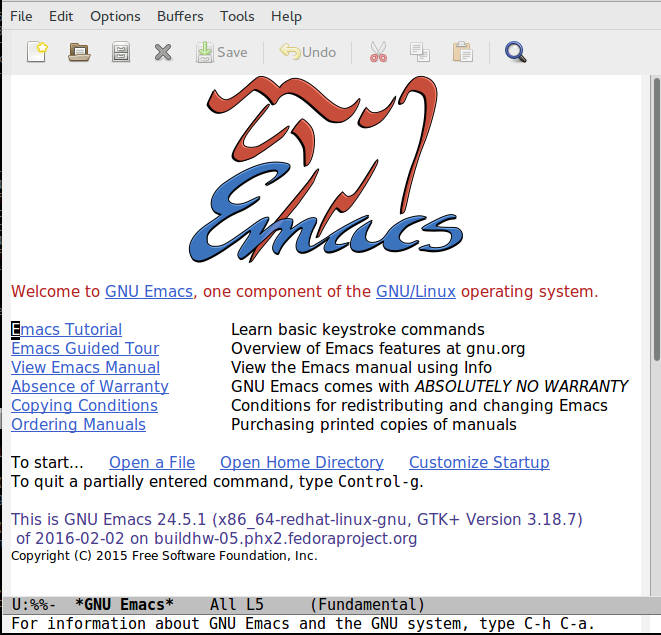
\includegraphics[width=8cm]{figures/emacs_welcome}
\caption{emacs Welcome Screen}
\label{emacsWelcomeScreen}
\end{figure}


So, at the Welcome Screen, you type \tbi{CTRL+h, release the keys and then type i}. You will get the next screen.

\begin{figure}[H]
\centering
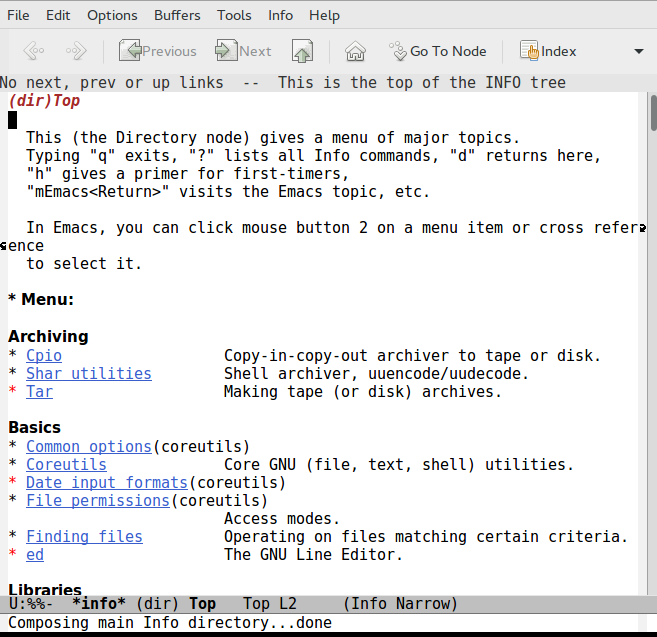
\includegraphics[width=8cm]{figures/emacs_listofinfocmds}
\caption{emacs info command list}
\label{emacsInfoCommandList}
\end{figure}

Now, we need to search for our command. We could just scroll down, but that is time consuming. Let's search for the \tbi{stat} command. Type: CTRL+s to start the search and then type: * (stat)

\begin{figure}[H]
\centering
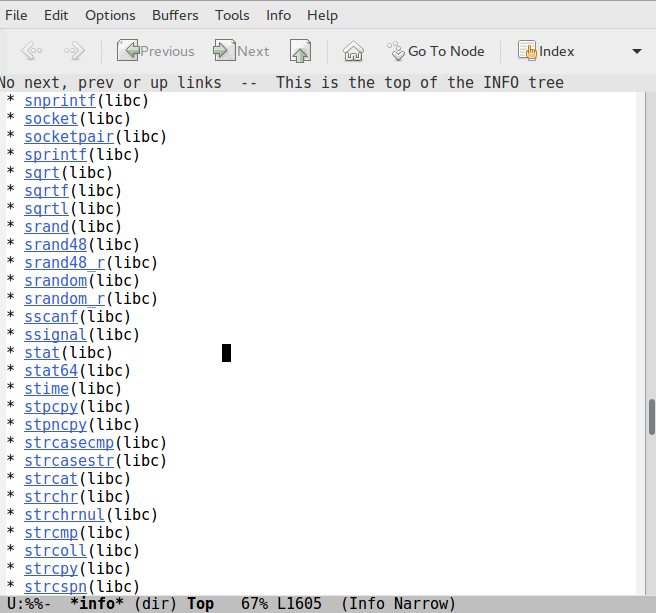
\includegraphics[width=8cm]{figures/emacs_statlist}
\caption{emacs stat entry in list}
\label{emacsStatList}
\end{figure}

Now, simply click on the \tbi{stat} link and the info page opens.

\begin{figure}[H]
\centering
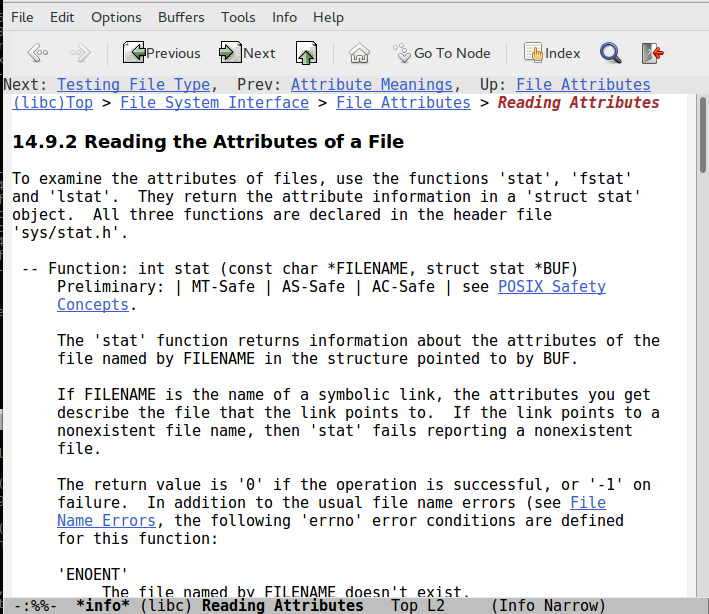
\includegraphics[width=8cm]{figures/emacs_statinfo}
\caption{emacs stat info document}
\label{emacsStatInfo}
\end{figure}

\subsection{coreutils}

Please visit \href{http://www.gnu.org/software/coreutils/coreutils.html}{Coreutils - GNU core utilities}. The following description is provided:

\begin{lstlisting}
The GNU Core Utilities are the basic file, shell and text manipulation utilities of the GNU operating system. These are the core utilities which are expected to exist on every operating system. 
\end{lstlisting}

Any command that is part of the GNU operating system will make reference to the \href{https://www.gnu.org/software/coreutils/manual/coreutils.html#Top}{GNU Coreutils} website. You will find very detailed information on each command.

\begin{lstlisting}[escapeinside={¿}{¿},frame=single,breaklines]
#
# Again, I use ¿\color[rgb]{0.133,0.545,0.133}\latex¿ to add the live hyperlink.
#
¿\tld¿ man ls | grep -A5 "SEE ALSO"
SEE ALSO
Full documentation at: <¿\href{http://www.gnu.org/software/coreutils/ls}{http://www.gnu.org/software/coreutils/ls}¿>
or available locally via: info '(coreutils) ls invocation'
\end{lstlisting}

\subsection{Developers Home Page}

Open source developers typically provide a man page. In one of the previous sections we installed the \keyword{lv} package . Note, the man page provides a link to the developer website.

\begin{lstlisting}[escapeinside={¿}{¿},frame=single,breaklines]
#
# Wouldn't it be nice if manpages had live hyperlinks?  ¿\color[rgb]{0.133,0.545,0.133}\emph{Brush up on your Japanese before clicking this link.}¿
#
¿\tld¿ man lv | grep -A5 "SEE ALSO"
SEE ALSO
LV Homepage: ¿\href{http://www.ff.iij4u.or.jp/\textasciicircum{}nrt/lv/}{http://www.ff.iij4u.or.jp/\ttbb{}nrt/lv/}¿

COPYRIGHT
All rights reserved. Copyright (C) 1996-2004 by NARITA Tomio.
\end{lstlisting}

\subsection{Searching all local resources for best information}

So, we have a number of ways of getting information on a particular command. Let's explore using \keyword{sed}. Note, we are only looking for a reference to the -e option. We may have to open the full man page or the full info document if the information is too cryptic to be helpful and then search inside the full document.

\begin{lstlisting}[escapeinside={¿}{¿},frame=single,breaklines]
#
# Suppose we know that sed has a -e option, but we forgot what that option actually did.
#
# 1. We could use my m- function. I use grep's -w, word option for an exact match. My function is very concise. It just says, yes there is a -e option.
#
¿\tld¿ m- sed | grep -w \\-e
-e script, --expression=script
#
# What about the man page? Note, I added grep's 'after lines of context' option, -A2. Well, this is a bit more helpful.
#
¿\tld¿ man sed | grep -A2 -w \\-e 
	-e script, --expression=script

	add the script to the commands to be executed
--
	If no -e, --expression, -f, or --file option is given, then the first non-option argument is taken  as  the sed  script  to  interpret.  All remaining arguments are names of input files; if no input files are specified, then the standard input is read.
--
	The comment extends until the next newline (or the end of a -e script fragment).

 }  The closing bracket of a { } block.
#
# How about the builtin --help function? Ok, that info is fairly similar to the man page info.
#
¿\tld¿ sed --help | grep -A3 -w \\-e
  -e script, --expression=script
				add the script to the commands to be executed
  -f script-file, --file=script-file
				add the contents of script-file to the commands to be executed
--
If no -e, --expression, -f, or --file option is given, then the first
non-option argument is taken as the sed script to interpret.  All
remaining arguments are names of input files; if no input files are
specified, then the standard input is read.
#
# Alright, let's try the info document? There is a ton of information. I only show a part of the output. As you can see, info really is the full documentation. I only show a small portion of the output. And, yes those backticks are correct...documentation that needs editing by the maintainer!
#
¿\tld¿ info sed | grep -C5 -w \\-e

If you do not specify INPUTFILE, or if INPUTFILE is `-', `sed'
filters the contents of the standard input.  The SCRIPT is actually the
first non-option parameter, which `sed' specially considers a script
and not an input file if (and only if) none of the other OPTIONS
specifies a script to be executed, that is if neither of the `-e' and
`-f' options is specified.

`sed' may be invoked with the following command-line options:

`--version'
--
By default, `sed' prints out the pattern space at the end of each
cycle through the script (*note How `sed' works: Execution Cycle.).
These options disable this automatic printing, and `sed' only
produces output when explicitly told to via the `p' command.

`-e SCRIPT'
`--expression=SCRIPT'
Add the commands in SCRIPT to the set of commands to be run while
processing the input.
.
.
\end{lstlisting}

So, what method should you use? It really depends on what you are looking for. I would suggest that you start with the simplest method and go to the more complex. 

\begin{enumerate}
	\item{my m- function}
	\item{-{}-{}help bash builtin command}
	\item{man page}
	\item{info document}
	\item{external resources on the web}	
\end{enumerate}

\section{Viewing man pages as html}

\subsection{TkMan}

\tbi{TkMan} is an open source package available at \href{https://sourceforge.net/projects/tkman/}{sourceforge}. Here is its description...

\begin{lstlisting}
TkMan is a graphical, hypertext manual page and Texinfo browser for UNIX.
TkMan boasts hypertext links, high quality display and a superior navigational interface,
full text search and much more.
\end{lstlisting}

\subsection{Searching online for manpages}

\begin{enumerate}
	\item{\href{http://grisha.biz/cgi-bin/man}{CentOS Man Pages}}
	\item{\href{http://linuxmanpages.net/index.html}{fedora manuals}}
\end{enumerate}

\subsection{Create a BROWSER environment variable}

\begin{lstlisting}[escapeinside={¿}{¿},frame=single,breaklines]
#
# You can also add this export statement to your .bashrc file.
#
¿\tld¿ export BROWSER=firefox
#
# Add the --html option and Firefox opens the ps manpage as an html document.
#
¿\tld¿ man --html ps
#
# This export statement can be added to your .bashrc file so that it is always available.
#
# We can also create an alias for this command: mh = man --html $1. We would then call it with: mh sed.
#
\end{lstlisting}

\section{Printing a man page}

\subsection{Creating a PDF}

\begin{lstlisting}[escapeinside={¿}{¿},frame=single,breaklines]
#
# First, using the man command itself, create a .ps, post script document.
#
¿\tld¿ man -t stat > stat.ps
#
# If you want to view the actual contents of stat.ps , issue the following command...
#
¿\tld¿ psnup stat.ps
%!PS-Adobe-3.0
%%Creator: groff version 1.22.3
%%CreationDate: Tue Mar 22 15:10:56 2016
%%DocumentNeededResources: font Times-Roman
.
.
%%Trailer
end
%%EOF
Wrote 2 pages, 14536 bytes
\end{lstlisting}

Now that you have a Post Script version of the manpage, open the file with a PDF reader such as the \href{https://help.gnome.org/users/evince/stable/}{Evince Document Viewer}.

\begin{figure}[H]
\centering
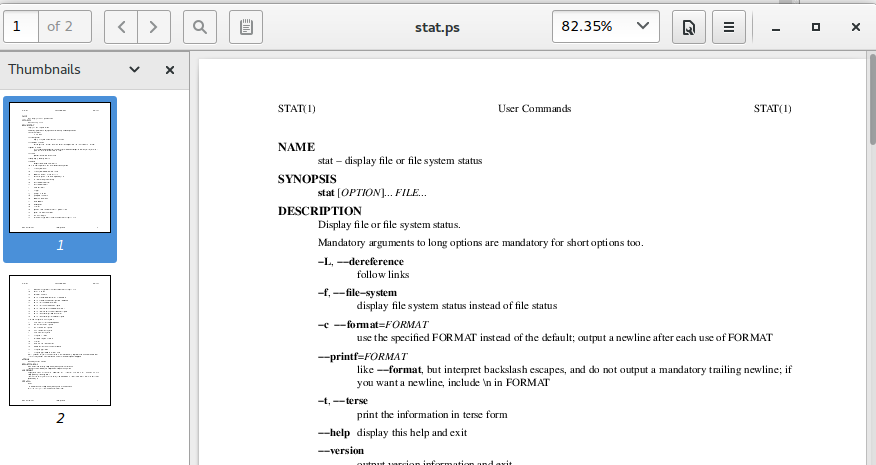
\includegraphics[width=12cm]{figures/statps}
\caption{stat Post Script}
\label{statPS}
\end{figure}

Now, all we have to do is CTRL+p to bring up the print controls. I assume that you have a local or network printer installed. This method allows you to view the man page as a PDF.\\

\subsection{Printing from the command line}

This is the easiet way to print a properly formatted man page.

\begin{lstlisting}[escapeinside={¿}{¿},frame=single,breaklines]
#
# Immediately print the texinfo manpage from the command line.
#
¿\tld¿ man -t texinfo | lpr -pPrinter
#
# Do you like this command? Add it to .bashrc. I will display the function that I added to .bashrc using the type command.  Add all the lines except the first to .bashrc. The type command adds the optional ; character. I did not  enter these when inputing the lines into .bashrc. So, type tells us 'best practices' for writing bash code.
#
¿\tld¿ type pman
pman is a function
pman () 
{ 
while [ $¿\#¿ -ne 0 ]; do
man -t $1 | lpr -pPrinter;
shift;
done
}
#
# Here is how these lines appear in my .bashrc file.
#
¿\tld¿ grep pman -A7 .bashrc
function pman ()
{
while [ $¿\#¿ -ne 0 ]
do
man -t $1 | lpr -pPrinter
shift
done
}
#
# Since the function reads all arguments supplied, we can print several man pages at once. The following command will print the texinfo and printf manpages.
#
¿\tld¿ pman texinfo printf
\end{lstlisting}

\chapter{Profiles}
\pagestyle{fancy}
\label{ch:profiles}

\fancyhf{} % here we clear any fancy header settings
%% Note, the first page of every chapter does not have a header.

\fancyhead[EC]{Linux System Administration} % E = even pages, C = center, rightmark defaults to number of current section
\fancyhead[OC]{\leftmark} % O=odd pages, C= center, leftmark defaults to Chapter number and title

%%
%% Set, headheight to eliminate warning message "Package Fancyhdr Warning: \headheight is too small (12.0pt): Make it at least 13.59999pt.
\setlength{\headheight}{13.6pt} 
%%
% The next line would put a line at the bottom of every page starting from the second page of every chapter, if it was uncommented.
%%
%\renewcommand{\footrulewidth}{1pt}
%%
\cfoot{\thepage} % c = center, foot = footer, thepage = page number
\rhead{
\includegraphics[width=.5cm]{figures/smCanadianFlag}}		
%%%%%%%%%%%%%%%%%%%%%%%%%%%%%%%%%%%%%%%%%%%%%%%%%%%%%%%%%%%
%%%%%%%%%%%%%%%%%%%%%%%%%%%%%%%%%%%%%%%%%%%%%%%%%%%%%%%%%%%

\section{Bash startup files}

Bash startup files or login scripts are the files that are read by the system at login. \emph{man bash} refers to these startup files and provides descriptions of their roles. Basically, there are two ways to start the shell: \emph{interactive login} and \emph{interactive non-login}. \emph{Interactive} means you can start entering commands and \emph{login} means that you got the shell after authenticating. After you are already logged on, you start an \emph{interactive non-login} session by opening a new shell or terminal window. You do this by simply typing the name of your shell, i.e., \emph{bash}. There are several startup files that the system attempts to load and read when logging on or starting a shell. Error messages are printed if these files are unreadable because of syntax errors. The system always reads the system startup file, but stops reading after a successful read of the first \emph{user} startup file encountered in the user's home directory.\\

Files read:

\begin{itemize}
	\item /etc/profile	- the system startup file
	\item \ttb{}.bash\_profile, \ttb{}.bash\_login, \ttb{}.profile, \ttb{}.bashrc - user startup files
	\item \ttb{}.bash\_logout - user logout file
\end{itemize}

\textcolor{red}{Linux Trivia:} bash = \href{https://en.wikipedia.org/wiki/Bourne_shell}{Bourne} Again SHell, rc=run control.

Note: As per \textsl{/etc/profile} all system-wide \hyperref[subsec:functions]{functions} and \hyperref[subsec:aliases]{aliases} should go in \textsl{/etc/bashrc}. You should not edit this file, nor should you edit any system file when you have the option to use alternative files. Instead, create custom shell files such as \textsl{custom.sh} and place them in \textsl{/etc/profile.d}. This folder was created by the kernel for this specific purpose.
%%%%%%%%%%%%%%%%%%%%%%%%%%%%%%%%%%%%%%%%%%%%%%%%%%%%%%%%%%%

\subsection{Invoked as an interactive login shell: the  \ttb{}.bash\_profile file}

You typically login (authenticate) to your system while sitting at the machine. You can also remotely connect over a local network or over the Internet using a remote connection protocol such as \emph{ssh}. The \keyword{\ttb{}.bash\_profile} file is executed in order to configure your shell prior to opening your command prompt window. To simplify things, \keyword{\ttb{}.bash\_profile} typically has lines of code that says go look for \keyword{\ttb{}.bashrc}; and if you find it, execute it. Therefore, I modify just \keyword{\ttb{}.bashrc} since my \keyword{\ttb{}.bash\_profile} file calls \keyword{\ttb{}.bashrc} with these lines of code...


\begin{lstlisting}[escapeinside={¿}{¿},frame=single,breaklines]
#
# Does the file '.bashrc' exist in your home directory?
# If yes, run it, otherwise, do nothing, end test.
#
if [ -f ¿\ttb¿.bashrc ]; then	
. ¿\ttb¿.bashrc
fi
\end{lstlisting}


\subsection{Invoked as an interactive non-login shell: the  \ttb{}.bashrc file}

When you are already logged on, you can open a new terminal window by typing the name of your shell: \tbi{bash}, \tbi{sh}, \tbi{tsh}, etc. Prior to opening the new terminal window, your \ttb{}.bashrc file is executed again when your shell is \tbi{bash}. 

%%%%%%%%%%%%%%%%%%%%%%%%%%%%%%%%%%%%%%%%%%%%%%%%%%%%%%%%%%%
%%%%%%%%%%%%%%%%%%%%%%%%%%%%%%%%%%%%%%%%%%%%%%%%%%%%%%%%%%%

\section{\ttb{}.bashrc}

\subsection{Making changes to \ttb{}.bashrc}
\label{subsec:makingchangesto-bashrc}

When you edit \ttb{}.bashrc you must re-load it in order for the changes to come into effect. You can logoff, which is very inefficient; or you can issue one of these commands:

\begin{lstlisting}[escapeinside={¿}{¿},frame=single,breaklines]
¿\tld¿ source .bashrc	# If you are in your home directory.
¿\tld¿ source ¿\ttb¿ .bashrc	# If you are not in your home directory.
¿\tld¿ . .bashrc	# That's a period followed by a space followed by .bashrc
¿\tld¿ . ¿\ttb¿ .bashrc	# If you are not in your home directory.
¿\tld¿ /bin/bash	# This opens a subshell in your terminal window and re-reads .bashrc. Type exit to close the subshell and return to the root window.
\end{lstlisting}

NOTE: \keyword{\ttb{}.bashrc} is read per shell window. \hyperref[subsec:terminator]{Terminator} is an app that let's you create a grid of terminal windows. You must refresh \ttb{}.bashrc in each terminal window after you make a change to \ttb{}.bashrc...if you want the change to be active in each window. Even if you just use the OS's builtin terminal program and have several individual windows open, you would have to refresh \ttb{}.bashrc in each window.

However, there is an alternative. You can add the following lines of code to \ttb{}.bashrc. After you do this, you must reload \ttb{}.bashrc in every terminal window for the change to take effect in the currently opened windows.  But, from this point onwards all you need to do is hit the enter key.

Basically, the code takes a time stamp of \ttb{}.bashrc when a new terminal is opened or when you hit enter and stores this time stamp in a variable. Every time you hit enter while in a terminal, the script compares the current time with the current time stamp on \ttb{}.bashrc. If the time stamp comparison is not equal, \ttb{}.bashrc is refreshed/reloaded.

\begin{lstlisting}[escapeinside={¿}{¿},frame=single,breaklines]
bashrc_sourced=$(stat -c %Y ¿\ttb¿.bashrc)
PROMPT_COMMAND='
test $(stat -c %Y ¿\ttb¿.bashrc) -ne $bashrc_sourced && source ¿\ttb¿.bashrc'
\end{lstlisting}

\subsection{Defining custom colours in \ttb{}.bashrc}\label{sec:customcolours}

I apologize to the person who wrote these codes lines, but I do not remember where I found them. It may have been from \href{https://help.ubuntu.com/community/CustomizingBashPrompt}{Customizing Bash Prompt.} You can define your own custom colours and then refer to them in your scripts...and in your \textsl{.bashrc} file. You will see in the \emph{Functions} section of my \textsl{.bashrc} file that I use the custom colour definitions when defining my command prompt functions. The following lines of code are in my \textsl{.bashrc} file. One's command prompt is customizable and \keyword{PS1} is an environment variable that defines the format of your command prompt.

\begin{lstlisting}[escapeinside={¿}{¿},frame=single,breaklines]
# ANSI color codes
RS="\[\033[0m\]"    # reset
HC="\[\033[1m\]"    # hicolor
UL="\[\033[4m\]"    # underline
INV="\[\033[7m\]"   # inverse background and foreground
FBLK="\[\033[30m\]" # foreground black
FRED="\[\033[31m\]" # foreground red
FGRN="\[\033[32m\]" # foreground green
FYEL="\[\033[33m\]" # foreground yellow
FBLE="\[\033[34m\]" # foreground blue
FMAG="\[\033[35m\]" # foreground magenta
FCYN="\[\033[36m\]" # foreground cyan
FWHT="\[\033[37m\]" # foreground white
BBLK="\[\033[40m\]" # background black
BRED="\[\033[41m\]" # background red
BGRN="\[\033[42m\]" # background green
BYEL="\[\033[43m\]" # background yellow
BBLE="\[\033[44m\]" # background blue
BMAG="\[\033[45m\]" # background magenta
BCYN="\[\033[46m\]" # background cyan
BWHT="\[\033[47m\]" # background white

force_color_prompt=yes
#
# Please also read the next section: ¿\hyperref[subsec:funkyprompts]{Functions and changing command prompts.}¿ 
#
# Simplest with color red.
#
PS1="{\h}$FRED[\W]$ $RS"
#
# Here is how the command prompt would appear...
#
¿\{LIB2015\}\color{red}\tld¿ 
#
# Here is another command prompt with time in color blue.
#
PS1="\[\033[1;34m\][\$(date +%H%M)][\w]#\[\033[0m\] "
#
#
# Here is how this command prompt would appear...the time is 12:51 p.m.
#
¿\color{blue}[1251]\tld\#¿ 
#
# Yet another command prompt! Two command lines are needed to define this command prompt. We first define a variable called: TTYNAME. We then use this variable in our second command which actual defines the prompt.
# 
# Set variable: TTYNAME=`tty|cut -b 6-`
#
TTYNAME=`tty|cut -b 6-`
# 
# Define the actual command prompt.
#
PS1="\[\033[32m\]\u@\h\[\033[33m\]($TTYNAME)\n\[\033[31m\][\w]#\[\033[0m\] "
#
# Two lines: 
# First is user@host{green} (pts{blue})
# Second line is [full path to current directory]#{red}
#
# And here is how our prompt appear. Note, the command prompt has two lines. 
#
¿\color{green}{mgcr@LIB2015}\color{blue}{(pts/1)}¿
¿\color{red}{[\ttb{}scripts]\#}¿
#
# u=user, h=host, n=newline, w=full path to current working directory. When [ and ] are preceded by a backslash, they are interpreted literally for the second line. The rest of the values inside the square brackets are for colors.
#
# We could also define our prompt in a single line using commnad substitution.
#
PS1="\[\033[32m\]\u@\h\[\033[33m\](`tty | cut -b 6-`)\n\[\033[31m\][\w]#\[\033[0m\] "
#
# So, I hope this example illustrates the potential for designing a custom command prompt.
#
\end{lstlisting} 


\section{Aliases}\label{sec:aliases}

A Bash alias is essentially a keyboard shortcut, an abbreviation, a means of avoiding typing a long command sequence. Pay particular attention to the different types of quotation marks. They can be quite tricky and may generate errors if you use them in the wrong context.

Alias definitions can go in \ttb{}.bashrc or alternatively you can create a \ttb{}.bash\_aliases file and place your aliases in that file. If you do this, include the following lines in your \ttb{}.bashrc file. This code says: check to see if there is a file called \ttb{}.bash\_aliases, if so, then read that file.

\begin{lstlisting}[escapeinside={¿}{¿},frame=single,breaklines]
#
# Note, there is a space after [ and before ]. As well, in the second line there is a space after the initial period.
#
if [ -f ¿\ttb¿.bash_aliases ]; then
. ¿\ttb¿.bash_aliases
fi
\end{lstlisting}

\subsubsection{user specific aliases}

\begin{lstlisting}[escapeinside={¿}{¿},frame=single,breaklines]
#
# I have many aliases in my ¿\ttb¿.bashrc file, how do I get a list of these aliases? Just grep all lines in ¿\ttb¿.bashrc containing the string" alias. Note: I will get an uncommented list of all aliases. I have added the comments to explain each alias.
#
¿\tld¿ grep alias .bashrc
#
# My user-specific aliases follow...
#
# Prompt for confirmation before removing files.
#
alias rm='rm -i'
#
# Prompt before overwrite when copying a file.
#
alias cp='cp -i'
#
# Prompt before overwrite when moving a file.
#
alias mv='mv -i'
#
# The mount command by itself presents information that is jumbled together and hard to read. By piping to 'column -t', the information is displayed in a tabular format.
#
alias mt='mount | column -t'
#	
# Clear the screen.
#
alias c='clear'
#	
# Get the setting for a specific environment variable. For example, the output of the command, pe hostname, will be: HOSTNAME=LIB2015. Without the pipe to grep, the output is simply: LIB2015. The tr command converts lower case to upper case. Environment variables are always in upper case.
#
alias pe='echo $1 | tr '[a-z]' '[A-Z]' | xargs printenv | grep -i $1' 
#
# Like mount, the fstab output is hard to read. This next alias places the output of fstab in columnar output.
#
alias ft='cat /etc/fstab | grep -v "^#" | column -t' 
#
# r for repeat, just repeat the last command in command history.
#
alias r='fc -s'	
#
# The switches for the manpage of cpio are preceeded by either [ or `. Therefore,  my m- function will not work with cpio.
#
alias mc-='man cpio | col -b | grep "^\ *.-"' 
#
# Go up one directory level.
#
alias ..='cd ..'
#
# Go up two directory levels.
#
alias ...='cd ../..'
#
# Go up three levels.
#
alias ....='cd ../../..'
#'
# I just want the lines with arguments in bash's builtin manpage.
#
alias mbi='man builtin | col -b | grep "^\ *.*\ *\["'
#	
# Get a long-listing of files with classification symbol at end: /=directory, nothing=normal file, *=executable, @=linked file.
#
alias lF='ls -alF'
#
# Gracefully reboot the computer, there are two ways.
#
alias srn='sudo shutdown -r now'
alias rbt='sudo reboot'
#
# Gracefully shutdown the computer.
#
alias shn='sudo shutdown -h now'
#
# Simplify the history and 'jobs -l' commands.
#
alias hy='history'
alias j='jobs -l'
#
# Temporarily unalias an alias.  Example, to unalias the alias, j = jobs -l, type: u j. In order to re-alias just: source \ttb{}.bashrc.
# 
# ¿\textbf{\color{red}Challenge:} If you use the time stamp code listed in \hyperref[subsec:makingchangesto-bashrc]{Section 5.2.1}, what happens after you unalias an alias and hit enter? \hyperlink{oj}{Answer}¿ 
#
alias u='unalias $1'
#
# Do you want to learn bash? Read the manpages for builtin and bash!
#
alias mbn='man builtin'
alias mb='man bash'
#
# Fedora used to use the yum package manager, but then switched to dnf.  I previously had the alias: alias yu='sudo yum update'. I can not use a similar alias called du since du is a builtin command. Therefore, I continue to use yu as the alias to update my system, the underlying definition just reflects the new package manager.
#
alias yu='sudo dnf update'.
#
# Install a package without interactively confirming the install...you are absolutely sure you want to install the package! I rarely use this alias since I like to see what dependency packages get installed when I install a package.
#
alias yy='sudo dnf -y $1'

# List only hidden files.
alias lf.='ls -A -1 -d -F .* | grep -v '/$''

# List only hidden directories.
alias ld.='ls -la -d .* | grep '^d''

# List hidden files and hidden directories.
alias lfd.='ls -la -d .* --color=auto'

# List hidden files and hidden directories with directories listed first.
alias lfd..=' ls -la -d .*  --group-directories-first'

# List both hidden and non-hidden directories.
alias ld='ls -la | grep '^d''

# List both hidden and non-hidden files.
alias lf='ls -la | grep -v '^d''
#
# I have two versions of Eclipse, a programming IDE, on my system. This alias just points to my special version.
#
alias eclipsee='/usr/bin/eclipsee'
#
# Note, in our alias list above, we had aliases for changing directory level by one, two, and three previous levels using two, three, and four periods respectfully. What would happen if we just typed one period?
#
¿\tld¿ .
bash: .: filename argument required
.: usage: . filename [arguments]
#
# Recall from the Programming chapter that the single period is a special character and is used to call a script or program from the current directory.
#
\end{lstlisting}

\subsubsection{system and user specific aliases from \ttb{}.bashrc}

A interesting challenge is how to get \emph{system aliases}. If you type just \textsl{alias} at the command line you get a list of the aliases for a currently logged on user and the system aliases. Here is an indirect method of getting just system aliases. Create a user \emph{myuser} who has no aliases in her \ttb{}.bashrc file. Then, issue the command in the next code block.

\begin{lstlisting}[escapeinside={¿}{¿},frame=single,breaklines]
#
# You will be prompted for root's password.
#
¿\tld¿ su - myuser -c 'getent passwd myuser | cut -d: -f7' -c 'alias -p'
Password: 
alias egrep='egrep --color=auto'
alias fgrep='fgrep --color=auto'
alias grep='grep --color=auto'
alias vi='vim'
alias xzegrep='xzegrep --color=auto'
alias xzfgrep='xzfgrep --color=auto'
alias xzgrep='xzgrep --color=auto'
alias yu='sudo dnf update'
alias zegrep='zegrep --color=auto'
alias zfgrep='zfgrep --color=auto'
alias zgrep='zgrep --color=auto'
\end{lstlisting}

Explanation: 

\begin{itemize}
	\item \textbf{su - myuser} - run the command as user \emph{myuser}. 
	\item \textbf{-c \tqs{getent passwd myuser | cut -d: -f7}} - run this command (-c): \tqs{getend passwd myuser} says list the password information for \emph{myuser} but only get the seventh field which happens to be the user's shell such as \textsl{/bin/bash}.
	\item \textbf{-c \tqs{alias -p:}} - run this command (-c) - print a list of all aliases
\end{itemize}

For any logged on user, we can also just issue the \keyword{alias} command and we will get aliases defined in our \ttb{}.bashrc file...as well as system aliases. The system aliases are defined in files located in the \textsl{/etc/profile.d} directory. In this directory, there are both \textsl{.csh} and \textsl{.sh} files. The former are for the \keyword{c-shell} and the later for the \keyword{bash-shell}. Examples are: \textsl{/etc/profile.d/colorls.sh} and \textsl{/etc/profile.d/colorgrep.sh}. So to conclude, we can get the aliases for any user account:

\begin{lstlisting}[escapeinside={¿}{¿},frame=single,breaklines]
¿\tld¿ su - useracct -c 'getent passwd useracct | cut -d: -f7' -c 'alias -p'
\end{lstlisting}

What is also interesting is that the above \emph{su -} command also works for \tbi{domain users}. If we issue the command \emph{cat /etc/passwd}, we get a list of all local accounts. Domain user accounts are not listed in this file. There are many ways to join a \tbi{domain}. This topic of domains is beyond the scope of this paper. However, the path to the home directory for domain users will typically be: \textsl{/home/domain.com/username}. To use the \emph{su -} command above, you only need the \emph{username}. You do not have to specify the domain.

\subsection{aliases for non-system users}

I found this script on the web script which lists the \href{http://unix.stackexchange.com/questions/237398/how-to-list-all-the-alias-for-all-the-user-have-on-my-linux-box-from-root}{aliases for all non-system users}. You must run this code as \keyword{sudo} or you will be prompted for each user's password. Also, it only lists aliases for local accounts, not domain accounts. I show the output for only two accounts: nfsnobody (there are no aliases) and for mgc.

\begin{lstlisting}[escapeinside={¿}{¿},frame=single,breaklines]
¿\tld¿ cat useraliases.sh 
¿\tbi{\#}¿! /bin/bash

for user in $(getent passwd | cut -d: -f1) ; do
	uid=$(getent passwd "$user" | cut -d: -f3)
	if [ "$uid" -ge 1000 ] ; then
		ushell=$(getent passwd "$user" | cut -d: -f7)
		[ -z "$ushell" ] && ushell='/bin/sh'
		echo "aliases for $user:"
		if [[ "$ushell" =~ /s?bin/(true|false|sync|ftponly|nologin) ]] ; then
			:
		elif [[ "$ushell" =~ /s?bin/(t?csh|zsh|s?ash) ]] ; then
			su - "$user" $ushell -c 'alias'
		elif [[ "$ushell" =~ /s?bin/([bd]ash|m?ksh|sh) ]] ; then 
			su - "$user" $ushell -c 'alias -p'
		fi
		echo ; echo
	fi
done
#
# Sample output...
#
¿\tld¿ sudo ./useraliases.sh
aliases for nfsnobody:

aliases for mgc:
Password: 
alias egrep='egrep --color=auto'
alias fgrep='fgrep --color=auto'
alias grep='grep --color=auto'
alias vi='vim'
alias which='(alias; declare -f) | /usr/bin/which --tty-only --read-alias --read-functions --show-tilde --show-dot'
alias xzegrep='xzegrep --color=auto'
alias xzfgrep='xzfgrep --color=auto'
alias xzgrep='xzgrep --color=auto'
alias zegrep='zegrep --color=auto'
alias zfgrep='zfgrep --color=auto'
alias zgrep='zgrep --color=auto'
.
.
\end{lstlisting}
 
\subsection{Overriding alias definitions}
 
 We can easily override aliases. The \emph{rm=\tqs{rm -i}}  alias uses the interactive -i switch. With this alias, anytime that you issue the \keyword{rm} command, you will be prompted for confirmation that you do wish to delete each file. This is a safety mechanism. It is very easy to kill your system if you by mistake issue the \emph{rm *} command (remove all) in a system directory. But, if you are in your \textsl{Downloads} directory, you may want to avoid the confirmation process for each file. You can override the alias, by preceding the command with a backslash.  So, type \emph{{\textbackslash}rm} instead of \emph{rm}.
 
\section{Functions}\label{sec:functions}

I like simplicity and shortcuts that eliminate the amount of typing I have to do.  Functions are more powerful than simple \emph{alias} commands and they make it easier to invoke commands that have complex syntax and/or require multiple arguments. As well, we can use \emph{bash programming} to create our functions. Functions like aliases can be placed in our \textsl{.bashrc} file or you can create a separate file called \textsl{.bash\_functions} or \textsl{.functions} and call that file from \textsl{.bashrc}.

In the following code, you will encounter several functions related to \keyword{manpages}. I find endless scrolling through manpages hunting for specific information to be very unproductive. I wanted an easy way to get snippets of information. Will you find these functions useful? \textit{Even if you don't use them, study them.} You may learn some \keyword{bash programming}!

\begin{lstlisting}[escapeinside={¿}{¿}, breaklines]{bash}

function h()
#
# Type 'h cmd' instead of 'cmd --help'
#
{
echo "--help" | xargs $1
}

function tu ()
#
# tr is the translate command, here we are converting lower-case to upper-case, $1 is the string to convert. Example: tu bob, returns BOB
{
echo $1 | tr '[a-z]' '[A-Z]'
}

function tl ()
#
# tr is the translate command, here we are converting upper-case to lower-case, $1 = string to change. Example: tl BOB , returns bob.
#
{
echo $1 | tr '[A-Z]' '[a-z]'
}

function manh ()
#
# Section headers in manpages are in upper case. 
# This function can be used to display the manpage between two section headers.
# Task: Display only the section of the sed manpage for between 'DESCRIIPTION' and 'COMMAND SYNOPSIS', that is, only the 'DESCRIPTION' section of the sed manpage.
# Example: manh sed description "command synopsis"
# As above, if the section header has spaces, place the section header in double parenthesis.
# We use the tr command to change section headers to uppercase, so we do not have to type the section header in upper case.
# $1 = command $2 = first header and $3 = second header
# sed switches: n=silent, p=print
# Pipe to less in case the section is quite long.
# Note: if you get a blank window, you mispelled a header.
# Piping to, sed '$d', removes the last line which is the second section header.
# Pay attention! I am using grave accents, command substitution, to define the variables b and e.
#
{
b=`echo $2 | tr '[a-z]' '[A-Z]'`
e=`echo $3 | tr '[a-z]' '[A-Z]'`
man $1 | col -b| sed -n "/$b/,/$e/p" | less | sed '$d'
}

function mana()
# Here we use 'grep -ix' instead of tr to tell the command to ignore case.
# Task: Print out a number of lines after the beginning of a manpage section.
# Example: print out 5 lines of the synopsis header section of the sed manpage.
# $1 = command, $2 = section header, $3 = number of lines
# Note: The command did not work unless I first assigned $3 to a variable name. I could not use $3 directly in the command.
#  Example: mana sed synopsis 5
#
{
n=$3
man $1 | col -b | grep -ix $2 -A$n
}

function mans ()
#
# Get a list of all section headers of a man file, e.g., mans sed.
#
{
man $1 | grep '^[A-Z]'
}

function m- ()
#
# Get a list of all the command switches in the manpage, those lines beginning with a minus sign. The output is similar to: 'cmd --help' whose output is quite verbose. The output of 'm- cmd' is quite concise. For example, instead of typing 'sed --help', you can type 'm- sed'.
# 
# grep's regex explained: ^ means at beginning of line. \ escapes the next character (take this character literally, the space).  * means any number of the preceding character, the space. Then, an actual minus sign. Then, any character, represented by the period.
#
# $1 = the command, col -b is used to format the man page. Try the command without the formatting section, | col -b |, especially when sending the output to a file.
#
Example: m- sed
#
{
man $1 | col -b | grep "^\ *-."
}

function m-- ()
#
# This function is related to my m- alias. Some man pages do not precede their options with spaces followed by a minus sign. Instead, the spaces are followed  but some other character. So, if the function m- does not work, use m--. Note the placement of the period.
#
{
man $1 | col -b | grep "^\ *.-"
}

function cm()
#
# See ¿\hyperref[sec:topcpu]{Finding top consumers of CPU resources}¿ for alternative.
# With the ps command, the third column of output is %CPU and the fourth is %MEM.
# This function takes two switches: sort column (3 or 4 )and number of lines.
#
# Example: top four processes sorted on %CPU in descending order.
# cm 3 4
#
# When you pipe the 'ps auxf' command, the headers are removed. 'ps auxf | head -1' just prints the header line.
#
{
p=$1
n=$2
echo "Top processes: "; ps auxf | head -1 && ps auxf | sort -nr -k $p | head -$n;
}

function mang()
#
# This is another way of printing a section of a manpage. The function changes section headers to uppercase using the echo and tr commands.
#
# Use the -A (# of lines after) and -B (# of lines before) grep switches with large values in order to  ensure we just capture the required section. Think about how the overlap works. Sketch it out.
#
# $1 = manpage $2 = first section header and $3 = second section header
# Remove the last pipe, | sed '$d', and see what happens.
# Example: mang sed name synopsis
# 
{
b=`echo $2 | tr '[a-z]' '[A-Z]'`
e=`echo $3 | tr '[a-z]' '[A-Z]'`
man $1 | col -b| grep -A1000 -x "$b" | grep -B1000 -x "$e" | sed '$d'
}

function mbib()
#
# There are a large number of topics within each manpage header in the 'builtin' manpage. If we know that the bind section is followed by the break section, we can issue the following command:
#
# mbib bind break
#
# $1 = 1st header and $2 = second header
# 
# With this function, I am using the grep block option which is equivalent to the grep -x, exact option.
#
{
man builtin | col -b | grep -A1000 "^\ *\b$1\b" | grep -B1000 "^\ *\b$2\b" | sed '$d'
}
#
# In the next three functions, I illustrate how to create custom command prompts. To invoke them, simply type their name.
#
function p3()
{
#
# See ¿\hyperref[sec:customcolours]{Section~ 5.2.5}¿, defining cutsom colours in .bashrc.  This command prompt is simply the cirumflex inside square brackets. FRED=foreground red, RS=reset, PS1=command prompt environment variable.
#
PS1="$FRED¿\tld¿ $RS"
}

function p2()
#
# Just type: p2
# A different command prompt with time of day: hh:mm.
#
{
PS1="\[\033[1;34m\][\$(date +%H:%M)][\w]$\[\033[0m\] "
}

function p1()
#
# Just type: p1
# This is similar to my default command prompt. The full path of the current working directory is shown followed by the dollar sign. The hostname is not shown. 
#
{
PS1="$FRED[\w]\$ $RS"
}

function p0()
#
# My default prompt.
#
{
PS1="{\h}$FRED[\W]$ $RS"
}

function cn()
#
# This is just a command to open a local .html file on my system. Just type cn and Firefox opens the local .html file. The & at the end of the command returns the command prompt so that it is available again. The process to launch Firefox process remains in the background, but Firefox runs in the foreground.
#
{
firefox /home/mgcr/coursera/uwhpsc/notes/_build/html/index.html &
}
\end{lstlisting}

\subsection{Functions and changing command prompts}\label{subsec:funkyprompts}

I will illustrate the different command prompts. I start with my default prompt and end with my default prompt. I call new prompts by issuing one of the prompt functions defined above. Note, the final character of my command prompt is the dollar sign except for the \emph{p3} command prompt. Note, I am also showing actual colours to represent the colours specified in the definition of each command prompt.

\begin{lstlisting}[escapeinside={¿}{¿}, breaklines]{bash}
#
# w=full path, W=last level (deepest) of full path, h=hostname. Remember: the tilde is a builtin shortcut for the home directory!
#
{LIB2015}¿\textbf{\color{red}[\ttbb{}]\$}¿ pwd
/home/mgcr

{LIB2015}¿\textbf{\color{red}[\ttbb{}]\$}¿ echo $PS1
{\h}\[\033[31m\][\W]$ \[\033[0m\]
#
# So, I am using my default command prompt. Let's switch to the p1 command prompt.
#
{LIB2015}¿\tld¿$ p1
¿\textbf{\color{red}[\ttbb{}]\$}¿ echo $PS1
\[\033[31m\][\w]$ \[\033[0m\]
#
# Ok, let's switch to the p2 command prompt.
#
¿\tld¿$ p2
¿\textbf{\color{blue}[18:45][\ttbb{}]\$}¿ echo $PS1
\[\033[34m\][$(date +%H:%M)][\w]$\[\033[0m\]
#
# Finally, let's switch to the p3 command prompt.
#
¿\textbf{\color{blue}[18:45][\ttbb{}]\$}¿ p3
¿\textbf{\color{red}[\ttbb{}]}¿ echo $PS1
\[\033[31m\]¿\tld¿ \[\033[0m\]
#
# Change to a different directory and cycle through the different command prompts.
#
¿\textbf{\color{red}[\ttbb{}]}¿ cd scripts
¿\textbf{\color{red}[\ttbb{}]}¿ p1
¿\textbf{\color{red}[\ttbb{}/scripts]\$}¿ p2
¿\textbf{\color{blue}[18:48][\ttbb{}/scripts]\$}¿ p3
¿\textbf{\color{red}[\ttbb{}]}¿
#
# Go back to our default command prompt by issuing the p0 function call. Alternative, issue this command: source ~/.bashrc
#
¿\textbf{\color{red}[\ttbb{}]\$}¿ p0
{LIB2015}¿\textbf{\color{red}[scripts]\$}¿ echo $PS1
{\h}\[\033[31m\][\W]$ \[\033[0m\]
\end{lstlisting}

\section{History}

 The Bash \keyword{history} command is used to edit and manipulate one's command history in order to simplify re-entering previously-used commands. History parameters or settings are defined in your \textsl{\ttb{}.bashrc} file. All commands that you issue are tracked and recorded in the \textsl{\ttb{}.bash\_history} file.
 
 By default, the bash shell writes its history at the end of each session, overwriting the existing \textsl{\ttb{}.bash\_history} file with an updated version. This means that if you are logged in with multiple bash sessions, only the last one to exit will have its history saved. We can work around this with the \emph{shopt -s histappend} command...which will append to, instead of overwriting, the \textsl{\ttb{}.bash\_history} file.
 
 In the following example, \keyword{ignoreboth} = ignorespace and ignoredupes. \keyword{ignorespace} is a quick way to enter a command that you do not want as part of your history. You type a space, then the command, and then the enter key. The space before the command tells the bash shell not to include the command in command history. \keyword{ignore dupes}, of course, says only store unique commands in history, no duplicates.
 
\begin{lstlisting}[escapeinside={¿}{¿},frame=single,breaklines]
#
# Set history file length (number of lines) with this command.
#
HISTFILESIZE=1000000 
#
# This is the number of lines loaded into memory, it can be equal to or less than the HISTFILESIZE metric.
#
HISTSIZE=1000000
#
# Don't put duplicates in history nor commands that begin with a space.
#
HISTCONTROL=ignoreboth
#
# Don't add these commands to history.
#
HISTIGNORE='ls:bg:fg:history:c:reboot:yu'
#
# The following updates history immediately on carraige return, not at end of bash session. A more useful setting is described in ¿\hyperref[subsec:makingchangesto-bashrc]{Section~ 5.2.1}¿?
#
PROMPT_COMMAND='history -a'
#
# Append to history file, don't overwrite.
#
shopt -s histappend 
\end{lstlisting}

\subsubsection{Calling specifc commands from history}

\begin{lstlisting}[escapeinside={¿}{¿},frame=single,breaklines]
¿\tld¿ history     # Numbered list of all commands stored in ¿\tldi{}¿/.bash_history.

¿\tld¿ history 662 # Execute history command number 662.

¿\tld¿ !662     # A more concise way to execute history command number 662 (no spaces between characters).

¿\tld¿ !-6     # Execute the 6th last command in history (no spaces between characters).

¿\tld¿ mkdir bob marley		# Make two directories bob and marley.

¿\tld¿ cd !^		# Change into directory bob, the first argument of the previous command.

¿\tld¿ mkdir bob marley		# Make two directories bob and marley.
#
# Change into directory marley, the last argument of the previous command. Instead of typing !$ you can also type: cd followed by a space and then alt. or esc. which will display marley.
#
¿\tld¿ cd !$	

¿\tld¿ mkdir bob marley		# Make two directories bob and marley.
#
# List the contents of bob and marley, that is, list all arguments of the previous command.
#
¿\tld¿ ls !*	
#
# When you are repeatedly testing a command, you may want to override the default behaviour of another command. For example, to test the above history argument shortcuts, I was creating the bob and marley folders and then deleting them in order to test the next command. I did not want to confirm my deletes, so I issued this command instead: '\rm -fr bob marley' instead of 'rm -fr bob marley'. The backslash says override the alias, 'rm -i', and use the system command instead, rm. With the alias version of rm, I would have had to confirm the deletion of the bob folder and the marley folder and each file inside of these folders.
#
¿\tld¿ touch file1 file2 file3 # Create three empty files.
#
# Echo the string "text" to the 2nd argument of the previous touch command, that is, send the string to and write to file2.
#
¿\tld¿ echo "text" > !touch:2 
¿\tld¿ cat file2 # Let's check, display the contents of file2.
text

¿\tld¿ locate mini.zip	# Where is the archive mini.zip?
/home/mgcr/Downloads/mini.zip
#
# Unzip this archive into the current directory, note $(!!) translates as the output of the last command so that the full command becomes: 'unzip /home/mgcr/Downloads/mini.zip'.
#
¿\tld¿ unzip $(!!)	
#
# Note, the locate command uses a database that gets updated on a daily basis (run by the kernel scheduler crond). If you create a new file and issue the command: locate newfile, nothing is returned. You have to first manually update the database by issuing this command: 'sudo /usr/bin/updatedb'. You will then be able to locate the newly created file. The above example assumes that the mini.zip file was created prior to the current day or that the database was manually updated.
#
# Execute the last'cat'command. After the command is executed, if you hit the up-arrow, the expanded command is displayed on the command line. The command is now available for editing or executing again.
#
¿\tld¿ !cat
#	
# Just print the last 'cat command'; up-arrow also displays the last 'cat' command on the command line ready to edit or execute.
#
¿\tld¿ !cat:p	

¿\tld¿ !!	# Execute the last command.

¿\tld¿ !!:p	# Just print-out the last command, up-arrow operates as above.
#
# !! is a very useful command. Suppose you issue a command that requires super user privilege. That is, you need to precede the command with sudo, but you forgot the sudo. Instead of hitting the up arrow and the home key and typing sudo in front of the command, just type: sudo !!, i.e., run the last command as super user. You have to be a sudo user in order to do this.
#
¿\tld¿ sudo !!	
#
# Read from history and list the last 10 commands issued (the default # is 10).
#
¿\tld¿ fc -l

¿\tld¿ fc -l -20      # Read from history and list the last 20 commands issued.
#
# grep (filter or show) only alias commands issued within the last 20 commands issued.
#
¿\tld¿ fc -l -20 | grep alias     

¿\tld¿ fc -s mystring     # Execute the last command beginning with string "mystring".

¿\tld¿ fc -l 671 681	# List commands from history numbers 671 to 681.
#
# List the most recent commands between last instance of ls and last instance of pwd.
#
¿\tld¿ fc -l ls pwd	
\end{lstlisting}

%%%%%%%%%%%%%%%%%%%%%%%%%%%%%%%%%%%%%%%%%%%%%%%%%%%%%%%%%%%
%%%%%%%%%%%%%%%%%%%%%%%%%%%%%%%%%%%%%%%%%%%%%%%%%%%%%%%%%%%

%%%%%%%%%%%%%%%%%%%%%%%%%%%%%%%%%%%%%%%%%%%%%%%%%%%%%%%%%%%
%%%%%%%%%%%%%%%%%%%%%%%%%%%%%%%%%%%%%%%%%%%%%%%%%%%%%%%%%%%
%%%%%%%%%%%%%%%%%%%%%%%%%%%%%%%%%%%%%%%%%%%%%%%%%%%%%%%%%%%
\chapter{Vi Text Editor}
\pagestyle{fancy}

\fancyhf{} % here we clear any fancy header settings
%% Note, the first page of every chapter does not have a header.
\fancyhead[EC]{Linux System Administration}
\fancyhead[OC]{\leftmark} % O=odd pages, C= center, leftmark defaults to Chapter number and title
%\fancyhead[EC]{\rightmark} % E = even pages, C = center, rightmark defaults to number of current section
%%
%% Set, headheight to eliminate warning message "Package Fancyhdr Warning: \headheight is too small (12.0pt): Make it at least 13.59999pt.
\setlength{\headheight}{13.6pt} 
%%
% The next line would put a line at the bottom of every page starting from the second page of every chapter, if it was uncommented.
%%
%\renewcommand{\footrulewidth}{1pt}
%%
\cfoot{\thepage} % c = center, foot = footer, thepage = page number
\rhead{
\includegraphics[width=.5cm]{figures/smCanadianFlag}}		
%%%%%%%%%%%%%%%%%%%%%%%%%%%%%%%%%%%%%%%%%%%%%%%%%%%%%%%%%%%
%%%%%%%%%%%%%%%%%%%%%%%%%%%%%%%%%%%%%%%%%%%%%%%%%%%%%%%%%%%

\section{Introduction}
How do Linux System Administrators interact with workstations and servers? The answer is that most LSA's work at the CLI, the \href{https://en.wikipedia.org/wiki/Command-line\_interface}{command line interface}. You sit physically in front of your system and type on a keyboard. Or, you remote into your system using a communication application or protocol. Typically, your typing is an editing process. You edit or create configuration files for applications or system daemons and you create documents. My favourite editing tool is \keyword{vi}.

\section{Overview of vi}
\tbi{vi} is a text editor that uses the keyboard to control everything...no mouse is needed. I have been using \emph{vi} since the days when Linux did not have a desktop, that is, no graphical environment. \emph{vi} is a wonderfully easy-to-use text editor, although one must memorize an odd assortment of commands and syntax.

Some readers may ask, "Easy-to-use, are you kidding me?" My response is that it is easy-to-use if you use only a small subset of \emph{vi's} feature set. However, you will work very inefficiently until you master the more complex commands and features.

Fortunately, \emph{vi} has a powerful online help tool that provides examples for each command. There are other popular text editors such as \href{https://www.gnu.org/software/emacs/}{emacs} and \href{http://www.nano-editor.org/}{nano}, but this chapter focuses only on \href{http://vim.wikia.com/wiki/Vim_Tips_Wiki}{vi/vim}.

\section{vi is vim}
In the early days of Linux, you typically could have both \tbi{vi} and \tbi{vim---Vi IMproved} installed on your system. \keyword{vim}, of course, has more features and capabilities. Today, you really only have \emph{vim} on your system, but the \emph{vi} command is still used to launch \emph{vim}. However, take note of the discussion that follows comparing \tbi{Vi IMproved} and \tbi{Vim-enhanced}.

\begin{lstlisting}[escapeinside={¿}{¿},frame=single,breaklines]
#
# I just want the first line of the vi versioning information.
#
¿\tld¿ vi --version | head -1
VIM - Vi IMproved 7.4 (2013 Aug 10, compiled Aug 20 2015 09:51:26)
\end{lstlisting}

If you just type \emph{vi} and hit the enter key at the command line, \emph{vi} will open and display the following splash-screen...which will disappear as soon as you start entering text.

\begin{center}
VIM - Vi IMproved\\
Version 7.4.827\\                                                 
by Bram Moolenaar et al.\\                                               
Modified by <bugzilla@redhat.com>\\                                       
Vim is open source and freely distributable\\                                     

Help poor children in Uganda!\\                                            
type  :help iccf<Enter>       for information\\                                     

type  :q<Enter>               to exit\\                                             
type  :help<Enter>  or  <F1>  for on-line help\\                                    
type  :help version7<Enter>   for version info \\    
\end{center}

The version of vi that comes with Fedora 23 is \emph{Vi IMproved}, not \emph{Vim-enhanced}. Why is this important? Well, you will soon find out that certain commands don't work with \emph{Vi IMproved}. Try splitting a \emph{vi} window vertically before you have \emph{Vim-enhanced} installed! When starting \emph{vi}, after you install \emph{Vim-enhanced}, it is interesting that you will get the same splash screen as shown. So, the splash screen does not tell you which version of \emph{vi} is installed.

I hope the exploration of this topic will help illustrate how I logically try to resolve technical issues. As I dig, as I explore, I discover new commands and I master new features of existing commands that I already know. I may start sounding rather pushy and pedantic, but \textit{don't just sit there and be confused, do some work, test some things, and don't be afraid to make mistakes...as long as you have several different types and sources of backups!} Why? At the worst possible moment, you may find that your only backup is corrupted or too outdated to be useful!

\subsection{vim-minimal}

We will see from the code below that the package \keyword{vim-minimal} is in fact \emph{Vi Improved}.

\why{Why does dnf provides show two repos for vi package, @system and fedora?}

\begin{lstlisting}[escapeinside={¿}{¿},frame=single,breaklines, language={bash},keywords={which,ls,type,dnf,rpm,sudo}]
#
# Which default vi package gets executed?
#
¿\tld¿ which vi
/bin/vi
#
# Does this path have a symbolic link? That is, does it actually point to another file? How do we determine whether it does or does not point to another file? One way is to issue the ls command with the all option. As we see, vi does not point to another file. 
#
¿\tld¿ ls -la /bin/vi
-rwxr-xr-x. 1 root root 1021960 Aug 20 02:52 /bin/vi
#
# If vi pointed to another file, we would see a symbolic link. So, what does a symoblic link look like? If we use the ls command, only the color will tell us whether or not the file has a symbolic link. I am going to use actual colors for the file lists to illustrate how symbolic links appear at the command line. The color of normal files will be white when your default is white foreground and black background. However, files with a symbolic link will be Aquamarine and executable files will be green in colour. I am using Latex's colors to show the distinction, so the colours will appear a bit off.
#
# The path /usr/sbin/telinit is Aquamarine in colour and this colour indicates that the file has a symbolic link, it points to another file.
#
¿\tld¿ ls /usr/sbin/telinit
¿\textbf{\color{Aquamarine}/usr/sbin/telinit}¿
#
# The path /usr/sbin/tc is green in colour which indicates that tc is an executable file.
#
¿\tld¿ ls /usr/sbin/tc
¿\textbf{\color{green}/usr/sbin/tc}¿
#
# The full file listing for tc is also in green and there is no indication of a symbolic link.
#
¿\tld¿ ls -la /usr/sbin/tc
-rwxr-xr-x. 1 root root 337072 Oct 26 13:26 ¿\textbf{\color{green}/usr/sbin/tc}¿
#
# However, we get both a color representation with a long listing for telinit and a clear indication that telinit has a symbolic link. Note, /usr/sbin/telinit points to /usr/bin/systemctl...which is in green and thus is an executable file.
#
¿\tld¿ ls -la /usr/sbin/telinit
lrwxrwxrwx. 1 root root 16 Feb  1 06:04 ¿\textbf{\color{Aquamarine}/usr/sbin/telinit}¿ -> ¿\textbf{\color{green}../bin/systemctl}¿
#
# A normal file will have the default foreground colour for both ls and ls -la. Latex's lstlisting package that I am using to display bash commands uses the colour blue to highlight bash commands.
#
¿\tld¿ ls myfile.txt
myfile.txt

¿\tld¿ ls -la myfile.txt
-rw-rw-r--. 1 mgcr mygrp 44869 Jan 20 10:24 myfile.txt

#
# We can also use the type command to verify that vi has no symbolic link.
#
¿\tld¿ type -a /bin/vi
/bin/vi is /bin/vi
#
# Ok, what package provided /bin/vi? We see below that it is vim-minimal.
#
¿\tld¿ dnf provides /bin/vi
Last metadata expiration check performed 21 days, 0:54:03 ago on Thu Dec 24 10:08:26 2015.
vim-minimal-2:7.4.827-1.fc23.x86_64 : A minimal version of the VIM editor
Repo        : @System

vim-minimal-2:7.4.827-1.fc23.x86_64 : A minimal version of the VIM editor
Repo        : fedora
#
# So, do we have vim-minimal? Let's check. The following command asks if vim-minimal is installed. As we can see it is installed.
#
¿\tld¿ dnf list installed vim-minimal
Last metadata expiration check performed 12 days, 20:00:28 ago on Tue Feb  2 13:41:23 2016.
Installed Packages
vim-minimal.x86_64                                   2:7.4.827-1.fc23                                   @@commandline
#
# We can also get this info using the rpm command. -q=query, -f=file
#
¿\tld¿ rpm -qf /bin/vi
vim-minimal-7.4.827-1.fc23.x86_64
#
# We use the following rpm command to  see what files vim-minimal installed. Old school!
#
¿\tld¿ rpm -ql vim-minimal
/etc/virc
/usr/bin/ex
/usr/bin/rvi
/usr/bin/rview
/usr/bin/vi
/usr/bin/view
/usr/share/man/man1/ex.1.gz
/usr/share/man/man1/rvi.1.gz
/usr/share/man/man1/rview.1.gz
/usr/share/man/man1/vi.1.gz
/usr/share/man/man1/view.1.gz
/usr/share/man/man1/vim.1.gz
/usr/share/man/man5/virc.5.gz
#
# The new school way...
#
¿\tld¿ dnf repoquery -l vim-minimal
/etc/virc
/usr/bin/ex
/usr/bin/rvi
/usr/bin/rview
/usr/bin/vi
/usr/bin/view
/usr/share/man/man1/ex.1.gz
/usr/share/man/man1/rvi.1.gz
/usr/share/man/man1/rview.1.gz
/usr/share/man/man1/vi.1.gz
/usr/share/man/man1/view.1.gz
/usr/share/man/man1/vim.1.gz
/usr/share/man/man5/virc.5.gz
#
# Does /usr/bin/vi point to /bin/vi?
#
¿\tld¿ type -a /usr/bin/vi
/usr/bin/vi is /usr/bin/vi
#
# At this point, I was at a loss as to why the command, dnf repoquery -l vim-minimal, did not show the /bin/vi path that the command, which vi, lists. Stay tuned! This will be partially explained in the next section of code. 
#
# However, we can confirm that vim-enhanced is not installed with this command. Note, I initially chose not to install the package (I answered n = no). In Linux, when you issue a command related to a package that is not installed, the kernel tries to suggest a package that may contain that command.
#
¿\tld¿ which vim
bash: vim: command not found...
Install package 'vim-enhanced' to provide command 'vim'? [N/y] n
#
# Alternatively, we could have said: dnf list installed vim-enhanced.
#
# So, let's go ahead and install vim-enhanced.
#
¿\tld¿ sudo dnf install vim-enhanced
¿\tld¿ which vim
/bin/vim
#
# Now, we could add an alias for vim in our ~/.bashrc. Why? We just want to type the vi command when starting vim. One fewer characters to type. Woopee! The alias would be: alias vi=vim
#
# Note, take a look at /etc/profile.d/vim.sh. Remember that any scripts in this directory are executed when we logon. So, we really do not need the alias in our .bashrc file.
#
¿\tld¿ cat /etc/profile.d/vim.sh | grep alias | grep -v grep
¿\tbi{\#}¿ for bash and zsh, only if no alias is already set
alias vi >/dev/null 2>&1 || alias vi=vim

\end{lstlisting}

\subsection{vim-enhanced}

Let's look at a couple of other commands in order to get a more complete picture of vi. We will see from the code below that the \keyword{vim} package is in fact \keyword{Vim-enhanced}.

\begin{lstlisting}[escapeinside={¿}{¿},frame=single,breaklines]
#
# Note, I did add that alias to my .bashrc file.
#
¿\tld¿ which vi
alias vi='vim'
/bin/vim
#
# So, we have an alias defined. This alias could have been defined in both our .bashrc file and/or in the system /etc/profile.d/vim.sh file. Let's override the alias by using the backslash in front of the which command to find the true path of vi.
#
¿\tld¿ \which vi
/bin/vi
#
# We found out from the previous section that the package that provided /bin/vi was vim-minimal.
#
¿\tld¿ rpm -qf /bin/vi
vim-minimal-7.4.827-1.fc23.x86_64
#
# Let's find out what package provides vim.
#
¿\tld¿ which vim
/bin/vim

¿\tld¿ dnf provides /bin/vim
Last metadata expiration check performed 21 days, 0:54:23 ago on Thu Dec 24 10:08:26 2015.
Error: No Matches found
#
# What happened here? The readlink command can be used to see if there is a realpath to another file. We can also once again override the which command.
#
¿\tld¿ readlink -e /bin/vim
/usr/bin/vim

¿\tld¿ \which vim
/usr/bin/vim
#
# Ok, let's use that path with 'dnf provides'. We see that the package vim-enhanced provides the vim executable.
#
¿\tld¿ dnf provides /usr/bin/vim
Last metadata expiration check performed 21 days, 1:10:54 ago on Thu Dec 24 10:08:26 2015.
vim-enhanced-2:7.4.827-1.fc23.x86_64 : A version of the VIM editor which includes recent enhancements
Repo        : @System

vim-enhanced-2:7.4.827-1.fc23.x86_64 : A version of the VIM editor which includes recent enhancements
Repo        : fedora
#
# Is there a similar realpath for /bin/vi?
#
¿\tld¿ readlink -e /bin/vi
/usr/bin/vi
#
# Hey, look at that.There is a reallink from /bin/vi to the executable /usr/bin/vi which is the file that the vim-minimal package actually installed. Mystery solved! You and I both need to readup on the readlink command.
#
# As shown in the previous section of code, we can also get path info using the type command.
#
# -a = all places that contain the executable
# -t = type, prints one of: alias, keyword, function, builtin, file
# -P = the path that gets executed when we type the name of the command
#
¿\tld¿ type -a vi
vi is aliased to 'vim'
vi is /bin/vi
vi is /usr/bin/vi
vi is /bin/vi
vi is /usr/bin/vi
vi is /usr/bin/vi

¿\tld¿ type -t vi
alias

¿\tld¿ type -P vi
/bin/vi
#
# Let's do the same for vim. Note: There is no vim alias.
#
¿\tld¿ type -a vim
vim is /bin/vim
vim is /usr/bin/vim
vim is /bin/vim
vim is /usr/bin/vim
vim is /usr/bin/vim

¿\tld¿ type -t vim
file

¿\tld¿ type -P vim
/bin/vim
#
# What about the command type itself? What type of file is it? We see that it is a builtin function. To just display the section of the builtin manpage that covers type, issue my .bashrc function 'mbib type ulimit'. The builtin manpage is a very large document and it is sometimes easier just to grep a section instead of scrolling or searching through information.
#
¿\tld¿ type -t type
builtin
#
# Ok, let's take a peak at the builtin description using my mbib function.
#
¿\tld¿ mbib type ulimit
type [-aftpP] name [name ...]
With no options, indicate how each name would be interpreted if used as a command name. If the -t option is used, type prints a string which is one of alias, keyword, function, builtin, or  file if name  is an alias, shell reserved word, function, builtin, or disk file, respectively. If the name is not found, then nothing is printed, and an exit status of false is returned.  If the -p option is used, type either returns the name of the disk file that would be executed if name were specified as a command name, or nothing if ``type -t name'' would not return file.  The -P option forces  a  PATHsearch  for  each name, even if ``type -t name'' would not return file.	If a command is hashed, -p and -P print the hashed value, which is not necessarily the file that appears first in PATH.  If the -a  option  is  used,  type  prints  all of the places that contain an executable named name.  This includes aliases and functions, if and only if the -p option is not also used.  The table of  hashed commands is  not consulted when using -a.  The -f option suppresses shell function lookup, as with the command builtin.  type returns true if all of the arguments are found,  false if  any  are  not found.
\end{lstlisting}

\section{Opening files with vi}

\begin{lstlisting}[escapeinside={¿}{¿},frame=single,breaklines]
¿\tld¿ vi  # Just open a new, empty file.
¿\tld¿ vi +/10 myfile	# Open myfile at line 10.
¿\tld¿ vi + myfile	# Open myfile at the bottom of the document.
¿\tld¿ vi -o 1stfile 2ndfile nthfile	# Open multiple files tiled horizontally.
¿\tld¿ vi -O 1stfile 2ndfile nthfile	# Open multiple files tiled vertically.
¿\tld¿ vi -p 1stfile 2ndfile nthfile   # Open multiple files in tabbed format.
#
# Open myfile at first occurance of searchterm.
#
¿\tld¿ vi +/searchterm myfile
#
# Open myfile at a searchterm that has special characters which must be escaped with the backslash character, in this case: adduser(arg1).
#
¿\tld¿ vi +/adduser\(arg1\) myfile	
\end{lstlisting}

\section{vi modes}
\tbi{vi} operates in four modes.
\begin{itemize}
	\item \tbi{Command mode (vi mode):} Commands are entered as letters or sequence of letters in order to interact with the document. All commands are case-sensitive.
	\item \tbi{Insert mode:} After you issue one of the insert commands (from within command mode), as you type, text is inserted into the document.
	\item \tbi{Command-line mode (ex mode):} This mode is entered by typing : while in command mode. The cursor's focus is now at the bottom of the screen where commands can be entered. One can interact with the document, with vi itself, and with the operating system. \tbi{Tip:} If you make a mistake entering a command, type another : and then hit the up arrow key and correct your command.
	\item \tbi{Visual mode:} You begin visual mode by pressing the CTRL and the v keys simultaneous. You then use the movement keys (hjkl) or arrow keys on your keyboard to select text. --Visual Block-- will appear at the bottom of the file while you are in visual mode.
\begin{center}
	Basic Motion Commands\\
	k=up\\
	h=left\qquad l=right\\
	j=down
\end{center}			
\end{itemize}

\subsection{vi mode - movement and deletions}

\begin{tabularx}{\linewidth}{>{\bfseries}l | X}
\caption{Movement and Deletions}\label{table:movement}\\ % title of Table
\toprule
\normalfont{Command} & Action \\% inserts table heading, unbolds 1st column heading
\midrule
b & move back one word  \\ % inserting body of the table
2b & move back two words  \\
w or nw & move forward one word or forward n(umber) of words\\  
h or l or k or j & move cursor left or right or up or down\\
5h & move cursor 5 characters to left\\
5j & move cursor 5 lines down\\
H or gg & go to start of file\\
G or L & go to end of file\\
M & go to middle line of file\\
123gg or 123G & go to line 123\\
\$ & go to end of current line\\
0 & go to start of current line, that is a zero\\
d2b & delete previous two words\\
d2w & delete next two words\\
d2k & delete above two lines\\
d2j & delete below two lines\\
x & delete current character\\
X & delete character to left\\
cw & edit current word\\
r & replace current character\\
R & replace mode, start replacing characters at current character\\
\bottomrule
\end{tabularx}

\subsection{Insert mode}
\begin{tabularx}{\linewidth}{>{\bfseries}X | X}
\caption{Insert mode}\label{table:insmode}\\ % title of Table
\toprule
\normalfont{Command} & Action \\% inserts table heading, unbolds 1st column heading
\midrule
i & start inserting at current character\\[1mm]
23iRepeat me + enter-key + esc-key & 23 lines of "Repeat me" are inserted before the current line\\[1mm]
23iRepeat me + esc-key & "Repeat me" is inserted 23 times before the current cursor position\\[1mm]
I & start inserting at beginning of current line\\[1mm]
o & start inserting at beginning of new line below, lower-caps o, not zero\\[1mm]
O & start inserting at beginning of new line above, upper-caps O, not zero\\	
\bottomrule
\end{tabularx}

\subsection{ex mode}
\begin{tabularx}{\linewidth}{>{\bfseries}X | X}
\caption{ex mode}\label{table:exmode}\\ % title of Table
\toprule
\normalfont{Command} & Action \\% inserts table heading, unbolds 1st column heading
\midrule
:w & save the file  \\[1mm]
:wq & save the file and exit  \\[1mm]
:q! & close the file without saving changes\\  [1mm]
:w !wc & displays three numbers: number of lines, words, characters\\[1mm]
:sh & switch to command shell, type exit to return to vi\\[1mm]
:e! & discard all changes and begin editing file again\\[1mm]
:e newfile & open a second file and CTRL\^{} to switch between files (save 1st file b4 doing this)\\[1mm]
:ar & show filename\\[1mm]
:\$ & go to end of file\\[1mm]
:0 & go to beginning of file, that's a zero\\[1mm]
:r ! echo \$HOSTNAME & execute a bash command \tqs{echo \$HOSTNAME} and insert the output into the open file after the current line\\[1mm]
:5r ! echo \$HOSTNAME & as above, but insert it after line 5\\[1mm]
:! echo \$HOSTNAME & just display the output, switches to command line to display the output, press ENTER to return to vi\\
\bottomrule
\end{tabularx}

\section{Substitution}
\begin{tabularx}{\linewidth}{>{\bfseries}l | X} % the X is needed to wrap text
\caption{Substitution}\label{table:subs}\\ % title of Table
\toprule
\normalfont{Command} & Action \\% inserts table heading, unbolds 1st column heading
\midrule
:\%s/oldtext/newtext/g & s=substitute, \% specifies all lines, the entire file. (\% can also be expressed as 1,\$). g specifies all occurrences of text on the line. Without /g only the first instance of the string on a line is replaced, oldtext is replaced by newtext\\[1mm]
:\%s/oldtext/newtext/gi & replace all instances of oldtext or any case-variation such as oldTexT with newtext, i=case-insensitive\\[1mm]
:\%s/oldtext/newtext/gc & replace oldtext with newtext, but ask for confirmation\\[1mm]
:21 s/soccer/football/g & replace all instances of soccer with football only on line 21\\[1mm]
:1,10 s/soccer/football/g & substitute only in line 1 to and including line 10\\[1mm]
:\$ s/soccer/football/g & replace all instances of soccer with football only on the last line\\[1mm]
:21,\$ s/soccer/football/g & replace all instances of soccer with football from line 21 to the last line\\[1mm]
:.,\$ s/soccer/football/g & replace all instances of soccer with football from the current line to the last line\\[1mm]
:.,.+5 s/soccer/football/g & replace all instances of soccer with football on the current line and 5 lines after\\[1mm]
:s/soccer/football/g 5 & (easier) replace all instances of soccer with football on the current line and 5 lines after\\[1mm]
:s/\textbackslash{}<his\textbackslash{}>/her & If the line is \emph{This is his car}, the line becomes \emph{This is her car}. The <> characters are used to indicate the exact word \emph{his}, not the string \emph{his} as part of a larger string such as \emph{this}.\\[1mm]
:s/his/her & The line would become \emph{Ther is his car}. Only the first instance of \emph{his} is replaced.\\[1mm]
:s/his/her/g & The line would become \emph{Ther is her car}. Since the global switch, \emph{g}, is used, all instances of \emph{his} are replaced on every line.\\
\bottomrule
\end{tabularx}

\subsection{Visual-mode substitution}

We can also do substitution (actually, any form of editing) while in visual mode. To begin, CTRL+v and then use the keyboard movement keys (hjkl) to select some text or lines of text. Next, press the colon (:) key. You will then see the following in the ex mode command line:

:\textquotesingle<,\textquotesingle>

Now simply add your substitution commands and hit the enter key.

:\textquotesingle<,\textquotesingle>s/his/her/g

\section{Deleting lines of text}
\tbi{NOTE:} There is a fast delete, \emph{d\_} that says to put the deleted lines in a blackhole registry and not the default named registry. This makes deleting large chunks of text faster. With modern cores and fast processors this option may not be that useful.

\begin{tabularx}{\linewidth}{>{\bfseries}l | X} % the X is needed to wrap text
\caption{Deleting lines of text}\label{table:dellines}\\ % title of Table
\toprule
\normalfont{Command} & Action \\% inserts table heading, unbolds 1st column heading
\midrule
:24,\$ d & delete from line 24 to end of file\\
:24,30 d & delete from line 24 to and including line 30\\
:1,\$d & delete all lines in a file, line 1 to end of file\\
:.,\$d & delete from current line to end of file\\
:1,.-1d & delete all lines before current line, but not current line\\
:g/mystring/d & delete all lines containing "mystring"\\
:g!/mystring/d & delete all lines not containing "mystring"\\
:1,10g!/mystring/d & delete all lines in lines 1-10 that do not contain string "mystring"\\
:v/mystring/d & alternative, delete all lines not containing "mystring"\\
:v/one\textbackslash{}|two\textbackslash{}|three/d & delete any line not containing "one" or "two" or "three". Note: a line with the string "onetonamera" would also not be deleted, since it contains the search string "one"\\
:g/\textbackslash{}<seven\textbackslash{}>/d & We need <> for exact matches. Here all lines containing the exact string "seven" will be deleted. Lines containing strings such as "seventeen" and "seventy" will not be deleted.\\
:g/\textasciicircum{}\textbackslash{}s*\$/d & delete all empty (blank lines), \textbackslash{}s equates to a space. The * indicates repeated spaces. The dollar sign indicates the end of the line.\\
:g/\textasciicircum{} *\$/d & same as above, but using an actual space character\\
d\$ or D & vi mode; delete to end of line\\
dd & vi mode; delete current line\\
5dd & vi mode; delete 5 lines including current line\\
\bottomrule
\end{tabularx}

\subsection{Recovering deletions}

I mentioned in the previous section that when you used the \emph{d\_} ex-mode command, the deleted items were not placed in a named registry. This speeds up the deletion of a large amount of text, but there is a drawback. We cannot recover that deleted text unless we do it right away after that deletion using the undo feature of vi.

What if you mistakenly delete a large amount of text and only later while working on the document you discover that you made a mistake in deleting the text? Fortunately, there is a way to recover your past nine deletions...if you used just the \textbf{d} option to delete the text. The previous deletions are all saved in numbered buffers that you can recall. The last delete is saved in buffer 1, the second-to-last in buffer 2, and so on.

To recover a deletion, type a " (double quotation) followed by the buffer number of the deleted text that you want to recover. This is then followed by the \textbf{p}, the ex-mode \keyword{put} command. For example, in order to recover your third-to-last deletion, you need buffer 3. Type:

"3p\\

The deleted text in buffer 3 is placed after the cursor. If you're not sure which buffer contains the deletion you want to restore, you don't have to keep typing \textbf{u} for undo and then re-type the command for the next buffer. That is you don't have to...

u\\
"4p \\
u\\
"5p etc.\\

Instead you can use vi's repeat character, the period, after the letter u. With this process, the buffer number is automatically incremented. As a result, you can search through the numbered buffers until you find the correct buffer as follows:

"3pu.u.u etc.\\

This procedure puts the contents of each succeeding buffer into the file and then deletes the inserted text until you find the text that you're looking for. You must try to recover your deleted text in the same editing session. As soon as you close vi, all the deletion buffers are gone!

\section{Moving text}
\begin{tabularx}{\linewidth}{>{\bfseries}l | X} % the X is needed to wrap text
\caption{Moving text}\label{table:movtxt}\\ % title of Table
\toprule
\normalfont{Command} & Action \\% inserts table heading, unbolds 1st column heading
\midrule
:set nu and :set nonu or set nu! & set numbered lines and turn off numbered lines\\
:g/pattern/m\$ & move all lines containing pattern to end of file\\
:g/pattern/m0 & move all lines containing pattern to beginning of file\\
:g/\textasciicircum{}/m0 & reverse order of file\\
:8,16 m 32 & move lines 8-16 to line 32\\
:8,16 m 0 & move lines 8-16 to beginning of file\\
:8,16 m \$ & move lines 8-16 to end of file\\
:8:16 co 32 & copy lines 8-16 to line 32\\
:\$m 0 & move last line to first line\\
:701m 0 & move line 701 to first line\\
:33m 15|15m 33 & exchange two lines, highest line number goes first in first section, last in 2nd section\\

\bottomrule
\end{tabularx}

\section{Moving text using buffers}
There are 26 named buffers, labeled from a to z (lowercase), in addition to the usual clipboard buffer. Letter-named buffers are also accessed using the \textquotedbl{} double quote. 

\begin{tabularx}{\linewidth}{>{\bfseries}l | X} % the X is needed to wrap text
\caption{Moving text using buffers - vi mode}\label{table:movtxtbuf}\\ % title of Table
\toprule
\normalfont{Command} & Action \\% inserts table heading, unbolds 1st column heading
\midrule
2yy & copies current line and next line (two lines) into the clipboard buffer, the unnamed buffer\\
8G & go to line 8\\
p or P & insert the two lines that are in buffer after line 8 or above line 8\\
"a2yy & yanks (copies) 2 lines into the named buffer \emph{a}\\
H & go to first line\\
"ap & inserts (copies) buffer \emph{a} after first line\\
"a2dd & yanks (deletes) 2 lines into the named buffer \emph{a}\\
H & go to first line\\
"ap & inserts (moves) buffer \emph{a} after first line\\
"z2dw & yanks (deletes) 2 words from where cursor is and puts them in buffer \emph{z}\\
G & go to last line, cursor is on first letter\\
"zP & inserts (moves) two words that are in buffer \emph{z} before first letter of last line\\
"zp & inserts (moves) two words that are in buffer \emph{z} after first letter of last line\\
"ay\$ & copy rest of line from cursor position to buffer \emph{a}\\ 
\bottomrule
\end{tabularx}
	
\section{Searching for text}
You search for text using vi-mode or ex-mode commands. vi-mode searches are quicker to enter, there is no need to precede search characters with a colon. Note: many of these examples use \keyword{regex expressions}.

\begin{tabularx}{\linewidth}{>{\bfseries}l | X} % the X is needed to wrap text
\caption{Searching for text}\label{table:srchtxt}\\ % title of Table
\toprule
\normalfont{Command} & Action \\% inserts table heading, unbolds 1st column heading
\midrule
/wally  or :/wally & from the current cursor location, search forward in the document for the first instance of "wally"; note, the search implicitly means \emph{contains}, so the search will find "wallytown". You can continue searching for more instances of "wally" by using the n (next) and N (previous) keys.\\
?wallly or :?wally & from the current cursor location, search backward in the document for the first instance of "wally"\\
/\textbackslash{}cwally & the \textbackslash{}c says ignore case, so it will find: wally, WALLY, wAlAy, wallytown, etc.\\
/\textasciicircum{}wally\$ & search exclusively for exact string "wally"; WALLY, Wally, and wallytown will not be returned\\
/\textbackslash{}(two\textbackslash{}|three\textbackslash{}) & search for any line containing either of the words "two" \tbi{or} "three"\\[0.2cm]
/.*two\textbackslash{}|.*three & alternative, search for any line containing either of the words "two" \tbi{or} "three"\\
/\textbackslash{}(two\textbackslash{}\&three\textbackslash{}) & search for any line containing both the words "two" \tbi{and} "three", in any order\\
/.*two\textbackslash{}\&.*three & alternative, search for any line containing both the words "two" \tbi{and} "three", in any order\\
/\textasciicircum{}[a-zA-Z] & search for any line beginning with a letter (upper or lower case), the line "12 dozen eggs" would not be found, nor would the line "\% of white cats"\\[1mm]
/\textasciicircum{}[a-zA-Z0-9] & search for any line beginning with a letter (upper or lower case) or a number (0-9), the line "\% of white cats" would not be found\\[1mm]
f5 & search forward for the character "5", a quick way of moving around in a line, note that the f is not preceded by the forward slash character\\
\bottomrule
\end{tabularx}

\section{Changing case}
\begin{tabularx}{\linewidth}{>{\bfseries}X | X} % the X is needed to wrap text
\caption{Changing case}\label{table:srchtxt}\\ % title of Table
\toprule
\normalfont{Command} & Action \\% inserts table heading, unbolds 1st column heading
\midrule
:\%s/.*/\textbackslash{}U\&/ &	change the entire document to upper case\\[1mm]
:\%s/.*/\textbackslash{}L\&/ &	change the entire document to lower case\\[1mm]
:\%s/myword/\textbackslash{}U\&/ & change the first occurrence of "myword" on each line to upper-case\\[1mm]
:\%s/myword/\textbackslash{}U\&/g & change all occurrences of "myword" on each line to upper-case, note "mywordword' would become "MYWORDword"\\[1mm]
:3,10 \%s/.*/\textbackslash{}U\&/ & change only lines 3-10 to upper case\\[1mm]
CTRL-v and highlight text using keyboard & then use \ttbb{} to toggle between upper and lower case\\[1mm]
CTRL-v and 18gg and highlight text using keyboard & \ttbb{} to toggle between upper and lower case from beginning location to line 18\\
\bottomrule
\end{tabularx}

\section{Working with files}
\begin{tabularx}{\linewidth}{>{\bfseries}l | X} % the X is needed to wrap text
\caption{Working with files}\label{table:wrkfiles}\\ % title of Table
\toprule
\normalfont{Command} & Action \\% inserts table heading, unbolds 1st column heading
\midrule
:r otherfile & import (insert) contents of \textsl{otherfile} into the current document after the current line\\
:5r otherfile  & import (insert) contents of \textsl{otherfile} into current document after line 5\\
:w newfile & write contents of current file to \textsl{newfile}, in effect, make a backup copy\\
:w >{}>{}anotherfile & append contents of current file to \textsl{anotherfile}\\
:.w >{}>{}anotherfile & append contents of current line to \textsl{anotherfile}\\
:12:35w >{}>{}anotherfile & append contents of lines 12-35 to \textsl{anotherfile}\\
:w! anotherfile & overwrite/replace content of \textsl{anotherfile} with contents of current file\\
:2,10w newfile & take lines 2-10 of current file and place that into \textsl{newfile}\\
\bottomrule
\end{tabularx}

\section{Complex moves of text from one file to another file.}

\begin{enumerate}
	\item \tbi{Use visual mode and tabnew} Here we want to move specific lines from file A to file B.
	\begin{enumerate}
		\item vi A - open file A
		\item start visual mode with CTRL-v, highlight text using keyboard and then press y to yank
		\item :tabnew - to open a new tab 
		\item p - to paste yanked content into new tabbed document
		\item :wq B - to save tabbed document as file B, quit and return to file A
	\end{enumerate}
	\item \tbi{Use a buffer to copy lines} Here we want to copy lines 20-24 from file A to file B
	\begin{enumerate}
		\item vi A - we could also have said vi +/20 A; if we did, line (b) would be unnecessary
		\item 20G - go to line 20
		\item "a5yy - copy five lines (20-24) to the buffer named a
		\item :e! B - switch to editing file B and close file A
		\item "ap - insert contents of buffer a into file B
		\item :wq - save and close file B
	\end{enumerate}
	\item \tbi{Use a backup copy of source document} Here we make a backup copy of the source document and then use the backup to selectively remove parts of the file that we do not want. We then save the backup and use the backup to insert the contents into a second file. We only want lines 20-39 of the source document. 
	\begin{enumerate}
		\item cp B B.backup - this is done from the bash command line
		\item vi B.backup - open the backup file
		\item 40G - go to line 40
		\item dG - delete all lines to end of file including line 40
		\item 1G - go to line 1, the beginning of the file
		\item 19dd - delete the first 19 lines of the file including line 1
		\item :wq - close B.backup
		\item vi A - open A document and go to where you want to insert B.backup
		\item :r B.backup - insert B.backup into A document
		\item :wq - save and close A
	\end{enumerate}
	\item \tbi {Alternative to the above method} Here we edit inline, save to an external document, and do not save our edits of the source document.
	\begin{enumerate}
		\item vi B - open B
		\item 40G - go to line 40
		\item dG - delete all lines to end of file
		\item 1G - go to line 1
		\item 19dd - delete the first 19 lines
		\item :w A - create the new file by saving the contents of the edited source document
		\item :q! - quit document B without saving the changes
	\end{enumerate}
	\item \tbi{Move lines that contain a string to another file}
	\begin{enumerate}
		\item vi B
		\item :g!/\textasciicircum{}mystring\$/d - delete all lines that do not contain "mystring". We need the circumflex and \$ because without it lines that contained something like "anothermystring" would not get deleted. However, lines containing "myString" would get deleted. We only want lines that contain "mystring" in isolation to remain. The exclamation mark says: do not apply the delete command to any line containing the string "mystring".
		\item :w A - create a new file called A
		\item :q! - close file B without saving changes
	\end{enumerate}
	\item \tbi{Move lines that do not contain a string to another file}
	\begin{enumerate} 
	\item vi B
	\item :g/\textasciicircum{}mystring\$/d - note the difference, here we say delete lines containing "mystring"
	\item :w A
	\item q!
	\end{enumerate}
\end{enumerate}
	 
\section{Working with windows, no not that Windows}
We can have multiple files open in vi in one of two ways: as multiple windows (horizontal and vertical) or as tabbed windows. The quality of the system resources (memory and CPU mostly) and your tolerance for frustration is what determines how many windows you can have open.

\begin{enumerate}
	\item \tbi{Working with multiple windows - horizontal split}
	\begin{enumerate}
		\item vi myfile - open \textsl{myfile}
		\item :sp - splits the screen horizontally, you now have two instances of \textsl{myfile} open, CTRL+s also splits the window
		\item :q - close the last instance of \textsl{myfile}
		\item :sp my2ndfile - split the screen horizontally, but open a second file in the new window, \textsl{my2ndfile} has focus
		\item CTRL+w (simultaneously) and then one of the vertical movement keys: j=down, k=up to change which window has focus
		\item :qa - close both windows		
	\end{enumerate}
	
	\item \tbi{ Working with multiple windows - vertical split} Note: You must have \keyword{vim-enhanced} installed. These commands will not work with \keyword{Vi IMproved}.
	\begin{enumerate}
		\item vi myfile - open \textsl{myfile}
		\item :vsp - splits the screen vertically, you now have two instances of \textsl{myfile} open
		\item :q - close the last instance of \textsl{myfile}
		\item :vsp my2ndfile - splits the screen vertically, but open a second file in the new window, \textsl{my2ndfile} has focus
		\item CTRL+w (simultaneously) and then one of the horizontal movement keys: h=right, l=left to change which window has focus
		\item :qa - close both windows
	\end{enumerate}
	
	\item \tbi{Working with tabs}
	\begin{enumerate}
		\item vi myfile - open \textsl{myfile}
		\item :tabe my2ndfile - open \textsl{my2ndfile} as a tabbed window
		\item CTRL+\textasciicircum{} (simulataneously) or CTRL+shift+6 (simultaneously) to switch between tabs
		\item gt and gT - we can also use vi-mode commands gt=next tab, gT=previous tab
		\item :tabn and :tabp - alternate method to change tab focus n=next, p=previous
		\item :ls - show what buffers/tabs are open (in this case there are only two: 1 and 2)
		\item :b\# - go to buffer number (1 or 2) as listed in the above command, i.e, :b2 - go to tab with buffer number 2
		\item :tabnew - open a third unnamed tab
		\item :qa - close all tabs
	\end{enumerate}
\end{enumerate}

\section{Working with columns}
Columns can be tricky to work with. There are many different ways of accomplishing the tasks below. The \emph{switch columns} example below will work with columns that are separated by spaces or tabs. However, after the switch, the columns are separated by a single space.

\begin{tabularx}{\linewidth}{>{\bfseries}l | X} % the X is needed to wrap text
\caption{Switch columns}\\ % title of Table
\toprule
\normalfont{Command} & Action \\% inserts table heading, unbolds 1st column heading
\midrule
:\%!awk \tqs{{print \$2, \$1}} & starting with a file that has two columns, switch column order using the \emph{awk} command\\
:\%!awk \tqs{{print \$3, \$2, \$1}}  & starting with a file with three columns, reorder in this order (left to right): columns 3, 2, 1\\
:w newfile and then q! & write contents to \textsl{newfile}, and discard changes\\
\bottomrule
\end{tabularx}

\subsection{Copy/move columns in visual mode}

\begin{tabularx}{\linewidth}{>{\bfseries}l | X} % the X is needed to wrap text
\caption{Copy/move columns to another file}\\ % title of Table
\toprule
\normalfont{Command} & Action \\% inserts table heading, unbolds 1st column heading
\midrule
Step 1 & Go to end of desired column (last letter of longest word)\\
Step 2 & CTRL + v to enter visual mode\\
Step 3 & G to go to bottom of column (use l and r keyboard keys to select entire column\\
Step 4 & y to yank/copy the column or d to delete the column\\
Step 5 & :tabnew to open a new tab\\
Step 6 & p to put the column in the new file\\
Step 7 & :wq newfile - to save and quit the new file\\
Step 8 & :wq or q! - to save the changes or discard the changes on the source file\\
\bottomrule
\end{tabularx}

\section{Root and non-root user dilemma when working with vi}

You will hear repeatedly that you should not work at the command line as the \emph{root} user. Very dangerous things can happen! You therefore will typically be logged on as a non-root user. But, occasionally, working as a non-root user, you start to edit a system file. When you try to save the changes, you will be told that the file cannot be saved. You would then have to discard the changes and start editing but this time opening the configuration file with \emph{sudo} privileges.  But, there is an easier way.  We can make use of the \keyword{tee} command. For example, let's say you tried to edit the \textsl{/etc/passwd} file as the non-root user, tango.  In the following examples, I want to show clearly who is logged on. Therefore, I will display a different command prompt for each user.

\begin{lstlisting}[escapeinside={¿}{¿},frame=single,breaklines]
#
# I am currently logged on as suey. I switch to the tango user profile.
#
[suey ¿\ttbb¿] su - tango
#
# # Let's open the file /etc/passwd. Your organization may have more than one system administrator. Instead of opening /etc/passwd with 'vi /etc/passwd', you would actually open it with 'sudo vipw' to enforce file locking. Similarly, you would open /etc/group with 'sudo vigr' and not 'vi /etc/group'. I am only opening /etc/passwd with vi for illustration purposes only, not as a recommendation.
#
[tango ¿\ttbb¿] vi /etc/passwd
#
# While in vi, I make changes and try to save the changes. I issue the :wq ex-mode command to write and quit.
#
:wq
E45 'readonly' option is set (add ! to override)
#
# So, I try to use the force command, the exclamation mark. I try to override the readonly status, but that also fails.
#
:wq!
"/etc/passwd" E212: Can't open file for writing
Press ENTER or type command to continue
# 
# At this point, I try another command. After issuing the command, I will be prompted for tango's password.
#
:w! sudo tee %
We trust you have received the usual lecture from the local System Administrator. It boils down to these three things:
¿\tbi{\#}¿1) Respect the privacy of others.
¿\tbi{\#}¿2) Think before you type.
¿\tbi{\#}¿3 With great power comes great responsibility.
[sudo] password for tango: # I type in tango's password
tango is not in the sudoers file. This incident will be reported.  shell returned 1. Press ENTER or type command to continue
#
# I give up and quit the edit.
#
:q!
[tango ¿\ttbb¿]
\end{lstlisting}

So, the non-root user, \emph{tango}, is not in the sudoers file, that is, she is not a member of the \emph{wheel} group. Anyone who is in the \emph{wheel} group can \emph{sudo} or switch to running commands as the super user, \emph{root}.

\begin{lstlisting}[escapeinside={¿}{¿},frame=single,breaklines,columns=fixed]
#
# Log off tango and return to the suey session.
#
[tango ¿\ttbb¿] exit
#
# Log on as root, the super-user. The suey account is already a member of the sudoers group, the wheel group.
#
[suey ¿\ttbb¿] sudo - su
#
# Now, as root, I can begin to enter root-privilege commands. I want to add tango to the wheel group. Hey, wait a second, I keep telling you not to work as root! Type exit to get back to suey's prompt.
#
[root ¿\ttbb¿] exit
#
# Since suey has sudo privilege, I can issue root-privileged commands with the sudo command. The first time suey uses a sudo command, she will be prompted for her password. As long as the terminal session stays active, subsequent sudo commands do not require a password.
#
[suey ¿\ttbb¿] sudo usemod -aG wheel tango
#
# Let's check by listing tango's group membership. She is a member of two groups: tango and wheel.
#
[suey ¿\ttbb¿] groups tango
tango: tango wheel
\end{lstlisting}

So, now that \emph{tango} is a member of the \keyword{wheel} group, let's try again to see how the \keyword{tee} command works.

\begin{lstlisting}[escapeinside={¿}{¿},frame=single,breaklines]
#
# Log on as tango.
#
[suey ¿\ttbb¿] su - tango
#
# Let's again try editing /etc/passwd, make our changes, and save and quit.
#
[tango ¿\ttbb¿] vi /etc/passwd
:wq
E45 'readonly' option is set (add ! to override)
#
# At this point you realise that you are trying to edit a file using your non-root account. So we have to save the change as sudo using tee.
#
:w !sudo tee %
Press ENTER or type the command to continue, you press enter
W12: Warning: "/etc/passwd" has changed, the buffer changed in Vim as well
See: help W12 for more info.
#
# Here, I type the letter o for OK.
#
[O]K, (L)oad, File: o
"/etc/passwd"
WARNING: The file has changed since reading it!!!
#
# I type the letter y to confirm that I want to write to the file.
#
Do you really want to write to it(y/n)? y
#
# And, I quit the file confirming my write.
#
:q!
[tango ¿\ttbb¿]
\end{lstlisting}

What exactly does \keyword{tee} do? For a detailed explanation visit this webpage: \href{http://stackoverflow.com/questions/2600783/how-does-the-vim-write-with-sudo-trick-work}{tee by stackoverflow}

\section{.vimrc and mapping keys in vim}

We can customize our \emph{vim} environment by placing optional runtime configuration settings in our \textsl{\ttb.vimrc} file. If this file does not exist, create it. For example, we can create a shortcut for the \emph{tee} command used in the previous section. So, place the following code in \ttb.vimrc. Our custom command is an ex-mode command. So, to invoke it, we type :w!! and press enter.

\begin{lstlisting}[escapeinside={¿}{¿},frame=single,breaklines]
cmap w!! w !sudo tee %
\end{lstlisting}

Pay attention to the spacing of the command. \textbf{w! sudo tee \%} is not the same thing as \textbf{w !sudo tee \%}.

\textbf{ w!} is a command, "override and write". \textbf{w !sudo tee \%} says write but execute as \emph{sudo} and \emph{tee} the output. The \tqs{w! sudo tee \%} version of the command would not work.

\begin{enumerate}
	\item cmap = command-line mode map
	\item w!! = our shortcut ex-mode command. We could also have used any character that was not reserved by vim such as upper case W.
	\item w = the actual command, write
	\item !sudo tee \% = the options to the write command, run the write command as sudo, the tee command says operate on the file (represented by \%) and send to standard output (which is discarded)
\end{enumerate}

For a more detailed explanation of \keyword{cmap} see \href{http://vim.wikia.com/wiki/Mapping_keys_in_Vim_-_Tutorial_\%28Part_1\%29}{Mapping keys in Vim}. 

\section{Undo and repeating}
Using \emph{vi} as an editor, you will be constantly editing and revising files. You frequently will want to undo a change or even undo the undo. The following are all vi-mode commands.

\begin{tabularx}{\linewidth}{>{\bfseries}l | X} % the X is needed to wrap text
\caption{Undo and repeating}\\ % title of Table
\toprule
\normalfont{Command} & Action \\% inserts table heading, unbolds 1st column heading
\midrule
u & undo last keyboard entry\\
U & restore last changed line (must still be on line)...undo the undo\\
. & repeat last change, can continue to press . as long as you want\\
n. & repeat last change n number of times, n is an integer\\
CTRL+r & redo last undo\\
\bottomrule
\end{tabularx}


\section{Indenting}
The following examples are using the default tabstop value of 8 characters. To see all vim environment settings issue this ex-mode command: :set all
\begin{tabularx}{\linewidth}{>{\bfseries}l | X} % the X is needed to wrap text
\caption{Indenting}\\ % title of Table
\toprule
\normalfont{Command} & Action \\% inserts table heading, unbolds 1st column heading
\midrule
>{}>{} & indent current line one tab length\\
<{}<{} & undo indent\\
5>{}>{} & indent one tab on next five lines (including current line)\\
5<{}<{} & undo 5 lines of indent or u for undo last command\\
:4,8>{} & indent lines 4-8 one tab, note in ex-mode you only need one > for each tab\\
:4,8>{}>{}>{} & indent lines 4-8 three tabs\\
:0,2 >{}>{} & indent lines 1 and 2 two tabs\\
CTRL+v >{} & begin visual mode and select a number of lines and then press > to indent all the lines\\
CTRL+T & while in insert mode, this moves to the right one tabstop\\
CTRL+D & while in insert mode, this moves to the left one tabstop\\
\bottomrule
\end{tabularx}

\section{Marks}
Marks are very useful especially when editing large documents. You may want to quickly jump to a section of your document. You do this by placing an \tbi{invisible mark} in your document. You can use both lower case [a-z] and upper case [A-Z] letters. Each file can have their own marks [a-z]. When multiple files are opened files at the same time, only one can use a specific upper case [A-Z] mark...however, each can use a different upper case [A-Z]. Pay attention to these commands; some use upright quotes, others use the grace accent.

\begin{tabularx}{\linewidth}{>{\bfseries}l | X} % the X is needed to wrap text
\caption{Marks}\\ % title of Table
\toprule
\normalfont{Command} & Action \\% inserts table heading, unbolds 1st column heading
\midrule
ma & set mark \tbi{a} at current cursor position\\
\textquotesingle{}a & jump to first non-blank character on line with mark \tbi{a}\\
\textasciigrave{}a & jump to exact position of mark \tbi{a} on the line\\
d\textquotesingle{}a & delete all text between current line and line with mark \tbi{a}\\
d\textasciigrave{}a & delete all text between current cursor position and exact position of mark \tbi{a}\\
c\textquotesingle{}a & change text from current line to line with mark \tbi{a}\\
y\textquotesingle{}a & yank text from current line to line with mark \tbi{a} and place it in unnamed buffer\\
:marks & list all marks\\
:delmarks & delete all marks\\
:marks aA & list marks a and A\\
:delmarks aA & delete marks a and A\\
\bottomrule
\end{tabularx}

\chapter{Finding files}
\label{ch:findfiles}
\pagestyle{fancy}

\fancyhf{} % here we clear any fancy header settings
%% Note, the first page of every chapter does not have a header.
\fancyhead[EC]{Linux System Administration}
\fancyhead[OC]{\leftmark} % O=odd pages, C= center, leftmark defaults to Chapter number and title
%\fancyhead[EC]{\rightmark} % E = even pages, C = center, rightmark defaults to number of current section
%%
%% Set, headheight to eliminate warning message "Package Fancyhdr Warning: \headheight is too small (12.0pt): Make it at least 13.59999pt.
\setlength{\headheight}{13.6pt} 
%%
% The next line would put a line at the bottom of every page starting from the second page of every chapter, if it was uncommented.
%%
%\renewcommand{\footrulewidth}{1pt}
%%
\cfoot{\thepage} % c = center, foot = footer, thepage = page number
\rhead{
\includegraphics[width=.5cm]{figures/smCanadianFlag}}	
%%%%%%%%%%%%%%%%%%%%%%%%%%%%%%%%%%%%%%%%%%%%%%%%%%%%%%%%%%%
%%%%%%%%%%%%%%%%%%%%%%%%%%%%%%%%%%%%%%%%%%%%%%%%%%%%%%%%%%%

\section{Find files with specific file extensions}

You do not have to use file extensions with Linux. However, if you do use extensions, the \keyword{find} command is very useful in locating files according to the file extension component of their name. Note, pay particular attention to spaces in the commands. If a command doesn't work for you, retype it by adding/removing a space between characters. For example, read \textbf{\tbx} as \tbi{space}\{\} \tbi{space}\textbackslash{};

\begin{tabularx}{\linewidth}{>{\bfseries}X | X} % the X is needed to wrap text
\caption{Find files with extensions}\\ % title of Table
\toprule
\normalfont{Command} & Action \\% inserts table heading, unbolds 1st column heading
\midrule
ls *.txt & \emph{ls} is a psuedo find command, note: no quotations around the extension attribute. Find all files with the .txt file extension.\\
\\
ls *.txt | xargs grep "four" & find all files with the \textsl{.txt}	extension and then pass these files to the \emph{xargs} command which basically translates as: grep four file1.txt, grep four file2.txt, etc., looking for the string "four" inside these files and then list only those files that have both a \textsl{.txt} extension and contain the string "four" inside the body of the document. You will frequently encounter the \keyword{xargs} command. It is used to build and execute commands from standard input. The \keyword{grep} command is a powerful pattern searcher.\\
\\
find . -iname "*.txt" | xargs grep "four" & now use the \emph{find} command to find files that contain both the \textsl{.txt} extension and the string "four". Note, the file extension must be enclosed in double quotes. Also, we use the -iname switch, which says to ignore case while looking for the string. The period after \emph{find} says look only in the current directory.\\
\\
find . -iname "*.txt" -print0 | xargs -0 -i cp \{\} \{\}.bak & find all files with the \textsl{.txt} extension and make a backup copy of these files with the \textsl{.bak} file extension. So, \textsl{my.txt} will be backed up as \textsl{my.txt.bak}. The \emph{-print0} and \emph{-0} are needed to handle filenames that contain spaces. The \tbi{-i} switch is used by \emph{xargs} in conjunction with \tbi{\{\}} to represent the name of the files that are found by \emph{find} and basically means \emph{replace-string}. Note, there is a space between the two sets of curly brackets. \keyword{cp} is the copy command.\\
\\
find . -iname "*.txt" -exec cp \{\} \{\}.bak \textbackslash{}; & Again, find all files with the \textsl{.txt} extension and make a backup copy of these files with the \textsl{.bak} file extension. However, this time we use the \keyword{-exec} command. The \tbi{\textbackslash{};} is mandatory and signifies the end of the command arguments. This command also works on file names containing spaces.\\
\\
conf.txt & has \emph{my budget} on line 20\\
conf1.txt & has \emph{mybudget} on line 5\\
\\
find . -iname "*.txt" -exec grep -lx "budget" \tbx & Find all files with the \textsl{.txt} extension in the current directory and list only those files that have a line with exactly the string "budget". Only \textsl{conf.txt} is returned.\\
\\
find . -iname "*.txt" -exec grep -l "budget" \tbx & Find all files with the \textsl{.txt} extension in the current directory and list only those files that have a line with the string "budget" somewhere on the line. Both \textsl{conf.txt} and \textsl{conf1.txt} are returned.\\
\\
find . -iname "*.txt" -exec grep -l "budget" \tbx -exec grep -n "budget" \tbx & Find all files with the \textsl{.txt} extension in the current directory and list only those files that have a line with the string "budget" somewhere on the line. Both \textsl{conf.txt} and \textsl{conf1.txt} are listed followed by the line containing \emph{budget} preceded by its line number. Note: you need both \emph{-exec} sections. The first one prints the file name. The second, the line number and the line itself. You could run the command with just the second \emph{-exec}, but you would just get a listing of lines in the form: \emph{20:mybudget} with no reference to its file name.\\
\bottomrule
\end{tabularx}

\section{Find files in order to delete them}

\begin{tabularx}{\linewidth}{>{\bfseries}X | X} % the X is needed to wrap text
\caption{Find files in order to delete them}\\ % title of Table
\toprule
\normalfont{Command} & Action \\% inserts table heading, unbolds 1st column heading
\midrule
find / -type f -user tango -exec rm -fr \{\} \textbackslash{}; & Find all \emph{files} owned by \emph{tango} and delete them. Find searches recursively from the \tbi{/} (root) directory; that is, searches the entire hard drive. Also, the remove command, \emph{rm} is using the \tbi{-fr} switch to recursively and automatically delete the files without a confirmation prompt.\\
\\
find / -type f -group students -exec rm -fr \tbx & Find and delete all files owned by the group \emph{students} recursively from the root directory and delete them.\\
\\
find / -group students -exec rm -fr \tbx & Find and delete all files and directories owned by the group \emph{students} recursively from the root directory and delete them.\\
\\
find / -user tango -iname "*.c" -exec rm -fr \tbx & Find all \tbi{c} language programs owned by \emph{tango} and delete them\\
\\
\textit{\color{red}Search for a string and delete the files containing that string} & four different methods are shown.\\
\\
find . -type f -exec grep -lx "debt" \tbx -delete & only this method lists the files deleted\\
\\
find . -type f -exec grep -lx "debt" \tbx | xargs rm & using \emph{find}, \emph{grep}, and \emph{xargs}\\
\\
grep -lxr "debt" * | xargs rm -fr & Note, we can just use grep and xargs. Also, note the asterisk is equivalent to \emph{find's} dot, begin search in the current directory. The \emph{grep} switches are: l=list, x=exactly, r=recursively.\\
\\
for file in \$(grep -lxr "debt" *); do rm -fr \$file; done & simple bash programming\\
\\
grep -lrE "budget|\textbackslash{}bdebt\textbackslash{}b" * | xargs rm -fr & Find all files with lines containing either the string "budget" or the exact string "debt" and delete those files. Note: the \emph{grep} \textbf{E} switch says permit the use of \keyword{regex} syntax. Therefore, we can use the \emph{or} indicator (\emph{pipe symbol}) and the block indicator \textbf{\textbackslash{}b} which is equivalent to using \emph{grep's} \textbf{x} switch. So, this command would find and delete any file containing the string "mybudget", but would ignore files containing the string "mydebt" because of the use of the exact block indicator restricting the find to the string "debt".\\
\bottomrule
\end{tabularx}	

\section{Find files containing a string}
\begin{tabularx}{\linewidth}{>{\bfseries}X | X} % the X is needed to wrap text
\caption{Find files containing a string}\label{table:fnd_strng}\\ % title of Table
\toprule
\normalfont{Command} & Action \\% inserts table heading, unbolds 1st column heading
\midrule
grep -lx "budget" * | xargs mv -t \ttbb{}/backup & find all files in the current directory that contain the exact string "budget" and move those files to the \textsl{backup} folder in the home directory, -t=target directory\\[1mm]
mv \tgr{grep -lrix "budget" /src} /dst & l=list only, r=recursively, i=ignore case, x=exactly, move all files in \textsl{src} directory that contain "budget" into \textsl{dst} directory\\[1mm]
mv \$(grep -lrix "budget" /src) /dst & alternative to above using \$(command) instead of backticks\\[1mm]
find . -type f -exec egrep -l "frown" {} \tbx -exec sed \tqs{s/frown/smile/g} \tbx & 1st part: find all files in the current directory that contain lines with the word "frown" (by itself or embedded in a larger string, only lower case). 2nd part: for these files replace this string "frown" with "smile". Note, \emph{sed's} parameters can be enclosed in either single or double parentheses.\\[1mm]
sed -e "s/mystring//g" -i.bak * & Note: The is no space between the two forward slashes. If you have sub-directories in the current directory, you will get an error message for each sub-directory that says "sed could not edit mydir, not a regular file". So, the command fails to recurse through subdirectories. But, it works on all files in the current working directory.. Inside the double-quotations, it says to substitute a null character for every occurrence of the string "mystring". \tbi{g} = global, i.e., every instance on a line, not just the first instance. the -i.bak says first make a backup of the file adding the extension \textsl{.bak}. So, if the file \textsl{myfile} contains a line with the string "mystring", a backup will be created called \textsl{myfile.bak} and all instances of "mystring" will be deleted from \textsl{myfile}.\\[1mm]
grep -lrx "mystring" * | xargs sed -i.bak \tqs{s/mystring//g} & Use this command, if you want to search through sub-directories. Before the pipe symbol: search recursively for all files containing the exact phrase "mystring". Pipe this list of files to \emph{xargs sed} which first makes a backup of each file and then deletes all occurrences of "mystring" in the original file.\\[1mm]
grep -lrx "mystring" * | xargs sed -i.bak \tqs{/mystring/d} & Similar to above, but with a different notation for sed. This notation says delete the \tbi{line} containing the string "mystring".\\[1mm]
for file in * ; do \$(grep -v "three" \$file > \$file.bu) \&\& mv \$file.bu \$file;done & The \keyword{for} statement loops through every file in the current directory. It does no recursion, it does not go into sub-folders. It does a reverse grep sending all lines without the string "three" to a temporary file  called \textsl{file.bu}. Next, that temporary file is renamed to its original filename overwriting the original file. Note, if you have an alias for mv (alias mv=\tqs{mv -i}), you must re-write the \tbi{mv} statement as \textbf{\textbackslash{}mv}. The entire \emph{for} statement is just deleting all lines that contain the string "three".\\[1mm]
grep -lr "mystring" . --include "*.txt" & find all files in the current directory that contain the string "mystring" and that have the file extension \textsl{.txt}. Note, the file \textsl{mydoc} which contained the string "mystring" would not be returned since it does not have the file extension \textsl{.txt}.\\[1mm]
grep -rc "mystring" . --include "*.txt" & find all files in the current directory that contain the string "mystring" and that have the file extension \textsl{.txt} and add the count of the number of times that the string "mystring" occurs in the matching file. Note, this will also list all files with the \textsl{*.txt} file extension which do not contain "mystring", since they have a count of zero. For example, \textbf{./B.txt:0}. Note, we also do not use \emph{grep's -l} switch since it overrides or negates the count switch.\\[1mm]
grep -rc "mystring" . --include "*.txt" | grep -v ":0" & To address the above issue, since we do not want files listed that have zero occurrences, we do a reverse grep of \tbi{:0}. We do not want any files that have zero occurrences of "mystring", just positive values such as \tbi{./A.txt:1}.\\
\end{tabularx}
 
\section{Find files of a certain size}
The following info is taken from \tbi{find's} man page.\\
-size n[cwbkMG]\\

File uses n units of space.  The following suffixes can be used:\\
\begin{MyIndentedList}
\item \tqs{b}    for 512-byte blocks (this is the default if no suffix is used)
\\
\item \tqs{c}    for bytes
\\
\item \tqs{w}    for two-byte words
\\
\item \tqs{k}    for Kilobytes (units of 1024 bytes)
\\
\item \tqs{M}    for Megabytes (units of 1048576 bytes)
\\
\item \tqs{G}    for Gigabytes (units of 1073741824 bytes)
\end{MyIndentedList}

\begin{tabularx}{\linewidth}{>{\bfseries}X | X} % the X is needed to wrap text
\caption{Find files of a certain size}\\ % title of Table
\toprule
\normalfont{Command} & Action \\% inserts table heading, unbolds 1st column heading
\midrule
find . -size +248k -exec ls -la \tbx & Recursively find all files in current directory that are larger than 248 kilobytes in size...nothing is returned, but we know we have a large file in this directory.\\
\\
ls -la & Reveals: -rw-r--r--. 1 root root 248739 Mar 25 13:34 ./log.tar.bz2, so what gives?\\
\\
bc <{}<{}<{} 248739/1024 & Let's calculate the size of the file in kilobytes using the \tbi{bc} programming language; 242 is returned. Note, there are 1024 bytes in a kilobyte.\\
\\
find . -size +242k -exec ls -la \tbx & Now, our file log.tar.bz2 is listed.\\
\label{table:fnd_size} % is used to refer this table in the text
\end{tabularx}

\section{Find files according to permissions}
\label{sec:findfilesperms}
All files and directories have three user-based permission categories and three basic permission actions. This information is displayed in groupings of the three basic actions for each basic permission category. For example, rwx rwx rwx. So the first group of actions is for the user owner, the next for the group owner, and the final for all other users.\\

\tbi{Permission Categories}
\begin{itemize}
	\item \tbi{owner - }the owner permissions apply only to the owner of the file or directory, symbolically represented by the letter \textbf{u}
	\item \tbi{group - }the group permissions apply only to the group that has been assigned ownership to the file or directory, symbolically represented by the letter \textbf{g}
	\item \tbi{all other users - }the all other users permissions apply to all other users on the system, symbolically represented by the letter \textbf{o}
\end{itemize}

\tbi{Permission Actions}
\begin{itemize}
	\item \tbi{read - }Permission to read contents of file.
	\item \tbi{write - }Permission to write to or modify a file or directory.
	\item \tbi{execute - }Permission to execute a file or view contents of a directory.
\end{itemize}

In order to see the permission categories and actions, issue this command: \textbf{ls -l}. You will see something like the following:

-rw-r-{}-{}r-{}-{}. 1 me mygrp    6 Dec  8 12:55 myfile\\

\tbi{Permission Values}
\begin{itemize}
	\item \tbi{permission = } symbolic-value = binary-value
	\item \tbi{read = }r = 4
	\item \tbi{write = }w = 2
	\item \tbi{execute = }x = 1
	\item \tbi{not set = } - = 0
\end{itemize}

Notes: A minus sign indicates that no action is set. The three triads of actions are followed by a single character (a period in this situation, this will be explained later in this chapter), the name of the user-owner, followed by the name of the group-owner, followed by the date that the file or directory is last accessed, followed by the name of the file or directory.

\begin{tabularx}{\linewidth}{>{\bfseries}X | X} % the X is needed to wrap text
\caption{Find files according to permissions}\label{table:fnd_perms}\\ % title of Table
\toprule
\normalfont{Command} & Action \\% inserts table heading, unbolds 1st column heading
\midrule
ls -la & One of the files in current directory is: \tbi{-rwx-{}-{}-{}-{}-{}-{}. 1 me mygroup 0 Dec  8 14:30 myfile}. The permission value is thus: 700.\\[2mm]

find . -perm 700 & Find files with exactly and only permissions of \tbi{700}. Just the filename \textsl{myfile} is returned. \\[2mm]

find . -perm 700 -exec ls \tbx & Alternative syntax, just \textsl{./myfile} is returned.\\[2mm]

find . -perm 700 -ls & The full file listing is returned with this command: \tbi{5787130    0 -rwx-{}-{}-{}-{}-{}-{} 1 me mygroup  0 Dec  8 14:30 ./myfile} is returned.\\[2mm]

find . -perm -444 & Find files with permissions by \tbi{anybody}, where owner, group, and other users \tbi{all} have read privilege. This command can be interpreted as \tbi{at least}, so a file with \tbi{777} would also match. The file \textsl{myfile} would not match because only the \emph{owner} has at least read permission.\\[2mm]

find . -perm -111 -exec cat \tbx & Find files where all three (owner, group, and other) have at least the execute bit set and then display the contents of those files.\\[2mm]

find . -perm -111 -exec file \tbx & As above, but instead of displaying the contents of the file, display the information about the file type. For example, if A.txt has the execute bit set for all three users, the file information may appear as: \textbf{./A.txt: ASCII text}\\[2mm]

find . -perm /222 & Find files with permissions by \tbi{somebody}, where \tbi{any one of} owner, group, and other have write permission set. A file with permission of \tbi{700} would satisfy this requirement (-rwx-{}-{}-{}-{}-{}-{}). So, \textsl{myfile} would be listed.\\[2mm]

find . -perm +222 & Old form of above, which is deprecated.\\[2mm]

find . -readable & Find's \tbi{-perm} option only finds standard Linux permissions. To include ACL's, you use the literal named options, -readable, -writeable, and -executable. Again, \textsl{myfile} would be listed.\\\\[2mm]

find . \textbackslash{}( -perm -7000 -printf \tqs{\%\#m \%u \%p\textbackslash{}n} \textbackslash{}) & Find all files in the current directory that have SUID, GUID, and sticky bit set. Example output: 07777 mgcr ./A.txt. Be careful...there is a space after the ( and before the ). /n = newline, \%p = filename, \%u = user's name, \%\#m = file permission bits in octal c/w leading zeroes.\\[4mm]

find . \textbackslash{}( -perm -7000 -fprintf ./suidy.lst \tqs{\%\#m \%u \%p\textbackslash{}n} \textbackslash{}) & As above, but this time send the output to a file in the current directory\\[4mm]

find . \textbackslash{}( -perm -7000 -fprintf ./suidy.lst \tqs{\%\#m \%u \%p\textbackslash{}n} \textbackslash{}) ,  \textbackslash{}( -size +1M -fprintf ./biggy.lst \tqs{\%-10s \%u \%p\textbackslash{}n} \textbackslash{}) & You can actually combine more than one find command by separating them with a comma. First we search for files with the SUID, GUID, and sticky bits set and send the list to the file: suidy.lst. Next, we search for files bigger than 1MB and send the output to: biggy.lst. The formatting options for the second command are: \%s = file size in bytes (10 digits), \%u = owner of file, \%p = file name. Each line in \tqs{biggy.lst} appears similar to this: 4194304 mgcr ./bigfile.txt\\[2mm]
\bottomrule
\end{tabularx}

\section{find -ls and inodes}

In the above section we used the -ls option in the command: find . -perm 700. Let's play around with grep and man.

\begin{lstlisting}[escapeinside={¿}{¿},frame=single,breaklines]
#
# First, let's grep for -ls.
#
¿\tld¿  man find | col -b | grep -ls
Usage: grep [OPTION]... PATTERN [FILE]...
Try 'grep --help' for more information.
#
# Oh yeah, the minus sign is a special character. We need to put it into quotations.
#
¿\tld¿  man find | col -b | grep "-ls"
Usage: grep [OPTION]... PATTERN [FILE]...
Try 'grep --help' for more information.
#
# Hmm, if you just opened the find's manpage, you would see that the -ls option is indented. There are spaces before the -ls.
#
¿\tld¿ man find | col -b | grep -A3 "^\ *-ls"
¿\qquad¿ -ls¿\qquad¿    True;  list  current file in ls -dils format on standard output.	The block counts are of 1K blocks, unless the environment variable POSIXLY_CORRECT is set, in which case 512-byte blocks are used.  See the UNUSUAL FILENAMES section for information about how unusual characters in filenames are handled.
¿\qquad¿ -ls, -fls¿\qquad¿
¿\qquad¿Unusual characters arem always escaped. White space, backslash, and double quote characters are printed using C-style escaping (for example `\f', `\"'). "Other unusual characters are printed using an octal escape. Other printable  characters (for -ls and -fls these are the characters between
#
# Hey, notice we also grepped the lines beginning with -ls, -fls. Here is one way to get just the lines beginning with -ls. Note, the extra space.
#
¿\tld¿ man find | col -b | grep -A3 "^\ *-ls "
¿\qquad¿ -ls¿\qquad¿    True;  list  current file in ls -dils format on standard output.	The block counts are of 1K blocks, unless the environment variable POSIXLY_CORRECT is set, in which case 512-byte blocks are used.  See the UNUSUAL FILENAMES section for information about how unusual characters in filenames are handled.
#
# So, -ls is equivalent to -dils...
# d = A synonym for -depth, for compatibility with FreeBSD, NetBSD, MacOS X and OpenBSD.
# i = inode
# l = long-listing
# s = size     
\end{lstlisting}

\subsection{Examples of using find -ls}

\begin{lstlisting}[escapeinside={¿}{¿},frame=single,breaklines]
#
# Get a long-listing of a specific file...
#
¿\tld¿ ls -l myfile
-rwx------. 1 me mygrp 0 Jun  3 08:43 myfile
#
# Using the find command, search for all files with exactly the permission 700 or rwx------, in this case there is only one file.
#
¿\tld¿ find . -perm 700 -exec ls {} \;
./myfile
#
# As above, but get a long-listing of those files...
#
¿\tld¿ find . -perm 700 -ls
   524300      0 -rwx------   1  me mygrp        0 Jun  3 08:43 ./myfile
#
# What's inside myfile?
#   
¿\tld¿ cat myfile
echo "zooboodoo"
#
# Since, this file is executable by the owner, let's execute it.
# 
¿\tld¿ ./myfile
zooboodoo
#
# Let's create another file, yourfile, using a symlink to myfile.
#
¿\tld¿ ln -s myfile yourfile
¿\tld¿ ls -l yourfile
lrwxrwxrwx. 1 me mygroup 3 Jun 09:34 yourfile -> myfile
#
# Ok, let's display the contents of yourfile and then execute it.
#
¿\tld¿ cat yourfile
echo "zooboodoo"

¿\tld¿ ./yourfile
zooboodoo
#
# Ok, do we now have two files that have exact permissions of rwx------? Apparently not! Notice from the above long-listing for yourfile that the permissions show as rwxrwxrwx, everyone has rwx permissions. However, this is not true, the permissions on yourfile will simply be the same as on myfile.
#
¿\tld¿ find . -perm 700 -ls
   524300      0 -rwx------   1  me mygrp        0 Jun  3 08:43 ./myfile
#
# So, myfile and yourfile look like they are the same file. How do we distinguish these two files other than by name? By inodes (index number), of course.
#
¿\tld¿ ls -il myfile
524359 -rwx------. 1 me mygrp 17 Jun 3 12:24 myfile

¿\tld¿ ls -il yourfile  
524300 lrwxrwxrwx. 1 me mygrp 6 Jun 3 12:25 yourfile -> myfile

¿\tld¿ find . -inum 524359
./myfile

¿\tld¿ find . -inum 524300
./yourfile   
\end{lstlisting}

\subsection{the ls long-listing}

\begin{itemize}
	\item[] \tbi{-rwx-{}-{}-{}-{}-{}-{}. 1 me mygrp 0 Jun  3 08:43 myfile}
	\item[] \tbi{-} The first character is one of three characters: - (a file), 1 (a symbolic link, i.e., a pointer to another file), or d (a directory). Thus, myfile is a file. Note, if there was a symbolic link, the target of the symlink is also shown.
	\item[] \tbi{rwx-{}-{}-{}-{}-{}-{}} The permissions/actions triad for user-owner, group-owner, and others.
	\item[] \tbi{.} The character after the permissions/actions indicates the absence (.) or presence (+) of an ACL. See \hyperref[ch:acl]{Access Control List - ACL}. Thus, myfile does not have an ACL.
	\item[] \tbi{1} The number of links (soft and hard). What constitutes a link varies. For files, a simple file will show as one link. For directories, there will be one link for the parent directory, one link for the directory itself, and one link for each sub-directory.
	\item[] \tbi{me} The owner account.
	\item[] \tbi{mygrp} The group owner account.
	\item[] \tbi{0} The file size, less than 1 kb will show as 0.
	\item[] \tbi{Jun 3 08:43} The date and time stamp for creation/modification.
	\item[] \tbi{myfile} The file name.
\end{itemize}

\section{Find files whose names contain spaces or special characters}

As previously mentioned, it is best to keep your naming convention very simple.\textit{ A general rule:} No spaces, special characters like the comma or the double quotation in file names. If you want names that are unique, choose separators such as (. - \_): \tbi{my.doc} or \tbi{my-doc} or \tbi{my\_{}doc}. Or, use camel notation: \tbi{MyDoc}. However, recall that \tbi{mydoc} and \tbi{MyDoc} would be two distinct documents because Linux file names are case sensitive. 

\begin{lstlisting}[escapeinside={¿}{¿},frame=single,breaklines]
¿\tld¿ touch mydoc "my doc"

¿\tld¿ ls
mydoc  my doc

¿\tld¿ ls -la
total 8
drwxrwxrwx. 2 me mygrp  4096 Jan 15 13:03 .
drwxr-xr-x. 4 me mygrp  4096 Jan 15 12:30 ..
-rw-r--r--. 1 me mygrp     0 Jan 15 13:03 mydoc
-rw-r--r--. 1 me mygrp    0 Jan 15 13:03 my doc

¿\tld¿ cat my doc
cat: my: No such file or directory
cat: doc: No such file or directory

¿\tld¿ find . -type f -iname "my*"
./mydoc
./my doc

¿\tld¿ find . -type f -iname "my doc"
./my doc

¿\tld¿ find . -type f -iname my\ doc
./my doc

¿\tld¿ echo "mystring" > mydoc; echo "mystring" > "my doc"
¿\tld¿ find . -type f -exec egrep -l "mystring" {} \;
./mydoc
./my doc

¿\tld¿ find . -type f -exec egrep -l "string" {} \;
./mydoc
./my doc
#
# For the command below, nothing is returned since we are searching for the exact string "string".
#
¿\tld¿ find . -type f -exec egrep -lx "string" {} \; 
¿\tld¿
#
# But, both documents are returned because each does contain the exact string "mystring".
#
¿\tld¿ find . -type f -exec egrep -lx "mystring" {} \;
./mydoc
./my doc
\end{lstlisting}


\begin{tabularx}{\linewidth}{>{\bfseries}X | X} % the X is needed to wrap text
\caption{Find specific files that have spaces in their names}\label{table:fnd_specs}\\ % title of Table
\toprule
\normalfont{Command} & Action \\% inserts table heading, unbolds 1st column heading
\midrule
ls & Reveals what appears to be three documents: \textsl{mydoc}, \textsl{my} and \textsl{doc}\\[1mm]
ls -la & Reveals two documents, \textsl{mydoc} and \textsl{my doc}\\[1mm]
cat my doc & Generates two errors: \emph{cat: my: no such file or directory} and \emph{cat: doc: no such file or directory}\\
find . -type f -iname my & we know that our file name contains the string "my" but nothing is returned\\[1mm]
find . -type f -iname "my*" & with this command, \textsl{my doc} is returned, the quotations are mandatory, single quotes will also work, without the quotations you will get \emph{find's} syntax \emph{Usage} message.\\[1mm]
find . -type f -iname "my doc" & \textsl{my doc} is returned, since the quotation says the contents inside the quotations are considered as a single string\\[1mm]
find . -type f -iname my\textbackslash{} doc & \textsl{my doc} is returned, the backslash character (escapes) or says that the following character (the space) is a literal, valid character\\[1mm]
echo "mystring" > mydoc; echo "mystring" > "my doc" & both documents now contain a single line with the string "mystring"\\[2mm]
find . -type f -exec egrep -l "string" \tbx & both \textsl{mydoc} and \textsl{my doc} are returned since \emph{find} returns all files, but then this list is filtered for any file containing the string "string"\\
\end{tabularx}


\section{-print0 and xargs -0}

You will often encounter examples of find commands that will use the \textbf{-print 0 | xargs -0} syntax (these command segments contain zeros not the letter o). \tbi{-print0} is a find switch. It can be interpreted as (when a file is found), print the full file name to standard output, followed by a null character instead of a newline character that \tbi{-print} uses. This allows file names that contain newlines or other types of white space to be correctly interpreted by programs that process the results of the \keyword{find} command. So, \textbf{-print0 | xargs -0} passes what is found by the \emph{find} command and places it after the command that follows. In the following table, we are searching for files where all three user types have at least execute permissions. Both commands are able to find and process names containing spaces.

\begin{tabularx}{\linewidth}{>{\bfseries}X | X} % the X is needed to wrap text
\caption{Find all files that have spaces in their names}\label{table:fnd_print0}\\ % title of Table
\toprule
\normalfont{Command} & Action \\% inserts table heading, unbolds 1st column heading
\midrule
ls -la & only one file in the directory: \tbi{-rwxrwxrwt. 1 me mygrp 10 Dec 11 13:28 A.txt}\\[1mm]

find . -type f -perm -111 -exec file \tbx & We used this command in a previous section and we know that it returns: \textbf{./A.txt: sticky, ASCII text}\\[1mm]

find . -type f -perm -111 -print0 | xargs -0 file & This alternative also returns: \textbf{./A.txt: sticky, ASCII text}. Which one is easier to remember? We just know that the form with \textbf{-print0 | xargs -0} will also catch names of files that meet the \emph{find} requirements and that have a name with non-standard characters.\\[1mm]
	
\end{tabularx}

\begin{lstlisting}[escapeinside={¿}{¿},frame=single,breaklines]
#
# Let's add a file that contains a space in its name and make it executable. Note the use of the double quotations in each command.
#
¿\tld¿ touch "A space.txt"
¿\tld¿ chmod +x "A space.txt"
#
# We already had A.txt in this folder. The long listing shows that all three user categories have execute privilege on both files in our directory. Is this bad?
#
¿\tld¿ ls -la A*
-rwxr-xr-x. 1 mgcr mygrp    4 Mar 11 08:15 A space.txt
-rwxrwxrwx. 1 mgcr mygrp    4 Jan 15 12:45 A.txt
#
# Let's leave off the file type option, -type f,  and sees what happens.
#
¿\tld¿ find . -perm -111 -exec file {} \;
.: directory
./newerdir: directory
./New folder: directory
./testuser: directory
./A space.txt: ASCII text
./A.txt: ASCII text
./mydir: directory
./mydir/data: directory
./newdir: directory
./newdir/dirty: directory
./newdir/mydir: directory
#
# Ok, let's look for files only.
#
¿\tld¿ find . -type f -perm -111 -exec file {} \;
./A space.txt: ASCII text
./A.txt: ASCII text
#
# And, using the alternate command...
#
¿\tld¿ find . -type f -perm -111 -print0 | xargs -0 file
./A space.txt: ASCII text
./A.txt:       ASCII text	
\end{lstlisting}

\chapter{setuid, setguid, and sticky-bit}
\label{ch:setuid}
\pagestyle{fancy}

\fancyhf{} % here we clear any fancy header settings
%% Note, the first page of every chapter does not have a header.
\fancyhead[EC]{Linux System Administration}
\fancyhead[OC]{\leftmark} % O=odd pages, C= center, leftmark defaults to Chapter number and title
%\fancyhead[EC]{\rightmark} % E = even pages, C = center, rightmark defaults to number of current section
%%
%% Set, headheight to eliminate warning message "Package Fancyhdr Warning: \headheight is too small (12.0pt): Make it at least 13.59999pt.
\setlength{\headheight}{13.6pt} 
%%
% The next line would put a line at the bottom of every page starting from the second page of every chapter, if it was uncommented.
%%
%\renewcommand{\footrulewidth}{1pt}
%%
\cfoot{\thepage} % c = center, foot = footer, thepage = page number
\rhead{
\includegraphics[width=.5cm]{figures/smCanadianFlag}}		
%%%%%%%%%%%%%%%%%%%%%%%%%%%%%%%%%%%%%%%%%%%%%%%%%%%%%%%%%%%
%%%%%%%%%%%%%%%%%%%%%%%%%%%%%%%%%%%%%%%%%%%%%%%%%%%%%%%%%%%
\section{Introduction}
There are three special types of permissions in Linux that can be set on executable files and directories. When these permissions are set, any user who runs that executable file assumes the user ID of the owner (or group) of the executable file. You must be extremely careful when you set special permissions, because these permissions constitute a security risk. For example, a user can gain superuser (root) privileges by executing a program that sets the user ID (UID) to root. All users can set special permissions for files they own, which constitutes another security concern.

\tbi{Permission Groups}
\begin{itemize}
	\item \tbi{SUID / Set User ID: }An executable or program is executed with the file owner's permissions rather than with the permissions of the user who executes it. In almost all Linux variants, SUID on a directory has no effect.
	\item \tbi{SGID / Set Group ID: }Files created in the directory inherit its SGID. When a directory is shared between users and the SGID is implemented on that shared directory, files and directories created in the shared directory have the same SGID or group owner of its parent directory (the shared directory). SGID on a directory means that any files created in that directory will be owned by the group who owns the directory. 
	\item \tbi{Sticky Bit: }It is mainly used on folders in order to avoid deletion of a folder and its contents by a user other than the owner. If the sticky bit is enabled on a folder, the folder can only be deleted by the owner of the folder or the superuser (root). This is a security measure to prevent deletion of critical folders when all users may have full permissions inside the folder to create/modify/delete files and folders.
\end{itemize}

Special permissions are set using the \keyword{chmod} command. We can see if SUID is set on a file if the letter \tbi{s or S} appears where the \tbi{execute} bit is normally displayed which is in the first octet of the files permissions...moving from left to right. Similarly, the GUID bit is set if we see a \tbi{s or S} in place of the group's execute \tbi{x} bit which is in the next octet. Finally, for the sticky bit, a \tbi{t or T} appears in place of the other users' \tbi{execute} bit which is in the last octet.

In the following table, there are 10 bits listed from left to right. I only indicate whether or not the special permissions are set when looking at a long listing. The special permissions are always indicated on the execute bit, the 4th (SUID), 7th (GUID), and 10th (sticky) bits.\\
\begin{enumerate}
\item{high-ordered-bit sum for special permissions: SUID, GID, sticky bit}
\item{user owner - read bit}
\item{user owner - write bit}
\item{user owner - execute bit and SUID}
\item{group owner - read bit}
\item{group owner - write bit}
\item{group owner - execute bit and GUID}
\item{others - read bit}
\item{others - write bit}
\item{others - execute bit and sticky bit}
\end{enumerate}

\begin{tabularx}{\linewidth}{>{\bfseries}X | X} % the X is needed to wrap text
\caption{Symbols of special permissions}\\ % title of Table
\toprule
\normalfont{Command} & Action \\% inserts table heading, unbolds 1st column heading
\midrule
ls -l & get a long and all listing of files and folders to see permissions\\
-{}-{}-{}S-{}-{}-{}-{}-{}-{} & SUID is set, but user/owner execute bit is not set\\
-{}-{}-{}s-{}-{}-{}-{}-{}-{} & SUID is set and user/owner execute bit is set\\
-{}-{}-{}-{}-{}-{}S-{}-{}-{} & SGID is set, but user/owner execute bit is not set\\
-{}-{}-{}-{}-{}-{}s-{}-{}-{} & SGID is set and user/owner execute bit is set\\
-{}-{}-{}-{}-{}-{}-{}-{}-{}T & Sticky bit is set, but other users' execute bit is not set\\
-{}-{}-{}-{}-{}-{}-{}-{}-{}t & Sticky bit is set and other users' execute bit is set\\
\label{table:suid_perms} % is used to refer this table in the text
\end{tabularx}

\begin{tabularx}{\linewidth}{>{\bfseries}X | X} % the X is needed to wrap text
\caption{How to set special permissions}\label{table: suid_symnum}\\ % title of Table
\toprule
\normalfont{Command} & Action \\% inserts table heading, unbolds 1st column heading
\midrule
ls -la myfile & if myfile has all permissions set for all users, the permissions would be displayed as -rwxrwxrwx, the first high-ordered bit (the minus) is the position where the sum of the SUID, SGID, and the sticky bit values are displayed. 4=SUID, 2=SGID, 1=sticky bit, and - = none set. When the stat command is used, the last symbol appears as a period.\\
chmod u+s myfile & set UID the symbolic way\\
chmod g+s myfile & set GID\\
chmod ug+s myfile & set both\\
chmod o+t myfile & set sticky bit\\
chmod u-s myfile & unset SUID\\
chmod ugo+rwxs & set rwx for all three (owner,group, other) and SUID and SGID\\
chmod 4775 myfile & Set SUID the numerical/octal way. The permissions would appear in a long listing as: -rwsrwxr-x. Note, we do not see the higher-ordered bit value of 4 for SUID, instead we see only a minus sign. See the discussion on the \emph{stat} command that follows shortly.\\
\label{table:suid_set} % is used to refer this table in the text
\end{tabularx}

So, when we do a long listing, we see the permissions displayed as symbols, not as numbers. r=read, w=write, and x=execute. These values are grouped in what is called an octet, all powers of 2. So, there is an octet for the owner, one for the group, and one for other users. \keyword{chmod} can use either numbers or symbols in setting permissions, both regular and special. When you do a long-listing, you do not see the octal value of special permissions, only the symbolic value in each octet. You need the \keyword{stat} command to see the octal value of special permissions.

Regular permissions:\\
$2^2 = 4$ for read, $2^1 = 2$ for write and $2^0 =1$ for execute.\\
\\
Special permissions:\\
$2^2 = 4$ for SUID, $2^1 = 2$ for GUID and $2^0 =1$ for sticky bit.\\

\begin{tabularx}{\linewidth}{c  c  c  c  c  c  c  c  c  c  c} % the X is needed to wrap text
\caption{All regular permissions set, no special permissions}\\ % title of Table
\toprule
- & u & u & u & g & g & g & o & o & o & grouped by owner, u=user, g=group, o=other\\
- & 4 & 2 & 1 & 4 & 2 & 1 & 4 & 2 & 1 & binary representation of permissions grouped: -777 \\
- & r & w & x & r & w & x & r & w & x & symbolic representation as displayed by ls -l\\
\bottomrule
\end{tabularx}

\begin{tabularx}{\linewidth}{c  c  c  c  c  c  c  c  c  c  c} % the X is needed to wrap text
\caption{All regular permissions set and SUID set}\\ % title of Table
\toprule
- & u & u & u & g & g & g & o & o & o & grouped by owner, u=user, g=group, o=other\\
4 & 4 & 2 & 1 & 4 & 2 & 1 & 4 & 2 & 1 & binary representation of permissions grouped: 4777\\
- & r & w & s & r & w & x & r & w & x & symbolic representation as displayed by ls -l\\
\bottomrule
\end{tabularx}

\begin{tabularx}{\linewidth}{c  c  c  c  c  c  c  c  c  c  c} % the X is needed to wrap text
\caption{All regular permissions set except user's execute bit and SUID set}\\ % title of Table
\toprule
- & u & u & u & g & g & g & o & o & o & grouped by owner, u=user, g=group, o=other\\
4 & 4 & 2 & 0 & 4 & 2 & 1 & 4 & 2 & 1 & binary representation of permissions grouped: 4677 \\
- & r & w & S & r & w & x & r & w & x & symbolic representation as displayed by ls -l\\
\bottomrule
\end{tabularx}

\section{When is SUID used?}
\begin{itemize}
	\item When we don't want to give elevated (execute) permissions to users, but we still want specific files to be run as the owner of the file.
	\item When we don't want to add users to the sudoers file which would allow them to \tbi{sudo su}, i.e., become the root user, just to execute a file.
\end{itemize}

Note, we typically set the SUID in order to allow non-root users to execute a file as the root user. Setting this bit will not permit them to delete or modify the file, just execute it. \textit{Be careful when allowing users to run scripts or programs that take arguments at the command line, because we would have no control over what gets passed to the script, i.e., malformed parameters}.

\textit{Pay particular close attention to moves and copies of files with SUID and SGID bits set}. If you copy a file with the SUID bit set into another folder, that SUID bit will be removed and the file will inherit the bits that are already set on the destination folder. However, you can issue the command: \tbi{sudo cp -p myfile mydir/} and the file will keep the original permissions including the SUID. Also, if you just issued this command \tbi{sudo cp myfile mydir/}, the file would be copied, but now its owner and group are both \emph{root}.

\textit{Because of the security risk of unauthorized use of \tbi{setuid} and \tbi{setgid}, one should monitor a server that has shared folders and that has enabled remote access.} You can monitor by regularly searching your system for SGID and SUID files as shown in the table below.

\section{Searches based on SUID, GUID, and stick bit permissions}

\begin{tabularx}{\linewidth}{>{\bfseries}X | X} % the X is needed to wrap text
\caption{Searches based on SUID, GUID, and sticky bit}\label{table: suid_symnum}\\ % title of Table
\toprule
\normalfont{Command} & Action \\% inserts table heading, unbolds 1st column heading
\midrule
find / -user root -perm -4000 -exec ls -ldb \tbx > mylist & find all files on the system (we are starting at the / root folder) owned by root and which have the SUID bit set and pass these to the ls (list) command which is then written to the file \textsl{mylist}\\[2mm]
find / -user root -perm -4000 -exec ls -ldb \tbx & just send the long listed output to the command line\\[6mm]
find / -user root -perm -4000 -ls & a simpler version of the above, also a long listing\\[2mm]
find / -user root -perm -u+s -ls & an alternative to the above using symbolic notation\\[2mm]
find / -user root -perm -6000 -ls & find files with both SUID and SGID\\[2mm]
find / -user root -perm -ug+s -ls & find files with both SUID and SGID using symbolic notation\\[2mm]
find / -type f -perm -6002 -ls & find all files that are both SUID and SGID and are world writeable (everyone can modify or delete the files). This would be very bad!!!\\[2mm]
find / -type -perm /6002 -ls & the forward slash says find files that have either SUID or SGID, or both set. Surprisingly, /4000 only finds files with SUID set.\\[2mm]
find / -type f -perm -4000 -o -perm -2000 & find all files that have either SUID or SGID set. it will also list a file with both set. Note that we do not use the list (ls) command.\\[2mm]
find / -type f \textbackslash{}( -perm -4000 -o -perm -2000 \textbackslash{}) -exec ls \tbx & Alternative to above using the list (ls) command. Note: the spaces after the \textbackslash{}( and before the \textbackslash{}) are mandatory.\\[2mm]
find / -type f -perm -4000 -o -perm -2000 -o -perm -1000 & find all files with any of SUID, SGID, or stick bit\\[2mm]
ls -la & \tbi{-rwxrwxrwt. 1 me mygrp 5 Dec 11 08:07 A.txt} is the only file in this folder. Note: the sticky bit is set and the other users' execute bit is also set (small cap t).\\[1mm]
find . -perm 777 -exec ls \tbx & find files with \tbi{exact} permission of 777 or -rwxrwxrwx, nothing is returned, why is \textsl{A.txt} not returned?\\[1mm]
find . -perm 1777 -exec ls \tbx & \textsl{A.txt} is returned because it has exactly this permission, sticky bit set for other users and \tbi{rwx} for owner, group, other users\\[1mm]
find . -perm 1777 -exec ls \{\} + & alternate syntax, \textbf{\{\} +} can always be used to replace \textbf{\tbx}, \textsl{A.txt} is returned because it has exactly this permission\\[1mm]
\end{tabularx}

\section{Display full binary representation of Linux permissions}

The full list command \emph{ls -l} provides the full symbolic representation of access rights...although we still need to interpret if the underlying execute bit is set when SUID (S or s), GUID (S or s), or the sticky bit (T or t) is set. It also provides the binary representation of the regular permissions, but it omits the binary representation for SUID, GUID, and the sticky bit. We can get this information with a different command called: \keyword{stat}.
	
In the example below, the long listing shows us that \textsl{A.txt} has the sticky bit set...indicated by the lower case \tbi{t} which also says that the underlying execute bit is also set for \emph{other users}. Therefore, we can conclude that the basic binary representation is: \tbi{-421421421} or \tbi{777} which corresponds to the symbolic representation: \tbi{-rwxrwxrwx}. The stat command prepends the value of the sticky bit in front of the basic binary representation of the permissions. Recall that the binary value of the sticky bit = 1, the binary value of SUID = 4, and the binary value of GID =2.

\%a = access rights in octal\\
\%n = file name\\

\begin{lstlisting}[escapeinside={¿}{¿},frame=single,breaklines]
#
# stat's -c option = format, what columns of information to display
#
¿\tld¿ stat -c '%a %n' *
644 afile.txt
644 afile.txt.bak
1777 A.txt

¿\tld¿ ls -la
total 8
drwxrwxrwx. 2 me mygrp  4096 Jan 15 13:03 .
drwxr-xr-x. 4 me mygrp  4096 Jan 15 12:30 ..
-rw-rw-r--. 1 me mygrp     0 Jan 15 13:03 a.txt
-rw-rw-r--. 1 me mygrp     0 Jan 15 13:03 a.txt
-rwxrwxrwt. 1 me mygrp    0 Jan 15 13:03 A.txt

¿\tld¿ chmod u+s A.txt # set the SUID

¿\tld¿ stat -c '%a %n' * | grep A.txt
5777 A.txt # SUID + sticky bit = 4 + 1

¿\tld¿ chmod g+s A.txt # set the GUID

¿\tld¿ stat -c '%a %n' * | grep A.txt
7777 A.txt # SUID + GUID + sticky bit = 4 + 2 + 1
\end{lstlisting}

We can also use the \emph{find} command with the \keyword{-printf} option and switches.\\	

\%m = access rights in octal\\
\%f = file name
\\n = newline\\

\begin{lstlisting}[escapeinside={¿}{¿},frame=single,breaklines]
¿\tld¿ find . -printf "%m:%f\n" | grep A.txt
7777:A.txt
\end{lstlisting}

So, either one of these is a good candidate for a \textsl{.bashrc} function. When we want to see the octal representation of regular and special permissions we just call the function.

\begin{lstlisting}[escapeinside={¿}{¿},frame=single,breaklines]
#
# add this function to your .bashrc file and then source ¿\tldi{}/¿.bashrc
#
function lnum ()
{
stat -c '%a %n' *
}
\end{lstlisting}

I came across a fabulous article at \href{http://stackoverflow.com/questions/1795976/can-the-unix-list-command-ls-output-numerical-chmod-permissions}{Stackoverflow}. I added the following code to my \textsl{.bashrc} file.

\begin{lstlisting}[escapeinside={¿}{¿},frame=single,breaklines]
function lsym ()
{
	ls -l | awk '{
		k = 0
		s = 0
		for( i = 0; i <= 8; i++ )
		{
			k += ( ( substr( $1, i+2, 1 ) ~ /[rwxst]/ ) * 2 ^( 8 - i ) )
		}
		j = 4 
		for( i = 4; i <= 10; i += 3 )
		{
			s += ( ( substr( $1, i, 1 ) ~ /[stST]/ ) * j )
			j/=2
		}
		if ( k )
		{
			printf( "%0o%0o ", s, k )
		}
		print
	}'
}	
\end{lstlisting}

So, let's see the new functions in action...

\begin{lstlisting}[escapeinside={¿}{¿},frame=single,breaklines]
¿\tld¿ lnum
644 afile.txt
644 afile.txt.bak
7777 A.txt

¿\tld¿ lsym
0644 -rw-r--r--. me mygrp    0 Jan 15 11:52 afile.txt
0644 -rw-r--r--. me mygrp    0 Jan 15 11:52 afile.txt.bak
7777 -rwsrwsrwt. me mygrp    0 Jan 15 11:45 A.txt	
\end{lstlisting}




	

\chapter{Access Control List - ACL}
\label{ch:acl}
\pagestyle{fancy}

\fancyhf{} % here we clear any fancy header settings
%% Note, the first page of every chapter does not have a header.
\fancyhead[EC]{Linux System Administration}
\fancyhead[OC]{\leftmark} % O=odd pages, C= center, leftmark defaults to Chapter number and title
%\fancyhead[EC]{\rightmark} % E = even pages, C = center, rightmark defaults to number of current section
%%
%% Set, headheight to eliminate warning message "Package Fancyhdr Warning: \headheight is too small (12.0pt): Make it at least 13.59999pt.
\setlength{\headheight}{13.99pt} 
%%
% The next line would put a line at the bottom of every page starting from the second page of every chapter, if it was uncommented.
%%
%\renewcommand{\footrulewidth}{1pt}
%%
\cfoot{\thepage} % c = center, foot = footer, thepage = page number
\rhead{
\includegraphics[width=.5cm]{figures/smCanadianFlag}}
		
%%%%%%%%%%%%%%%%%%%%%%%%%%%%%%%%%%%%%%%%%%%%%%%%%%%%%%%%%%%
%%%%%%%%%%%%%%%%%%%%%%%%%%%%%%%%%%%%%%%%%%%%%%%%%%%%%%%%%%%

\section{Introduction}
\tbi{Access Control Lists (ACLs)} provide a richer access control model than the traditional UNIX \tbi{Discretionary Access Control (DAC)} that sets read, write, and execute permissions for the owner, group, and all other system users. You can configure ACLs that define access rights for more than just a single user or group, and specify rights on programs, processes, files, and directories. If you set a default ACL on a directory, its descendents or sub-components inherit the same rights automatically. The kernel provides ACL support for: ext3, ext4, and NFS-exported file systems.\\

\section{getfacl and sefacl command options}
There are two primary commands that we use when working with ACLs: \tbi{getfacl} and \tbi{setfacl}.

\begin{lstlisting}[escapeinside={¿}{¿},frame=single,breaklines]
¿\tld\textbf{ getfacl -h}¿
getfacl 2.2.52 -- get file access control lists
Usage: getfacl [-aceEsRLPtpndvh] file ..
-a,  --access           display the file access control list only
-d, --default           display the default access control list only
-c, --omit-header       do not display the comment header
-e, --all-effective     print all effective rights
-E, --no-effective      print no effective rights
-s, --skip-base         skip files that only have the base entries
-R, --recursive         recurse into subdirectories
-L, --logical           logical walk, follow symbolic links
-P, --physical          physical walk, do not follow symbolic links
-t, --tabular           use tabular output format
-n, --numeric           print numeric user/group identifiers
-p, --absolute-names    don't strip leading '/' in pathnames
-v, --version           print version and exit
-h, --help              this help text
\end{lstlisting}

\begin{lstlisting}[escapeinside={¿}{¿},frame=single,breaklines]
¿\tld\textbf{ setfacl -h}¿
setfacl 2.2.52 -- set file access control lists
Usage: setfacl [-bkndRLP] { -m|-M|-x|-X ... } file ...
-m, --modify=acl        modify the current ACL(s) of file(s)
-M, --modify-file=file  read ACL entries to modify from file
-x, --remove=acl        remove entries from the ACL(s) of file(s)
-X, --remove-file=file  read ACL entries to remove from file
-b, --remove-all        remove all extended ACL entries
-k, --remove-default    remove the default ACL
+\hspace{26pt}+--set=acl           set the ACL of file(s), replacing the current ACL
+\hspace{26pt}+--set-file=file     read ACL entries to set from file
+\hspace{26pt}+--mask              do recalculate the effective rights mask
-n, --no-mask           don't recalculate the effective rights mask
-d, --default           operations apply to the default ACL
-R, --recursive         recurse into subdirectories
-L, --logical           logical walk, follow symbolic links
-P, --physical          physical walk, do not follow symbolic links
+\hspace{26pt}+--restore=file      restore ACLs (inverse of `getfacl -R')
+\hspace{26pt}+--test              test mode (ACLs are not modified)
-v, --version           print version and exit
-h, --help              this help text
\end{lstlisting}

\section{What indicates that an ACL is set on a file?}

So, if you look at a long listing for a file, you will see the regular Linux permissions for that file. There is also a file type indicator at the end. For example, the file \textsl{myfile} has a period after the regular Linux permissions to indicate that it is a regular file. We have to use the \keyword{getfacl} command to see ACLs. Note, there are two sections: Owners and Permissions. As you can see, without any ACL set, the ACL permissions match the Linux permissions for the file.

\begin{lstlisting}[escapeinside={¿}{¿},frame=single,breaklines]
#
# See regular Linux file permissions
#
¿\tld¿ ls -la myfile
-rw-rw-r--. 1 me mygrp 0 Dec 11 14:07 myfile
#
# See ACL permissions.
#
¿\tld¿ getfacl myfile
# file: myfile
# owner: me
# group: mygrp
user::rw-
group::rw-{}-{}
other::r-{}-{}
\end{lstlisting}

Using \keyword{setfacl}, let's give the user \emph{mgc} read and write permission on this file. Suppose that we want to do this because we do not want to add that user to the group \emph{mygrp} because that would grant that account permissions that we do not want him to have. We also do not want to modify the other users permissions. Now, notice that after granting \emph{mgc} \tbi{rw} ACL permissions, the long listing for the file has a plus sign at the end. This tells us that there are additional privileges granted on the file, the ACLs.  The \keyword{getfacl} command still lists the owner information, but now we have two additional pieces of information. We have a second \emph{user} line that lists the specific ACL for the \emph{mgc} account. We also have a \tbi{mask} entry. The mask can be considered as the maximum permission granted on the file. Its value always takes precedence. A user cannot have greater permissions than the mask value.

With the \emph{setfacl} command, we can add an ACL by user and by group. In the following example, we add an ACL for a specific user.

\begin{lstlisting}[escapeinside={¿}{¿},frame=single,breaklines]
#
# We use the -m = modify switch, -u =user, followed by a colon and then the user name and her permissions and then the filename.
#
¿\tld¿ setfacl -m u:mgc:rw myfile
#
# Note again, in the long-listing, the plus sign at the end of the regular permissions indicates the presence of an ACL.
#
¿\tld¿ ls -la myfile
-rw-rw-rw-+ 1 me mygrp 0 Dec 11 14:07 myfile
#
# Note, with the output of getfacl, a # precedes the file, owner, and group line items. Also, note the two additions: the ACL for mgc and the permissions mask.
#
¿\tld¿ getfacl myfile
¿\tbi{\#}¿ file: myfile
¿\tbi{\#}¿ owner: mgc
¿\tbi{\#}¿ group: mygrp
user::rw-
¿\textbf{\color{red}user:mgc:rw-}¿
group::rw--
¿\textbf{\color{red}mask::rw-}¿
other::r--
\end{lstlisting}

\section{ACL examples}

\begin{lstlisting}[escapeinside={¿}{¿},frame=single,breaklines]
#
# Let's remove all ACLs	
#
¿\tld¿ setfacl -b myfile
¿\tld¿ getfacl myfile
¿\tbi{\#}¿ file: myfile
¿\tbi{\#}¿ owner: mgc
¿\tbi{\#}¿ group: mygrp
user::rw-
group::rw-
other::r--	
#
# Let's add ACLs for two groups (wireshark and lighttpd) at the same time. There is no space after the comma that separates the two sections.
#
¿\tld¿$ setfacl -m g:wireshark:rw,g:lighttpd:rw myfile
¿\tld¿$ getfacl myfile
¿\tbi{\#}¿ file: myfile
¿\tbi{\#}¿ owner: mgc
¿\tbi{\#}¿ group: mygrp
user::rw-
group::rw-
group:lighttpd:rw-
group:wireshark:rw-
mask::rw-
other::r--	
#
# Let's remove one of the permissions, not all the ACLs.
#
¿\tld¿$ setfacl -x g:wireshark myfile
¿\tld¿$ getfacl myfile
¿\tbi{\#}¿ file: myfile
¿\tbi{\#}¿ owner: mgc
¿\tbi{\#}¿ group: mygrp
user::rw-
group::rw-
group:lighttpd:rw-
mask::rw-
other::r--	
#
# Let's copy the ACL from one myfile to myotherfile. Note: --set-file=- contains no spaces.
#
¿\tld¿$ getfacl myfile | setfacl --set-file=- myotherfile
¿\tld¿$ getfacl myotherfile
¿\tbi{\#}¿ file: myfile
¿\tbi{\#}¿ owner: mgc
¿\tbi{\#}¿ group: mygrp
user::rw-
group::rw-
group:lighttpd:rw-
mask::rw-
other::r--	
\end{lstlisting}





\chapter{Simple file tricks}
\label{ch:filetricks}
\pagestyle{fancy}

\fancyhf{} % here we clear any fancy header settings
%% Note, the first page of every chapter does not have a header.
\fancyhead[EC]{Linux System Administration}
\fancyhead[OC]{\leftmark} % O=odd pages, C= center, leftmark defaults to Chapter number and title
%\fancyhead[EC]{\rightmark} % E = even pages, C = center, rightmark defaults to number of current section
%%
%% Set, headheight to eliminate warning message "Package Fancyhdr Warning: \headheight is too small (12.0pt): Make it at least 13.59999pt.
\setlength{\headheight}{13.99pt} 
%%
% The next line would put a line at the bottom of every page starting from the second page of every chapter, if it was uncommented.
%%
%\renewcommand{\footrulewidth}{1pt}
%%
\cfoot{\thepage} % c = center, foot = footer, thepage = page number
\rhead{
\includegraphics[width=.5cm]{figures/smCanadianFlag}}
		
%%%%%%%%%%%%%%%%%%%%%%%%%%%%%%%%%%%%%%%%%%%%%%%%%%%%%%%%%%%
%%%%%%%%%%%%%%%%%%%%%%%%%%%%%%%%%%%%%%%%%%%%%%%%%%%%%%%%%%%
\section{Miscellaneous}

The following are in no particular order. These are time savers and quick how tos.
\begin{tabularx}{\linewidth}{>{\bfseries}X | X} % the X is needed to wrap text
\caption{File Tricks 1}\label{table:file_tricks1}\\ % title of Table
\toprule
\normalfont{Command} & Action \\% inserts table heading, unbolds 1st column heading
\midrule
touch \{one,two,three\}.cfg & create three files: one.cfg, two.cfg, three.cfg\\[1mm]
	cp myconfig.cfg\{,.bak\} & create a backup of \textsl{myconfig.cfg} called \textsl{myconfig.cfg.bak}\\[1mm]
> ./mylogfile & empty \textsl{mylogfile}, i.e., erase its contents\\[1mm]
dd if=/dev/urandom of=somefile bs=1024 count=1024 & create a 1MB file called s\textsl{omefile}; note if quotas are set, this command will be constrained by the quota\\[1mm]
du -sh somefile & get the size of the file \textsl{somefile}\\[1mm]
\bottomrule
\end{tabularx}

\subsection{Examples}
\begin{lstlisting}[escapeinside={¿}{¿},frame=single,breaklines]
¿\tld¿ dd if=/dev/urandom of=somefile bs=1024 count=1024
1024+0 records in
1024+0 records out
1048576 bytes (1.0 MB) copied, 0.0693917 s, 15.1 MB/s
¿\tld¿ du -sh somefile
1.0M	somefile
¿\tld¿ >./somefile
¿\tld¿ du -sh somefile
0	somefile
\end{lstlisting}

\section{Quickly insert line of text into a file}

\begin{lstlisting}[escapeinside={¿}{¿},frame=single,breaklines]
#
# We have a file called suid.txt that contains a single line, something novel.
#
¿\tld¿ cat suid.txt
something novel
#
# Recall that the greater than symbol in the next command says to overwrite the following filename.
#
¿\tld¿ echo "something interesting" > suid.txt
¿\tld¿ cat suid.txt
something interesting
#
# Recall that two greater than symbols means append, not overwrite.
#
¿\tld¿ echo "something novel" >> suid.txt
¿\tld¿ cat suid.txt
something interesting
something novel
#
# -i=inline editing, 1i=insert before 1st line
#
¿\tld¿ sed -i '1i Really, really interesting!' suid.txt
¿\tld¿ cat suid.txt
Really, really interesting!
something interesting
something novel

¿\tld¿ sed -i '3i Boring!' suid.txt
¿\tld¿ cat suid.txt
Really, really interesting!
something interesting
Boring!
something novel
#
# By simply adding a file extension to the -i option, we create a backup.
#
¿\tld¿ sed -i.bak '2i Boring!' suid.txt
¿\tld¿ cat suid.txt
Really, really interesting!
Boring!
something interesting
Boring!
something novel

¿\tld¿ cat suid.txt.bak
Really, really interesting!
something interesting
Boring!
something novel
¿\tld¿ 	
\end{lstlisting}

\section{Quickly removing duplicate lines from files}

\begin{lstlisting}[escapeinside={¿}{¿},frame=single,breaklines]
#
# I will work with my.file. Here is the content...
#
¿\tld¿ cat my.file
one sock
two sock
three sock
one sock
sock one
three socks
three sock
#
# Let's get rid of duplicate lines. Note, awk is very precise and sends the output to stadin. The file, my.file, is not modified.
#
¿\tld¿ awk '!seen[$0]++' my.file
one sock
two sock
three sock
sock one
three socks
#
# What are the duplicate lines?
#
¿\tld¿ awk 'seen[$0]++' my.file
one sock
three sock
#
# Ok, instead of sending the output to stdin, let's send the output to a new file.
#
¿\tld¿ awk '!seen[$0]++' my.file > nodups.file
¿\tld¿ cat nodups.file
one sock
two sock
three sock
sock one
three socks
#
# awk does not have an easy-to-use in-place option like 'sed -i', but there is a workaround.
#
¿\tld¿ awk '!seen[$0]++' my.file > tmp && mv tmp my.file
mv: overwrite 'my.file'? y

¿\tld¿ cat my.file
one sock
two sock
three sock
sock one
three socks
#
# You can also take a look at GNU awk or gawk, which does have an in-place option.
#
\end{lstlisting}

\subsection{Quickly removing duplicate lines - input redirection}

We can actually use the notation to send \textsl{my.file} to a function using what is called \keyword{input redirection} which allows us to open \textsl{my.file} for reading or processing. In the case below, the file is processed by two commands. \textsl{my.file} is redirected to the two commands because of the \keyword{logical and operator} \&\&. Step 1: We remove the file. Step 2: If step 1 was successful (which it would be unless the file didn't exist or if we didn't have permission to delete it), \emph{awk} takes the contents of \textsl{my.file} and edits the file and sends the output to a new file with the same name \textsl{my.file}.

\begin{lstlisting}[escapeinside={¿}{¿},frame=single,breaklines]
#
# The are two duplicate lines: one sock and two sock.
#
¿\tld¿ cat my.file
one sock
two sock
three sock
one sock
sock one
three socks
two sock
#
# Note, the curly braces and the spaces before and after the curly braces.
#
¿\tld¿ { rm my.file && awk '!seen[$0]++' > my.file; } < my.file
#
# And, here is our new file with no duplicate lines.
#
¿\tld¿ cat my.file
one sock
two sock
three sock
sock one
three socks
\end{lstlisting}

\section{Quickly delete lines that have certain charateristics}

All my examples, use the \emph{sed} command. A good resource for \keyword{sed} is \href{http://www.catonmat.net/blog/sed-one-liners-explained-part-one/}{Famous Sed One-Liners}. Peteris Krumins, the site's author, also has \href{http://www.catonmat.net/blog/awk-one-liners-explained-part-one/}{Famous Awk One-Liners}. Typically,  \emph{sed} and \emph{awk} are used for processing, filtering, and transforming text. \textit{I suggest you try and find \textbf{awk} equivalents for each command}. I guarantee that you will learn some important features for both commands. Note, in the code below I switch back and forth from using \emph{sed's} inline option \textbf{-i} when I want to edit and change the file and not using this option when I just want to send the output to the command line. You should experiment without the \textbf{-i} option until you have successfully found your solution.

\begin{lstlisting}[escapeinside={¿}{¿},frame=single,breaklines]
¿\tld¿ whatis sed
sed (1)              - stream editor for filtering and transforming text
sed (1p)             - stream editor

¿\tld¿ whatis awk
awk (1)              - pattern scanning and processing language
awk (1p)             - pattern scanning and processing language

¿\tld¿ man sed | grep -A5 -x DESCRIPTION
DESCRIPTION
	Sed  is  a stream editor.  A stream editor is used to perform basic text transformations on an input stream (a file or input from a pipeline). While in some ways similar to an editor which  permits  scripted  edits (such as ed), sed works by making only one pass over the input(s), and is consequently more efficient.  But it is sed's ability to filter text in a pipeline which particularly distinguishes it from  other  types  of editors.
#
# On my system, awk has a symbolic link pointing to gawk. The DESCRIPTION section of the manpage does not really provide a nice summary. Interestingly, even the gawk info document provides no description. Therefore, I turned to the 'dnf info gawk' command to grep the description.
#
¿\tld¿ type awk
awk is /usr/bin/awk

¿\tld¿ ls -la /usr/bin/awk
lrwxrwxrwx. 1 root root 4 Jun 17  2015 /usr/bin/awk -> gawk

¿\tld¿ dnf info gawk | grep -A10  Description
¿\begin{verbatim}
Description : The gawk package contains the GNU version of awk, a text
            : processing utility. Awk interprets a special-purpose programming
            : language to do quick and easy text pattern matching and
            : reformatting jobs.
            : 
            : Install the gawk package if you need a text processing utility.
            : Gawk is considered to be a standard Linux tool for processing
            : text.
\end{verbatim}¿
\end{lstlisting}

\subsection{Inserting tabs and deleting lines containing tabs and other special characters}

\begin{lstlisting}[escapeinside={¿}{¿},frame=single,breaklines]
#
# Delete blank lines.
#
¿\tld¿ cat notes.txt
1line



2line

3line
4line

¿\tld¿ sed -i '/^$/d' notes.txt

¿\tld¿ cat notes.txt
1line
2line
3line
4line
#
# Let's insert a tab before each line in notes.txt. Note, I dropped the -i inline switch so that we can play with an unmodified notes.txt.
#
¿\tld¿ sed  's/^/\t/' notes.txt
¿\tld¿ cat notes.txt
	1line
	2line
	3line
	4line
#
# Instead, let's insert the tab in lines 1 and 2
#
¿\tld¿ sed  '1,2s/^/\t/' notes.txt
	1line
	2line
3line
4line
#
# Insert tab every second line.
#
¿\tld¿ sed  '1¿\ttbb{}¿2s/^/\t/' notes.txt
	1line
2line
	3line
4line
#
# Insert tab every third line.
#
¿\tld¿ sed  '1¿\ttbb{}¿3s/^/\t/' notes.txt
	1line
2line
3line
	4line
#
# Of course, we can insert anything at the beginning of the line, how about a comment and a space?
#
¿\tld¿ sed  '1~3s/^/# /' notes.txt
# 1line
2line
3line
# 4line

#
# Ok, repeat the command to insert tabs into the first two lines, but this time we will do it inline, changing the file.
#
¿\tld¿ sed -i '1,2s/^/\t/' notes.txt
¿\tld¿ cat notes.txt
	1line
	2line
3line
4line
#
# Let's remove the tabs from any line beginning with a tab, again doing it line.
#
¿\tld¿ sed -i 's/^\t//' notes.txt
#
# Was it successful?
#
¿\tld¿ cat notes.txt
1line
2line
3line
4line
#
# Alright, let's return to our previous example of inserting tabs. Suppose we wanted to insert a tab into the beginning of specific lines. Let's do it to lines 1 and 4. We need sed's -e option.
#
¿\tld¿ sed -e '1s/^/\t/' -e '4s/^/\t/' notes.txt
	1line
2line
3line
	4line
#
# Ok, let's insert (inline) '# ' before line 1, '% ' before line 3, 'A ' before line 4.
#
¿\tld¿ sed -i -e '1s/^/¿\#¿ /' -e '3s/^/% /' -e '4s/^/A /' notes.txt
¿\tld¿ cat notes.txt
¿\tbi{\#}¿ 1line
2line
% 3line
A 4line
#
# Ok, let's selectively delete lines. I want to delete any line beginning with a letter (upper or lower case), the comment character #, and the % symbol. I will not do this inline. Special characters like %, >, <, etc. have to be escaped.
#
¿\tld¿ sed  '/^[a-zA-Z¿\#¿\%]/d' notes.txt
2line
#
# How do we do the converse of this, delete all lines not beginning with any of these?
#
¿\tld¿ sed  '/^[a-zA-Z¿\#¿\%]/!d' notes.txt
¿\tbi{\#}¿ 1line
% 3line
A 4line
\end{lstlisting}

\section{Quickly inserting blank lines}

\begin{lstlisting}[escapeinside={¿}{¿},frame=single,breaklines]
#
# How do we insert a blank line after each line, i.e., create a file that is double-spaced?
#
¿\tld¿ cat my.file
one sock
two sock
three sock
sock one
three socks

¿\tld¿ awk '{print;} NR % 1 == 0 { print ""; }' my.file > my.dblspc.file

¿\tld¿ cat my.dblspc.file 
one sock

two sock

three sock

sock one

three socks


#
# Let's get rid of those empty lines.
#
¿\tld¿ sed -i 's/^$//' my.dblspc.file

¿\tld¿ cat my.dblspc.file 
one sock

two sock

three sock

sock one

three socks
#
# Hey, why didn't that work? We said replace empty lines (^ = beginning of line, $ = end of line; so nothing in bewteen) with nothing, the null character. In effect, we said 'do nothing'. Here is how you have to delete those lines, using sed's d, delete option.
#
¿\tld¿ sed -i '/^$/d' my.dblspc.file

¿\tld¿ cat my.dblspc.file 
one sock
two sock
three sock
sock one
three socks
#
# Is there a way to insert blank lines using sed?
#
¿\tld¿ sed -i '0¿\ttbb¿1 a\\' my.dblspc.file 
¿\tld¿ cat my.dblspc.file 
one sock

two sock

three sock

sock one

three socks
#
# And, let's get rid of the lines again.
#
¿\tld¿ sed -i '/^$/d' my.dblspc.file

¿\tld¿ cat my.dblspc.file 
one sock
two sock
three sock
sock one
three socks

¿\textbf{\color{red}Challenge:} How would you insert empty lines after \tqs{n} number of lines? How would you insert more than one empty line? \hyperlink{insertlines}{Answer}¿ 
\end{lstlisting}

\section{For Loops - renaming and removing files}

\begin{table}[!h]
\caption{For Loops - renaming and removing files}
\begin{tabular}{|>{\bfseries}l p{5cm}|}
\hline
\normalfont{Command} & Action \\\hline% inserts table heading, unbolds 1st column heading
\hline
for file in *; do cp \$file \$file.bak;done\\
& use a simple \emph{for} loop to create a backup file of every file in the current directory. \textsl{myfile.bak} from \textsl{myfile} and \textsl{myfile.cfg.bak} from \textsl{myfile.cfg}\\[1mm]
for f in *.cfg;do mv \$f \$(echo "\$\{f\%.*\}.config");done\\
&  for every file in the current directory with a file extension \textsl{.cfg} rename each file so that its file extension is now \textsl{.config}, so \textsl{apache.cfg} becomes \textsl{apache.config}.\\[1mm]
for f in *.bak;do a="\$(echo \$f | sed s/bak/org/)";mv \$f \$a;done\\
& similar to above, but here we are piping to \emph{sed} and using its substitution feature to change the file extension from \textsl{.bak} to \textsl{.org}. Using \textsl{test.bak} as an example, we use the \emph{mv} command which explicitly says: mv test.bak test.org\\[1mm]
for f in *; do [ -f \$f ] \&\& [ -w \$f ] \&\& rm \$f; done\\
& Using the test concept that is discussed below, find all files with any writeable permission and remove them. Note the spaces after [ and before ].\\ [1mm]
\hline
\end{tabular}
\end{table}

\section{Test Command}

The \emph{test} command is often used to test the existence of some parameter or state.

\begin{lstlisting}[escapeinside={¿}{¿},frame=single,breaklines]
¿\tld¿ ls -la B.txt
-rw-r--r--. 1 me mygp 6 Dec  8 12:55 B.txt
#
# Using the test command, is B.txt a file? If so, echo its name. Next, echo the test value: 0=true, 1=false. The execution of the command 'echo B.txt' is dependent on the result of whether or not B.txt is a file (true or false). The command 'echo $?' is not dependent on the result of the previous statements. It is an independent statement and is always printed. Independent commands are separated by semi-colons. && is a test condition. Consider it as a 'if then' operation. $? is a bash builtin code for the success (0) or failure (1) of the previous command.
#
¿\tld¿ test -f B.txt && echo B.txt; echo $?
B.txt
0
#
# Using the test command, is BB.txt a file? Does it exist and is it a file? If true, echo its name; and then echo the test value: 0=true, 1=false. In this case, BB.txt does not exist and so its name is not echoed. The test value is therefore 1=false.
#
¿\tld¿ test -f BB.txt && echo BB.txt; echo $?
1
#
# Is B.txt writable? Yes, it is, the owner's permissions are: rw-
#
¿\tld¿ test -w B.txt && echo B.txt; echo $?
B.txt
0
#
# Use a 'for loop' to test for the existence of files (and only files, not directories) that have writable permission. Note, we are using a shorthand form of the test command. [ -f $f ] is the same as: test -f $f. The space after [ and $f are mandatory. So, search for a file, if true, then also test if anyone has write permission; if this is also true, then echo its name.
#
¿\tld¿ for f in *; do [ -f $f ] && [ -w $f ] && echo $f; done
A.txt
B.txt
.
.
one.cfg
somefile
#
# Let's get a long-listing of the contents of the current directory to verify that the output of the for loop is true.
#
¿\tld¿ ls -la
total 320
drwxr-xr-x.   4 me mygrp   4096 Dec 16 09:55 .
drwx--x---+ 115 me mygrp 286720 Dec 16 08:05 ..
-rwxrwxrwt.   1 me mygrp     10 Dec 11 13:28 A.txt
-rw-r--r--.   1 me mygrp      6 Dec  8 12:55 B.txt
.
.
-rw-r--r--.   1 me mygrp      0 Dec 15 15:51 one.cfg
-rw-r--r--.   1 me mygrp      0 Dec 16 08:26 somefile
#
# For more inforation, see the 'man bash' section on 'conditional expressions'. If you use my alias function, mang(), issue this command: mang bash "conditional expressions" "simple command expansion".
#
# For more information on testing expressions use my 'man builtin' alias and issue this command: mbib "test expr" times
\end{lstlisting}

\section{exglob and globignore}

To use extended pattern matching operators when working with file names, you need to use the \emph{extglob} shell option using the \emph{shopt} builtin command:

\begin{itemize}
	\item[] \tbi{?(pattern-list)} - Matches zero or one occurrence of the given patterns.
	\item[] \tbi{*(pattern-list)} - Matches zero or more occurrences of the given patterns.
	\item[] \tbi{+(pattern-list)} - Matches one or more occurrences of the given patterns.
	\item[] \tbi{@(pattern-list)} - Matches one of the given patterns.
	\item[] \tbi{!(pattern-list)} - Matches anything except one of the given patterns.
\end{itemize}

\emph{Be very careful when using \keyword{shopt} and \keyword{globeignore}.} Dangerous things can happen like blowing away your entire system!

\begin{lstlisting}[escapeinside={¿}{¿},frame=single,breaklines]
#
# Get the section of the manpage dealing with shopt. The output is quite long, so I have not displayed it. Also, play with the last pipe to see what it does. You could also have piped three 'sed $d' after "suspend". You, of course, can simply open the builtin manpage and scroll to the shopt section. :)
#
¿\tld¿ man builtin | col -b| grep -A1000 "^\ *shopt " | grep -B1000 suspend | head -n -2
#
# Get a listing of the current directory with flags. Note: mydir and one are both directories...which is indicated by the trailing slash.
#
¿\tld¿ ls -F
A.txt  B.txt  C.txt  d.txt  mydir/  one/  one.cfg  somefile
#
# Enable extglob.
#
¿\tld¿ shopt -s extglob
#
# Delete anything that does not have a *.txt or *.cfg extension.
#
¿\tld¿ rm !(*.txt|*.cfg)
#
# Note: The command will not remove directories...fortunately.
#
rm: cannot remove 'mydir': Is a directory
rm: cannot remove 'one': Is a directory
#
# Get a listing again, note the file, somefile, was deleted.
#
¿\tld¿ ls -F
A.txt  B.txt  C.txt  d.txt  mydir/  one/  one.cfg
#
# Unset extglob after you are finished.
#
¿\tld¿ shopt -u extglob
\end{lstlisting}

Ok, so the \keyword{rm} command balked about the directories when \keyword{extglob} was set. Let's try again, but this time we will use the special variable, \emph{GLOBIGNORE}, which is described as:

\begin{addmargin}[1em]{2em}
A colon-separated list of patterns defining the set of filenames
to be ignored by \emph{pathname expansion}.  If a filename matched by a
\emph{pathname expansion}  pattern also matches one of the patterns in
\emph{GLOBIGNORE}, it is removed from the list of matches.
\end{addmargin}

For a quick reference, visit this URL: \href{http://wiki.bash-hackers.org/syntax/shellvars}{Special parameters and shell variables.}

\begin{lstlisting}[escapeinside={¿}{¿},frame=single,breaklines]
#
# So, we use GLOBIGNORE and pathname expansion to say ignore files with extensions .cfg and .txt. Note, very case-sensitive!
#
¿\tld¿ GLOBIGNORE=*.cfg:*.txt
#
# Ok, first, we recreat the file: somefile. We then ask for a listing of all files. But, the file, somefile, is listed?
#
¿\tld¿ touch somefile
¿\tld¿ ls
A.txt  B.txt  C.txt  d.txt  mydir  one  one.cfg  somefile
#
# Re-read the descripition of GLOBGINORE. It only works with pathname expansion, so let's try : ls *. There are six files in the current directory: A.txt, B.txt, C.txt, d.txt, and somefile. mydir and one are directories. File name expansion with the GLOBIGNORE setting works since only somefile is listed. However, as we can see, the GLOBEIGNORE setting does not recurse down through the mydir and one directories because A.txt, a copy of which is in each directory, is listed...where it should not be listed if GLOBEIGNORE recursed down through the directories.
#
¿\tld¿ ls *
somefile

mydir:
A.txt  myfile

one:
A.txt
#
# Ok, so GLOBIGNORE doesn't seem to work in sub-folders. A.txt is listed in both the mydir and one directories. Even though this is true, let's try to remove those without the .txt and .cfg extensions, which in this case is only 'somefile'. I am prompted to remove 'somefile' and I answer 'yes'.
#
¿\tld¿ rm *
rm: cannot remove 'mydir': Is a directory
rm: cannot remove 'one': Is a directory
rm: remove regular empty file 'somefile'? y
#
# So, like shopt, GLOBIGNORE has problems with subfolders, but it helped in removing 'somefile' in the current working directory.
#
¿\tld¿ ls
A.txt  B.txt  C.txt  d.txt  mydir  one  one.cfg
#
# We can use the 'ls -F' command to see clearly which of these items are folders. A trailing / means the item is a folder. A * means the file is executable. All others are regular files.
#
¿\tld¿ ls -F
A.txt*  B.txt  C.txt  d.txt  mydir/  one/  one.cfg
#
# Ok, so 'somefile' was removed, what about mydir/myfile? I am using a 'ls * */*' notation that says look inside directories. This command uses pathname expansion notation. Note, the first line of output, so the GLOBIGNORE setting is applied within the directories. However, it is not applied within the detailed listing of each directory since A.txt still appears.
#
¿\tld¿ ls * */*
mydir/myfile

mydir:
A.txt  myfile

one:
A.txt
#
# So, GLOBIGNORE just doesn't recurse down through the directories. This is evident since A.txt is listed in the mydir and one directories.
#
# Like shopt, we have to unset or stop using GLOBIGNORE after we have finished our task.
#
¿\tld¿ unset GLOBIGNORE
\end{lstlisting}

I will not explore this topic any further, but \textit{I suggest you explore the topic a bit further}. Here are some things to try when either \emph{shopt} or \emph{GLOBIGNORE} are set:

\begin{itemize}
	\item[] What happens if you have subfolders within folders and there are \textsl{*.txt} and \textsl{*.cfg} files in those subfolders?
	\item[] What happens when you issue this command? ls */*
\end{itemize}
	
So, in summary both \emph{shopt} and \emph{GLOBIGNORE} can be effectively used if our current directory contains no sub-folders. We have to switch to using the \emph{find} command to look inside sub-folders.

\section{Find with directory recursion and file extensions}

\begin{lstlisting}[escapeinside={¿}{¿},frame=single,breaklines]
#
# Find all files that do not have the extensions .txt or .cfg. There are only two files: 'somefile' in the current directory and 'myfile' in the subdirectory mydir that do not have extensions .txt or .cfg. 
#
# -type f = files only; ! = negation, only files that do not have the following properties; -o = or; -name = have the following string in their names; the brackets () must be escaped 
#
¿\tld¿ find . -type f ! \( -name "*.txt" -o -name "*.cfg" \)
./somefile
./mydir/myfile
#
# Let's get a recursive directory listing to see this.
#
¿\tld¿ ls -lR
.:
total 8
-rw-r--r--. 1 me mygrp    0 Dec 16 14:13 A.txt
-rw-r--r--. 1 me mygrp    0 Dec 16 14:13 B.txt
-rw-r--r--. 1 me mygrp    0 Dec 16 14:13 C.txt
-rw-r--r--. 1 me mygrp    0 Dec 16 14:13 d.txt
drwxr-xr-x. 2 me mygrp 4096 Dec 16 14:33 mydir
drwxr-xr-x. 2 me mygrp 4096 Dec 16 14:12 one
-rw-r--r--. 1 me mygrp    0 Dec 16 14:13 one.cfg
-rw-r--r--. 1 me mygrp    0 Dec 16 14:33 somefile

./mydir:
total 0
-rw-r--r--. 1 me mygrp 0 Dec 16 14:33 A.txt
-rw-r--r--. 1 me mygrp 0 Dec 16 14:33 myfile

./one:
total 0
-rw-r--r--. 1 me mygrp 0 Dec 16 14:12 A.txt
#
# Another way to recursively look inside directories is to use the wildcard * with the 'ls' directory switch (-d).
#
¿\tld¿ ls -d * */*
A.txt  B.txt  C.txt  d.txt  mydir  mydir/A.txt  mydir/myfile  one  one/A.txt  one.cfg  somefile
#
# Ok, now that we know that we can find files within directories, let's then perform an operation on the files such as removing or deleting the files. The following command also uses the negation symbol, the exclamation point. So the command says: find all files that don't have a .txt or a .cfg extension and remove them.
#
# The {} represents all files found by the find command, \; terminates the command, -exec is a bash builtin command...see two pages on...
#
¿\tld¿ find . -type f ! \( -name "*.txt" -o -name "*.cfg" \) -exec rm {} \;
#
# Let's check that somefile and myfile have been deleted. Poof, they're gonzo!
#
¿\tld¿ ls -d * */*
A.txt  B.txt  C.txt  d.txt  mydir  mydir/A.txt  one  one/A.txt  one.cfg
#
# We can also see this when using the recursive long-listing.
#
¿\tld¿ ls -lR
.:
total 8
-rw-r--r--. 1 me mygrp    0 Dec 16 14:13 A.txt
-rw-r--r--. 1 me mygrp    0 Dec 16 14:13 B.txt
-rw-r--r--. 1 me mygrp    0 Dec 16 14:13 C.txt
-rw-r--r--. 1 me mygrp    0 Dec 16 14:13 d.txt
drwxr-xr-x. 2 me mygrp 4096 Dec 16 14:44 mydir
drwxr-xr-x. 2 me mygrp 4096 Dec 16 14:12 one
-rw-r--r--. 1 me mygrp    0 Dec 16 14:13 one.cfg

./mydir:
total 0
-rw-r--r--. 1 me mygrp 0 Dec 16 14:33 A.txt

./one:
total 0
-rw-r--r--. 1 me mygrp 0 Dec 16 14:12 A.txt
#
# Instead of using the '-exec' find option, we can use a find option called: -delete. So, the following would also delete the files: somefile and mydir/myfile.
#
¿\tld¿find . -type f ! \( -name "*.txt" -o -name "*.cfg" \) -delete
#
# We can also use use the find command in conjunction with the grep command. In this case we use the inverse grep option 'grep -v', becauase we want only files that don't have extensions: .txt and .cfg. Also, -e = use regex patterns, -e does not mean extension.
#
# Ok, let's see all the files that have these two extensions. Note, in this command the curly braces are used to denote a list expansion.
#
¿\tld¿ find . -type f | grep -e=*.{txt,cfg}
./B.txt
./C.txt
./d.txt
./one/A.txt
./A.txt
./mydir/A.txt
./one.cfg
#
# We restored our files, but let's confirm by finding all files with extensions: .txt and .cfg.
#
¿\tld¿ find . -type f | grep -v -e=*.{txt,cfg}
./somefile
./mydir/myfile
#
#Let's remove those files using the 'exec' command.
#
¿\tld¿ find . -type f | grep -v -e=*.{txt,cfg} -exec rm {} \;
grep: rm: No such file or directory
grep: {}: No such file or directory
grep: ;: No such file or directory
#
# Well, that didn't work! The reason is that we cannot pass grep to -exec since grep still thinks it is in charge and it tries to interpret each item after -exec.  Instead, we need to pipe the output of grep to the xargs command.
#
¿\tld¿ find . -type f | grep -v -e=*.{txt,cfg} | xargs rm
#
# Did we delete the files? Yes!
#
¿\tld¿ ls * */*
A.txt  B.txt  C.txt  d.txt  mydir/A.txt  one/A.txt  one.cfg

mydir:
A.txt

one:
A.txt
#
# I can hear the rumbling. If piping to xargs works, why not pipe to -exec? Go ahead make my day! What happens?
#
¿\tld¿ find . -type f | grep -v -e=*.{txt,cfg} | -exec rm {} \;
bash: -exec: command not found...
#
# What follows the pipe symbol must be another command. -exec is not a command. In this case, it is a 'find' option that works similar to xargs. grep can be a real pain in the ass to use with other commands. One easy rule to remember: If you grep find, xargs grep! Yeah, right, easy peasy!
#
# Ok, let's remove the grep statement. Note, I can now use the -exec option. Unfortunately, this recursively removed all my files. Oops!
#
¿\tld¿ find . -type f -exec rm {} \;
#
# Piping to xargs would also remove all files.
#
¿\tld¿ find . -type f | xargs rm
#
# Conclusion: When using find, pipe to xargs, pass to -exec.
#
\end{lstlisting}

\section{Applying permissions from one file to another}

In a previous section, I mentioned that I don't like files that are world executable, that is, executable by everyone. It would be very time consuming to search one-by-one for these files and then change the permissions on each. Thankfully, there is an easy way to find and change the permissions on such files. 

\begin{lstlisting}[escapeinside={¿}{¿},frame=single,breaklines]
#
# Let's start by making the changes manually. Find all files where the execute bit is set for all users: owner, group, others. As you saw in  ¿\chapref{ch:findfiles} \secref{sec:findfilesperms}¿, -111 = at least execute permission for all three user types.
#
¿\tld¿ find . -perm -111
.
./exits.sh

¿\tld¿ ls -la exits.sh
-rwxr-xr-x. 1 mgcr mygrp 437 Jul 27  2015 exits.sh
#
# Let's find a file where only the owner of the file has the execute bit set. Note, this command also lists the file exits.sh which does have the execute bit set for the owner as well as the group owner and 'all other users'.
#
¿\tld¿ find . -perm -100
.
./gas.sh
./exits.sh
.
.
./vic.sh
#
# There is a problem with this command. We used '-100' which means at least execute for users. It would be helpful if we saw a full fill listing that showed the permissions. We would like to see the permissions for the other user types: group and other.
#
¿\tld¿ find . -perm -100 -ls
6422649      8 drwxr-xr-x   2  mgcr mygrp     4096 Mar 29 17:52 .
6437469      8 -rwxr--r--   1  mgcr mygrp       33 Feb 23 13:35 ./gas.sh
6422653      8 -rwxr-xr-x   1  mgcr mygrp      437 Jul 27  2015 ./exits.sh
.
.
6427264      4 -rwxr--r--   1  mgcr mygrp       77 Mar 10 11:28 ./vic.sh
#
# Could we have used the '-perm 100' option which says find those file with ¿\color{red}{exactly and only}¿ execute permission for users and no permissions for group and other users? Yes and no. In our directory, there are no files with these permissions.
#
¿\tld¿ find . -perm 100
¿\tld¿ 
#
# So, it looks like 'find . -perm -100 -ls' is a better option. And, it looks like the file gas.sh is a good candidate to use a base file. We will use its permissions and apply them to the file exits.sh.
#
¿\tld¿ chmod --reference=gas.sh exits.sh

¿\tld¿ ls -la exits.sh
-rwxr--r--. 1 mgcr mygrp 437 Jul 27  2015 exits.sh
#
# Well, that would be tedious to do for each file. Let's use the power of the find command. First, let's just show that we have two files that are world executable. I am also specifying that I only want to find files.
#
¿\tld¿ find . -type f -perm -111 -exec ls -la {} \;
-rwxr-xr-x. 1 mgcr mygrp 437 Jul 27  2015 ./exits.sh
-rwxr-xr-x. 1 mgcr mygrp 56 Mar  9 12:58 ./my.sh
#
# Alright, we replace the, ls -la, with the chmod command. Easy, peasy!
#
¿\tld¿ find . -type f -perm -111 -exec chmod --reference=gas.sh {} \;

¿\tld¿ ls -la exits.sh my.sh
-rwxr--r--. 1 mgcr mygrp 437 Jul 27  2015 exits.sh
-rwxr--r--. 1 mgcr mygrp  56 Mar  9 12:58 my.sh
#
# Ok, let's put them back to world writeable and use another technique. This time we will use xargs with its: -I = replace-str and -0 = --null options...yes, that is a zero!
#
¿\tld¿ chmod +x my.sh exits.sh
#
# Let's list the files...
#
¿\tld¿ ls -la exits.sh my.sh
-rwxr-xr-x. 1 mgcr mygrp 437 Jul 27  2015 exits.sh
-rwxr-xr-x. 1 mgcr mygrp  56 Mar  9 12:58 my.sh
#
# Change their permissions...
#
¿\tld¿ find . -type f -perm -111 -print0 | xargs -0 -I {} chmod --reference=gas.sh {}
#
# And, finally, check their permissions again.
#
¿\tld¿ ls -la exits.sh my.sh
-rwxr--r--. 1 mgcr mygrp 437 Jul 27  2015 exits.sh
-rwxr--r--. 1 mgcr mygrp  56 Mar  9 12:58 my.sh
#
# Hey, I thought this chapter was called "Simple File Tricks"? You want me to remember the command that uses awk? Break me a give!
#
\end{lstlisting}

\chapter{Users and groups}
\label{ch:usersgroups}
\pagestyle{fancy}

\fancyhf{} % here we clear any fancy header settings
%% Note, the first page of every chapter does not have a header.
\fancyhead[EC]{Linux System Administration}
\fancyhead[OC]{\leftmark} % O=odd pages, C= center, leftmark defaults to Chapter number and title
%\fancyhead[EC]{\rightmark} % E = even pages, C = center, rightmark defaults to number of current section
%%
%% Set, headheight to eliminate warning message "Package Fancyhdr Warning: \headheight is too small (12.0pt): Make it at least 13.59999pt.
\setlength{\headheight}{13.99pt} 
%%
% The next line would put a line at the bottom of every page starting from the second page of every chapter, if it was uncommented.
%%
%\renewcommand{\footrulewidth}{1pt}
%%
\cfoot{\thepage} % c = center, foot = footer, thepage = page number
\rhead{
\includegraphics[width=.5cm]{figures/smCanadianFlag}}		
%%%%%%%%%%%%%%%%%%%%%%%%%%%%%%%%%%%%%%%%%%%%%%%%%%%%%%%%%%%
%%%%%%%%%%%%%%%%%%%%%%%%%%%%%%%%%%%%%%%%%%%%%%%%%%%%%%%%%%%
\section{Managing Users}
\subsection{Introduction}
Managing stand-alone servers that have one principal user are typically easy to manage, especially if only one Linux administrator is responsible for the stand-alone system.

\subsection{Important manpages}
There are many different commands that can be used to manage users. It is best to begin by studying the manpages of the programs used to manage accounts.

\begin{tabularx}{\linewidth}{>{\bfseries}X | X} % the X is needed to wrap text
\caption{Import User and Group Manpages}\\
\toprule
\normalfont{Command} & Action \\% inserts table heading, unbolds 1st column heading
\midrule
man usermod & open the manpage for \keyword{usermod} which is used to modify a user account\\[2mm]
man usermod | col -b | grep -A1000 -x "OPTIONS" | grep -B1000 -x "CAVEATS" & display only the options section of the \emph{usermod} manpage\\[6mm]
mang usermod options caveats & my \textsl{.bashrc mang} function makes it easier to get this information\\[2mm]
man usermod | col -b | grep "\textasciicircum{}\textbackslash{} *.-" & list just the options for \emph{usermod}\\[1mm]
m- usermod & my \textsl{.bashrc -m} function makes it easier to get this info\\[3mm]
usermod -{}-{}help & more verbose information than my \textsl{.bashrc -m} function\\[1mm]
man passwd & command to update user tokens, i.e., change passwords\\[1mm]
man getent & get entries for Name Service Switch libraries like \emph{passwd}\\[1mm]
man id & print real and effective user and group IDs\\[1mm]
man useradd & add new accounts\\[1mm]
man userdel & delete accounts\\[1mm]
man chage & change password expiry information\\[1mm]
\bottomrule
\end{tabularx}

\subsection{Getting basic user info}

\begin{lstlisting}[escapeinside={¿}{¿},frame=single,breaklines]
#
# Ok, let's create a new user. We are logged on as user mgcr, an account that has sudo privileges.
#
¿\tld¿ useradd newuser
bash: /sbin/useradd: Permission denied
#
# Oops, we have to use sudo, ie., have root privilege.
#
¿\tld¿ sudo useradd newuser
#
# Let's get the details on the new user, newuser. Each user's account has 7 fields of information separated by colons. Some fields are optional...they will appear blank if not configured.
#
# Format: username:x indictates the password is encrypted: UserID (UID): GroupID (GID): UserID info or comment: home directory path: user shell path
#
¿\tld¿ getent passwd newuser
newuser:x:1001:1001::/home/newuser:/bin/bash
#
# Another way to get this info...
#
¿\tld¿ grep newuser /etc/passwd
newuser:x:1001:1001::/home/newuser:/bin/bash
#
# Get user and group IDs.
#
¿\tld¿ id newuser
uid=1001(newuser) gid=1001(newuser) groups=1001(newuser)
#
# What is the status of the new account?
#
¿\tld¿ sudo passwd -S newuser
newuser LK 2015-12-17 0 99999 7 -1 (Password locked.)
#
# At this point, newuser would not be able to logon...until the password is set by root.
# In the following, the passwd command complains about short passwords, but still accepts the short password.
#
¿\tld¿ sudo passwd newuser
Changing password for user newuser.
New password: 
BAD PASSWORD: The password is shorter than 8 characters
Retype new password: 
passwd: all authentication tokens updated successfully.
#
# Ok, now let's check the status of the account.
#
¿\tld¿ sudo passwd -S newuser
newuser PS 2015-12-17 0 99999 7 -1 (Password set, SHA512 crypt.)
#
# Ok, let's now logon as this user and load his profile so that we start in his home directory.
# The minus sign tells the system to load the user's profile and switch to the user's home directory.
#
¿\tld¿ su - newuser
Password: 
#
# Print working directory
#
¿\tld¿ pwd
/home/newuser
¿\tld¿ exit
logout
#
# Let's logon again, but without the minus sign.
# We see that we remained in the directory of the account that was logged on.
# 
#
¿\tld¿ su newuser
Password: 

¿\tld¿ pwd
/home/mgcr
\end{lstlisting}

\subsection{Checking on users}

\begin{lstlisting}[escapeinside={¿}{¿},frame=single,breaklines]
¿\tld¿ getent passwd newuser
newuser:x:1001:1001::/home/reallynewuser:/bin/zsh

¿\tld¿ grep newuser /etc/passwd
newuser:x:1001:1001::/home/reallynewuser:/bin/zsh

¿\tld¿ id -u newuser
1001
\end{lstlisting}

\subsection{Getting a list of users}

According to the \keyword{useradd} manpage:

\begin{addmargin}[1em]{2em}
User names \tbi{\color{red}must start with a lower case letter or an underscore}, followed by lower case letters, digits, underscores, or dashes. They can end with a dollar sign.

In regular expression terms: [a-z\_][a-z0-9\_-]*[\$]?

User names may only be up to 32 characters long.
\end{addmargin}

However, the above declarations seem only to be a recommendation. You can in fact create a user name beginning with uppercase characters, etc. \textit{So, I would instead say, follow best practices! Create user names that begin with lowercase letters and only include lowercase letters, hypens, and the underscore character} Anything else will simply confuse your users. Keeping user names in lowercase, that follow a template or pattern, will help cut down on calls to the help desk when new users begin working and try logging on for the first time.

Is there a way to get a list of just the usernames?

Method 1 - using grep

\begin{lstlisting}[escapeinside={¿}{¿},frame=single,breaklines]
grep -oE '^[^:]+' /etc/passwd
\end{lstlisting}

\begin{itemize}
	\item \textbf{-o} tells grep to return only the part of the line that matches
	\item \textbf{-E} turns on extended regex so that the + sign will work
	\item \textbf{\textasciicircum{}} matches at the beginning of the line
	\item \textbf{[\textasciicircum{}:]} matches anything except a colon, circumflex changes meaning inside the square brackets
	\item \textbf{+} means match as many characters as possible
	\item \tbi{summary} select as many characters up to but not including the first colon
	\item \tbi{limitations} none, always works
\end{itemize}

Method 2 - using grep

\begin{lstlisting}[escapeinside={¿}{¿},frame=single,breaklines]
grep -oE '^[a-z]*' /etc/passwd
\end{lstlisting}

\begin{itemize}
	\item \textbf{[\textasciicircum{}[a-z]*]} matches any number of lower case characters
	\item \tbi{summary} select as many of lower case characters at the beginning of the line
	\item \tbi{limitations} usernames such as my-acct, my\_acct, and Myacct will not be listed
\end{itemize}

Method 3 - Let's use the manpage example

\begin{lstlisting}[escapeinside={¿}{¿},frame=single,breaklines]
grep -oE '^[a-z_][a-z0-9_-]*[\$]?' /etc/passwd
\end{lstlisting}

\begin{itemize}
	\item \textbf{[\textasciicircum{}[a-z]\_]} matches a lowercase character or the underscore at the beginning of the username
	\item \textbf{[a-z0-9\_-]*} matches any number of lowercase characters, digits, underscores, hyphens
	\item \textbf{[\textbackslash{}\$]?} the account name can also end with a dollar sign
	\item \tbi{summary} list all account names that start with a lowercase character or underscore, followed by any number of lowercase characters, digits, underscores, hypens, and possibly ending in a dollar sign
	\item \tbi{limitations} would not list usernames beginning with uppercase characters or special characters or which include uppercase characters or other special characters
\end{itemize}

Conclusion for Methods 2-3\\

These methods are somewhat unreliable. If you do set a policy, use a grep that searches for exceptions, everything that doesn't conform to the pattern, using the -v switch. For example...

\begin{lstlisting}[escapeinside={¿}{¿},frame=single,breaklines]
grep -ovE '^[a-z_][a-z0-9_-]*[\$]?' /etc/passwd
\end{lstlisting}

Method 4 - Using cut

\begin{lstlisting}[escapeinside={¿}{¿},frame=single,breaklines]
cut -d: -f1 /etc/passwd
\end{lstlisting}

\begin{itemize}
	\item \textbf{-d:} set the cut delimiter to the colon
	\item \textbf{-f1} get the first field up to the 1st colon
	\item \textbf{limitations} none, this will always work
\end{itemize}

Method 5 - Using sed

\begin{lstlisting}[escapeinside={¿}{¿},frame=single,breaklines]
sed 's/:.*//' /etc/passwd
\end{lstlisting}

\begin{itemize}
	\item \textbf{s} substitute according to the following criteria
	\item \textbf{/:.*} text to replace - a colon (the first) and any number of characters after this colon
	\item \textbf{//} text replacement - nothing, in effect, delete the text to replace
	\item \textbf{limitations} none, this will always work
\end{itemize}

Method 6 - Using awk

\begin{lstlisting}[escapeinside={¿}{¿},frame=single,breaklines]
awk -F: '{print $1}' /etc/passwd
\end{lstlisting}

\begin{itemize}
	\item \textbf{-F:} set the field separator as the colon
	\item \textbf{\tqs{{print \$1}}} print out the first colon separated field, i.e., the username
	\item \textbf{limitations} none, this will always work
\end{itemize}

\subsection{System files that contain user info}

There are two main files that contain user info. The first is a world-readable file \textsl{/etc/passwd}. All users need to be able to read this file in order to load their profile. However, only root can edit this file. As we know, this file contains colon separated elements.

\begin{lstlisting}[escapeinside={¿}{¿},frame=single,breaklines]
¿\tld¿ grep newuser /etc/passwd
newuser:x:1001:1001::/home/reallynewuser:/bin/bash
\end{lstlisting}

As you can see there are 7 pieces of information from left to right:
\begin{itemize}
	\item \tbi{username:} the user's logon name
		\item \tbi{password indicator:} x indicates that a password exists in the \textsl{/etc/shadow} file
	\item \tbi{UserID or UID:} the user id, non-admin user UID's typically start at 1000
	\item \tbi{GroupID or GID:} the group id, by default this equals the UID unless otherwise modified at account creation or at a later point in time
	\item \tbi{comment or communinity string:} a short descriptor
	\item \tbi{shell path:} the path to the user's shell
\end{itemize}

Linux uses another file to store an encrypted version of the user's password. This file is: \textsl{/etc/shadow} and it is readable/writeable only by root.

\begin{lstlisting}[escapeinside={¿}{¿},frame=single,breaklines,columns=fixed]
¿\tld¿ sudo grep newuser /etc/shadow 
newuser:$6$ltwsABNeGXAon/WAHfj2JI3/ZlgXa9HyS/3WdvaOWFPWGOQEc:16790::::::
\end{lstlisting}

As you can see, there are 8 colon separated fields. Note, I shortened the encrypted password for formatting reasons. For a complete description of the password field see: \href{http://www.slashroot.in/how-are-passwords-stored-linux-understanding-hashing-shadow-utils}{Shadow Utils.}

\begin{itemize}
	\item \tbi{username:} the user's logon name
	\item \tbi{encrypted password:} One way hash of password split in three sections separated by dollar signs: Section 1 = hash algorithm, Section 2 = salt, Section 3 = password
	\item \tbi{days:} the number of days since the password has changed
	\item \tbi{days:} the number of days after which it is necessary to change the password
	\item \tbi{days:} the number of days before the required password change that the user gets a warning
	\item \tbi{days:} if password has expired, the number of days when the account will be disabled
	\item \tbi{days:} number of days since \href{https://en.wikipedia.org/wiki/Unix_time}{Unix Time} when the account is disabled
\end{itemize}

\subsection{Disabling a user account}

The following table showcases four examples of how to disable a user account.
 
\begin{lstlisting}[escapeinside={¿}{¿},frame=single,breaklines]
¿\color{red}{ 1. Using \emph{chage} - change password expiry date to a previous date.}¿
#
# First let's see the current password expiry info. We can do this with the chage command which must be run as sudo.
#
¿\tld¿ sudo chage -l newuser
Last password change				: Dec 18, 2015
Password expires					: never
Password inactive					: never
Account expires						: never
Minimum number of days between password change		: 0
Maximum number of days between password change		: 99999
Number of days of warning before password expires	: 7
#
# Note: the 'passwd -S' command does not provide any expiry date info.
#
¿\tld¿ sudo passwd -S newuser
newuser PS 2015-12-17 0 99999 7 -1 (Password set, SHA512 crypt.)
#
# What is today's date?
#
¿\tld¿ date
Sun Dec 20 11:23:39 PST 2015
#
# Let's set the expiry to the previous day.
#
¿\tld¿ sudo chage -E 2015-12-19 newuser
#
# Get current expiry info.
#
¿\tld¿ sudo chage -l newuser
Last password change				: Dec 18, 2015
Password expires					: never
Password inactive					: never
Account expires						: Dec 19, 2015
Minimum number of days between password change		: 0
Maximum number of days between password change		: 99999
Number of days of warning before password expires	: 7
#
# Note, no change is indicated when issuing the command: sudo passwd -S.
#
¿\tld¿ sudo passwd -S newuser
newuser newuser ¿\color{red}{PS}¿ 2015-12-17 0 99999 7 -1 (Password set, SHA512 crypt.)
#
# Can the user logon?
#
¿\tld¿ su - newuser
Password: 
Your account has expired; please contact your system administrator
su: User account has expired
#
# Let's reset the account, using -1 to indicate no expiry.
#
¿\tld¿ sudo chage -E -1 newuser
¿\tld¿ sudo chage -l newuser
Last password change				: Dec 20, 2015
Password expires					: never
Password inactive					: never
Account expires						: never
Minimum number of days between password change		: 0
Maximum number of days between password change		: 99999
Number of days of warning before password expires	: 7

¿\color{red}{ 2. This time we will lock the account with \emph{usermod}.}¿

¿\tld¿ sudo usermod -L newuser
#
# Note, the passwd status command clearly shows that the account is now locked. 
#
¿\tld¿ sudo passwd -S newuser
newuser ¿\color{red}{LK}¿ 2015-12-20 0 99999 7 -1 (Password locked.)
# 
#
# But the chage command does not indicate that the account is locked.
#
¿\tld¿ sudo chage -l newuser
Last password change				: Dec 20, 2015
Password expires					: never
Password inactive					: never
Account expires						: never
Minimum number of days between password change		: 0
Maximum number of days between password change		: 99999
Number of days of warning before password expires	: 7
#
# Let's unlock the account again, but this time using the passwd command.
#
¿\tld¿ sudo passwd -u newuser
Unlocking password for user newuser.
passwd: Success

¿\tld¿ sudo passwd -S newuser
newuser ¿\color{red}{PS}¿ 2015-12-20 0 99999 7 -1 (Password set, SHA512 crypt.)

¿\color{red}{ 3. Next, we will lock the account  by changing the shell of the account.}¿
#
# Both /dev/null and /bin/false shells will disable the account.
#
¿\tld¿ sudo usermod -s /dev/null newuser
#
# Let's try to logon...
#
¿\tld¿ su - newuser
Password: 
su: failed to execute /dev/null: Permission denied
#
# Change the shell back to the default in order to re-enable the account.
#
¿\tld¿ sudo usermod -s /bin/bash newuser

¿\color{red}{4. Manually erase the encrypted password in the \textsl{/etc/shadow} file and replace with characters that indicate that the password is disabled.}¿

¿\tld¿ sudo grep newuser /etc/shadow 
newuser:$6$ltwsABNe$GXAon/WAHfj2JI3/ZlgXa9HyS/3WdvaOWF$.:16790::::::
#
# Edit /etc/shadow and go directly to the line with newuser.
# Note, we have to :wq! when saving and exiting this file since it is read-only.
#
¿\tld¿ sudo vi +/newuser /etc/shadow
#
# So, what did we change? We replaced the password with two exclamation points which disables the account.
#
¿\tld¿ sudo grep newuser /etc/shadow 
newuser:!!:16790::::::
#
# Can we logon?
#
¿\tld¿ su - newuser
Password: 
su: Authentication failure
#
# Ok, reset the password.
#
¿\tld¿ sudo passwd newuser
Changing password for user newuser.
New password: 
BAD PASSWORD: The password is shorter than 8 characters
Retype new password: 
passwd: all authentication tokens updated successfully.
#
# Let's see newuser's shadow info again.
#
¿\tld¿ sudo grep newuser /etc/shadow 
newuser:$6$nkukzMjK$DqfpXnY.Sf1Ld12ob0cuiFGgzU3hUnTy$:16790::::::
#
# We can now logon.
#
¿\tld¿ su - newuser
Password: 
¿\tld¿ exit
logout 
\end{lstlisting}

\subsection{Managing shells}
In the previous section, we changed the shell to a shell that prevented login. All valid shells are kept in a flat file: \textsl{/etc/shells}.

\begin{lstlisting}[escapeinside={¿}{¿},frame=single,breaklines]
¿\tld¿ cat /etc/shells
/bin/sh
/bin/bash
/sbin/nologin
/usr/bin/sh
/usr/bin/bash
/usr/sbin/nologin
/usr/bin/tmux
/bin/tmux
/usr/bin/zsh
/bin/zsh
#
# Alternatively, we can issue this command...
#
¿\tld¿ chsh --list-shells
/bin/sh
/bin/bash
/sbin/nologin
/usr/bin/sh
/usr/bin/bash
/usr/sbin/nologin
/usr/bin/tmux
/bin/tmux
/usr/bin/zsh
/bin/zsh
\end{lstlisting}

Let's look at switching shells. We can temporarily switch shells by typing the name of the new shell. For example, we know our current shell is \textsl{/bin/bash}, let's switch to the \textsl{/bin/zsh} shell. Visit this URL \href{http://code.joejag.com/2014/why-zsh.html}{My favourite Zsh features} for an overview of the power of the \tbi{zsh} shell.

\begin{lstlisting}[escapeinside={¿}{¿},frame=single,breaklines]
#
# When we first activate a new shell, we may have to answer a few questions...which is the case for zsh. I chose to create the .zshrc configuration file which is similar to bash's .bashrc file.
#
¿\tld¿ zsh	
This is the Z Shell configuration function for new users,
zsh-newuser-install.
You are seeing this message because you have no zsh startup files
(the files .zshenv, .zprofile, .zshrc, .zlogin in the directory
~).  This function can help you with a few settings that should
make your use of the shell easier.

You can:

(q)  Quit and do nothing.  The function will be run again next time.

(0)  Exit, creating the file ~/.zshrc containing just a comment.
That will prevent this function being run again.

(1)  Continue to the main menu.
	
--- Type one of the keys in parentheses --- 0
#
# There is a interesting environment variable that let's us know what shell level we are at. By default, the starting shell level is 1, but we just switched to a new shell level.
#
¿\tld¿ echo $SHLVL
2	
#
# Now, we want to know the name of our new shell...hmm...still says bash...since bash is our permanent shell!
#
¿\tld¿ echo $SHELL
/bin/bash	
#
# To know what is our current operating shell, we issue this command.
#
¿\tld¿ echo $0
zsh
#
# Let's change our shell permanently to zsh, we do this with the chsh command. Note: if we did not know where our new shell was located, we could use command expansion: 
# chsh -s `which zsh` or chsh -s $(which zsh)
#
¿\tld¿ chsh -s /bin/zsh
Changing shell for newuser.
Password: 
Shell changed.

¿\tld¿ echo $SHELL
/bin/bash
¿\tld¿ echo $0
zsh
#
# Ok, so obviously we have to do something else to set our permanent shell variable. Let's try reading our configuration file.
#
¿\tld¿ source .zshrc
¿\tld¿ echo $SHELL
/bin/bash
#
# In the end, we need to log out and back on. We can do this by su'ing to another user or by typing exit
#
¿\tld¿ su - otheruser
¿\tld¿ su - newuser
¿\tld¿ echo $SHELL
/bin/zsh
#
# If we install the finger package, we can also issue this command...
#
¿\tld¿finger newuser
Login: newuser        			Name: 
Directory: /home/reallynewuser      	Shell: /bin/zsh
Last login Tue Dec 22 08:49 (PST) on pts/1
No mail.
No Plan.
\end{lstlisting}

\subsection{no login - no shell}
Obviously, from a security point of view, we may want to see what accounts can login to our system. Initially, I  do a inverse grep of \emph{nologin} on our \textsl{/etc/passwd} file. But, a better command is to search exactly for shells.

\begin{lstlisting}[escapeinside={¿}{¿},frame=single,breaklines]
¿\tld¿ grep -v nologin /etc/passwd
root:x:0:0:root:/root:/bin/bash
sync:x:5:0:sync:/sbin:/bin/sync
shutdown:x:6:0:shutdown:/sbin:/sbin/shutdown
halt:x:7:0:halt:/sbin:/sbin/halt
mgc:x:1000:1000:mgc:/home/mgc:/bin/bash
newuser:x:1001:1001::/home/reallynewuser:/bin/zsh
#
# The line for shutdown, halt, and sync are not relevant.
#
¿\tld¿  grep -Ew 'sh|bash|zsh' /etc/passwd
root:x:0:0:root:/root:/bin/¿\textcolor{red}{bash}¿
mgc:x:1000:1000:mgc:/home/mgc:/bin/¿\textcolor{red}{bash}¿
newuser:x:1001:1001::/home/newuser:/bin/¿\textcolor{red}{zsh}¿
\end{lstlisting}

So, from the above information, the only accounts that can login are: root, mgc, and newuser. These are the only accounts that have a valid Linux shell. We can also get a list of users by grepping on the shell name.

\begin{lstlisting}[escapeinside={¿}{¿},frame=single,breaklines]
¿\tld¿ grep -v nologin /etc/passwd | grep bash
root:x:0:0:root:/root:/bin/bash
mgc:x:1000:1000:mgc:/home/mgc:/bin/bash

¿\tld¿ grep -v nologin /etc/passwd | grep zsh
newuser:x:1001:1001::/home/newuser:/bin/zsh
\end{lstlisting}

We can also sort on the last column of the passwd field, column 7.

\begin{lstlisting}[escapeinside={¿}{¿},frame=single,breaklines]
#
# If using the -v nologin switch...
#
¿\tld¿ grep -v nologin /etc/passwd | sort -t':' -k 7,7
mgc:x:1000:1000:mgc:/home/mgc:/bin/bash
root:x:0:0:root:/root:/bin/bash
sync:x:5:0:sync:/sbin:/bin/sync
newuser:x:1001:1001::/home/newuser:/bin/zsh
halt:x:7:0:halt:/sbin:/sbin/halt
shutdown:x:6:0:shutdown:/sbin:/sbin/shutdown
#
# If using the grep's -Ew switch...
#
¿\tld¿  grep -Ew 'sh|bash|zsh' /etc/passwd | sort -t':' -k 7,7
mgc:x:1000:1000:mgc:/home/mgc:/bin/bash
root:x:0:0:root:/root:/bin/bash
newuser:x:1001:1001::/home/newuser:/bin/zsh
\end{lstlisting}

\subsection{useradd - creating new users}

On a multi-user system, one of the most common tasks is to create user accounts. Fortunately, there are system templates that determine default settings for newly created accounts.\\

System Templates
\begin{itemize}
		\item \tbi{/etc/skell} This directory contains hidden files that are copied to \textsl{/home/username.} Some examples are: .bash\_logout, .bash\_profile, .bashrc, .zshrc.
	\item \tbi{/etc/login.defs} This file references: MAIL\_DIR, passwd aging controls, UID+GID min/max, create home directory toggle, permission mask (umask), encryption method.
	\item \tbi{/etc/profile} This file references: pathmunge, history settings, and umask.
	\item \tbi{/etc/profile.d} This directory contains: scripts to set aliases and environment variables.
\end{itemize}

There is also a \keyword{useradd} default file that sets environment variables.

\begin{lstlisting}[escapeinside={¿}{¿},frame=single,breaklines]
¿\tld¿ cat /etc/default/useradd
# useradd defaults file
GROUP=100
HOME=/home
INACTIVE=-1
EXPIRE=
SHELL=/bin/bash
SKEL=/etc/skel
CREATE_MAIL_SPOOL=yes
\end{lstlisting}	

The \keyword{useradd} command has many options. 

\begin{lstlisting}[escapeinside={¿}{¿},frame=single,breaklines]
¿\tld¿ m- useradd	# see my .bashrc m- function
-b, --base-dir BASE_DIR
-c, --comment COMMENT
-d, --home-dir HOME_DIR
-D, --defaults
-e, --expiredate EXPIRE_DATE
-f, --inactive INACTIVE # Note: -f=0, account locked; -f=-1, no expiry
-g, --gid GROUP
-G, --groups GROUP1[,GROUP2,...[,GROUPN]]]
-h, --help
-k, --skel SKEL_DIR
-K, --key KEY=VALUE
-l, --no-log-init
-m, --create-home
-M
-N, --no-user-group
-o, --non-unique
-p, --password PASSWORD
-r, --system
-R, --root CHROOT_DIR
-s, --shell SHELL
-u, --uid UID
-U, --user-group
-Z, --selinux-user SEUSER
-b, --base-dir BASE_DIR
-e, --expiredate EXPIRE_DATE
-f, --inactive INACTIVE
-g, --gid GROUP
-s, --shell SHELL
#
# I found it interesting that my 'm-' function shows an empty field for the '-M' option. Why? Was there a problem with my function or with the manpage? Turns out there was an inconsistency in the manpage. All options except '-M' had an alternative format of the option beginning with '--' on the same line. So, we can issue the command 'useradd -m newuser' or the command 'useradd --no-create-home newuser'. The '-M' option did not have an alternative form on the same line. It just described what the option did...on the following line.
#
¿\tld¿ man useradd | grep -A2 '^\ *-M'
-M
Do no create the user's home directory, even if the system wide setting from /etc/login.defs
(CREATE_HOME) is set to yes.
#
¿\textbf{\color{red}Ho hum, always pay attention to the detail!}¿
#
# The '--help' builtin however clearly shows that there is an  alternate form of the option.
#
¿\tld¿ useradd --help | grep '^\ *-M'
-M, --no-create-home ¿\quad¿          do not create the user's home directory
\end{lstlisting}

\subsubsection{accounts with no shell, restricted logon}
Why would you create a user with no logon shell, that is, why create an account that cannot logon to a PC/Server? The answer is that typically when you want an account for specific purposes such as for email (POP3 or SMTP) or FTP. To get these resources, you do not need that account to logon to the system. The account just needs resources that are located on the system such as email and files...but you still need some form of authentication. 

As well, system accounts also do not need logon privileges. Here is a snippet from the \keyword{useradd} manpage that refers to system accounts:

\begin{addmargin}[2em]{2em}
System users will be created with no aging information in /etc/shadow, and their numeric identifiers are chosen in the SYS\_UID\_MIN-SYS\_UID\_MAX range, defined in /etc/login.defs, instead of UID\_MIN-UID\_MAX(and their GID counterparts for the creation of groups).

Note that useradd will not create a home directory for such an user, regardless of the default setting in /etc/login.defs (CREATE\_HOME). You have to specify the -m options if you want a home directory for a system account to be created.
\end{addmargin}

Here is a URL that provides a good explanation of system accounts found at \href{http://www.linuxquestions.org/questions/linux-newbie-8/useradd-r-option-and-system-account-question-892978/}{LinuxQuestions.org}

System accounts are reserved for services and daemons. Old Unix systems would typically allow daemons and services access to files as root, which would create serious security problems if a service is hijacked. Thus, system accounts were implemented to limit the access of services and daemons to files on the system. With system accounts, access by services can be restricted to files pertinent to the service. In this way, we limit the amount of potential damage that could be caused were the service hijacked or compromised. A shell of \textsl{/sbin/nologin} prevents anyone from logging in with a service account, making it that much more difficult to compromise the service and the system.

\subsubsection{Creating a system account}

\begin{lstlisting}[escapeinside={¿}{¿},frame=single,breaklines]
# 
# Let's create a system account. -r = system account.
#
¿\tld¿ sudo useradd -r moveslikejagger
¿\tld¿ grep moveslikejagger /etc/passwd
moveslikejagger:x:978:970::/home/moveslikejagger:/bin/bash
# 
# Note, it doesn't make much sense to have a home directory for a system account that will never logon. The account has the /bin/bash shell.
#
# Let's remove the account and try again. For userdel, - r = remove.
#
¿\tld¿ sudo userdel -r moveslikejagger
userdel: moveslikejagger mail spool (/var/spool/mail/moveslikejagger) not found
userdel: moveslikejagger home directory (/home/moveslikejagger) not found
#
# Hmm, even though /etc/passwd said that there was a home directory, it was not created when we created the account. Let's check that the account was removed. It was; grep does not find the string "moveslikejagger" in the /etc/passwd file.
#
¿\tld¿ grep moveslikejagger /etc/passwd
¿\tld¿
#
# Ok, let's specify no home directory, the /sbin/nologin shell, and no group membership. Note, even though we said no group, useradd by default added moveslikejagger to GID 100 which is the default group...as specified in /etc/logon.defs.
#
# -N = no user group, -M = no home directory, -r = system account, -s = shell
# 
¿\tld¿ sudo useradd -M -N -s /sbin/nologin -r moveslikejagger
#
# # However, when we grep for the new account, the listing still specifies that we have a home directory when in fact we do not.
#
¿\tld¿ grep moveslikejagger /etc/passwd
moveslikejagger:x:978:100::/home/moveslikejagger:/sbin/nologin
#
# We verify that we have no home directory by grepping for the string "moveslikejagger". Nothing was returned, just the command prompt.
#
¿\tld¿ ls /home | grep moveslikejagger
¿\tld¿
#
# Let's set the password and check if we can logon.
#
¿\tld¿ sudo passwd moveslikejagger
Changing password for user moveslikejagger.
New password: 
Retype new password: 
passwd: all authentication tokens updated successfully.

¿\tld¿ su - moveslikejagger
Password: 
Creating home directory for moveslikejagger.
This account is currently not available.
#
# Even though we could not logon, the process of attempting to logon created the home directory.
#
¿\tld¿ ls /home | grep moveslikejagger
moveslikejagger
#
# Let's get rid of the home directory
#
¿\tld¿ sudo usermod -d "" moveslikejagger
#
# We can now see that the user does not have a home directory. Nothing appears between the 5th and 6th colon.
#
¿\tld¿ grep moveslikejagger /etc/passwd
moveslikejagger:x:978:100:::/sbin/nologin
#
# Let's try logging on as moveslikejagger. The message is a bit misleading, but obviously we cannot logon.
#
¿\tld¿ su - moveslikejagger
su: user moveslikejagger does not exist
\end{lstlisting}

So, even though we specify no home directory, the \textsl{/etc/passwd} file still indicates that there is one. By default, without the -M switch, the directory is not created for system accounts, so we do not have to use this switch. Also, we said don't create a default group, but we saw that the account is assigned to the GID 100...which is the default users group.

Also, when we tried to logon, the system created the home directory. This makes sense since \textsl{/etc/passwd} says that the account should have a home directory. So, after the fact, we had to delete the home directory. At that point, we see that we still cannot logon, but the error message is slightly different and a bit misleading.

\subsubsection{useradd examples}

The following examples also illustrate command expansion.

\begin{tabularx}{\linewidth}{>{\bfseries}X | X} % the X is needed to wrap text
\caption{useradd examples}\\ % title of Table
\toprule
\normalfont{Command} & Action \\% inserts table heading, unbolds 1st column heading
\midrule
sudo useradd -e \tgr{date -d "3 months" +\%y-\%m-\%d} -f 5 jagr & create a new account called \emph{jagr} that expires three months from today's date and becomes inactive after a 5 day grace period\\[1mm]
sudo useradd -e 2016-03-22 -f 5 jagr & specifying an exact date for password expiration\\[2mm]
sudo userdel jagr & delete the \emph{jagr} account, but preserve his home directory, \textsl{/home/jagr} and mail spool file \textsl{/var/spool/mail/jagr}\\[2mm]
sudo userdel -r jagr & delete the \emph{jagr} account and also remove his home directory \textsl{/home/jagr} and mail spool file \textsl{/var/spool/mail/jagr}\\[2mm]
sudo useradd -d /myhome/jagr -s /bin/zsh -c "Look-Out-Messier" jagr & create a new user \emph{jagr}, but use a different home directory, specify a different shell, and add a comment. \textit{\color{red}Note, the root home directory \textsl{/myhome} must already exist. If it doesn't, the account is still created, but the user has no home directory.}\\[2mm]
grep jagr /etc/passwd & jagr:x:1002:1002:Look-Out-Messier:/myhome/jagr:/bin/zsh\\[2mm]
sudo userdel -r jagr & again, delete the \emph{jagr} account and also remove his home directory\\[2mm]
sudo useradd -s /usr/sbin/nologin -c "email-only-account, no logon permitted" jagr & create user \emph{jagr} with no shell login; thus no remote or local logon, just email access.\\[2mm]
grep jagr /etc/passwd & jagr:x:1002:1002:email-only-account:/home/jagr:/usr/sbin/nologin\\[4mm]
sudo groupadd thebest -g 2020 & create a new group called \emph{thebest} and assign it the GID:2020\\[1mm]
grep thebest /etc/group & thebest:x:2020:\\[2mm]
sudo useradd -u 1020 -g 2020 jagr & we could also create the user \emph{jagr} with specific UID and GID using the useradd command, if the group did not exist, you would get an error message "useradd: group \tqs{2020} does not exist" and the account would not be created\\[2mm]
grep jagr /etc/passwd & jagr:x:1020:2020::/home/jagr:/bin/bash\\[1mm]
\bottomrule
\end{tabularx}


At this point, \emph{jagr's} password has not been set. Regardless, let's lock the account. Note: any user listed in the \textsl{/etc/sudoers} file can issue \emph{sudo} commands (as root) according to permissions assigned in this file.

\begin{lstlisting}[escapeinside={¿}{¿},frame=single,breaklines,columns=fixed]
¿\tld¿ sudo passwd -l jagr
Locking password for user jagr.
passwd: Success
#
# Ok, let's unlock the account.
#
¿\tld¿ sudo passwd -u jagr
Unlocking password for user jagr.
passwd: Warning: unlocked password would be empty.
passwd: Unsafe operation (use -f to force)
#
# So, we can override this warning. Be aware that the account has no password!
#
¿\tld¿ sudo passwd -uf jagr
Unlocking password for user jagr.
passwd: Success
#
# Let's look at the status of the jagr account
#
¿\tld¿ sudo passwd -S jagr
jagr NP 2015-12-21 0 99999 7 -1 (Empty password.)
#
# Can we login? Yes, and we can without having to supply a password. This is bad!
#
¿\tld¿ su - jagr
¿\tld¿	# Note, we were not prompted for a password.
#
# So, let's set jagr's password using sudo while logged on as jagr.
#
¿\tld¿ sudo passwd jagr

We trust you have received the usual lecture from the local System
Administrator. It usually boils down to these three things:

¿\tbi{\#}¿1) Respect the privacy of others.
¿\tbi{\#}¿2) Think before you type.
¿\tbi{\#}¿3) With great power comes great responsibility.

¿\color{red}{jagr is not in the sudoers file.  This incident will be reported.}¿
#
# This makes sense. jagr is not in the sudoers file and cannot thus become root or issue commands as root. We have to exit back to an account that has sudoer privelege.
#
¿\tld¿ exit
logout

¿\tld¿ whoami
mgc
#
# Ok, let's see if this account is in the sudoers file.
# Note, we can't even read this file without using the sudo command even though mgc is listed in the /etc/sudoers file.
#
¿\tld¿ grep mgc /etc/sudoers
grep: /etc/sudoers: Permission denied
#
# The entry below for mgc says that that account can issue all commands requiring sudo and no password is required. This is a security risk!
#
¿\tld¿ sudo grep mgc /etc/sudoers
mgc	ALL=(ALL)	NOPASSWD: ALL
#
# As above, since we are a sudo user, we can issue sudo commands.
#
¿\tld¿ sudo passwd jagr
Changing password for user newuser.
New password: 
Retype new password: 
passwd: all authentication tokens updated successfully.
#
# Of course, when we were logged on as jagr, we could have easily changed his password.
#
¿\tld¿ su - jagr
¿\tld¿ passwd
Changing password for user jagr.
New password: 
BAD PASSWORD: The password is shorter than 8 characters
New password: 
BAD PASSWORD: The password is shorter than 8 characters
New password: 
BAD PASSWORD: The password is shorter than 8 characters
passwd: Have exhausted maximum number of retries for service
#
# Ok, so only root can override the restriction on minimum password characters.
#
¿\tld¿ passwd
#
# I am initally going to use 'mypass123' as the password. When this fails, I choose a more complex password.
#
Changing password for user jagr.
New password: 
BAD PASSWORD: The password fails the dictionary check - it is based on a dictionary word
New password: 
Retype new password: 
passwd: all authentication tokens updated successfully.
¿\tld¿
\end{lstlisting}

\subsection{usermod and passwd compared}

Note: all commands issued as root, that is, \emph{sudo} precedes the actual command.

\begin{tabularx}{\linewidth}{>{\bfseries}X | X | X} % the X is needed to wrap text
\caption{usermod and passwd compared}\label{table:users-usermod-passwd}\\ % title of Table
\toprule
\normalfont{Command} & usermod & passwd \\% inserts table heading, unbolds 1st column heading
\midrule
lock user account & usermod -L user & passwd -l user\\[1mm]
unlocck user account & usermod -U user & passwd -u user\\[1mm]
set expiry date & usermod -e yyyy-mm-dd -f \# user & passwd -e user\\[1mm]
{\color{red}- explanation} & set specific expiry date; if date is in past the account is locked; if \tqs{-f 0}, the account is locked & forces \tqs{user} to change password at next logon\\[1mm]
\bottomrule
\end{tabularx}

\subsection{chage and passwd compared}

Note: all commands issued as root, that is, \emph{sudo} precedes the actual command.

\begin{tabularx}{\linewidth}{>{\bfseries}X | X | X} % the X is needed to wrap text
\caption{chage and passwd compared}\label{table:users-chage-passwd}\\ % title of Table
\toprule
\normalfont{Command} & chage & passwd \\% inserts table heading, unbolds 1st column heading
\midrule
account aging info & chage -l user & passwd -S user\\[2mm]
set minimum number of password days & chage -m \# user & passwd -n \# user\\[2mm]
set maximum number of password days & chage -M \# user & passwd -N \# user\\[2mm]
set number of days prior to password expiration to send warning & chage -W \# user & passwd -w \# user\\[2mm]
set number of days of inactivity after password expiration before account is locked & chage -I \# user & passwd -i \# user\\[1mm]
\bottomrule
\end{tabularx}

Note: \keyword{chage} can also be used interactively to manage the account aging info for a user.

\begin{lstlisting}[escapeinside={¿}{¿},frame=single,breaklines]
#
# You are presented with 6 lines of information one at a time with the default values between square [] brackets. Each time you accept the default value or enter a new value and hit the enter key, the next line appears.
#
¿\tld¿ sudo chage jagr
Changing the aging information for jagr
Enter the new value, or press ENTER for the default

Minimum Password Age [0]: 
Maximum Password Age [99999]: 
Last Password Change (YYYY-MM-DD) [2015-12-22]: 
Password Expiration Warning [7]: 
Password Inactive [-1]: 
Account Expiration Date (YYYY-MM-DD) [-1]: 
¿\tld¿
\end{lstlisting}

\section{Managing Groups}

\subsubsection{Introduction}
Typically, when a new user is created, that user is added to a new group that has the same name as the user account.

\subsubsection{Important manpages}
There are many different commands that can be used to manage users' group membership. \textit{It is best to begin by studying the manpages of the programs used to manage groups prior to creating user or group accounts.}\\

As covered previously, \textsl{/etc/passwd}, contains a GID in the fourth colon separated field. That GID is the \emph{primary group} of the user.

\begin{tabularx}{\linewidth}{>{\bfseries}X | X} % the X is needed to wrap text
\caption{Manpages}\\
\toprule
\normalfont{Command} & Brief summary of manpage\\% inserts table heading, unbolds 1st column heading
\midrule
man groupmod & open the manpage for\emph{ groupmod} which is used to modify a group\\[4mm]
man groupmod | col -b | grep -A1000 -x "OPTIONS" | grep -B1000 -x "CONFIGURATION" & display only the options section of the \emph{groupmod} manpage\\[4mm]
mang groupmod options configuration & my \emph{.bashrc mang} function makes it easier to get this info\\[4mm]
man groupmod | col -b | grep "\textasciicircum{}\textbackslash{} *.-" & list just the switches for \emph{groupmod}\\[4mm]
m- groupmod & my \emph{.bashrc m-} function for the above\\[4mm]
man usermod & \emph{usermod} can also be used to modify a user's group membership\\[4mm]
man passwd & the \emph{passwd} command is not used to modify groups, but primary group info is embedded in \textsl{/etc/passwd}\\[4mm]
man getent & get entries for Name Service Switch libraries like \emph{group}\\[4mm]
man id & print real and effective user and group IDs\\[4mm]
man groupadd & add new groups\\[4mm]
man groupdel & delete groups\\[4mm]
man groups & print the groups a user is in\\[4mm]
\bottomrule
\end{tabularx}

\subsubsection{group command examples}

As with all commands used to manage users, you must issue group-related commands with \emph{sudo} privilege.

\begin{tabularx}{\linewidth}{>{\bfseries}X | X} % the X is needed to wrap text
\caption{group command examples}\\
\toprule
\normalfont{Command} & Action\\% inserts table heading, unbolds 1st column heading
\midrule
groupadd -g 1111 mygrp & create a new group called \emph{mygrp} with GID of 1111. Note, user created groups will always start above GID 1000. You do not have to specify the GID as it is automatically created.\\[2mm]
groupadd -o 1111 my2grp & create a new group called \emph{my2grp} that has the same GID as \emph{mygrp}\\[2mm]
groupmod -g 1112 mygrp & change \emph{mygrp} GID\\[2mm] 	
groupdel mygrp & delete \emph{mygrp}, note: you cannot remove the primary group of a user, you must remove the user account first\\[2mm]
usemod -aG sagrp meme & add the user \emph{meme} to the group \emph{sagrp}\\
\bottomrule
\end{tabularx}

\begin{lstlisting}[escapeinside={¿}{¿},frame=single,breaklines,columns=fixed]
#
# Let's get group info on the group: jagr. Note, nothing is returned at the command prompt.
#
¿\tld¿ getent group jagr
¿\tld¿
#
# Oops, oh yeah, when we created the account, we added him to a group called: thebest. The command we used was: sudo useradd -u 1020 -g 2020 jagr
#
¿\tld¿ grep jagr /etc/passwd
agr:x:1020:2020::/home/jagr:/bin/bash
#
# So, in this case jagr's GID happens to be 2020 which is the GID of the group: thebest. We created thebest with this command: sudo groupadd thebest -g 2020. Usually, when we create a user, we do not specify a GID. The default for a new user is the UID = GID...see the howe user below.
#
¿\tld¿ getent group thebest
thebest:x:2020:
#
# The above command only tells us that thebest's has a member whose GID is 2020...which happens to be jagr's GID. To what groups does the account jagr belong?
#
¿\tld¿ groups jagr
jagr : thebest
#
# Let's add the account howe to the thebest group, but first let's see what groups howe is currently in. Note, howe's UID=GID.
#
¿\tld¿ groups howe
howe: howe 

¿\tld¿ grep howe /etc/passwd
howe:x:1021:1021::/home/howe:/bin/bash
#
# We will use the usermod command to add howe to the thebest group.
#
¿\tld¿ sudo usermod -G thebest howe
#
# Note, howe's primary group was not changed.
#
¿\tld¿ grep howe /etc/passwd
howe:x:1021:1021::/home/howe:/bin/bash
#
# Ok, let's get the list of howe's groups.
#
¿\tld¿ groups howe
howe: howe thebest
#
# Let's list the poperties of the group thebest...note, jagr is still shown as a GID.
#
¿\tld¿ getent group thebest
thebest:x:2020:howe
#
# And, we can also grep the file: /etc/group.
#
¿\tld¿ grep thebest /etc/group
thebest:x:2020:howe
#
# So, it seems that adding a user to the new group doesn't affect the primary group. What happens if we add howe to another group?
#
¿\tld¿ sudo usermod -G wheel howe
¿\tld¿ groups howe
howe: howe wheel
#
# Oops, we removed howe from the thebest group. Let's try again.
#
¿\tld¿ sudo usermod -aG thebest howe
¿\tld¿ groups howe
howe: howe wheel thebest
#
# Remember to use the -a = add switch, -G by itself replaces all additional groups! The exception is the primary group, that is not replaced.
#
\end{lstlisting}

\chapter{processes}
\label{ch:processes}
\pagestyle{fancy}

\fancyhf{} % here we clear any fancy header settings
%% Note, the first page of every chapter does not have a header.
\fancyhead[EC]{Linux System Administration} % E = even pages, C = center, rightmark defaults to number of current section
\fancyhead[OC]{\leftmark} % O=odd pages, C= center, leftmark defaults to Chapter number and title

%%
%% Set, headheight to eliminate warning message "Package Fancyhdr Warning: \headheight is too small (12.0pt): Make it at least 13.59999pt.
\setlength{\headheight}{13.6pt} 
%%
% The next line would put a line at the bottom of every page starting from the second page of every chapter, if it was uncommented.
%%
%\renewcommand{\footrulewidth}{1pt}
%%
\cfoot{\thepage} % c = center, foot = footer, thepage = page number
\rhead{
\includegraphics[width=.5cm]{figures/smCanadianFlag}}
		
%%%%%%%%%%%%%%%%%%%%%%%%%%%%%%%%%%%%%%%%%%%%%%%%%%%%%%%%%%%
%%%%%%%%%%%%%%%%%%%%%%%%%%%%%%%%%%%%%%%%%%%%%%%%%%%%%%%%%%%
\section{Introduction}
 As with any operating system, Linux runs some applications as background processes. These processes are either started automatically when the system starts or when they are manually started by a logged on user. So, we need some way of interacting with these background processes. Fortunately, Linux comes with an abundance of command line tools that help us see how these processes interact with the system (CPU and memory consumption). As well, the tools allow one to configure and manage the processes in real time.
 
 \section{ps}
 
 The \keyword{ps} command is used to get a snapshot of the current running processes. The amount of information displayed about a selection of the active processes depends on the ps options or switches used and the filters applied...usually with \keyword{grep} or \keyword{awk}.
 
 \subsection{processes by terminal}
 
 \begin{itemize}
 	\item \tbi{PID: }All processes have a process ID or PID that the Linux kernel uses to uniquely identify an active process.
 	\item \tbi{TTY: }The name of the terminal connected to standard input.
 	\item \tbi{TIME: }The cumulative CPU time used by the active process since inception.
 	\item \tbi{CMD: }The executable name of the process.
 \end{itemize}
 
\begin{lstlisting}[escapeinside={¿}{¿},frame=single,breaklines,columns=fixed]
 #
 # What's my psuedo terminal id?
 #
 ¿\tld¿ tty
 /dev/pts/1
 #
 # ps by itself tells us little. We see that we are running bash in psuedo terminal slave 1:  pts/1. Each terminal window has a unique tty with names in this format: pts/number.
 #
 ¿\tld¿ ps
 PID   TTY      TIME     CMD
 11875 pts/1    00:00:00 ps
 31589 pts/1    00:00:00 bash 
 
 ¿\tld¿ ps t
 PID   TTY      TIME     CMD
 11875 pts/1    00:00:00 ps
 31589 pts/1    00:00:00 bash 
 #
 # In the above, we used the t or terminal option. When no argument is given, ps returns the process information for the current terminal. Let's get the process information for another terminal window.
 #
 ¿\tld¿ ps t pts/3
 PID  TTY      STAT   TIME COMMAND
 3217 pts/3    Ss+    0:00 /bin/bash	
 \end{lstlisting}

\section{Time for a snooze}
 
Now, let's run the \keyword{sleep} and \keyword{echo} commands in the background so that we can regain control of the terminal session. If we do not put the ampersand at the end of the statement, the terminal would be locked until the \emph{sleep} and \emph{echo} commands finished processing.

\begin{itemize}
  	\item \tbi{sleep }Delay for 300 seconds (1 minute), don't do anything.
  	\item \tbi{; }A command separator.
  	\item \tbi{echo "meme" > ./sleepy }Echo or send the string "meme" to the file \textsl{sleepy} in the current directory. This happens after the 300 second sleep.
  	\item \tbi{\& }Run both processes in the background, note the use of the brackets. Without the brackets, only the second command would run in the background. Putting an ampersand after each command would also not work.
\end{itemize}  

\begin{lstlisting}[escapeinside={¿}{¿},frame=single,breaklines,columns=fixed]
¿\tld¿ ( sleep 300 ; echo "meme" > ./sleepy) &
[1] 17267

# Immediately after issuing the above command, we issue the ps command again. We see that bash is used to start the sleep command. No mention is given of the second command, echo. Why? echo will run only after the sleep command finishes. It would be very difficult to time the issue of the ps command to capture the execution of this echo command.
#
¿\tld¿ ps
PID   TTY      TIME     CMD
17267 pts/1    00:00:00 bash
17269 pts/1    00:00:00 sleep
17280 pts/1    00:00:00 ps
31589 pts/1    00:00:00 bash
#
# After one minute, issue the ps command again.
#
¿\tld¿ ps
PID TTY        TIME     CMD
17722 pts/1    00:00:00 ps
31589 pts/1    00:00:00 bash
[1]+  Done                    ( sleep 60; echo "meme" > ./sleepy )
#
# Did the echo command run? Yes, as can be seen by displaying the contents of the file: sleepy. We can also infer that this write took place by reading the last output line from the above ps command.
#
¿\tld¿ cat sleepy
meme
\end{lstlisting}

So, how do the two commands work in conjunction with each other? We can conclude from the following output that the \emph{echo} command is executed only after the first command has finished. Note, in the command below, I changed the \emph{sleep} value to 10 seconds and appended the output of the \emph{echo} command to the file \textsl{sleepy}...using the double greater-than symbol >{}>{}. If I had used a single >, the file would have been overwritten.

\begin{lstlisting}[escapeinside={¿}{¿},frame=single,breaklines,columns=fixed] 
¿\tld¿ ( sleep 10 ; echo "meme" >> ./sleepy) &
[1] 5177
#
# Let's get the process list.
#
¿\tld¿ ps
PID  TTY      TIME     CMD
5177 pts/1    00:00:00 bash
5179 pts/1    00:00:00 sleep
5187 pts/1    00:00:00 ps
31589 pts/1   00:00:00 bash
#
# After 10 seconds...
#
¿\tld¿ ps
PID   TTY       TIME     CMD
5222  pts/1     00:00:00 ps
31589 pts/1     00:00:00 bash
[1]+  Done                    ( sleep 10; echo "meme" >> ./sleepy )
#
# So, only one "meme" was appended to the file: sleepy...it already contained a ling with the string "meme".
#
¿\tld¿ cat sleepy
meme
meme
\end{lstlisting}

\section{psuedo terminal IDs and Terminator}\label{subsec:terminator}
 
In the above section, I mentioned that each terminal has its own psuedo terminal ID. I use the \tbi{Terminator} terminal emulator in a 2 row by 2 column configuration. Take a look at the following image. Each terminal window has a unique \tbi{pts/ID}.\\ 
 
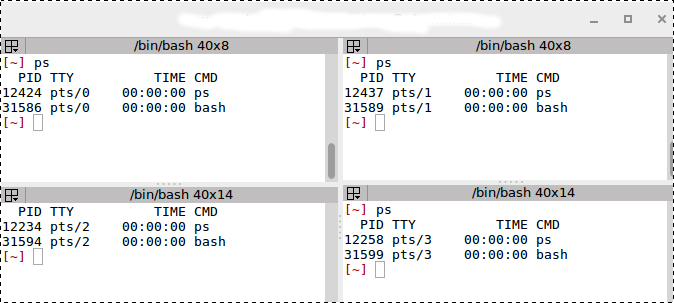
\includegraphics[width=1\textwidth]{figures/ps}\\
 
If you want this type of 2x2 layout, make a backup of \textsl{\ttb{}.config/terminator/config}. Next, recreate the \textsl{config} file with the following settings.\\
  
\begin{lstlisting}[escapeinside={¿}{¿},frame=single,breaklines]
  [global_config]
  enabled_plugins = CustomCommandsMenu, TestPlugin, TerminalShot, APTURLHandler, LaunchpadCodeURLHandler, LaunchpadBugURLHandler
  [keybindings]
  [layouts]
  [[default]]
  [[[child0]]]
  fullscreen = False
  last_active_term = c3520923-b680-4510-98c9-131e08a16f17
  last_active_window = True
  maximised = True
  order = 0
  parent = ""
  position = 0:27
  size = 1920, 986
  title = mgcr@LIB2015:~/.config/terminator
  type = Window
  [[[child1]]]
  order = 0
  parent = child0
  position = 958
  ratio = 0.500260416667
  type = HPaned
  [[[child2]]]
  order = 0
  parent = child1
  position = 489
  ratio = 0.498478701826
  type = VPaned
  [[[child5]]]
  order = 1
  parent = child1
  position = 489
  ratio = 0.498478701826
  type = VPaned
  [[[terminal3]]]
  order = 0
  parent = child2
  profile = default
  type = Terminal
  uuid = c3520923-b680-4510-98c9-131e08a16f17
  [[[terminal4]]]
  order = 1
  parent = child2
  profile = default
  type = Terminal
  uuid = c6dbb19a-0746-48ba-a9c5-576b6399243e
  [[[terminal6]]]
  order = 0
  parent = child5
  profile = default
  type = Terminal
  uuid = 6892246c-ee46-412a-82f9-ea15d0399865
  [[[terminal7]]]
  order = 1
  parent = child5
  profile = default
  type = Terminal
  uuid = 24723eb5-0621-4567-9305-ff7f8c3664c3
  # one is the old default			 
  [[one]]
  [[[child1]]]
  parent = window0
  type = Terminal
  [[[window0]]]
  parent = ""
  type = Window
  [plugins]
  [profiles]
  [[default]]
  background_image = None
  copy_on_selection = True
  scrollback_infinite = True	
  \end{lstlisting}
 
 For a quick look at other terminal emulators, please visit this URL: \href{https://opensource.com/life/15/11/top-open-source-terminal-emulators?sc\_cid=701600000011kF7AAI}{Top 7 open source terminal emulators}.

\subsection{controlling terminal IDs}

We can issue the command \tbi{stty -a} to find all the commands that help change and print terminal line settings. For example, we can see that \textasciicircum{}Z or CTRL+Z is used to suspend a running process in a termial window.\\

\begin{lstlisting}[escapeinside={¿}{¿},frame=single,breaklines]
¿\tld¿ stty -a
speed 38400 baud; rows 31; columns 117; line = 0; intr = ^C; quit = ^\; erase = ^?; kill = ^U; eof = ^D; eol = M-^?; eol2 = M-^?; swtch = M-^?; start = ^Q; stop = ^S; susp = ^Z; rprnt = ^R; werase = ^W; lnext = ^V; discard = ^O; min = 1; time = 0; -parenb -parodd -cmspar cs8 hupcl -cstopb cread -clocal -crtscts -ignbrk brkint -ignpar -parmrk -inpck -istrip -inlcr -igncr icrnl ixon -ixoff -iuclc ixany imaxbel iutf8 opost -olcuc -ocrnl onlcr -onocr -onlret -ofill -ofdel nl0 cr0 tab0 bs0 vt0 ff0 isig icanon iexten echo echoe echok -echonl -noflsh -xcase -tostop -echoprt echoctl echoke -extproc
\end{lstlisting}

\section {tty and pts}
For a quick discussion of \keyword{tty} and \keyword{pts}, read this URL: \href{http://unix.stackexchange.com/questions/93531/what-is-stored-in-dev-pts-files-and-can-we-open-them}{Stack Exchange}.

\begin{itemize}
\item \tbi{TTY} ports are usually direct connections to the computer such as a keyboard/mouse or a serial connection to the device. Old UNIX boxes would have dozens of of devices plugged into the back, all connected with cables. However, today system processes not initiated at a pseudo terminal slave are connected to a numbered tty: tty0, tty1, tty2

\item \tbi{PTS} stands for pseudo terminal slave. A terminal (or console) session needs one physical keyboard/screen combination that you sit and type at. However, from there you can create may pseudo terminal slave connections.  Remote SSH or telnet connections also initiate a pseudo terminal slave. Regardless, pseudo terminal slaves are numbered sequentially: pts/0, pts/1,...pts/n. In a way, pseudo terminal slaves are a virtual type of connection to the system.
\item \tbi{/DEV} Poke around in this folder and you will see that \keyword{tty} and \keyword{pts} files reside in this folder. \keyword{dev} is a special folder that contains device files for all devices. 
\end{itemize}

My observation is as follows:

\begin{enumerate}
	\item {Every process is connected to either a \emph{tty} or a \emph{pts}.} 
	\item {Processes connected to a \emph{tty} are started by the system or by a user from the desktop environment, i.e., launch the application using Gnome GUI menus.}
	\item {Processes connected to a \emph{pts} are started by a user at a terminal window, an ssh shell or simple bash terminal window.}
\end{enumerate}	

Ok, so let's list all of the processes running under the user \emph{mgcr}. Note that, in the code below, that I started the \keyword{ps} command at \emph{ps/0}, psuedo terminal slave 0, my first bash window. All other processes are connected to \emph{tty2}.  All other processes were either started by the system or started as a GUI application...such as \emph{texstudio} and \emph{chrome}.

\begin{lstlisting}[escapeinside={¿}{¿},frame=single,breaklines,columns=fixed,columns=fixed]	
¿\tld¿ ps -u mgcr | grep -E 'tty|pts'
5703   tty2     00:00:00 gvfsd-http
9535   tty2     00:00:36 texstudio
114271 tty2     00:00:00 evinced
21548  pts/0    00:00:00 ps
21549  pts/0    00:00:00 grep
.
.
24217  tty2     00:00:04 firefox
24569  tty2     00:11:12 opera:libflashp
24648  tty2     00:00:02 opera:libgnome-
#
# Note, when we pipe to grep, we loose our header. To get the header back, you can do the following. The first command up to the ';' prints the heading only. If you just issued the command 'ps -u mgcr', without the grep, you would also get the header information.
#
¿\tld¿ ps | head -1; ps -u mgcr | grep -E 'tty|pts'
   PID TTY      TIME     CMD
  5703 tty2     00:00:00 gvfsd-http
  9535 tty2     00:00:36 texstudio
114271 tty2     00:00:00 evinced
 21548 pts/0    00:00:00 ps
 21549 pts/0    00:00:00 grep
.
.
.
24217  tty2     00:00:04 firefox
24569  tty2     00:11:12 opera:libflashp
24648  tty2     00:00:02 opera:libgnome-
#
# So, we see that firefox is connected to tty2. I then closed firefox and started it (in the background with the command: firefox &)from the bash terminal . Note, it is now running as a pts/1 process where previously it ran at tty2.
#
¿\tld¿ firefox &
[1] 3571
¿\tld¿ ps -u mgcr | grep -E 'tty|pts' | grep firefox
3571 pts/1    00:00:05 firefox
#
# I closed firefox again, but this time I launched it from Gnome's Application Menu. Note, it is again running as a tty.
#
¿\tld¿ ps -u mgcr | grep -E 'tty|pts' | grep firefox
3849 tty2     00:00:05 firefox
\end{lstlisting}

\subsection{Be quiet, shh or is it ssh?}

Is it really that important to know to what type of terminal session a process is connected? Maybe and maybe not? For example, suppose I want to get a list of users who are remotely connected to my system using \keyword{ssh - secure shell}. In the example below, we see that one user is connected to our system using \emph{ssh} and that that connection is a psuedo terminal slave connection: \emph{pts/6}. What piece of information is more relevant, useful, or important? \tbi{Knowing} the terminal connection type? or \tbi{Knowing} who is connected and what type of connection protocol is being used?

\begin{lstlisting}[escapeinside={¿}{¿},frame=single,breaklines,columns=fixed]
#
# sshd is the secure shell daemon or process that permits users to remotely connect to a system using the ssh protocol.
#
# grep -v grep, just removes listing the grep command itself from the process list. Try the command without: grep -v grep.
#
# ps -aux, print a list of all user processes.
#	
¿\tld¿ ps -aux | grep -E 'tty|pts' | grep sshd | grep -v grep
mgc  6410  0.0  0.0 170796  4340 ?    S   08:52   0:00 sshd: mgc@pts/6
#
# Note: I grepped two things: terminal session type, tty or pts, and the sshd process. Let's remove the first grep that is grepping the termnal type.
#
¿\tld¿ ps -aux | grep sshd | grep -v grep
root 1558  0.0  0.0  81412  5772 ?    Ss   Jan17   0:00 /usr/sbin/sshd -D
root 6377  0.0  0.0 170796  9132 ?    Ss   08:52   0:00 sshd: mgd [priv]
mgc  6410  0.0  0.0 170796  4340 ?    S    08:52   0:00 sshd: mgd@pts/6
#
# So, we still get the sshd process connected to the pts, but we also get the main sshd process itself and a spawned sshd process started by user: mgc.
#
# grep is a very powerful tool that can help isolate information.  If you do not understand what you are doing, it can also easily hide information that may be relevant to your investigation.
#
# What if we wanted a bit more information about the remote connection?
#
# w = who is logged, what time did they connect, what are they doing?
#
# who = who is logged on, what date and time did they connect, and from where?
#
# w, tells us that user mgc started a pseudo teminal slave connection from a bash terminal, that started at 08:52, no other process has been started by: mgc.
#
# who, gives us similar information. User mgc started a pts connection, but in addition to time of day, we also get the date and more importantly the source IP address of the connection...which in this case is from another system on the local area network.
#
¿\tld¿ w | grep mgc
mgc      pts/6     08:52   32:12   0.02s  0.02s -bash

¿\tld¿ who | grep mgc
mgc      pts/6        2016-01-19 08:52 (192.168.0.18)
\end{lstlisting}

\begin{tabularx}{\linewidth}{>{\bfseries}X | X} % the X is needed to wrap text
\caption{Processes by Terminals}\label{table:processes-terminals}\\ % title of Table
\toprule
\normalfont{Command} & Action \\% inserts table heading, unbolds 1st column heading
\midrule
ps -ef grep -E \tqs{tty|pts} & full-format listing of all processes filtered on type of connection using grep's regex switch\\[2mm]
ps -ef grep \tqs{tty\textbackslash{}|pts} & full-format listing of all processes filtered on type of connection, regular grep with escape character before the \emph{logical or} symbol\\[2mm]
ps -ft pts/0 -t pts/2 -t tty1 & full-format listing of all processes on three terminals: pts/0, pts/2, and tty1\\[1mm]
ps -t pts/0 -t pts/2 -t tty1 & partial-format listing of all processes on three terminals: pts/0, pts/2, and tty1\\[1mm]
w & who is logged on and what are they doing,  a very condensed list, one per terminal\\[1mm]
who & who is logged on to terminals\\[1mm]
who am i & who am i (my user name) and on what terminal\\[1mm]
whoami & just show my user name\\[1mm]
\bottomrule
\end{tabularx}

\subsection{Horton the...}

Let's look at the \keyword{who} command in detail. Not only can we get information about users and terminal sessions, but we can also get information on the current run-level and the time and date of the last system boot.

\begin{lstlisting}[escapeinside={¿}{¿},frame=single,breaklines,columns=fixed]
#
# List the switches for the who command. Note, I am going to use the -H option often since I want to see the header.
#	
¿\tld¿ m- who # my .bashrc function 'm-'
-a, --all
-b, --boot
-d, --dead
-H, --heading 
-l, --login
--lookup
-m     only hostname and user associated with stdin
-p, --process
-q, --count
-r, --runlevel
-s, --short
-t, --time
-T, -w, --mesg
-u, --users
--message
--writable
--help display this help and exit
--version
#
# Let's start by getting just a list of logged on users, nothing else. The cut delimeter is a space. We want only the first field. We also want to sort this field and eliminate duplicates. We just want unique names. In this case '| uniq | sort' will also work. 
#
¿\color{red}{\textit{Be careful when using these two commands together: uniq and sort. If you don't get the result that you expect, try switching the order of the two commands.}}¿
#
¿\tld¿ who | cut -d' ' -f1 | sort | uniq
mgc
mgcr

#
# Who is logged on to terminal sessions? The options, -Hs and -T, would also produce the same output.
#
¿\tld¿ who -H
NAME LINE         TIME             COMMENT
mgcr tty2         2016-01-17 08:01 (:0)
mgcr pts/0        2016-01-17 08:01 (:0)
mgcr pts/1        2016-01-17 08:01 (:0)
mgcr pts/2        2016-01-17 08:01 (:0)
mgcr pts/3        2016-01-17 08:01 (:0)
mgc  pts/6        2016-01-19 08:52 (192.168.0.18)

#
# Get system boot time, runlevel, and terminal session info for all users.
#
¿\tld¿ who -Ha
NAME       LINE         TIME             IDLE          PID COMMENT  EXIT
           system boot  2016-01-17 19:54
           run-level 5  2016-01-17 19:55
           pts/0        2016-01-17 20:45              4524 id=ts/0  term=0 exit=0
mgcr + 	   tty2         2016-01-17 08:01  old        22295 (:0)
mgcr +     pts/0        2016-01-17 08:01 00:49       22797 (:0)
mgcr +     pts/1        2016-01-17 08:01 04:08       22797 (:0)
mgcr +     pts/2        2016-01-17 08:01   .         22797 (:0)
mgcr +     pts/3        2016-01-17 08:01 00:23       22797 (:0)
mgc      + pts/6        2016-01-19 08:52 04:51        6377 (172.18.0.18)
#
# Who is logged on at this terminal?
#
¿\tld¿ who -Hm
NAME     LINE         TIME             COMMENT
mgcr     pts/2        2016-01-17 08:01 (:0)
# 
# What is the run-level?
#
¿\tld¿ who -Hr
NAME     LINE         TIME             IDLE          PID COMMENT
         run-level 5  2016-01-17 19:55
#
# What users are logged on?
#
¿\tld¿ who -Hu
NAME LINE         TIME             IDLE          PID COMMENT
mgcr tty2         2016-01-17 08:01  old        22295 (:0)
mgcr pts/0        2016-01-17 08:01 00:04       22797 (:0)
mgcr pts/1        2016-01-17 08:01 04:18       22797 (:0)
mgcr pts/2        2016-01-17 08:01   .         22797 (:0)
mgcr pts/3        2016-01-17 08:01 00:32       22797 (:0)
mgc  pts/6        2016-01-19 08:52 05:01       6377 (192.168.0.18)

\end{lstlisting}

\subsection {Sending messages to users}
Ok, all well and nice, but how do we actually use all this information? A typical scenario is one where we need to reboot a server. Let's say we issued the \emph{who} command and saw that several users were connected. One by one, we could send a message to each user. In the following example, I am using my 2x2 terminal grid. I am going to send a message from my \emph{pts/0} terminal window to my \emph{pts/3} terminal window.

\begin{lstlisting}[escapeinside={¿}{¿},frame=single,breaklines]
#
# Sending from pts/0
#
¿\tld¿ who am i
mgcr pts/0        2016-01-17 08:01 (:0)
#
# After issuing the following command and hitting the enter key, you are taken to the next blank line. You then begin writing the message on consecutive lines or as one big line. Use CTRL+Z to end and send the message. Each time you hit the enter key, that line is sent to the other terminal.
#
¿\tld¿ write mgcr pts/3
hi there
system going down in 5 minutes...please close all applications and log off
^Z
[4]+  Stopped                 write mgcr pts/3
#
# An alternative to typing individual lines of the message followed CTRL+Z is to simply echo the information and pipe it to the write command.
#
¿\tld¿ echo "Hi, there! The system is going down in 5 minutes...time to panic!" | write mgcr pts/3
#
# What would I see on pts/3? I issue the 'who am i' command to show that I am on that terminal.
#
¿\tld¿ who am i
mgcr pts/3        2016-01-17 08:01 (:0)
#
# Then, immediatedly after I issue the write command on pts/0, this message appears...
#
¿\tld¿ 
Message from mgcr@LIB2015 on pts/0 at 14:05 ...
#
# And, as I type a line and hit the enter key, each line is displayed in succession. Unfortunately, at the destination prompt, there is no indication that more messages follow. The only way you know that there are no more messages is when you hit the enter key and are returned to the command prompt.
#
hi there
system going down in 5 minutes...please close all applications and log off
#
# Well, what if you had 100 users logged on? You certainly would not send 100 individual messages! You can instead use the wall command, which sends the same message to all users.
#
¿\tld¿ wall "system going down"

Broadcast message from mgcr@LIB2015 (pts/0) (Sun Jan 17 14:13:46 2016):  

system going down
#
# What would you see on each terminal window?
#
¿\tld¿
Broadcast message from mgcr@LIB2015 (pts/0) (Sun Jan 17 14:13:46 2016):  
system going down
#
# If you had a recurring event, you would want to send the same message each time. The best way to do this is to store your messages into files and then use standin to send the files to the wall command. Note, even the terminal session from which you send the message receives the message.
#
# The greater than symbol sends output or writes to the destination file: sgd.msg. The less than symbol sends the information the other direction. The contents of sgd.msg are sent to the wall command as input.
#
¿\tld¿ echo "system going down in 5 minutes...please close all applications and log off" > sgd.msg
¿\tld¿ wall < sgd.msg

Broadcast message from mgcr@LIB2015 (pts/0) (Sun Jan 17 14:27:27 2016):  

system going down in 5 minutes...please close all applications and log off   
#
# But, this just sends the message, it does not actually do anything about the reboot.
#
¿\tld¿ shutdown -r +15 "Server is going down in the middle of the day in order to create havoc and make you work less efficiently...all within the next 15 minutes. Please don't save ALL your work and do ignore this message!"  
#
# The above command schedules a system reboot in 15 minutes time and immediately sends out a message to all users logged onto the system.
#
\end{lstlisting}

In the above section, we used the \keyword{shutdown} command with its messaging feature. Please be aware that this method will not work for users at a different shell level than you and as well it will not send a message to users with a network connection such as: \tbi{ftp}, \tbi{smtp}, \tbi{pop3}, \tbi{tftp}, \tbi{ssh}. \textit{It is best to schedule shutdown and reboot times during a maintenance window that has been previously established and communicated to all users via email or some other messaging service.}

\section{Breaking a complex command into parts}

In the following table, I am just dabbling with the \keyword{w} command and showing how one can break a complex command into smaller steps. The web can be a great source of information and you will often find solutions to your problems or challenges. However, quite often the code in the solutions can be quit complex. \textit{I strongly recommend that you try to break the code down into its parts so that I understand each part.} I am going to illustrate this approach, but in reverse order. I start with a simple command and add more complex parts.

\begin{lstlisting}[escapeinside={¿}{¿},frame=single,breaklines,columns=fixed]
¿\tld¿ w
10:48:54 up 1 day, 14:54,  6 users,  load average: 3.69, 3.53, 3.39
USER TTY       LOGIN@  IDLE    JCPU   PCPU  WHAT
mgcr tty2      Mon08   38:54m  2days  0.04s opera:libflashp
mgcr pts/0     Mon08    2.00s  0.16s  0.00s w
mgcr pts/1     Mon08    1:13m  0.10s  0.10s /bin/bash
mgcr pts/2     Mon08    2:48m  0.06s  0.06s /bin/bash
mgcr pts/3     Mon08   10:54   0.14s  0.14s /bin/bash
mgc  pts/6     08:52    1:56m  0.02s  0.02s -bash
#
# Interesting...it looks like there are only 6 processes running, five for user mgcr on one for user mgc.
#
# Also, there is only one process on tty2. Is that correct? Let's use the ps command to list processes and filter on terminal tty2. We will also get a count of those processes on tty2.
# The first part of the command list our processes: ps -ft tty2
# The command separator is the semi-colon.
# The second part of the command pipes its output to 'wc -l', count the number of lines, the result is: 81.
#
# We use the ps command with the -f (full-format) and -t (terminal type) switches to get a list of only processes running on tty2.
#
¿\tld¿ ps -ft tty2 ; ps -ft tty2 | wc -l
UID   PID  PPID  C STIME TTY   TIME       CMD
mgcr  2146    1  0 Jan18 tty2  00:00:24   javaws.itweb -splash:/usr/share/icedtea-web/javaws_splash.png -Xbootc
mgcr  2212 2146 99 Jan18 tty2  1-09:26:52 javaws.itweb -splash:/usr/share/icedtea-web/javaws_splash.png -Xboo
.
.
mgcr 29929 22805 3 11:09 tty2  00:00:00   [opera:libflashp] <defunct>
81
¿\tld¿
#
# So, removing the line count for the heading, mgcr has 80 processes running on tty2. I elided most of the process listing which is indicated by the two vertical periods.
#
# Ok, what we eventually want to do is to loop through each terminal type in order to see the running processes for each terminal type. We begin by using the output of the w command to get a simple list of all terminal types, which is listed in column 2 of the output of this command. We use awk to isolate column 2, represented by {print $2}.
#
¿\tld¿ w | awk '{print $2}'
up
TTY
tty2
pts/0
pts/1
pts/2
pts/3
pts/6
# 
# We need to get rid of the first two rows. Why? Drop the pipe to see full output of w. As above, we only want the second column. We use 'grep -v', inverse grep, to remove the two lines. That is the lines containing: up or TTY. Another option to remove the two lines would be to use the sed command. ¿\textbf{\color{red}Challenge:} How would you do that? \hyperlink{sedel}{Answer.}¿
#
¿\tld¿ w | awk '{print $2}' | grep -v "up\|TTY"
tty2
pts/0
pts/1
pts/2
pts/3
pts/6
#
# Alright, now let's loop through all these terminals.
#
¿\tld¿ for trm in `w | awk '{print $2}' | grep -v "up\|TTY"`; do ps -ft $trm;done
¿\textbf{\color{red}UID        PID  PPID  C STIME TTY          TIME CMD}¿
mgcr 2146     1  0 Jan18 tty2  00:00:25  javaws.itweb -splash:/usr/share/icedtea-web/javaws_splash.png -Xbootc
mgcr 2212  2146 99 Jan18 tty2  -10:07:16 javaws.itweb -splash:/usr/share/icedtea-web/javaws_splash.png -Xboo
.
.
mgcr 32307 31952  0 11:21 tty2     00:00:00 /opt/google/chrome/chrome --type=renderer --lang=en-GB --force-fieldt
¿\textbf{\color{red}UID        PID  PPID  C STIME TTY          TIME CMD}¿
mgcr  2592 23027  0 11:34 pts/0    00:00:00 ps -ft pts/0
mgcr 23027 22797  0 Jan18 pts/0    00:00:00 /bin/bash
¿\textbf{\color{red}UID        PID  PPID  C STIME TTY          TIME CMD}¿
mgcr 23030 22797  0 Jan18 pts/1    00:00:00 /bin/bash
¿\textbf{\color{red}UID        PID  PPID  C STIME TTY          TIME CMD}¿
mgcr 23035 22797  0 Jan18 pts/2    00:00:00 /bin/bash
¿\textbf{\color{red}UID        PID  PPID  C STIME TTY          TIME CMD}¿
mgcr 23040 22797  0 Jan18 pts/3    00:00:00 /bin/bash
¿\textbf{\color{red}UID        PID  PPID  C STIME TTY          TIME CMD}¿
mgc       6421  6410  0 08:52 pts/6    00:00:00 -bash
#
# Ugh, note, it prints the heading at the beginning of each terminal type...let's remove the heading using the --no-heading switch for ps.
#
¿\tld¿ for trm in `w | awk '{print $2}' | grep -v "up\|TTY"`; do ps --no-heading -ft $trm;done
mgcr  2146     1  0 Jan18 tty2     00:00:25 javaws.itweb -splash:/usr/share/icedtea-web/javaws_splash.png -Xbootc
mgcr  2212  2146 99 Jan18 tty2     1-10:11:26 javaws.itweb -splash:/usr/share/icedtea-web/javaws_splash.png -Xboo
.
.
mgcr 32307 31952  0 11:21 tty2     00:00:00 /opt/google/chrome/chrome --type=renderer --lang=en-GB --force-fieldt
mgcr  2968 23027  0 11:36 pts/0    00:00:00 ps --no-heading -ft pts/0
mgcr 23027 22797  0 Jan18 pts/0    00:00:00 /bin/bash
mgcr 23030 22797  0 Jan18 pts/1    00:00:00 /bin/bash
mgcr 23035 22797  0 Jan18 pts/2    00:00:00 /bin/bash
mgcr 23040 22797  0 Jan18 pts/3    00:00:00 /bin/bash
mgc   6421  6410  0 08:52 pts/6    00:00:00 -bash
#
# As an aside, I noticed that mgcr and mgd did not have any processes on tty1.  Who does? It turns out that only the user with UID gdm, the GNOME Display Manager, has processes on that terminal.
#
¿\tld¿ ps -ft tty1
UID  PID  PPID  C STIME TTY      TIME     CMD
gdm  1671 1609  0 Jan17 tty1     00:00:00 /usr/libexec/gdm-wayland-session /usr/bin/gnome-session --autostart /
.
.
.
gdm       2072  1943  0 Jan17 tty1     00:00:00 /usr/libexec/ibus-engine-simple
\end{lstlisting}

So, typically you may find a complex command on the Internet such as this command...

\begin{lstlisting}[escapeinside={¿}{¿},frame=single,breaklines,columns=fixed]
for trm in `w | awk '{print $2}' | grep -v "up\|TTY"`; do ps --no-heading -ft $trm;done
\end{lstlisting}

Your task would be to break down this command into its smaller parts, the reverse of what I did in building up to my final command. This is a tremendous way of learning! \textit{Don't just find and use commands without fully understanding  what they do.} You will quickly advance your learning and skill set if you dissect complex commands you find on the Internet.

\subsection{How to get just one header}

Ok, what if we wanted only that initial heading? Here is some code that will print the heading once and only once. It uses a counter called \emph{count} and a \emph{for} loop. The header is printed on the first iteration through the loop when count=1. Save this file as \textsl{pts.sh} and then \emph{chmod u+x pts.sh} to make it executable. To run the code, type: \emph{bash pts.sh} or \emph{./pts.sh}. You will get a list of all processes sorted by terminal type with the heading only at the beginning of the output.

\begin{lstlisting}[escapeinside={¿}{¿},frame=single,breaklines]
¿\tbi{\#}¿/bin/bash
# Print heading only on first iteration through the loop.
count=0
for trm in `w | awk '{print $2}' | grep -v "up\|TTY"`
do
#
# Note: the counter statement uses (( ... )) but the 'if' statement uses [[ ... ]]. Also, pay attention to the spaces inside the curved and square brackets.
#
(( count++ ))    
if [[ $count -eq 1 ]]
then
ps -ft $trm
else
ps --no-heading -ft $trm
fi
done
\end{lstlisting}

\section{User processes}

Let's return to the \keyword{sleep} command. I am logged on as user \emph{mgcr}. When I issue just the \keyword{ps} command, I am only getting the processes for the pseudo terminal session. What about the processes for \emph{mgcr}?

\begin{lstlisting}[escapeinside={¿}{¿},frame=single,breaklines,columns=fixed]
¿\tld¿ (sleep 60 ; echo "meme" > ./sleepy) &
[1] 19967

¿\tld¿ ps
PID   TTY      TIME     CMD
14821 pts/1    00:00:00 bash
19967 pts/1    00:00:00 bash
19969 pts/1    00:00:00 sleep
19977 pts/1    00:00:00 ps
#
# Is the sleep process one of mine?
#
¿\tld¿ ps -u mgcr | grep sleep
19969 pts/1    00:00:00 sleep
#
# After 60 seconds, let's grep for "echo"...we could have also grepped for "sleep".
#
¿\tld¿ ps -u mgcr | grep echo
[1]+  Done                    ( sleep 60; echo "meme" > ./sleepy )	
\end{lstlisting}

\subsection{User processes - splitting hairs}
As above, we can get a list of all processes for a specific user. In the code below, I issue the \emph{ps -u mgcr} command to get a list of all processes started by the user \emph{mgcr}. In the following examples, I give only a snippet of the process list. As you can see, mgcr appears that we have 113 processes running. But, do we really?

\begin{lstlisting}[escapeinside={¿}{¿},frame=single,breaklines,columns=fixed]
¿\tld¿ whoami
mgcr
	
¿\tld¿ ps -u mgcr
PID  TTY      TIME     CMD
2176 ?        00:00:00 systemd
2177 ?        00:00:00 (sd-pam)
.
.
28392 tty2    00:00:13 evince
28399 tty2    00:00:00 evinced
#
# wc -l = print the newline counts
#
¿\tld¿ ps -u mgcr | wc -l
113
#
# But, this is rather cumbersome...we are using two commands; one to get a list of the processes and another to get a count of the running processes.
#
# Alternatively, we can pipe our output to bash's nl command in order to prepend the line number of each line. Note: piping to 'cat -n' will give the same result.
#
# We have to subtract one from the result because our count includes the heading. So, it looks like mgcr has 113 processes running, not 114.
#
¿\tld¿ ps -u mgcr | nl
1 PID     TTY      TIME     CMD
2 2176    ?        00:00:00 systemd
3 2177    ?        00:00:00 (sd-pam)
.
.
113 28392 tty2     00:00:13 evince
114 28399 tty2     00:00:00 evinced
#
# Let's try stripping the heading from our list. Below, I illustrate three ways of doing this. Only use one of these methods at a time.
#
¿\tld¿ ps -u mgcr | awk '{if(NR>1)print}' | nl
¿\tld¿ ps -u mgcr | sed -n '1!p' | nl
¿\tld¿ ps -u mgcr | tail -n +2 | nl
#
# All three of these commands produce the following listing...
#
1 2176    ?        00:00:00 systemd
2 2177    ?        00:00:00 (sd-pam)
.
.
113 28392 tty2     00:00:13 evince
114 28399 tty2     00:00:00 evinced
#
# Why is the count not 113?
#
# Answer: Each solution pipes to an additional command: awk, or sed, or tail. So, we are adding one additional process and removing the heading...which balances out. Just remember that when you issue a pipe, you are adding a process. 
#
# So, is the number of running processes 113?
#
# The number of running processes is actually 110! ¿\textbf{\color{red}Say, what?}¿
#
# To get our actual count of the total number of running processes, we have to remove the count for the heading, the count for 'wc -l' itself, and the count for 'ps -u mgcr'.
#
# Interesting or totally irrelevant? Hmmm...
#
\end{lstlisting}

\subsection{Counting user processes - the Harley metric}

There is an easy way to find out the number of user processes for each user on a system. These metrics may be helpful if your system is bogging down and you want a quick check to find the \tbi{hog} of all your system resources. I present the command and then create an alias called \emph{hog}. Trust me, you will often use this alias.

\begin{lstlisting}[escapeinside={¿}{¿},frame=single,breaklines]
#
# Note: 'sort' before 'uniq'...go ahead and try it the other way! Only two columns of information are generated: total user processes and user name.
#
¿\tld¿ ps -eo user=|sort|uniq -c
2 avahi
1 chrony
1 colord
1 dbus
25 gdm
1 lp
4 mgd
126 mgcr
1 nobody
1 polkitd
1 qemu
173 root
1 rtkit
#
# Hmm, the above command sorted by user name. Let's sort by descending order of the count.  -n=numeric, -r=reverse
#
¿\tld¿ ps -eo user=|sort|uniq -c | sort -n -r
174 root
127 mgcr
25 gdm
4 mgd
2 avahi
1 rtkit
1 qemu
1 polkitd
1 nobody
1 lp
1 dbus
1 colord
1 chrony
#
# You expect me to remember that command? Ok, let's create a command alias and add it to our .bashrc file. Pay attention to the different types of quotations that are used! We then just call the function by typing hog...after we have sourced .bashrc.
#
¿\tld¿ echo "alias hog='ps -eo user=|sort|uniq -c | sort -n -r'">>~/.bashrc

¿\tld¿ tail -1 ~/.bashrc
alias hog='ps -eo user=|sort|uniq -c | sort -n -r'

¿\tld¿ hog
174 root
127 mgcr
25 gdm
4 mgd
2 avahi
1 rtkit
1 qemu
1 polkitd
1 nobody
1 lp
1 dbus
1 colord
1 chrony

\end{lstlisting}

\section{Filtering process information}

\subsection{Introduction}

The simple \keyword{ps} command provides a ton of information. You will definitely want to read the manpage for \emph{ps} as there are many command switches and options that help to isolate and filter the information.

\subsection{ps switches/options explained} 

For the next discussion of \keyword{ps}, I want to use some specific switches that allow us to see all running processes.

\begin{itemize}
	\item[] \tbi{-A }Select all processes. Identical to -e.
	\item[] \tbi{-e }Select all processes. Identical to -A. 
	\item[] \tbi{-a }All processes except both session leaders (see getsid(2)) and processes not associated
	\item[] \tbi{-f }  Do full-format listing.
	\item[] \tbi{-o } Format, i.e., options, what to print.  
\end{itemize}

\subsection{examples of ps switch/options - filtering process fields}

\begin{lstlisting}[escapeinside={¿}{¿},frame=single,breaklines,columns=fixed]
#
# If you recall from the start of this chapter, the ps command by itself just presents process info for the bash terminal window.
#
¿\tld¿ ps
PID   TTY      TIME     CMD
7770  pts/3    00:00:00 ps
23040 pts/3    00:00:00 bash
#
# Let's get a count of all running processes.
#
¿\tld¿ ps aux | wc -l
333
#
# We can also use the -ef switch. Note, there is a small difference in the count.
#
¿\tld¿ ps -ef | wc -l
336
#
# We can also use the -Af switch.
#
¿\tld¿ ps -Af | wc -l
336
#
# Suppose I wanted a count of just the process containing the string "gdm"?
#
¿\tld¿ ps -ef | grep gdm | wc -l
31
#
# Ok, let's just list the 1st four of those processes.
#
¿\tld¿ ps -ef | head -4 | grep gdm
¿\tld¿ 
#
# Hmm, nothing was returned. Why? The order of the piping was incorrect. I asked to filter the first full lines of the output. But, in that output, no line contained "gdm". Therefore, the second pipe 'grep gdm' returned nothing. Switch the order. Put the head statement after the grep statement.
#
¿\tld¿ ps -ef | grep gdm | head -4
root  1579     1  0 Jan17 ?     00:00:00 /usr/sbin/gdm
root  1609  1579  0 Jan17 ?     00:00:00 gdm-session-worker [pam/gdm-launch-environment]
gdm   1630     1  0 Jan17 ?     00:00:00 /usr/lib/systemd/systemd --user
gdm   1632  1630  0 Jan17 ?     00:00:00 (sd-pam)
#
# Note two things from the above output. The string "gdm" was under both the UID and CMD column headers. How do I know these column headers?
#
¿\tld¿ ps -ef | head -1
UID        PID  PPID  C STIME TTY          TIME CMD
#
# So, how do I get the column header as well as the process information? And, just display the UID and CMD columns? I am going to use the awk's 'Output Field Separator=OFS' switch with the OFS equal to a tab, \t. To get the UID and CMD headers only, I know that I need to print only columns 1 and 8. 
#
¿\tld¿ ps -ef | head -1 | awk -v OFS='\t' '{print $1,  $8}'
UID		CMD
#
# Ok, that prints the heading. We just need to add the command to grep "gdm" and display only the first 4 lines of process information.
#
¿\tld¿ ps -ef | head -1 | awk -v OFS='\t' '{print $1,  $8}' ; ps -ef | grep gdm | head -4 | awk -v OFS='\t' '{print $1, $8}'
UID¿\qquad¿CMD
root¿\qquad¿/usr/sbin/gdm
root¿\qquad¿gdm-session-worker
gdm¿\qquad¿/usr/lib/systemd/systemd
gdm¿\qquad¿(sd-pam)
#
# Pretty cool! Is this command another candidate for a function?
#
# Here are some variations on awk formatting. In the first command, I am putting a fixed 5 spaces between the double-quotations. In the second command,I am using \t for one tab...which by default equals 5 spaces.
#
¿\tld¿ ps -ef | head -1 | awk '{print $1 "     " $8}'
UID¿\qquad¿CMD

¿\tld¿ ps -ef | head -1 | awk '{print $1 "\t" $8}'
UID¿\qquad¿CMD
#
# We can also get the same information with the 'ps aux' command. Here, I want the 1st and 11th column headers and the first 4 processes in the process list.
#
¿\tld¿ ps aux | awk '{print $1, $11}' | head -4
USER COMMAND
root /usr/lib/systemd/systemd
root [kthreadd]
root [ksoftirqd/0]
#
# And, of course, as soon as we grep, we loose our heading.
#
¿\tld¿ ps aux | awk '{print $1, $11}' | grep gdm | head -4
root /usr/sbin/gdm
root gdm-session-worker
gdm /usr/lib/systemd/systemd
gdm (sd-pam)
#
# Let's tet the heading back.
#
¿\tld¿ ps aux | awk '{print $1, $11}' | head -1 ; ps aux | awk '{print $1, $11}' | grep gdm | head -4
USER COMMAND
root /usr/sbin/gdm
root gdm-session-worker
gdm /usr/lib/systemd/systemd
gdm (sd-pam)
#
# Let's format the output a little differently...using tabs and pipe to less so that we can page through the screens of information. Hit the q key to quit the less pager.
#
¿\tld¿ ps aux | awk '{print $1, "\t", $2, "\t", $10, "\t", $11}' | less
USER     PID     TIME    COMMAND
root     1       0:02    /usr/lib/systemd/systemd
root     2       0:00    [kthreadd]
.
.
root     31      0:00    [kworker/3:0H]
root     32      0:05    [rcuos/3]
:
#
# Come on, there must be an easier way, awk seems so cumbersome?
#
# How about just printing four of the gdm processes and only output the pid and cmd fields? Really, can we call the fields by name?
#
¿\tld¿ ps -eo pid,cmd | grep gdm | head -4
1579 /usr/sbin/gdm
1609 gdm-session-worker [pam/gdm-launch-environment]
1671 /usr/libexec/gdm-wayland-session /usr/bin/gnome-session --autostart /usr/share/gdm/greeter/autostart  --session gnome-wayland
1705 /usr/libexec/gnome-session-binary --autostart /usr/share/gdm/greeter/autostart --session gnome-wayland
#
# It gets really tricky once you start playing with ps options.
#
¿\tld¿ ps -ef | head -2
UID        PID  PPID  C STIME TTY TIME     CMD
root         1     0  0 Jan17 ?   00:00:28 /usr/lib/systemd/systemd --switched-root --system --deserialize 21
#
# Alright, let's just get the UID and PID columns
#
¿\tld¿ ps -eo uid,pid | head -2
UID   PID
0     1
#
# Ok, no problem there, the output is consistent.
#
¿\tld¿ ps -efo uid,pid | head -2
UID        PID
1858215107 22295
#
# Just a sec, I simply added the full-format switch and now my UID is 1858215107.
#
¿\tld¿ id -u root
0
¿\tld¿ id -u mgcr
1858215107
# 
# So, with just the -eo switch, the first processes listed are for root whose UID is 0. With -efo, the first processes listed are for mgcr, the user that is logged on. Note: this value is the EUID system variable, the effective user ID.
#
¿\tld¿ ps -efo uid,pid  | grep gdm | head -2
¿\tld¿
#
# Hey, nothing was returned...after digging a little deeper in the man page...
#
¿\tld¿ ps -eo ruser=RealUser -o pid  | grep gdm | head -2
gdm       1630
gdm       1632
#
# Awesome, how about the header?
#
¿\tld¿ ps -eo uid,pid | head -1; ps -eo ruser=RealUser -o pid  | grep gdm | head -2
UID   PID
gdm   1630
gdm   1632
¿\tld¿ 
\end{lstlisting}

\subsection{AIX Format Descriptors (and making an alias out of a function)}

The \keyword{AIX FORMAT DESCRIPTORS} section of the \keyword{ps} manpage provides useful information about headers that we can use in our \emph{ps} commands. Until you can remember all these descriptors, you will want a quick way to display them. We can display the descriptors using my \emph{.bashrc mang} function. However, even this would be cumbersome to type each time you wanted to display the descriptors. How about creating an alias from a specific use of the \emph{mang} function. As the manpage describes, we can use any of the following descriptors: \emph{code, normal, header}.


\begin{lstlisting}[escapeinside={¿}{¿},frame=single,breaklines,columns=fixed]
#
# Here is my 'mang' function...
#
¿\tld¿ grep -A12 "function mang" .bashrc
function mang()
#
# This is another way of printing a section of a manpage.
# Change section headers to uppercase using echo and tr.
# Use the A (after) and B (before) grep switches with large values that ensure we just capture the section.
# $1 = manpage $2 = first header and $3 = second header
# Example: mang sed name synopsis
# 
{
b=`echo $2 | tr '[a-z]' '[A-Z]'`
e=`echo $3 | tr '[a-z]' '[A-Z]'`
man $1 | col -b| grep -A1000 -x "$b" | grep -B1000 -x "$e" | sed '$d'
}
#
# So, let's use my mang function to print the aix format descriptors section of the ps manpage
#
¿\tld¿ mang ps "aix format descriptors" "standard format specifiers"
AIX FORMAT DESCRIPTORS
This ps supports AIX format descriptors, which work somewhat like the formatting codes of printf(1) and  printf(3).  For example, the normal default output can be produced with this: ps -eo "%p %y %x %c".  The NORMAL codes are described in the next section.

CODE   NORMAL   HEADER
%C     pcpu     %CPU
%G     group    GROUP
%P     ppid     PPID
%U     user     USER
%a     args     COMMAND
%c     comm     COMMAND
%g     rgroup   RGROUP
%n     nice     NI
%p     pid      PID
%r     pgid     PGID
%t     etime    ELAPSED
%u     ruser    RUSER
%x     time     TIME
%y     tty      TTY
%z     vsz      VSZ
¿\tld¿
#
# Ok, let's create an alias out of this specific mang function and append it to the end of my .bashrc file. We are going to create an alias called: aix.
#	
¿\tld¿ echo "alias aix='mang ps "aix format descriptors" "standard format specifiers"'" >>.bashrc
#
# I can issue the 'source .bashrc' command to re-read my .bashrc file.
#
¿\tld¿ source .bashrc

¿\tld¿ aix
AIX FORMAT DESCRIPTORS
This ps supports AIX format descriptors, which work somewhat like the formatting codes of printf(1) and printf(3).  For example, the normal default output can be produced with this: ps -eo "%p %y %x %c".  The NORMAL codes are described in the next section.

CODE   NORMAL   HEADER
%C     pcpu     %CPU
%G     group    GROUP
%P     ppid     PPID
%U     user     USER
%a     args     COMMAND
%c     comm     COMMAND
%g     rgroup   RGROUP
%n     nice     NI
%p     pid      PID
%r     pgid     PGID
%t     etime    ELAPSED
%u     ruser    RUSER
%x     time     TIME
%y     tty      TTY
%z     vsz      VSZ
\end{lstlisting}

Ok, le's start using the different \keyword{aix} descriptors in our \keyword{ps} commands. Obviously, we only need our \keyword{aix} function to call up our table whenever we want to see the full \keyword{AIX FORMAT DESCRIPTORS} list.

\begin{lstlisting}[escapeinside={¿}{¿},frame=single,breaklines,columns=fixed]
#
¿\tld¿ ps -eo "%U %p %C" | head -3
USER 	PID %CPU
root 	1    0.0
root 	2    0.0
#
# There is an alternative to the above command where we drop the parentheses. There is no space between each code descriptor. If you put a space without the double-quotations, you would get an error message. Notice that 'head -3' includes the header as one component of the list.
#
¿\tld¿ ps -eo %U%p%C | head -3
USER       PID %CPU
root         1  0.0
root         2  0.0
#
# Using the normal descriptors.
#
¿\tld¿ ps -eo user,pid,pcpu | head -3
USER       PID %CPU
root         1  0.0
root         2  0.0
#
# Ok, let's do some sorting. We are going to display the ruser, pid, and nice values. Note, only when we sort on column 2 do we get the header.
# sort options: -n = numeric sort, -nr = reverse numeric sort, -k = sort to column
#
¿\tld¿ ps -eo %u%p%n | sort -n -k 2 | head -6
RUSER      PID  NI
root         1   0
root         2   0
root         3   0
root         4   0
root         5 -20
#
# Let's sort on column 1, the real user name.
#
¿\tld¿ ps -eo %u%p%n | sort -n -k 1 | head -6
avahi      945   0
avahi      959   0
chrony     924   0
colord    1593   0
dbus       917   0
gdm       1632   0
#
# Let's sort on column 3, the nice value.
#
¿\tld¿ ps -eo %u%p%n | sort -n -k 3 | head -6
root       101 -20
root       103 -20
root       108 -20
root       110 -20
root       111 -20
root       144 -20
#
# Let's do a reverse sort on column 3, largest to smallest nice value.
#
¿\tld¿ ps -eo %u%p%n | sort -nr -k 3 | head -6
root       904  19
root        39  19
mgcr 	  2855  19
mgcr      2820  19
root        38   5
rtkit      908   1
#
# A bit of cheese and whine..but, I want the headers...
#
¿\tld¿ ps -eo %u%p%n | head -1 ; ps -eo %u%p%n | sort -nr -k 3 | head -6
RUSER      PID  NI
root       905  19
root        39  19
mgcr      2813  19
mgcr      2800  19
root        38   5
rtkit      906   1
#
# Hey, hey, did you see that? I got all top 6 processes that I requested not header plus 5 processes. Do I focus on detail? Maybe! Have I asked that question before? Maybe!
#
\end{lstlisting}

\section{Finding top consumers of computer resources}\label{sec:topcpu}

At the most inconvenient of times, servers will start to bog down as they run out of computing resources. We already covered how to find users who are running the most number of processes. We can also do a search to find the top processes that are consuming CPU and Memory resources.

\begin{lstlisting}[escapeinside={¿}{¿},frame=single,breaklines,columns=fixed]
#
# Let's sort by descending order of memory usage.
#
¿\tld¿ ps -eo pid,uname,cmd,pmem,pcpu --sort=-pmem | head -5
PID   USER  CMD                         %MEM %CPU
12745 qemu  /usr/bin/qemu-system-x86_64 26.1 12.4
3849  mgcr  /usr/lib64/firefox/firefox   3.3  2.3
2212  mgcr  javaws.itweb -splash:/usr/s  2.9  160
22805 mgcr  /usr/lib64/opera/opera       2.2 19.5
#
# Let's now sort by descending CPU usage.
#
¿\tld¿ ps -eo pid,uname,cmd,pmem,pcpu --sort=-pcpu | head -5
PID   USER  CMD                         %MEM %CPU
2212  mgcr  javaws.itweb -splash:/usr/s  2.9  160
22307 mgcr  /usr/libexec/Xorg vt2 -disp  1.1 61.4
16255 mgcr  /opt/google/chrome/chrome -  1.1 26.1
22805 mgcr  /usr/lib64/opera/opera       2.2 19.5
#
# Ok, let's use a slightly different approach...this comand was issued a bit later so the process data is slightly different.
#
¿\tld¿ ps axo pid,args,pmem,rss,vsz --sort -pmem,-rss,-vsz | head -n 5
PID  COMMAND                     %MEM    RSS     VSZ
2951 /usr/lib64/firefox/firefox   2.5 623112 2491152
2828 /usr/lib64/opera/opera       2.0 492420 1356268
2615 /usr/bin/gnome-shell         1.5 372808 2391872
3524 /opt/google/chrome/chrome -  1.5 370540 1370892
#
# Suppose we want a real-time monitor running in one of our bash windows that would update every 10 seconds. To do this we use the watch command.
#
¿\tld¿ watch -n 10 'ps -eo pid,uname,cmd,pmem,pcpu --sort=-pcpu | head -5'
Every 10.0s: ps -eo pid,uname,cmd,pmem,pcpu --sort=-pcpu | head -5                           Thu Jan 21 08:47:32 2016

PID  USER  CMD                         %MEM %CPU
2782 mgcr  /usr/lib64/opera/opera       1.8 14.0
4680 mgcr  /usr/lib64/opera/pluginwrap  0.5  3.2
2565 mgcr  /usr/bin/gnome-shell         1.5  3.0
2878 mgcr  /usr/lib64/firefox/firefox   1.2  2.6
#
# This information would refresh every 10 seconds. CTRL+C to end.
#
\end{lstlisting}

\section{pids}

\subsection{Introduction}

Every process or application that is started is assigned a unique \emph{process id} or \emph{pid}. 

\subsection{Working with PIDs}

\begin{lstlisting}[escapeinside={¿}{¿},frame=single,breaklines,columns=fixed]
#
# Display the last 10 processes in our process list.
#
~] ps aux | tail -10
mgcr 14803  0.3  0.1 962800 37116 tty2     Sl+  08:46   0:00 /usr/bin/gedit
root 14818  0.0  0.0      0     0 ?        S    08:46   0:00 [kworker/1:3]
.
.
mgcr 15930  0.0  0.0 112208  1804 pts/2    S+   08:50   0:00 tail -10
#
# Let's just display the full-format PID information for two of these processes by specifying their PIDs.
#
¿\tld¿ ps -fp 14803,14818
UID   PID    PPID  C STIME TTY    TIME     CMD
mgcr  14803     1  0 08:46 tty2   00:00:00 /usr/bin/gedit
root  14818     2  0 08:46 ?      00:00:00 [kworker/1:3]
#
# Each running process has a directory in the /proc directory. Inside this process directory, there are a large number of files related to the process.
#
¿\tld¿ man proc | grep -x DESCRIPTION -A3
DESCRIPTION
The  proc  filesystem  is a pseudo-filesystem which provides an interface to kernel data structures.  It is commonly mounted at /proc.  Most of it is read-only, but some files allow kernel variables to be changed.
# 
# Ok, let's take a peek at the files for the process with PID 14803. Let's do a long-listing first.
#
¿\tld¿ ls -la /proc | grep 14803
dr-xr-xr-x.   9 me mygrp               0 Jan 21 08:46 14803
#
# How many files/folders? As you can see this PID has 728 files associated with it...some within subfolders of the 14803 directory.
#
¿\tld¿ find /proc/14803 -type f | wc -l
728
#
# We can get limited information about a process using just the ps command followed by a process ID.
#
¿\tld¿ ps 32503
PID 	TTY      STAT   TIME COMMAND
32503 	?        S      0:00 [kworker/0:3]
#
# However, if we add the u option, more information is provided.
#
¿\tld¿ ps u 32503
USER       PID %CPU %MEM    VSZ   RSS TTY   STAT START   TIME COMMAND
root     32503  0.0  0.0      0     0 ?     S    14:04   0:00 [kworker/0:3]
\end{lstlisting}	

\section{Killing Processes}

\subsection{Introduction}

So, what happens when we have a runaway process that is out of control and eating up available CPU and memory resources? We have to end or kill that process.

\subsection{Using \emph{yes} and \emph{sleep} to test running processes}

In the following examples, I am going to make use of the \keyword{yes} command. If you type this command at the console, an endless stream of \emph{y's} will appear at the console. The \emph{yes} command may not make a lot of sense, but it is commonly used if you need to pipe the \emph{yes} string "y" to another command in order to answer positively yes to a series of questions...such as during installation of a program.

I am also going to start the \emph{yes} program in the \emph{background} and redirect the standard output of \emph{yes} to \textsl{/dev/null}. Any data sent to \textsl{/dev/null} disappears, it acts as a black hole.

Similarly, I am going to run the \keyword{sleep} command in the background.

Manapge description of \emph{yes}: output a string repeatedly until killed.

Manpage description of \emph{sleep}: delay for a specified amount of time.

\begin{lstlisting}[escapeinside={¿}{¿},frame=single,breaklines,columns=fixed]
#
# Send all the y lines to the blackhole and run the process in the background.
#
¿\tld¿ yes > /dev/null &
[1] 27955
#
# Get the pid of the yes command.
#
¿\tld¿ ps h -o pid -C yes
27955
#
# Note: the h option says: no header.
#
¿\tld¿ ps -o pid -C yes
PID
27955
#
# Another way to get the pid of the command: yes.
#
¿\tld¿ pidof yes
27955
#
# Yet another way of getting the pid value of yes.
#
¿\tld¿ pgrep yes
27955
#
# Let's get a bit more information on yes. I want the pid, nice, and command fields.
#
¿\tld¿ ps -eo pid,nice,command | grep yes | grep -v grep
27955   0 yes
#
# Ok, yes, it is time to kill yes...using command redirection.

¿\tld¿ kill -9 `(pidof yes)`
[1]+  Killed                  yes > /dev/null
#
# Is it killed? Yes, yes no longer exists.
#
¿\tld¿ pgrep yes
¿\tld¿
#
# Start it again...
#
¿\tld¿ yes > /dev/null &
[1] 32597
#
# Let's start another job, this time using the sleep command...sleep for 100 seconds.
#
¿\tld¿ sleep 100 &
[2] 19754
#
# What are the running jobs in this bash terminal?
#
¿\tld¿ jobs
[1]+  Running                 yes > /dev/null &
[2]+  Running                 sleep 100 &
#
# What are the pid values of yes and sleep?
#
¿\tld¿ pidof yes
32597

¿\tld¿ pidof yes
19754
#
# Let's kill both these processes, but this time let's use the job numbers. Note, job numbers are static until they are terminated. When I kill job 1, job 2 does not become job 1, it stays numbered as 2. See kill's manpage for the different kill options.
#
¿\tld¿ kill %1
[1]+  Terminated              yes > /dev/null

¿\tld¿ jobs
[2]+  Running                 sleep 100 &

¿\tld¿ kill -9 %2
[2]+  Killed                  sleep 100
#
# Let'start yes again.
#
¿\tld¿ yes > /dev/null &
[1] 313
#
# Ok, yes started again and its job number is still 1.
#
¿\tld¿ jobs
[1]+  Running                 yes > /dev/null &
#
# Let's check two variables: pts and SHLVL
#
¿\tld¿ who -m
mgcr pts/1        2016-01-21 07:49 (:0)

¿\tld¿ echo $SHLVL
2
#
# Let's open a new bash terminal by issuing  the bash command. We could also have just switched to an existing bash terminal window.
#
¿\tld¿ bash
#
# Note, my command prompt changed, I am still in the same bash terminal, pts/1, but the shell level, SHLVL, is now 3.
#
{LIB2015}¿\tld¿ who -m
mgcr pts/1        2016-01-21 07:49 (:0)

{LIB2015}¿\tld¿ echo $SHLVL
3

{LIB2015}¿\tld¿ jobs
{LIB2015}¿\tld¿ 
#
# Hey, that doesn't make sense. We know that we started another instance of yes and it has a PID of 313. It turns out that jobs only lists processes started in its own terminal session and 'at the same shell level'. The latter is often missed when you search the web to find out why the jobs command does not display jobs lists started in other terminal windows.
# 
# But, this new shell level of pts/1 can still see the process id of yes and kill it.  The same would be true of any other terminal session. For example, we could also kill the yes process from pts/2 using its PID.
#
{LIB2015}¿\tld¿ kill -9 313
{LIB2015}¿\tld¿ exit
exit
[1]+  Killed                  yes > /dev/null
¿\tld¿ 
#
# Yet another way to kill processes...pass the pid value to xargs.
#
¿\tld¿ yes > /dev/null &
[1] 13689

¿\tld¿ pidof yes | xargs kill -9
[1]+  Killed                  yes > /dev/null
\end{lstlisting}

\subsection{strace: an aside}

There is a Linux package called \keyword{strace} and it does not usually come pre-installed. You will need to install it: \emph{sudo dnf install strace}.

Manpage Description: The strace program intercepts and records the system calls called and received by a running process. Strace can print a record of each system call, its arguments and its return value.  Strace is useful for diagnosing problems and debugging, as well as for instructional purposes. Install strace if you need a tool to track the system calls made and received by a process.

So, we can use \emph{strace} to see what our command \emph{yes > /dev/null \&} is actually doing. Note: immediately after you issue the \emph{strace} command, the screen will fill with the output of the specified \emph{PID}. \emph{CTRL+C} to end the running process.

So, prior to killing the \keyword{yes} command that is running in the background and that has the 313 PID, we could issue a \emph{strace} command to display what our command is actually doing. Note, the output is an initial \emph{y} followed by repeated \textbackslash{}ny. \textbackslash{}n = newline. Instead of repeatedly printing \textbackslash{}ny across and down the page, I am using .. to represent the unending stream of \textbackslash{}ny. -s9999 = maximum string size, -e write = trace the write process.

\begin{lstlisting}[escapeinside={¿}{¿},frame=single,breaklines,columns=fixed]
¿\tld¿ strace -p313 -s9999 -e write
strace: Process 6106 attached
write(1,d ¿"¿y\ny\ny\ny\ny\ny\ny\ny\ny\ny\ny..
.
.
\ny\ny\ny\ny\ny\ny\ny\ny\ny\ny\ny\ny\..
.
.
#
# ctrl+c at this point to end strace
#
8192strace: Process 313 detached
<detached ...>
¿\tld¿
#
# So, let's kill the yes command that is running in the background and then start it again, but run it in the foreground. We see that all it does is repeatedly print y and then a newline. That is what strace told us!
#
¿\tld¿ kill -9 313
¿\tld¿ yes > /dev/null
y
y
.
.
y
ctrl+c to kill the process
¿\tld¿
\end{lstlisting}

\section{Top of the morning to you}

\subsection{Introduction}

There are many command line tools that can be used for real time monitoring of system processes. The first tool to discuss is the \keyword{top} command.\\

\textbf{Top's manpage DESCRIPTION}

\begin{adjustwidth}{2cm}{}
The  top  program  provides  a  dynamic  real-time view of a running system.  It can display system summary information as well as a list of processes or threads currently being managed by  the  Linux  kernel. The types  of  system summary information shown and the types, order and size of information displayed for processes are all user configurable and that configuration can be made persistent across restarts.

The program provides a limited interactive interface for process manipulation as well as a much more extensive  interface  for personal configuration  --  encompassing every aspect of its operation.  And while top is referred to throughout this document, you are free to name the program  anything  you  wish. That  new name,  possibly  an alias, will then be reflected on \emph{top's} display and used when reading and writing a configuration file.
\end{adjustwidth}

\begin{description}
	\item[Summary Area - top's top lines of information]
\end{description}
\begin{itemize}
	\item \tbi{1st line: top} current time, uptime of machine,  \# of logged in users, load average: last minute, last 5 minutes, last 15 minutes
	\item \tbi{2nd line: Tasks} total \# of processes (r+s), (r)unning, (s)leeping, stopped, zombie (waiting to be stopped from parent process)
	\item \tbi{third line: \%CPUs} \%us (\% of CPU for user processes), \%s (\% of CPU for system processes), \%ni (\% of CPU for processes with priority upgrade), \%id (\% of CPU not used), \%wa (\% of processes waiting for I/O operations), \%hi (\% of CPU for hardware interupts), \%si (\% of CPU for software interupts, \%st (\% of CPU stolen for running another virtual machine)
	\item \tbi{4th line: KiB Mem} total, free, used, buff/cache
	\item \tbi{5th line: KiB Swap} total, free, used, avail Mem
	\item \tbi{following lines - process list} PID (process ID), USER (owner of process), PR (priority of process), NI (nice value of process), VIRT (virtual mem used by process), RES (physical mem used by process), SHR (shared mem of process), S (status: s=sleep, r=running, z=zombie), \%CPU (percentage of CPU used by process), \%MEM (percentage of RAM used by process), Time+ (total time of activity for process), Command (name of process)
\end{itemize}

Note, all this information can be filtered and controlled using \emph{top's} interactive commands.

\subsection{yes, let's go to the top}

\begin{lstlisting}[escapeinside={¿}{¿},frame=single,breaklines,columns=fixed]
¿\tld¿ yes > /dev/null &
[1] 6704
¿\tld¿ top -u mgcr	
\end{lstlisting}

After we issue the \keyword{top} command our terminal window changes. We now have the \emph{top} command running in real time. By default, the processes are listed in order of CPU usage. Note: my screen shots of \keyword{top htop atop} are shown with black text on a white background. I am taking pity on those who want to kill trees and release ink-toxins into landfills.

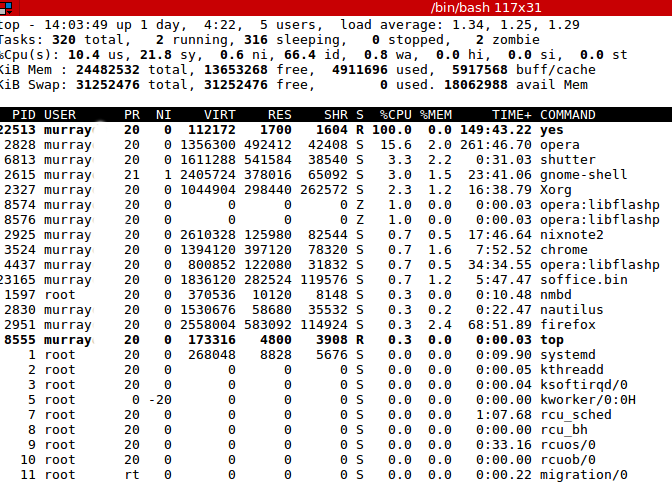
\includegraphics[scale=0.5]{figures/top_white}\\

\subsubsection{top's interactive commands}

\begin{tabularx}{\linewidth}{>{\bfseries}X | X} % the X is needed to wrap text
\caption{top's interactive commands}\label{table:top-controls}\\ % title of Table
\toprule
\normalfont{Command} & Action \\% inserts table heading, unbolds 1st column heading
\midrule
h & display help for interactive commands\\[2mm]	
d or s & set update interval \\[2mm]
x & highlight current sort field, display metrics in bold\\[2mm]
u & change effective user to monitor or all users\\[2mm]
l or t or m & toggles to hide/display\emph{ top's} top line (load), next two lines (tasks and \% cpu), last two lines (memory and swap info)\\[2mm]	
k & kill a task by PID\\[2mm]
r & renice a task by PID\\[2mm]	
f and s and enter & set sort field\\[2mm]
f and space & toggles display\\[2mm]
f and right-arrow to select and up/down arrow to move & moving field column\\[2mm]
q & quit top window and return to command prompt\\[2mm]
\bottomrule
\end{tabularx}

\subsubsection{top at the command line}

We can start a \keyword{top} session from the command line passing various parameters and settings to the \emph{top}.

\begin{table}[!h]
\caption{Using \emph{top} at the command line}
\begin{tabular}{|>{\bfseries}l p{12cm}|}
\hline
\normalfont{Command} & Action \\\hline
top -n1 -b | head -10 & Run only one iteration of the \keyword{top} command. This prints 10 lines which results in only the top 3 processes listed due to 5 lines for the Summary Area, a blank line, the table heading, and then the task area. So, only 3 lines left for the process list. If you use this method, add \# of processes you want to 7 for the \emph{head} option. This issue is addressed in the next command.\\[3mm]
top -b -d5 -n10 -u mgc & Run 10 iterations of \emph{top} with a 5 second delay for processes belonging to user \emph{mgc}. All processes are listed for \emph{mgc}, 10 distinct \emph{top} tables are generated. Each table displays the 5 lines of the Summary Area as well as all processes for user mgc.\\[3mm]
\multicolumn{2}{|l|}{\textbf{top -n1 | egrep -v "top|Tasks|Cpu|Mem|Swap"}}\\
& Run 1 iteration of the \emph{top} command, but remove the top 5 lines of the Summary Area, that is, the lines beginning with these keywords.\\[3mm]	
\multicolumn{2}{|l|}{\textbf{top | egrep -v "top|Tasks|Cpu|Mem|Swap|PID" | tee -a top.log}}\\
& Run and display the \emph{top} command until you manually end the command...and \emph{tee} the output to the file \textsl{top.log}, remove the top five lines of the Summary Area and the table headings for the task area.\\[3mm]
\hline
\end{tabular}
\end{table}

\subsection{hop over to htop}

\textit{I recommend that you install the \keyword{htop} package}. This package is a more user-friendly version of \emph{top}. I will not display more than the initial \emph{htop} screen that appears after you type the \emph{htop} command. Like, \emph{top}, the \emph{htop} window is created using \emph{ncurses.} For more information, please see this \href{https://en.wikipedia.org/wiki/Ncurses}{ncurses} URL. \emph{htop} has a menu driven system at the bottom of the screen. However, some of the function keys will be captured by your operating system and even by your terminal window. It is best just to click the menus using your mouse. 

\begin{description}
	\item[htop's advantages over top]
\end{description}
\begin{itemize}
	\item \tbi{more intuitive:} You can quickly grasp how to interact with \emph{htop} whereas you would have to use \emph{top's} help menu.
	\item \tbi{enhanced interactive commands:} Interactive commands are more numerous and powerful.
	\item \tbi{scroll vertically and horizontally:} With \emph{top} information can be clipped. With \emph{htop}, you can scroll horizontally to reveal all the information.
	\item \tbi{mouse driven:} You can use the mouse to select items and then use the menu system or interactive commands.
	\item \tbi{tree view available:} You can see a processes hierarchy, that is, see the parent-child relationship.
	\item \tbi{killing and renicing:} These tasks can be done without entering PIDs. Instead use the mouse  to select and then the menus to select the operation.
\end{itemize}

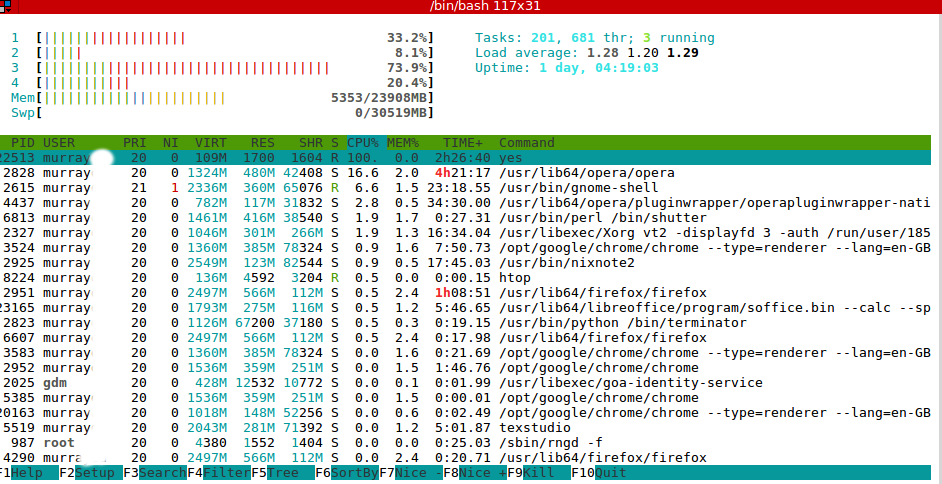
\includegraphics[scale=0.5]{figures/htop_white}\\

However, there is one area where \keyword{top} excels and exceeds the capability of \keyword{htop} and that is at the command line. Take a look at the number of options available to each command in the following section. I am using my \emph{.bashrc m-} function to show the options available to start each command.

Note, when \emph{top} is run in \emph{batch mode}, you cannot interact with \emph{top} as you can when \emph{top} is run in \emph{table mode}. That is, you cannot interrupt \emph{top} to issue the interactive commands.

\begin{lstlisting}[escapeinside={¿}{¿},frame=single,breaklines,columns=fixed]
¿\tld¿ m- htop
-d --delay=DELAY
-C --no-color --no-colour
-h --help
-p --pid=PID,PID...
-s --sort-key COLUMN
-u --user=USERNAME
-v --version

¿\tld¿ m- top
-h | -v	:Help/Version
-b  :Batch-mode operation 
-c  :Command-line/Program-name toggle
-d  :Delay-time interval as:  -d ss.t (secs.tenths)
-H  :Threads-mode operation
-i  :Idle-process toggle
-n  :Number-of-iterations limit as:  -n number
-o  :Override-sort-field as:  -o fieldname
-O  :Output-field-names
-p  :Monitor-PIDs mode as:  -pN1 -pN2 ...  or  -pN1,N2,N3 ...
-s  :Secure-mode operation
-S  :Cumulative-time toggle
-u | -U	:User-filter-mode as:  -u | -U number or name
-w  :Output-width-override as:  -w [ number ]
\end{lstlisting}

\subsection{over the top to atop}

Another interesting tool that can be used alongside \keyword{top} and \keyword{htop} is \keyword{atop}. One advantage that this package has is that it gives a historical summary of system and process activity since the last boot. For help with interactive commands, just type \emph{h}. The \emph{atop} table is split in two. The top of the table shows information on processes, cpu and memory usage, disk usage, and network usage. The bottom of the table shows the historical system and process activity since the last boot.

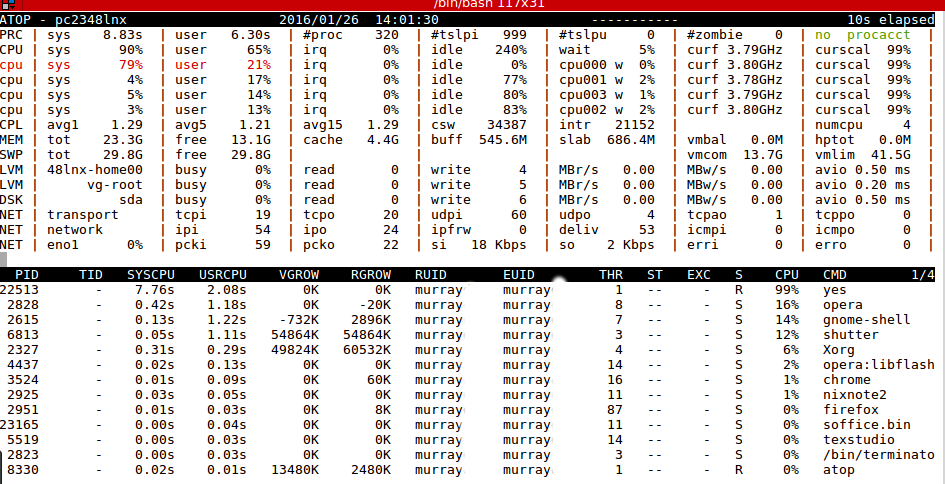
\includegraphics[scale=0.5]{figures/atop_white}

\textit{My suggestion is to use all three tools according to your needs.} 

\begin{description}
	\item[Summary of process monitoring tools as per manpages]
\end{description}
\begin{itemize}
	\item \tbi{top:} display Linux processes
	\item \tbi{htop:} interactive process viewer
	\item \tbi{atop:} Advanced System \& Process Monitor	
\end{itemize}

\section{killing processes}

\subsection{killall}

The following table lists some of the ways of killing or ending processes. \textit{Tread carefully...you are issuing these commands as \emph{sudo}}.

\begin{tabularx}{\linewidth}{>{\bfseries}X | X} % the X is needed to wrap text
\caption{killall}\label{table:killall}\\ % title of Table
\toprule
\normalfont{Command} & Action \\% inserts table heading, unbolds 1st column heading
\midrule
pgrep yes & list the process ids for all instances of the \emph{yes} command\\[2mm]
pgrep -u username yes & list process ids for \emph{yes} command for user \emph{username}\\[2mm]
killall yes & kill instances of \emph{yes} command...owned by you\\[2mm]
sudo killall yes & kill all instances of \emph{yes} command for all users...only root and sudoers can do this\\[2mm]
\bottomrule
\end{tabularx}

\begin{lstlisting}[escapeinside={¿}{¿},frame=single,breaklines,columns=fixed]
¿\tld¿ pgrep yes
6704
12307

¿\tld¿ pgrep -u mgc yes
12307

¿\tld¿ pgrep -u mgcr yes
6704
#
# I knew that both mgc and mgcr users had an instance of yes running. But suppose, you had a system with hundreds of users logged on. How would you get the yes PID for all users?
#
¿\tld¿ for users in `ps aux | awk '{ print $1 }' | sed '1 d' | sort | uniq`;do pgrep -u $users yes;done
12307
6704

¿\tld¿ killall yes
yes(12307): Operation not permitted
[1]+  Terminated              yes > /dev/null
#
# Note, the above command killed the mgcr instance of yes, but not the mgc instance. I issued the command as a non-root user mgcr. Only root and a user with sudo privileges such as the user mgcr can kill all instances.
#
¿\tld¿ sudo killall yes
#
# Has the mgc instance of yes been killed? Oh, yeah!
#
¿\tld¿ pgrep -u mgc yes
¿\tld¿ 
\end{lstlisting}

\subsection{finding all users running a process...a gotcha}\label{subsec:gotcha}

In the above section, I used a very interesting \emph{for} loop to get a list of all users running a process on my system. In order to find out who was logged on, I started by using the commands that are typically used to find who is logged on: \keyword{who}, \keyword{users}, and \keyword{finger}. However, these commands did not reveal all users. None of these commands revealed the user that had a current shell running off a bash shell. This is a \textbf{\color{red}serious} short coming of these commands! \\

\textbf{\color{red}Conclusion:} The commands \emph{who}, \emph{users}, and \emph{finger} do not list users that have bash shell sessions running at a different shell level!

\begin{lstlisting}[escapeinside={¿}{¿},frame=single,breaklines,columns=fixed]
#
# who -u or just who
#
¿\tld¿ who -u
mgcr tty2         2016-01-25 09:43  old         2321 (:0)
mgcr pts/0        2016-01-25 09:44 00:19        2823 (:0)
mgcr pts/1        2016-01-25 09:44   .          2823 (:0)
mgcr pts/2        2016-01-25 09:44 01:14        2823 (:0)
mgcr pts/3        2016-01-25 09:44 00:18        2823 (:0)
#
# Let's try the finger command...
#
¿\tld¿ finger
Login Name             Tty      Idle  Login Time   Office Office Phone Host
mgcr  Murray Davis   tty2       1d  Jan 25 09:43                     (:0)
mgcr  Murray Davis   pts/0      19  Jan 25 09:44                     (:0)
mgcr  Murray Davis   pts/1          Jan 25 09:44                     (:0)
mgcr  Murray Davis   pts/2    1:14  Jan 25 09:44                     (:0)
mgcr  Murray Davis   pts/3      18  Jan 25 09:44                     (:0)
#
# Let's try the users command...
#
¿\tld¿ users
mgcr mgcr mgcr mgcr mgcr
#
# But, just a second, I have another terminal window open for user mgcr and from this terminal I issued the 'su - mgc' command to switch to a bash session for this user. I then started the yes command from that bash window.
#
# From mgc's bash window, I issue these commands...
#
[mgc@LIB2015 ~]$ who -Hm
NAME     LINE         TIME             COMMENT
mgcr pts/3        2016-01-25 09:44 (:0)

[mgd@LIB2015 ~]$ echo $SHLVL
1
#
# Similarily, what's my shell level and psuedo terminal number for my mgcr terminal window?
#
¿\tld¿ who -Hm
NAME     LINE         TIME             COMMENT
mgcr pts/1        2016-01-25 09:44 (:0)

¿\tld¿ echo $SHLVL
2
#
# mgcr is running at shell level 2 and mgc is running at shell level 1
#
# Ok, let's get a unique list of all users running processes on my system using the ps command piped to other commands.
#
# | awk '{ print $1 }' - this first pipe gets only the first field of our output, the username
# | sed '1 d' - this second pipe says delete the first line of output, the heading, USER
# | sort  -  this third pipe says list the usernames in alphabetically order
# | uniq - the last pipe says, only show unique names
#
¿\tld¿ ps aux | awk '{ print $1 }' | sed '1 d' | sort | uniq
avahi
chrony
colord
dbus
gdm
mgc
mgcr
nobody
polkitd
root
rtkit
#
# Ok, assuming, yes is running for the mgc and mgcr users, let's filter the process list on yes.
#
¿\tld¿ ps aux | grep yes | awk '{ print $1 }' | sed '1 d' | sort | uniq
mgc
mgcr
#
# Now, let's use the who command. Notice that the who command  misses the mgc user who is logged into a bash shell window at a different shell level than mgcr.
#
¿\tld¿ who
mgcr tty2         2016-01-25 09:43 (:0)
mgcr pts/0        2016-01-25 09:44 (:0)
mgcr pts/1        2016-01-25 09:44 (:0)
mgcr pts/2        2016-01-25 09:44 (:0)
mgcr pts/3        2016-01-25 09:44 (:0)
\end{lstlisting}

\subsection{pkill and kill -9}

Ok, the following section shows how to kill user processes.


\begin{lstlisting}[escapeinside={¿}{¿},frame=single,breaklines,columns=fixed]
#
# We are logged on as 'mgcr'
#
¿\tld¿ whoami
mgcr
#
# First, let's get a list of all processes being run by user mgc, note that one of the processes is the actual bash window.
#
¿\tld¿ pgrep -l -u mgc
17628 bash
22962 yes
25761 sleep
#
# Alright, let's kill his sleep process.
#
¿\tld¿ pkill -u mgc sleep
pkill: killing pid 25761 failed: Operation not permitted
# 
# Oops, we have to be sudo, so let's use the abreviation for the previous command instead of retyping the command.
#
¿\tld¿ sudo !!
sudo pkill -u mgc sleep

¿\tld¿ pgrep -l -u mgc
17628 bash
22962 yes
#
# Ok, let's use a different method of killing another user's process.
# We are going to use command substitution indicated by the grave accents.
# We could have also used $(pgrep -u mgc yes).
#
¿\tld¿ sudo kill -9 `pgrep -u mgc yes`

¿\tld¿ pgrep -l -u mgc
17628 bash
#
# Alright, so mgc just has his bash session open, he has no other processes running.
#
# Meanwhile, back at mgc's command prompt, he issues the command 'who -Hm'. The output shows that mgcr is logged on. As well, we can see that the yes process was killed and the sleep process terminated. It is possible that it was mgcr who killed mgc's processes!
#
[mgc@LIB2015 ~]$ who -Hm
NAME LINE         TIME             COMMENT
mgcr pts/3        2016-01-25 09:44 (:0)
[1]-  Killed                  yes > /dev/null
[2]+  Terminated              sleep 1000

[mgc@LIB2015 ~]$ echo $SHLVL
1
#
# Let's switch back to the mgcr terminal and check what processes mgc is running. Notice that -bash appears beneath the CMD field, the - indicates that this process is a login shell.
#
¿\tld¿ ps -fu mgc
UID        PID  PPID  C STIME TTY          TIME CMD
mgc       6545  6528  0 13:45 pts/3    00:00:00 -bash
#
# Ok, let's kill the bash session belonging to mgc...which logs him off.
#
¿\tld¿ sudo pkill -u mgc bash
#
# Here is what we see at the mgc bash window.
#
[mgc@LIB2015 ~]$ logout
¿\tld¿ 
#
# Let's log back on as mgc and to see if we can find out who logged us off.
#
¿\tld¿ su -mgc

[mgc@LIB2015 ~]$ who -Hm
NAME  LINE        TIME             COMMENT
mgcr pts/3        2016-01-25 09:44 (:0)
#
# So, the answer is possibly...We can speculate because mgcr is the only user who is logged and who may have logged out mgc.
#
\end{lstlisting}

\subsection{ps and pgrep - more examples}

\begin{lstlisting}[escapeinside={¿}{¿},frame=single,breaklines,columns=fixed]
#
# List all bash sessions.
#
¿\tld¿ pgrep -d, -x bash
9619,9622,9629,9638
#
# Let's try different delimiters between the PIDs.
#
¿\tld¿ pgrep -d\; -x bash
9619;9622;9629;9638

¿\tld¿ pgrep -d\| -x bash
9619|9622|9629|9638
#
# Let's get detailed information on each bash session.
#
¿\tld¿ ps -fp `pgrep -x bash`
UID    PID  PPID  C STIME TTY      STAT   TIME CMD
mgcr  9619  9610  0 14:11 pts/0    SNs+   0:00 /bin/bash
mgcr  9622  9610  0 14:11 pts/1    SNs    0:00 /bin/bash
mgcr  9629  9610  0 14:11 pts/2    SNs+   0:00 /bin/bash
mgcr  9638  9610  0 14:11 pts/3    SNs+   0:00 /bin/bash
#
# Hey, that's interesting. I wonder what would happen if on psuedo terminal 3 (pts/3) we instead issued the command: 'su - mgc' and then repeated our command.
#
¿\tld¿ ps -fp `pgrep -x bash`
UID    PID  PPID  C STIME TTY      STAT   TIME CMD
mgcr  9619  9610  0 14:11 pts/0    SNs+   0:00 /bin/bash
mgcr  9622  9610  0 14:11 pts/1    SNs    0:00 /bin/bash
mgcr  9629  9610  0 14:11 pts/2    SNs+   0:00 /bin/bash
mgcr  9638  9610  0 14:11 pts/3    SNs    0:00 /bin/bash
mgc  11274 11260  0 14:23 pts/3    SN+    0:00 -bash
#
# Under the CMD column, for pts/3, two different pieces of information are shown. The original bash session for mgcr with PID 9638, the parent. The bash login session for mgc is listed next, the child.
#
# Light-bulb: At this point, a light bulb went on and I realised that there was another way to find all users that are logged on. Stay tuned for the explanation...or, click to go there ¿\hyperref[subsec:finduserprocs]{now}¿.
#
# Can we list the proces IDs for multiple users?
#
¿\tld¿ pgrep -u chrony,dbus
951
1008
#
# Let's try to get a little more infomration. It looks like PID 1008 belongs to chrony.
#
¿\tld¿ pgrep -lu chrony,dbus
951 dbus-daemon
1008 chronyd
#
# Ok, but let's be certain as to who owns the processes?
#
¿\tld¿ ps -fp `pgrep -u chrony,dbus`
UID        PID  PPID  C STIME TTY      STAT   TIME CMD
dbus       951     1  0 Jan25 ?        Ssl    0:02 /usr/bin/dbus-daemon --system --address=systemd: --nofork --nopidf
chrony    1008     1  0 Jan25 ?        S      0:00 /usr/sbin/chronyd
#
# Task: Find all processes for all users except: nobody.  We first need to get a list of all users present on the system.
#
¿\tld¿ ps aux | awk '{print $1}' | sed '1 d' | sort | uniq
avahi
chrony
colord
dbus
gdm
lp
mgc
mgcr
nobody
polkitd
root
rtkit

# Ok, let's use pgrep's inverse or -v option.
# Note, this is not a practical way of listing the processes for nobody. I am just using this example to illustrate one use of the inverse switch. You would instead issue this command: 'pgrep -lu nobody'.
#
¿\tld¿ pgrep -lvu avahi,chrony,colord,dbus,gdm,lp,mgd,mgcr,polkitd,root,rtkit
1862 dnsmasq
#
# Let's get the details...note, we have to remove the -l switch.
#
¿\tld¿ ps -fp `pgrep -vu avahi,chrony,colord,dbus,gdm,lp,mgd,mgcr,polkitd,root,rtkit`
UID        PID  PPID  C STIME TTY          TIME CMD
nobody    1862     1  0 Jan25 ?        00:00:00 /sbin/dnsmasq --conf-file=/var/lib/libvirt/dnsmasq/default.conf --lea

\end{lstlisting}

\subsubsection{finding all users running a process...revisited}\label{subsec:finduserprocs}

In the previous section, \hyperref[subsec:gotcha]{finding all users running a process...a gotcha}, I said that the light bulb went on. Here continues my adventure...

\begin{lstlisting}[escapeinside={¿}{¿},frame=single,breaklines,columns=fixed]
#
# The light-bulb went on while I was working on the previous section.
# We can use the following command to find users who are logged onto a 'bash login session' and as well 'bash terminal sessions'. Let's first find all 'bash sessions'.
#
¿\tld¿ ps -fp `pgrep -x bash`
UID    PID  PPID  C STIME TTY      STAT   TIME CMD
mgcr  9619  9610  0 14:11 pts/0    SNs    0:00 /bin/bash
mgcr  9622  9610  0 14:11 pts/1    SNs    0:00 /bin/bash
mgcr  9629  9610  0 14:11 pts/2    SNs+   0:00 /bin/bash
mgcr  9638  9610  0 14:11 pts/3    SNs    0:00 /bin/bash
mgc      11274 11260  0 14:23 pts/3    SN+    0:00 -bash
#
# Ugh, that's unwieldly! But, we know that if we want just 'bash login sessions', we just have to look for -bash under the CMD column.
#
# Here is the only way that I could get just that line, using command substitution.
#
¿\tld¿ ps -fp `pgrep -x bash` | awk '$9 == "-bash" {print}'
mgc      11274 11260  0 14:23 pts/3    SN+    0:00 -bash

# So, mgc is logged onto a 'bash login session' on pts/3. I next logged this user onto pts/0 and changed his shell from bash to sh and logged back out. Note that the command prompt changed from ¿\tld¿ to sh-4.3$ when I changed my shell.
#
¿\tld¿ su - mgc
Password: 

¿\tld¿$ chsh -s /bin/sh
Changing shell for mgc.
Password: 
Shell changed.
sh-4.3$ exit
#
# Note, I had to logout and back on to the pts/0 before I could list all 'sh login sessions' from another terminal window. On pts/0, I issue these commands.
#
¿\tld¿$ su - mgc
Password: 

sh-4.3$ echo $SHELL
/bin/sh
sh-4.3$ 
#
# Now, from my mgcr terminal window, I enter this command to get all sh shells. Note, there is no STAT column, there are only 8 columns, whereas when listing bash shells there were 9 columns. On pts/2, I issue these commands. If there are no current sh sessions, you will get an error if you issue the following command.  So, you would want to send errors to /dev/null.
#
¿\tld¿ ps -fp `pgrep -x sh`
UID        PID  PPID  C STIME TTY          TIME CMD
mgc     16780 16768  0 15:06 pts/0    00:00:00 -sh
#
# Since there are only 8 columns, we would have to awk on the 8th field .
#
¿\tld¿ ps -fp `pgrep -x sh` | awk '$8 == "-sh" {print}'
mgc      16780 16768  0 15:06 pts/0    00:00:00 -sh
#
# We would only have to use the longer command with the pipe to awk, if the default shell on the system was sh. We would only want the 'sh login sessions' indicated by -sh and not the regular 'sh terminal sessions' indicated by /bin/sh.
#
# Remember, if you wanted to be absolutely sure that you found all users regarless of the shell that they were using, you would have to look for all types of shells...which can be found with the chsh command. 
#
¿\tld¿ chsh --list-shells
/bin/sh
/bin/bash
/sbin/nologin
/usr/bin/sh
/usr/bin/bash
/usr/sbin/nologin
/usr/bin/tmux
/bin/tmux
/usr/bin/zsh
/bin/zsh
#
# You could create a command similar to the 'ps -fp' command for each type of shell. However, we need to address the error when there are no current sessions for the selected shell. I only show a part of the actual error message. When I issued this command, I had no current 'sh login sessions' open.
#
¿\tld¿ ps -fp `pgrep -x sh` | awk '$9 == "-sh" {print}'
error: list of process IDs must follow -p
#
# So, let's send the error message to the black hole. Note where I put the '2 > /dev/null' which is used to send stderr to the black hole. If you put this code section at the end of the command you would still get the error message.
# 
¿\tld¿ ps -fp `pgrep -x sh` 2 > /dev/null | awk '$9 == "-sh" {print}'
¿\tld¿
\end{lstlisting}

\subsection{sending commands to another terminal window}

This may appear as somewhat trivial, but suppose you wanted to send a command to another terminal window using its pseudo terminal number.

\begin{lstlisting}[escapeinside={¿}{¿},frame=single,breaklines,columns=fixed]
#
# How many terminal windows do I have open? I can simply list the files in the /dev/pts folder. ptmx is the psuedoterminal master/slave. I will not cover this concept. Below, we see that I have 4 pseudo terminal sessions open that are numbered 0 to 3.
#
# What is my pseudo terminal number?
#
¿\tld¿ who -Hm
NAME     LINE         TIME             COMMENT
mgcr pts/1        2016-01-27 14:38 (:0)
#
# We can also simply type...
#
¿\tld¿ tty
/dev/pts/1
#
# And, it is this full path format that I will use to send my commands to another terminal session. But, first, what are the pseudo terminal numbers that are currently open?
#
¿\tld¿ ls /dev/pts
0  1  2  3  ptmx
#
# From pts/1, I want to send the ls command to pts/3. That is, I want to send the file/directory list of my current directory to pts/3. I would do this by redirecting the ls command to pseudo terminal 3's full dev path.
#
¿\tld¿ ls > /dev/pts/3
#
# To indicate that I am at pts/3, I issue the tty command.
#
¿\tld¿ tty
/dev/pts/3
#
# And, after I issue the ls command on pts/1, the following file list starts to appear at the blank pts/3 command prompt. I elided most of the output since the file list is quite long.
#
¿\tld¿ anaconda    login.keyring.bu   rpmbuild
anaconda.old    ls.man             Runtastic
.
.
LaTeX           Public             zdesktop
latextut.rar    roder.sh
#
# However, there is a problem. I have to hit the enter key at pts/3 to return to its command prompt.
#
\end{lstlisting}

Click \href{http://www.humbug.in/2010/utility-to-send-commands-or-data-to-other-terminals-ttypts/}{Pritak Sinha} who has developed a C script called \tbi{ttyecho}. I will not display the code, but here is how you would send the \emph{ls} command from pts/1 to pts/3.

\begin{lstlisting}[escapeinside={¿}{¿},frame=single,breaklines,columns=fixed]
sudo ttyechno -n /dev/pts/3 ls	
\end{lstlisting}

The above command would send the output of the current directory of the source pseudo terminal to the destination pseudo terminal along with a carriage return. The script works flawlessly! Note, you must precede the command with \emph{sudo}. Where would you place this script? Does \emph{sudo} know about its path? Refer to chapter 2 and the discussion of \hyperref[sec:sudo]{sudo's PATH setting}.

\subsection{Let's be nice and all just get along!}

\subsubsection{Introduction}

All processes run with an assigned priority level. You can change this priority level using two commands: \keyword{nice} and \keyword{renice}. The Linux Kernel manages all processes in order to allocate CPU time according to a complex algorithm that establishes priority. Thankfully, this priority level can be changed when we want to assign more or less CPU resources to a process.\\

The process priority ranges from -20 to +19, the metric is called the \emph{nice} value. Think inversely when it comes to the metric, -20 represents the highest priority and +19 represents the lowest priority. Also, \emph{nice} values are only integer values.

\subsubsection{finding out how nice we really are}

\begin{lstlisting}[escapeinside={¿}{¿},frame=single,breaklines,columns=fixed]
#
# Ok, let's start our trusty sleep command.
#
¿\tld¿ sleep 1000 &
[1] 15587
#
# How can we see sleep's nice value. Let's try a couple of commands that we have already used.
#
¿\tld¿ ps -fp `pgrep -x sleep`
UID    PID  PPID  C STIME TTY      TIME     CMD
mgcr 15587 24107  0 08:47 pts/1    00:00:00 sleep 1000
#
# Hmm, no nice column. Remember, pgrep -x sleep, provides the PID of sleep, so we could just issue this command.
#
¿\tld¿ ps -fp 15587
UID    PID  PPID  C STIME TTY      TIME     CMD
mgcr 15587 24107  0 08:47 pts/1    00:00:00 sleep 1000
#
# Alright, how about grepping sleep from our 'ps aux' output.
#
¿\tld¿ ps aux | grep sleep
mgcr 15587  0.0  0.0 112176   712 pts/1    S    08:47   0:00 sleep 1000
mgcr 17661  0.0  0.0 116996  2240 pts/1    S+   09:02   0:00 grep --color=auto sleep
#
# Two things annoying about this output. We see the pipe to, grep sleep, process listed and there are no headings.
#
¿\tld¿ ps aux | head -1 ; ps aux | grep sleep | grep -v grep
USER   PID %CPU %MEM    VSZ   RSS TTY      STAT START   TIME COMMAND
mgcr 17238  0.0  0.0 112176   796 pts/1    S    08:58   0:00 sleep 1000
#
# Well, that got rid of 'grep sleep'. We can also use && instead of the semi-colon.
#
¿\tld¿ ps aux | head -1 && ps aux | grep sleep | grep -v grep
USER   PID %CPU %MEM    VSZ   RSS TTY      STAT START   TIME COMMAND
mgcr 17238  0.0  0.0 112176   796 pts/1    S    08:58   0:00 sleep 1000
#
# But, gosh darn, we still don't see the nice value.
#
¿\tld¿ ps -eo %U%p%n | grep sleep
¿\tld¿ 
#
# Hey, nothing was returned. Why?
#
¿\tld¿ ps -eo %U%p%n%c | grep sleep
mgcr 15587   0 sleep
#
# Oh yeah, if I am grepping sleep which is the command, I have to include the command column (%c). So, I see that 0 is the nice value, but I want the heading.
#
¿\tld¿ ps -eo %U%p%n%c | head -1 && ps -eo %U%p%n%c | grep sleep
USER   PID  NI COMMAND
mgcr 15587   0 sleep
#
# Another way to see the nice value...
#
¿\tld¿ ps -al | head -1 && ps -al | grep sleep
F S   UID   PID  PPID  C PRI  NI ADDR SZ WCHAN  TTY          TIME CMD
0 S 1858215107 15587 24107  0 80 0 - 28044 hrtime pts/1  00:00:00 sleep
#
# Hmm, that did not line up... we can see that the 8th field is the nice value, which equals 0. Because of alignment issues it looks like the nice value is 80.  Let's first just get just the 8th column.
#
¿\tld¿ ps -al | head -1 | tr -s ' ' | cut -d ' ' -f 8 && ps -al | grep sleep | tr -s ' ' | cut -d ' ' -f 8
NI
0
#
# Yeah, and I am going to remember that command!
# tr -s ' ' convert any contiguous spaces to  a single space
# cut -d ' ' -f 8 use a space as a delimiter and get the 8th field
# the first command up to the && gets the heading
# the command after the && gets the actual 'nice' value for 'sleep'.
#
# There has to be an easier way! Also, I had to start a new sleep session since my previous one ended, hence the new PID.
#
¿\tld¿ ps -fl -C yes
F S UID    PID  PPID  C PRI  NI ADDR SZ WCHAN  STIME TTY          TIME CMD
0 R mgcr 19912 24107 99  93   0 - 28043 -      10:24 pts/1    00:18:28 yes
#
# And, we can also use this command...remember spaces in the list of field options leads to an error!
#
¿\tld¿ ps -o pid,user,nice -C sleep
PID   USER   NI
19912 mgcr   0
#
# Hey, how many seconds did I say to sleep?
#
¿\tld¿ ps h -o pid,user,nice,command -C sleep
PID   USER   NI COMMAND
19912 mgcr   0  sleep 10000
#
# I don't want the heading...I may be working on writing a script. This is counter intuitive, h means 'no heading'.
#
¿\tld¿ ps h -o pid,user,nice,command -C sleep
19912 mgcr   0 sleep 10000
#
# Ok, let's just get the nice value of sleep.
#
¿\tld¿ ps  h -o nice -C sleep
0
#
# Suppose we just know the PID of the command, not the command itself.
#
¿\tld¿ ps  h -o nice -p 19912
0
\end{lstlisting}

\subsubsection{nice to see you}
It turns out the the Kernel gives each new process a \emph{nice} value of 0. That is not the lowest \emph{nice} value, it is a mid-road value. Remember, \emph{nice} values range from -20 to +19.\\

\begin{itemize}
\item \tbi{\keyword{nice}} - use this command to set the \emph{nice} value for new commands
\item \tbi{\keyword{renice}} - use this command to modify the \emph{nice} value of existing commands
\item \tbi{\keyword{denice}} - \href{https://www.youtube.com/watch?v=JKYF_h2K7oU}{a  Key and Peel sketch on Youtube}
\end{itemize}

\begin{lstlisting}[escapeinside={¿}{¿},frame=single,breaklines,columns=fixed]
#
# We begin by killing our previous sleep session
#
¿\tld¿ killall sleep
[1]+  Terminated              sleep 100000
#
# Let's create a new sleep process with a nice value of 10...low priority, note we used -10, not 10. Confusing?
#
¿\tld¿ nice -10 sleep 1000 &
[1] 24361
#
# Let's just get the nice value of sleep.
#
¿\tld¿ ps  h -o nice -C sleep
10
#
# What if we wanted a nice value of -10 for our sleep command? That is, we wanted to give it a higher 'nice' value. To make it even more confusing, we have to preceed -10 with another minus sign...and we have to do this as root. This likely makes sense to those with a math background.
#
¿\tld¿ killall sleep
[1]+  Terminated              nice -10 sleep 1000
#
# Ok, let's try setting the nice value of sleep below zero.
#
¿\tld¿ nice --10 sleep 1000 &
[1] 26304
nice: cannot set niceness: Permission denied
#
# We could not set the nice value to -10, but the command to start sleep was successful. We just ended up with a sleep process with the default nice value of zero.
#
¿\tld¿ ps  h -o nice -C sleep
0
#
# We must be root to set a negative nice value. As explained above, we specify a negative value by preceding the metric with another negative sign. We see that we now have a second sleep process with a priority of -10 and a PID of 26356.
#
¿\tld¿ sudo nice --10 sleep 1001 &
[2] 26356
¿\tld¿ ps  h -o nice -C sleep
0
-10
#
# Let's 'killall' the sleep processes.
#
¿\tld¿ killall sleep
sleep(26360): Operation not permitted
[1]-  Terminated              nice --10 sleep 1000
#
# Obviously, a non-root user cannot kill a root process, but we did kill our sleep process.
#
¿\tld¿ sudo killall sleep
[2]+  Done                    sudo env PATH=$PATH nice --10 sleep 1001
#
# Hey, cool! 'sudo env PATH=$PATH' precedes our actual command. Remember that we created an 'alias sudo' in our .bashrc file. The reason that it appears now is that I began working on this section after I added that alias to my .bashrc.
#
\end{lstlisting}	

\textbf{Conclusion: }Only \emph{root} can create a process with a \keyword{nice} value below 0, i.e., high priority nice values. Let's now look at \keyword{renice}.\\

\subsubsection{Nice? I want to be nicer?}

\begin{lstlisting}[escapeinside={¿}{¿},frame=single,breaklines,columns=fixed]
# 
# Let's begin by killing any sleep session...hmm, sleep slept.
#
¿\tld¿ sudo killall sleep
sleep: no process found
#
# Instead of worrying about under sleeping, let's switch to our yes command.
#
¿\tld¿ yes > /dev/null &
[1] 28091
#
# Let's get a full listing of the yes process by command name.
#
¿\tld¿ ps -fl -C yes
F S UID    PID  PPID  C PRI  NI ADDR SZ WCHAN  STIME TTY          TIME CMD
0 R mgcr 28091  3079 99  80   0 - 28043 -      13:20 pts/0    00:00:13 yes
#
# Let's get a full listing of the yes process using its PID.
#
¿\tld¿ ps -fl -p 28091
F S UID    PID  PPID  C PRI  NI ADDR SZ WCHAN  STIME TTY          TIME CMD
0 R mgcr 28091  3079 99  80   0 - 28043 -      13:20 pts/0    00:00:25 yes
#
# Let's just get the nice value of the yes command.
#
¿\tld¿ ps  h -o nice -C yes
0
#
# Nah, I also want the PID, command, and nice fields.
#
¿\tld¿ ps axo pid,comm,nice  | grep yes
27312 yes               0
#
# Hmm, I don't like all that extra space after yes.
#
¿\tld¿ ps axo pid,comm,nice  | grep yes | tr -s " "
27312 yes 0
#
# We can give yes a lower priority, that is, a positive nice value.
#
¿\tld¿ renice 13 -p 28091
28091 (process ID) old priority 0, new priority 13
#
# Let's confirm.
#
¿\tld¿ ps  h -o nice -C yes
13
#
# But, we cannot give it a higher priority...and with renice we can use a single minus sign.
#
¿\tld¿ renice -13 -p 28091
renice: failed to set priority for 28091 (process ID): Permission denied

¿\tld¿ ps  h -o nice -C yes
13
#
# So, we need sudo.
#
¿\tld¿ sudo renice -13 -p 28091
28091 (process ID) old priority 13, new priority -13

¿\tld¿ ps  h -o nice -C yes
-13
#
# Ok, we had to sudo to give it a higher priority, can we now lower that priority? Obama!
#
¿\tld¿ renice 13 -p 28091
28091 (process ID) old priority -13, new priority 13

¿\tld¿ ps  h -o nice -C yes
13
#
# Ok, but can we increase the priority keeping it above 0? Seems not. We can lower it, but not raise it after we lower it...unless we are sudo.
#
¿\tld¿ renice 5 -p 28091
renice: failed to set priority for 28091 (process ID): Permission denied
#
# Can we reset the priority for all processes for a single user?
#
¿\tld¿ su - mgc
Password:
#
# At this point, we just have our shell process running.
# 
¿\tld¿ ps -u mgc
PID   TTY          TIME CMD
29302 pts/3    00:00:00 sh
29358 pts/3    00:00:00 ps
#
# Let's create two more processes.
#
¿\tld¿ sleep 100000 &
[1] 29382

¿\tld¿ yes > /dev/null &
[2] 29418
#
# What are our nice values?
#
¿\tld¿ ps h -o nice
0
0
0
0
#
# Let's see a bit more information.
#
¿\tld¿ ps h -o user,nice,command
mgc        2 -sh
mgc        2 sleep 100000
mgc        2 yes
mgc        2 ps h -o user,nice,command
#
# We are logged on as mgc. For all of our processes, we can lower the 'nice' value to 2.
#
¿\tld¿ renice 2 -u mgc
1000 (user ID) old priority 0, new priority 2
#
# Even our sh shell has a lower priority.
#
¿\tld¿ps h -o user,nice,command
mgc        2 -sh
mgc        2 sleep 100000
mgc        2 yes
mgc        2 ps h -o user,nice,command	
#
# And, as we learned above, we cannot suddenly try to increase the priority of all processes, for example, try to set all processes to a nice value of 1.
#
¿\tld¿ renice 1 -u mgc
renice: failed to set priority for 1000 (user ID): Permission denied
\end{lstlisting}

\subsubsection{summary}

Note: With some of the \keyword{ps} headings, we can use abbreviations. For example, you can use \emph{comm} for \emph{command}. In the examples below, I am using a \emph{pid} value of 1010, a \emph{nice} value of 12 a \keyword{renice} value of -13, a group name of \emph{mygrp}, and a process called \emph{yes}. Non-root users can increase  the nice value (lower the priority) of one of their processes, but they cannot decrease the nice value (increase the priority) even after they have previously increased the nice value of this process. Non-root users can only set a positive nice value for their processes. The \emph{root} user can set, \emph{nice}, and reset, \emph{renice}, any value of any process for any user.

\begin{tabularx}{\linewidth}{>{\bfseries}X | X} % the X is needed to wrap text
\caption{nice and renice}\label{table:nicely}\\ % title of Table
\toprule
\normalfont{Command} & Action \\% inserts table heading, unbolds 1st column heading
\midrule
ps axo pid,command,nice | less & Get a tabular, formatted-with-heading listing of all processes and pipe to \emph{less} so that you can \emph{spacebar} through the listing.\\[2mm]
ps -fl -C yes & Get a tabular, formatted with heading listing of all processes  named \emph{yes}\\[2mm]
ps -o pid,user,nice,command -C yes & Get a tabular, formatted-with-heading listing of all processes named \emph{yes}, but only show \emph{pid}, \emph{user}, \emph{nice}, and \emph{command} fields.\\[2mm]
ps -o pid,user,nice,command -p 1010 & Get a tabular, formatted-with-heading listing of the process for PID (1010), but only show \emph{pid}, \emph{user}, \emph{nice} value, and \emph{command} fields.\\[2mm]
ps  h -o nice -C yes & Just display the numerical \emph{nice} value of  processes named \emph{yes}.\\[2mm]
ps  h -o nice -p 1010 & Just display the numerical \emph{nice} value for \emph{pid} number 1010.\\[2mm]
nice -12 yes & Non-root and root user, start \emph{yes} with a positive \emph{nice} value of 12. Non-root users can only set \emph{nice} to positive values.\\[2mm]
nice 12 yes & Same as above. With \emph{nice}, the value can be -12, 12, +12. End result, \emph{nice} value of positive 12.\\[2mm]
sudo nice -{}-{}12 yes & To set a negative nice value,-12, use two consecutive negative signs. Only \emph{root} can set a negative \emph{nice} value.\\[2mm]
renice 12 -p 1010 & If teh starting nice value is 0, both non-root and root users, can change the \emph{nice} value from 1 to 20 for \emph{pid} number 1010. Non-root user can only lower his processes \emph{nice} values so the starting \emph{renice} value for a non-root user would be 1. That is, he could change a 0 to a 1. This example, for a non-root user assumes existing \emph{nice} value is between 0 and 11.\\[2mm]
Alternatives & Note, we can also use the optional \emph{-n} = nice number option instead of just supplying the nice number, but this option must always go first.\\[2mm]
renice -n 12 -p 1010 & Same as \emph{renice 12 -p 1010}.\\[2mm]
renice -n +12 -p 1010 & Same as above.\\[2mm]
sudo renice -12 -p 1010 &  Only root can set a negative \emph{nice} value. In the case of \emph{renice}, -12 does equal -12. \\[2mm]
sudo renice -n -13 -g mygrp & Change priority of all processes owned by group \emph{mygrp}.\\[2mm]
sudo renice -13 \tgr{pgrep -u mgcr} & Change priority of all processes owned by user \emph{mgcr}.\\[2mm]
sudo renice -13 -u mgcr & An even easier way to do this.\\[2mm]
\bottomrule
\end{tabularx}

\section{I got a grip on you - \keyword{lsof} and \keyword{fuser}}

Sometimes, when you try to delete a file, you will get a vaguely-worded error message saying that you cannot delete the file because it is locked by some process. So, how do you find that locking process? At times, you may also be curious as to what users are running a specific process.

\begin{tabularx}{\linewidth}{>{\bfseries}X | X} % the X is needed to wrap text
\caption{lsof and fuser}\label{table:processes-lsof}\\ % title of Table
\toprule
\normalfont{Command} & Action \\% inserts table heading, unbolds 1st column heading
\midrule
lsof \$(which sshd) & What users are running the \emph{sshd} process? That is, who is connected to my system using the \emph{ssh} protocol?\\[2mm]
lsof -u root & What processes is the \emph{root} user running?\\[2mm]	
lsof -c sshd & What calls are being made by the \emph{sshd} command?\\[2mm]
fuser -v /home/mgcr & What processes are attached to my home directory. The \emph{-v} option provides a header.\\[2mm]
fuser -km /home/mgcr & Kill all those processes attached to my home directory.\\[2mm]
\bottomrule
\end{tabularx}

\section{Limit the number of user processes}

A multi-user server with shared resources can easily become overloaded. We therefore may want to limit the number of connections any one user can have. Alternatively, on a high-performance server, we may actually want to increase the limits. For RHEL, CentOS, and Fedora systems there are a couple of key places where you can find information on resource limits.

\subsection{Key configuration information and files}

\begin{lstlisting}[escapeinside={¿}{¿},frame=single,breaklines,columns=fixed]
¿\tld¿ cat /proc/1/limits
Limit                     Soft Limit           Hard Limit           Units     
Max cpu time              unlimited            unlimited            seconds   
Max file size             unlimited            unlimited            bytes     
Max data size             unlimited            unlimited            bytes     
Max stack size            8388608              unlimited            bytes     
Max core file size        0                    unlimited            bytes     
Max resident set          unlimited            unlimited            bytes     
Max processes             95550                95550                processes 
Max open files            65536                65536                files     
Max locked memory         65536                65536                bytes     
Max address space         unlimited            unlimited            bytes     
Max file locks            unlimited            unlimited            locks     
Max pending signals       95550                95550                signals   
Max msgqueue size         819200               819200               bytes     
Max nice priority         0                    0                    
Max realtime priority     0                    0                    
Max realtime timeout      unlimited            unlimited            us
#
# Here is another way to get that information. Be careful, pay attention to units of measure. In the table above the 'max locked memory' is in bytes, 65536. But, in the output below, its metric is in kbytes, 64. 65536/1024= 64, there are 1024 kilobytes per byte. -S=soft limits, -H=hard limits. See, the description of soft and hard limits below.
# 
¿\tld¿ ulimit -Sa
core file size          (blocks, -c) 0
data seg size           (kbytes, -d) unlimited
scheduling priority             (-e) 0
file size               (blocks, -f) unlimited
pending signals                 (-i) 95550
max locked memory       (kbytes, -l) 64
max memory size         (kbytes, -m) unlimited
open files                      (-n) 1024
pipe size            (512 bytes, -p) 8
POSIX message queues     (bytes, -q) 819200
real-time priority              (-r) 0
stack size              (kbytes, -s) 8192
cpu time               (seconds, -t) unlimited
max user processes              (-u) 95550
virtual memory          (kbytes, -v) unlimited
file locks                      (-x) unlimited

¿\tld¿ ulimit -Ha
core file size          (blocks, -c) unlimited
data seg size           (kbytes, -d) unlimited
scheduling priority             (-e) 0
file size               (blocks, -f) unlimited
pending signals                 (-i) 95550
max locked memory       (kbytes, -l) 64
max memory size         (kbytes, -m) unlimited
open files                      (-n) 4096
pipe size            (512 bytes, -p) 8
POSIX message queues     (bytes, -q) 819200
real-time priority              (-r) 0
stack size              (kbytes, -s) unlimited
cpu time               (seconds, -t) unlimited
max user processes              (-u) 95550
virtual memory          (kbytes, -v) unlimited
file locks                      (-x) unlimited
#
# Is that true for my general user account? What are my open file limits? It turns out that root also has these limits!
#
¿\tld¿ ulimit -Sn; ulimit -Hn
1024
4096
#
# Can we see the ulimit for another user? We can, if we have sudo privileges.
#
¿\tld¿ sudo su -c "ulimit -Hn" mgc
4096
#
# Note, if you tried to get this information for mgc when logged on as a non-root user, you would be prompted for mgc's password. And, if you foo-bared the password or didn't know it, you would get the error message below.
#
¿\tld¿ su - mgc -c "ulimit -Hn"
Password: 
su: Authentication failure
#
# Note, there is no specific man page for ulimit since it is a bash builtin command. I use my mbib function to get just that man page info. This output will help explain the difference between the soft and hard limits.
#
¿\tld¿ mbib ulimit umask
ulimit [-HSTabcdefilmnpqrstuvx [limit]]
Provides control over the resources available to the shell and to processes started by it, on systems that allow such control.  The -H and -S options specify that the hard or soft limit is set  for the  given  resource.   A hard  limit cannot be increased by a non-root user once it is set; a soft limit may be increased up to the value of the hard limit. If neither -H nor -S is  specified, both the soft and hard limits are set.  The value of limit can be a number in the unit specified for the resource or one of the special values hard, soft, or unlimited, which stand  for the  current hard limit,  the  current soft limit, and no limit, respectively.  If limit is omitted, the current value of the soft limit of the resource is printed, unless the -H option is given.  When  more than  one resource is specified, the  limit  name and unit are printed before the value. Other options are interpreted as follows:
-a     All current limits are reported
-b     The maximum socket buffer size
-c     The maximum size of core files created
-d     The maximum size of a process data segment
-e     The maximum scheduling priority ("nice")
-f     The maximum size of files written by the shell and its children
-i     The maximum number of pending signals
-l     The maximum size that may be locked into memory
-m     The maximum resident set size (many systems do not honor this limit)
-n     The maximum number of open file descriptors (most systems do not allow this value to be set)
-p     The pipe size in 512-byte blocks (this may not be set)
-q     The maximum number of bytes in POSIX message queues
-r     The maximum real-time scheduling priority
-s     The maximum stack size
-t     The maximum amount of cpu time in seconds
-u     The maximum number of processes available to a single user
-v     The maximum amount of virtual memory available to the shell and, on  some systems, to its children
-x     The maximum number of file locks
-T     The maximum number of threads

If  limit is given, and the -a option is not used, limit is the new value of the specified resource. If no option is given, then -f is assumed.  Values are in 1024-byte increments, except for -t, which is  in seconds; -p, which is in units of 512-byte blocks; and -T, -b, -n, and -u, which are unscaled values.  The return status is 0 unless an invalid option or argument is supplied, or an error occurs while setting a new limit.  In POSIX Mode 512-byte blocks are used for the `-c' and `-f' options.
#
# The /etc/security folder contains many folders and files that can be viewed and edited in order to make changes to kernel limits. One key file is limits.conf. Note, by default it contains only comments that help explain its useage.
#
¿\tld¿ ls -la  /etc/security
total 92
drwxr-xr-x.   7 root root  4096 Jan 25 08:45 .
drwxr-xr-x. 167 root root 12288 Feb 15 07:46 ..
-rw-r--r--.   1 root root  4620 Aug 12  2015 access.conf
-rw-r--r--.   1 root root    82 Aug 12  2015 chroot.conf
.
.
-rw-r--r--.   1 root root  3635 Aug 12  2015 group.conf
-rw-r--r--.   1 root root  2422 Aug 12  2015 limits.conf
drwxr-xr-x.   2 root root  4096 Nov 16 13:33 limits.d
.
.
-rw-r--r--.   1 root root   419 Aug 12  2015 sepermit.conf
-rw-r--r--.   1 root root  2179 Aug 12  2015 time.conf

¿\tld¿ cat /etc/security/limits.conf
¿\tbi{\#}¿ /etc/security/limits.conf
¿\tbi{\#}¿
¿\tbi{\#}¿This file sets the resource limits for the users logged in via PAM.
¿\tbi{\#}¿It does not affect resource limits of the system services.
¿\tbi{\#}¿
¿\tbi{\#}¿Also note that configuration files in /etc/security/limits.d directory,
¿\tbi{\#}¿which are read in alphabetical order, override the settings in this
¿\tbi{\#}¿file in case the domain is the same or more specific.
¿\tbi{\#}¿That means for example that setting a limit for wildcard domain here
¿\tbi{\#}¿can be overriden with a wildcard setting in a config file in the
¿\tbi{\#}¿subdirectory, but a user specific setting here can be overriden only
¿\tbi{\#}¿with a user specific setting in the subdirectory.
¿\tbi{\#}¿
¿\tbi{\#}¿Each line describes a limit for a user in the form:
¿\tbi{\#}¿
¿\tbi{\#}¿<domain>        <type>  <item>  <value>
¿\tbi{\#}¿
¿\tbi{\#}¿Where:
¿\tbi{\#}¿<domain> can be:
¿\tbi{\#}¿        - a user name
¿\tbi{\#}¿        - a group name, with @group syntax
¿\tbi{\#}¿        - the wildcard *, for default entry
¿\tbi{\#}¿        - the wildcard %, can be also used with %group syntax,
¿\tbi{\#}¿                 for maxlogin limit
¿\tbi{\#}¿
¿\tbi{\#}¿<type> can have the two values:
¿\tbi{\#}¿        - "soft" for enforcing the soft limits
¿\tbi{\#}¿        - "hard" for enforcing hard limits
¿\tbi{\#}¿
¿\tbi{\#}¿<item> can be one of the following:
¿\tbi{\#}¿        - core - limits the core file size (KB)
¿\tbi{\#}¿        - data - max data size (KB)
¿\tbi{\#}¿        - fsize - maximum filesize (KB)
¿\tbi{\#}¿        - memlock - max locked-in-memory address space (KB)
¿\tbi{\#}¿        - nofile - max number of open file descriptors
¿\tbi{\#}¿        - rss - max resident set size (KB)
¿\tbi{\#}¿        - stack - max stack size (KB)
¿\tbi{\#}¿        - cpu - max CPU time (MIN)
¿\tbi{\#}¿        - nproc - max number of processes
¿\tbi{\#}¿        - as - address space limit (KB)
¿\tbi{\#}¿        - maxlogins - max number of logins for this user
¿\tbi{\#}¿        - maxsyslogins - max number of logins on the system
¿\tbi{\#}¿        - priority - the priority to run user process with
¿\tbi{\#}¿        - locks - max number of file locks the user can hold
¿\tbi{\#}¿        - sigpending - max number of pending signals
¿\tbi{\#}¿        - msgqueue - max memory used by POSIX message queues (bytes)
¿\tbi{\#}¿        - nice - max nice priority allowed to raise to values: [-20, 19]
¿\tbi{\#}¿        - rtprio - max realtime priority
¿\tbi{\#}¿
¿\tbi{\#}¿<domain>      <type>  <item>         <value>
¿\tbi{\#}¿
¿\tbi{\#}¿*               soft    core            0
¿\tbi{\#}¿*               hard    rss             10000
¿\tbi{\#}¿@student        hard    nproc           20
¿\tbi{\#}¿@faculty        soft    nproc           20
¿\tbi{\#}¿@faculty        hard    nproc           50
¿\tbi{\#}¿ftp             hard    nproc           0
¿\tbi{\#}¿@student        -       maxlogins       4
¿\tbi{\#}¿ End of file

\end{lstlisting}

\subsection{Temporary and permanent changes - examples}

Alright, now that we know where to find information on the kernel limits, let's start making some changes. Obviously, since you are messing around with kernel limits, you need to be \emph{root} in order to make the changes. Permanent changes are made by editing \textsl{/etc/security/limits.conf}. Temporary changes are made by using the \keyword{ulimit} command.

\begin{enumerate}
	\item{Bob - Bob is a pain in the ass. He runs an application that opens hundreds of files. Since the file size is unlimited, this tends to use up lots of resources. Let's edit \textsl{/etc/security/limits.conf} and add these lines:\\
		\textbf{bob soft nofile 100}\\
		\textbf{bob hard nofile 100}\\
		Now, instead of the maximum of 1024 files, Bob can only open 100 files.}
	\item{Executives - Members of the executive group watch streaming videos all day. These video files are enormous. Let's limit the file size for the executive group to 1GB or 1000000KB.\\
		\textbf{@executive hard data 1000000}}
	\item{Shackle everyone - Our main server is slowing down to a crawl. Let's temporary limit the number of user processes until we find out what's going on. We issue this command at the command line.\\
		\textbf{sudo ulimit -u 10000}}
\end{enumerate}





\chapter{dnf}
\pagestyle{fancy}
\label{ch:dnf}

\fancyhf{} % here we clear any fancy header settings
%% Note, the first page of every chapter does not have a header.
\fancyhead[EC]{Linux System Administration}
\fancyhead[OC]{\leftmark} % O=odd pages, C= center, leftmark defaults to Chapter number and title
%\fancyhead[EC]{\rightmark} % E = even pages, C = center, rightmark defaults to number of current section
%%
%% Set, headheight to eliminate warning message "Package Fancyhdr Warning: \headheight is too small (12.0pt): Make it at least 13.59999pt.
\setlength{\headheight}{13.99pt} 
%%
% The next line would put a line at the bottom of every page starting from the second page of every chapter, if it was uncommented.
%%
%\renewcommand{\footrulewidth}{1pt}
%%
\cfoot{\thepage} % c = center, foot = footer, thepage = page number
\rhead{
\includegraphics[width=.5cm]{figures/smCanadianFlag}}
		
%%%%%%%%%%%%%%%%%%%%%%%%%%%%%%%%%%%%%%%%%%%%%%%%%%%%%%%%%%%
%%%%%%%%%%%%%%%%%%%%%%%%%%%%%%%%%%%%%%%%%%%%%%%%%%%%%%%%%%%

\section{Introduction}
All RPM-based Linux distributions such as RHEL, CentOS, and Fedora use the \keyword{dnf} package manager. The previous package manager was called \keyword{yum}, which stood for \href{https://en.wikipedia.org/wiki/Yellowdog\_Updater,\_Modified}{\emph{Yellowdog Updater, Modified}}. \emph{dnf} or \emph{dandified yum} is just the next generation of the RPM-based package manager.

The manpage for \emph{dnf} is quite extensive. Likely, you will only use a very limited subset of the available commands. \emph{dnf} is basically used to keep your system up-to-date as well as managing each application: installs, removes, changing versions, etc.

In the table below, I list the commands that I frequently use to manage packages. Some of these commands are available to all non-root users such as the search and info options. You may want to create an alias to simpify things: \emph{alias dnf=\tqs{sudo dnf}}.

\section{Table of dnf commands}

\begin{tabularx}{\linewidth}{>{\bfseries}X | X} % the X is needed to wrap text
\caption{dnf commands}\label{table:dnf-commands}\\ % title of Table
\toprule
\normalfont{Command} & Action \\% inserts table heading, unbolds 1st column heading
\midrule
\textit{\color{red}How to install a package} &\\[2mm]
dnf install pkgname & Install a specific package. You do not have to append the architecture.\\[3mm]
	
\textit{\color{red}How to downgrade a package} & \\[2mm]
dnf downgrade pkgname & Only downgrade this one package, no others.\\[3mm]
	
\textit{\color{red}How to remove a package} & \\[2mm]
dnf remove pkgname & Remove a specific package.\\[2mm]
dnf autoremove &  Remove any legacy packages that are no longer required. These packages may have been installed as pre-requisites for other packages which have been removed from the system.\\[3mm]
	
\textit{\color{red}How to update system \& all packages} & \\[2mm]
dnf update & Update all packages.\\[2mm]
dnf update -x texlive-minted & Update all packages except \emph{texlive-minted}. I had an alias for this command so that the \emph{texlive-minted} package was never updated.\\[2mm]
dnf update pkgname.x86\_64 & Only update this one package, no others, specifying the system architecture.\\[2mm]
dnf update pkgname & Only update this one package, no others. There is no need to append architecture. The kernel figures this out.\\[2mm]
dnf check-updates & Just check and show pending updates, don't start the installation process.\\[3mm]
	
\textit{\color{red}How to search} & \\[2mm]
dnf search pkgname & Search for all packages with the string \emph{pkgname} in the full package name or in the brief description of the package.\\[3mm]
	
\textit{\color{red}How to get info} & \\[2mm]
dnf info pkgname & Get basic information on \emph{pkgname} such as version and release number, summary, and description.\\[3mm]
dnf provides /path/to/command & What package provided this command? Commands that you typically find in \textsl{/usr/bin} and \textsl{/usr/sbin}.\\[3mm]
	
\textit{\color{red}How to list} & \\[2mm]
dnf list installed & Get a list of all packages installed on the system.\\[2mm]
dnf list installed | wc -l & Get a count of the number of packages installed on the system...approximate only.\\[2mm]
dnf list installed | sed \tqs{1,2d} | sed -e \emph{/\textasciicircum{} /d} | wc -l & Remove the count of the first two lines since they are only headers and remove any line beginning with a space. Packages with long names wrap around two lines with the second line begining with a space...accurate.\\[2mm]
dnf list installed | grep pkgname & Is \emph{pkgname} installed?\\[2mm]
dnf list installed pkgname & Is \emph{pkgname} installed? There is no need to use grep. If package is installed, there are three columns of info: package name, version \& release info, and source of package.\\[2mm]
dnf list & Display available (still not installed) and installed packages: three columns: package name c/w architecture, version and release numbers, source of package.\\[2mm]
dnf list | awk \tqs{\{print \$3\}} | sort | uniq & We only want a distinct listing of the sources used to install packages. We can then use the output to grep categories as shown below.\\[2mm]
dnf list available & List all packages that are availble to install...that haven't been installed.\\[2mm]
dnf list available | grep updates & Another way of finding pending updates.\\[2mm]
dnf list available | grep @updates & What packages were installed as part of an update?\\[2mm]
dnf list available | grep pkgname & List both 32-bit and 64-bit packages for \emph{pkgname}.\\[2mm]
dnf list available pkgname & Same as above, \emph{grep} is not needed when referring to specific packages.\\[2mm]
dnf list available | grep pkgname.x86\_64 & Only list the 64-bit package. Or, simply \emph{grep pkgname.x*}.\\[2mm]
dnf list available pkgname.x* & Again, grep is not needed.\\[2mm]
dnf list available | grep pkgname.i686 & Only list the 32-bit package.\\[2mm]
dnf list available pkgname.i* & Same as above.\\[2mm]
dnf list available | grep updates | less & What updates are available? Use the spacebar to scroll through the list.\\[2mm]
dnf list | grep @@commandline & This will list packages installed from the command line...including any dependencies installed with the root package. You must use \emph{grep}.\\[2mm]
dnf list installed | grep *string* & You may not remember the correct package name, but only a part of the package name.\\[2mm]
dnf list installed *string* & Fewer characters to type!\\[3mm]
\bottomrule
\end{tabularx}

\section{Package groups}

According to the \tbi{dnf} manpage, \tbi{groups} are defined as virtual collections of packages. 

\begin{tabularx}{\linewidth}{>{\bfseries}X | X} % the X is needed to wrap text
\caption{dnf groups}\label{table:dnf-groups-commands}\\ % title of Table
\toprule
\normalfont{Command} & Action \\% inserts table heading, unbolds 1st column heading
\midrule
\textit{\color{red}How to manage package groups} & \\[2mm]
dnf group list & List all group packages. Some packages are installed not individually but as part of a collection of packages. The output for this command is separated into three categories: Available environment groups, Installed groups, and Available groups. Alternate forms of this command: dnf grouplist, dnf groups list, but not dnf groupslist.\\[2mm] 
dnf grouplist | grep \tqs{   } | while read line; do dnf groupinfo "\$line"; done & This code was snagged from...\href{http://unix.stackexchange.com/questions/236935/dnf-how-to-find-which-group-package-belongs-to}{List the individual packages contained in each package group}. Note: You are grepping 3 blank spaces.\\[4mm]
dnf grouplist | grep grppkgname | grep \tqs{   } | while read line; do dnf groupinfo "\$line"; done & List the packages that make up the package group  \emph{grppkgname}.\\[6mm]
dnf groupinfo grppkgname & The above command was just listed for illustration, you would not actually use it. You would use this command. \\[2mm]
dnf group remove grppkgname & Remove the \emph{grppkgname} group.\\[6mm]
\bottomrule
\end{tabularx}

\subsection{Listing package groups}

In the code below, when I want a verbose listing of group packages, I use a \emph{grep after} option to deal with a wonky issue that I believe is a \emph{dnf} bug related to non-standard Fedora packages. Without the \emph{grep after} option, I get about 30 lines of what looks like error codes. It is possible that I somehow foobarred my PC and thus the error codes are unique to my PC.

\begin{lstlisting}[escapeinside={¿}{¿},frame=single,breaklines,columns=fixed]
¿\tld¿ dnf group list
Last metadata expiration check performed 0:21:39 ago on Tue Feb  2 07:33:47 2016.
¿\color{red}{Available environment groups:}¿
Minimal Install
Fedora Server
Fedora Workstation
.
.
Web Server
Infrastructure Server
Basic Desktop
¿\color{red}{Available groups:}¿
Administration Tools
Audio Production
Authoring and Publishing
Books and Guides
.
.
Window Managers
#
# There is also a verbose version of this command...that generates some error messages similar to those below that appear right before the 'Available environment groups'.
#
¿\tld¿ dnf grouplist -v
cachedir: /var/tmp/dnf-murrayda-vChWtb
Loaded plugins: download, config-manager, needs-restarting, 
DNF version: 1.1.6
repo: using cache for: fedora
not found deltainfo for: Fedora 23 - x86\_64
not found updateinfo for: Fedora 23 - x86\_64
.
.
google-chrome: using metadata from Thu Feb 11 09:51:16 2016.
Last metadata expiration check performed 0:09:18 ago on Tue Feb 16 09:53:14 2016.
group persistor md version: 0.6.0
¿\color{red}{Available environment groups:}¿
Minimal Install (minimal-environment)
Fedora Server (server-product-environment)
.
.
¿\color{red}{Installed groups:}¿
Editors (editors)
¿\color{red}{Available groups:}¿
Administration Tools (admin-tools)
Audio Production (audio)
.
.
3D Printing (3d-printing)
Window Managers (window-managers)
¿\color{red}{Available language groups:¿|
Oriya Support (oriya-support) [or]
Arabic Support (arabic-support) [ar]
.
.
Vietnamese Support (vietnamese-support) [vi]
Yiddish Support (yiddish-support) [yi]
#
# Ok, let's get rid of the error codes using the 'grep after' option. The output is listed with two names: Formal name (common name).
#
¿\tld¿ dnf grouplist -v | grep -A300 "Available environment groups"
¿\color{red}{Available environment groups:}¿
Minimal Install (minimal-environment)
Fedora Server (server-product-environment)
.
.
Basic Desktop (basic-desktop-environment)
¿\color{red}{Installed groups:}¿
Editors (editors)
¿\color{red}{Available groups:}¿
Administration Tools (admin-tools)
Anaconda tools (anaconda-tools)
Audio Production (audio)
Authoring and Publishing (authoring-and-publishing)
Books and Guides (books)
.
.
XMonad (xmonad)
XMonad for MATE (xmonad-mate)
¿\color{red}{Available language groups:}¿
Oriya Support (oriya-support) [or]
Arabic Support (arabic-support) [ar]
.
.
Vietnamese Support (vietnamese-support) [vi]
Yiddish Support (yiddish-support) [yi]
#
# We can then use the verbose naming convention's common name instead of the formal name in our commands. You need to enclose formal names that have spaces inside double quotes.
#
¿\tld¿ dnf groupinfo "Books and Guides"
Last metadata expiration check performed 0:05:14 ago on Tue Feb 16 09:53:14 2016.

Group: Books and Guides
Description: Books and Guides for Fedora users and developers
Default Packages:
diveintopython
javanotes
ldd-pdf
#
# It is much easier to use the common names provided by the verbose, group list. For example, under Available Groups, we see Books and Guides (books), where books is the common name.
#
¿\tld¿ dnf groupinfo books
Last metadata expiration check performed 0:03:04 ago on Tue Feb 16 09:53:14 2016.

Group: Books and Guides
Description: Books and Guides for Fedora users and developers
Default Packages:
diveintopython
javanotes
ldd-pdf
\end{lstlisting}

\subsection{Installing package groups}

\begin{lstlisting}[escapeinside={¿}{¿},frame=single,breaklines]
#
# Ok, what's inside the Editors group?
#
¿\tld¿ dnf groupinfo editors
Last metadata expiration check performed 0:01:03 ago on Tue Feb 16 08:58:05 2016.

Group: Editors
Description: Sometimes called text editors, these are programs that allow you to create and edit text files. This includes Emacs and Vi.
Optional Packages:
code-editor
cssed
emacs
.
.
vim-enhanced
xemacs
.
.
xmlcopyeditor
zile
¿\tld¿ 
#
# Oh, look, vim-enhanced. When you go to install a group package, you may find that you have previously installed some of its components. Only those components not yet installed get installed. Let's go ahead and install the Editors group. Note, I do not show the output that the install command generates.
#
¿\tld¿ dnf groupinstall editors	
#
# Ok, let's see if we have installed any package groups. Note: sed '$d' deletes last line.
#
¿\tld¿ dnf group list | grep -A50 -i "installed groups" | grep -B50 -i "available groups" | sed '$d'
Installed groups:
Editors
#
# How many packages do we have installed in each group category? Note, the following command does not list the 'Available environment groups'.
#
¿\tld¿ dnf group summary
Last metadata expiration check performed 0:11:28 ago on Tue Feb  2 13:41:23 2016.
Installed Groups: 1
Available Groups: 34
#
# Ok, let's play a little. Let's list our groups again...I elide the full listing for brevity. We see that we do now have a new category called 'Installed Groups'.
#
¿\tld¿ dnf group list
Last metadata expiration check performed 4:58:50 ago on Mon Feb 15 09:49:37 2016.
¿\textit{\color{red}Available environment groups:}¿
Minimal Install
Fedora Server
.
.
Infrastructure Server
Basic Desktop
¿\textit{\color{red}Installed groups:}¿
Editors
¿\textit{\color{red}Available groups:}¿
Administration Tools
Audio Production
.
.
3D Printing
Window Managers
#
# I want a count of the number of packages in each group category. I am going to use the bc command. To understand my command, break it down in its parts. Why do I subtract two in the first two commands? Why don't I need the second 'grep' command in the last command and only subtract 1?
#
¿\tld¿ echo "`dnf group list | grep -A100 "Available environment groups:" | grep -B100 "Installed groups:" | wc -l` -2" | bc
15
¿\tld¿ echo "`dnf group list | grep -A100 "Installed groups:" | grep -B100 "Available groups:" | wc -l` -2" | bc
1
¿\tld¿ echo "`dnf group list | grep -A100 "Available groups:" | wc -l` -1" | bc
34
\end{lstlisting}

Did you know that there are \keyword{hidden package groups}? 

\begin{lstlisting}[escapeinside={¿}{¿},frame=single,breaklines]
#
# As we found out from the above section, when we use the verbose dnf option, we need to remove the error messages from the top of the listing.
#
¿\tld¿ dnf grouplist -v hidden | grep -A300 "Available environment groups"
¿\textit{\color{red}Available environment groups:}¿
Minimal Install (minimal-environment)
Fedora Server (server-product-environment)
.
.
Basic Desktop (basic-desktop-environment)
¿\textit{\color{red}Installed groups:}¿
Editors (editors)
¿\textit{\color{red}Available groups:}¿
Administration Tools (admin-tools)
Anaconda tools (anaconda-tools)
Audio Production (audio)
.
.
XMonad (xmonad)
XMonad for MATE (xmonad-mate)
¿\textit{\color{red}Available environment groups:}¿
Oriya Support (oriya-support) [or]
Arabic Support (arabic-support) [ar]
.
.
Urdu Support (urdu-support) [ur]
Vietnamese Support (vietnamese-support) [vi]
Yiddish Support (yiddish-support) [yi]
#
# Let's compare the number of regular or unhidden packages with the number of hidden packages. We have 50. We subtract 4, 3 four the group headings and 1 for the first line of output of 'dnf grouplist'.
#
¿\tld¿ echo "`dnf grouplist | wc -l` -4" | bc
50
#
# Alright, how many unhidden and hidden group packages do we have? Wow, 198! We still subtract 4. We have no output heading because of the grep, but we now have an additional heading 'Available language groups:'. 
#
¿\tld¿ echo "`dnf grouplist -v hidden | grep -A300 "Available environment groups" | wc -l` -4" | bc
198

¿\tld¿ dnf grouplist -v hidden | grep -A300 "Available environment groups" | grep groups
Available environment groups:
Installed groups:
Available groups:
Available language groups:
#
# Ok, let's get the count of the individual groups. No, change in the number of 'Available environment groups' or 'Installed groups'.
#
¿\tld¿ echo "`dnf group list -v hidden | grep -A100 "Available environment groups:" | grep -B100 "Installed groups:" | wc -l` -2" | bc
15

¿\tld¿ echo "`dnf group list -v hidden | grep -A100 "Installed groups:" | grep -B100 "Available groups:" | wc -l` -2" | bc
1
#
# Note, I have to change the after and before grep metric because the count is above 100.
#
¿\tld¿ echo "`dnf group list -v hidden | grep -A200 "Available groups:" | grep -B200 "Available language groups:" | wc -l` -2" | bc
137
#
# And, finally...
#
¿\tld¿ echo "`dnf group list -v hidden | grep -A200 "Available language groups:" | wc -l` -1" | bc
45
\end{lstlisting}

	\section{\keyword{dnf repositories}}

\emph{dnf} relies on repositories and uses a global configuration file \textsl{/etc/dnf/dnf.conf} and individual \textsl{*.repo} files located in the \textsl{/etc/yum.repos.d} directory. These configuration files tell the system how to find system packages and updates. Although, you can append \emph{repo} configurations settings to the end of the  \textsl{/etc/dnf/dnf.conf} configuration file, this is not recommended. It is must easier to troubleshoot repository issues if you use separate files for each repository.

\begin{lstlisting}[escapeinside={¿}{¿},frame=single,breaklines,columns=fixed]
#
# Here is  a list of my repos files...
#
¿\tld¿ ls /etc/yum.repos.d
adobe-linux-x86_64.repo      hipchat.mydomain.com_clients_linux_yum.repo  rpmfusion-free-updates-testing.repo
_copr_helber-atom.repo       home:garminplugin.repo.old                 rpmfusion-nonfree-rawhide.repo
fedora.repo                  ozonos.repo.old                            rpmfusion-nonfree.repo
fedora-updates.repo          playonlinux.repo                           rpmfusion-nonfree-updates.repo
fedora-updates-testing.repo  rpmfusion-free-rawhide.repo                rpmfusion-nonfree-updates-testing.repo
folkswithhats.repo           rpmfusion-free.repo
google-chrome.repo           rpmfusion-free-updates.repo
#
# An example of a .repo file. Note: I shortened the baseurl for formatting purposes; therefore, this baseurl is incorrect.
#
¿\tld¿ cat _copr_helber-atom.repo 
[helber-atom]
name=Copr repo for atom owned by helber
baseurl=https://copr-be.cloud.fedoraproject.org/results/helber/atom/fedora-release
gpgcheck=1
gpgkey=https://copr-be.cloud.fedoraproject.org/results/helber/atom/pubkey.gpg
enabled=1
enabled_metadata=1
¿\tld¿ 

¿\tld¿ cat /etc/dnf/dnf.conf
[main]
gpgcheck=1
installonly_limit=3
clean_requirements_on_remove=True	
\end{lstlisting}

	\subsection{Disabling a \keyword{repo}}

\begin{enumerate}
	\item{Remove the repo file from \textsl{/etc/yum.repos.d}}
	\item{Rename the repo file's extension, i.e., \textsl{copr\_helber-atom.repo.disabled}}
	\item{Edit the repo file and change the line \emph{enabled=1} to \emph{enabled=0}}
\end{enumerate}

% I had a heck of a time getting the table to stay with the subsection header. I have to revisit this as it is not an optimal solution in terms of typesetting. I also don't like the \newpage command.

\newpage
\subsection{Repo commands}

As with any other \emph{dnf} commands, these commands require \emph{sudo privilege}.

\begin{table}[!htpb]
\caption{repo commands}
\begin{tabular}{|>{\bfseries}l p{6cm}|}
\hline
\normalfont{Command} & Action \\\hline
\textit{\color{red}How to manage repositories} & \\[2mm]
dnf repolist & Three columns of info: repo-id, repo-name and number of packages within repo...not the number of packages installed from this repo.\\[2mm]
dnf repository-packages repo-id list & List the packages from the specified \emph{repo-id}. Output is grouped as \emph{Installed Packages} and \emph{Available Packages}.\\[2mm]
dnf repolist disabled & List of all repos not currently in use.\\[2mm]
dnf repolist enabled & Same as \emph{dnf repolist}.\\[2mm]

\textit{\color{red}1. How to enable repos - by reponame and user/project} & \\[2mm]
dnf copr enable dacr/brackets & \emph{copr} is the repo, \emph{dacr} is the user, and \emph{brackets} is the project. In these three methods of enabling repositories, I am using specific examples.\\[3mm]
dnf copr list helber & Note, to list packages for a specific user \emph{helber} from a specific repos \emph{copr.}\\[3mm]

\textit{\color{red}2. How to enable repos - by repo url} & \\[2mm]
\multicolumn{2}{|l|}{\textbf{\begin{small}dnf config-manager --add-repo=http://negativo17.org/repos/fedora-spotify.repo\end{small}}}\\
& You may have to do a bit of hunting to find the specific link on the repo's website.\\[3mm]	
\multicolumn{2}{|l|}{\textbf{\begin{small}su -c "wget http://rpm.playonlinux.com/ playonlinux.repo -O /etc/yum.repos.d/playonlinux.repo"\end{small}}}\\
& Alternative, download the actual repo file and put it in the repo directory \textsl{/etc/yum.repos.d}. This is how I enabled the \emph{Playonlinux} repo.\\[3mm]

\textit{\color{red}3. How to enable repos - by repo file} & \\[2mm]
Download repo file from repo's website & The repo file is usually on the Overview page of the project. Place the \textsl{project.repo} file in \textsl{/etc/yum.repos.d} directory.\\[3mm]	
\hline
\end{tabular}
\end{table}

\section{Old School}

It used to be a nightmare when you tried to install packages via the old \emph{RPM-Redhat Package Mangler} process. You could fight for days with dependencies and sometimes even kill your system or at least seriously damage already installed packages. Fortunately, \keyword{dnf} can handle dependencies and still use source packages that come in the form of \textsl{.rpm} files. However, there are some very useful \keyword{rpm} commands available regardless of whether or not you actually install a package using the \keyword{rpm} command. Don't forget to \emph{sudo}!

\begin{tabularx}{\linewidth}{>{\bfseries}X | X} % the X is needed to wrap text
\caption{dnf rpm commands}\label{table:dnf-rpm-commands}\\ % title of Table
\toprule
\normalfont{Command} & Action \\% inserts table heading, unbolds 1st column heading
\midrule
dnf install \ttb{}Downloads/tito-0.6.2-1.fc22.noarch.rpm & This example is taken from the \emph{dnf} manpage. Of course, you would have to find this package on the maintainer's website and download it into your \textsl{Downloads} folder.\\[2mm]
dnf install https://fedoraproject.org/tito-0.6.0-1.fc22.noarch.rpm & Or, simply install it directly from the URL. Also, taken from the manpage, but path abbreviated for formatting.\\[2mm]	
rpm -qa --last | head -10 | sort & List the last 10 packages installed sorted by package name.\\[2mm]
rpm -qa -{}-{}qf \tqs{\%\{NAME\} \%\{VENDOR\}\textbackslash{}n} | grep -v "Fedora Project" & List all packages that are installed that are not \emph{Fedora} packages; displaying only the name of the package and the vendor name. \\[2mm]
rpm -{}-{}querytags | less & List all possible headings to use with \tqs{-{}-{}qf} option.\\[2mm]
rpm -qa & List all installed packages.\\[2mm]
rpm -q pkg.rpm & Version info.\\[2mm]
rpm -qf /path/to/file & What package installed this file?\\[2mm]
rmp -ql bash & What files were installed by \emph{bash}?\\[2mm]
rpm -qp -{}-{}requires pkg.rpm & Are there any prerequisites for this package?\\[2mm]
rpm -V pkg.rpm & Verify this package.\\[2mm]
rpm -e -{}-{}test pkgname & Test removing this package.\\[2mm]
rpm -ivh pkg.rpm & Install this pacakge. Note, \emph{rpm} does not handle prerequisites, whereas the \emph{dnf} command does.\\[2mm]
rpm -U pkgname & Upgrade the package.\\[2mm]
rpm -U -{}-{}oldpackage pkgname & Downgrade the package.\\[2mm]
rpm -qlp pkg.rpm & What files are in the pkg?\\[2mm]
\bottomrule
\end{tabularx}
\chapter{The Big Squeeze}
\label{ch:squeeze}
\pagestyle{fancy}

\fancyhf{} % here we clear any fancy header settings
%% Note, the first page of every chapter does not have a header.
\fancyhead[EC]{Linux System Administration}
\fancyhead[OC]{\leftmark} % O=odd pages, C= center, leftmark defaults to Chapter number and title
%\fancyhead[EC]{\rightmark} % E = even pages, C = center, rightmark defaults to number of current section
%%
%% Set, headheight to eliminate warning message "Package Fancyhdr Warning: \headheight is too small (12.0pt): Make it at least 13.59999pt.
\setlength{\headheight}{13.99pt} 
%%\setlength{\footheight}{13.6pt}
%%
% The next line would put a line at the bottom of every page starting from the second page of every chapter, if it was uncommented.
%%
%\renewcommand{\footrulewidth}{1pt}
%%
\cfoot{\thepage} % c = center, foot = footer, thepage = page number

\rhead{
\includegraphics[width=.5cm]{figures/smCanadianFlag}}

		
%%%%%%%%%%%%%%%%%%%%%%%%%%%%%%%%%%%%%%%%%%%%%%%%%%%%%%%%%%%
%%%%%%%%%%%%%%%%%%%%%%%%%%%%%%%%%%%%%%%%%%%%%%%%%%%%%%%%%%%
\section{Introduction}
Disk space is always at a premium. To help manage disk space, we often take advantage of two utilities:

\begin{itemize}
	\item \tbi{Archiving: }Assemble a directory structure and file contents into a single file.
	\item \tbi{Compression: }Using compression algorithms, we try to reduce the size of a file or archive.
\end{itemize}

Archiving is an efficient way of consolidating a large number of files and folders into a single file. This enables us to efficiently move, backup, or otherwise change the location of the files and folders because we are dealing with only one file. It is easier to send a single file by Email, FTP, or TFTP than to send multiple files. Most archiving tools also offer a compression option that, of course, helps in gaining more efficiency in the actual movement. The smaller the file, the faster it will move whether across a \emph{LAN}, a \emph{VPN tunnel}, or the \emph{Internet}.

\section{Archiving tools}
\begin{itemize}
	\item \tbi{tar }The standard Linux archiving utility. Compression options available.
	\item \tbi {shar }Not installed by default. Extraction can be executed with \textsl{/bin/bash} instead of \emph{unshar}, so \textsl{.shar} archives can be considered as an executable. Compression options available.
	\item \tbi{ar } Typically installed by default, predates \emph{tar} and is used to create, modify, and extract archives.
	\item \tbi{cpio } Stands for \emph{copy in and out} and is used to copy files to and from archives. \emph{cpio} is often used in conjunction with the \emph{rpm} command.
\end{itemize}

\subsection{tar}

\subsubsection{tar archiving commands}

\keyword{tar} options can be typed with or without a minus sign.

\begin{tabularx}{\linewidth}{>{\bfseries}X | X} % the X is needed to wrap text
\caption{tar archive commands}\label{table:tar-arvhive-commands}\\ % title of Table
\toprule
\normalfont{Command} & Action \\% inserts table heading, unbolds 1st column heading
\midrule
\textit{\color{red}common tar options} & c=create, v=verbose, f=file, t=list, x=extract, p=permissions, d=compare\\[2mm]
\textit{\color{red}common compression formats} & j=bzip2, J=xz, z=gzip, Z=compress (kernel-based)\\[2mm]
tar -cvf my.tar mydirectory & Archive the contents of \textsl{mydirectory} into a single file \textsl{my.tar}. When there is no leading slash before the directory name, the directory is in the current working directory.\\[2mm]
tar -{}-{}create -{}-{}verbose -{}-{}file my.tar mydirectory & As above, but using words instead of letters for the options.\\[2mm]
tar cvf my.tar dir1 dir2 dir3 & Create an archive from multiple sources.\\[2mm]
tar cpf my.tar mydirectory & Archive, no verbose, maintain permissions.\\[2mm]
tar dvf my.tar mydirectory & Compare contents of archive with source. Differences are typically listed as: \emph{Mod time differs} and \emph{Size differs}.\\[2mm]
tar tf my.tar & List contents of \textsl{my.tar}, lists file and paths.\\[2mm]
tar xf my.tar & Extract my.tar to its original location.\\[2mm]
tar xf my.tar -C path/to/newdir & Extract my.tar, that is, \textsl{mydirectory} to \textsl{path/to/newdir}\\[2mm]
cd path/to/newdir \&\& ls & You will see \textsl{mydirectory}. Oops, we made a mistake, we did not want this archive extracted here. Let's reverse the process.\\[2mm]
rm -fr \tgr{tar tf ../../../my.tar} & This recursively removes \textsl{mydirectory} and its contents from this location. We are using the list (t) option to list the contents of the archive and one at a time remove each file/directory. Note, \textsl{my.tar} is three directory levels back. We can also use absolute paths such as \textsl{/home/mgdc/my.tar}.\\[2mm]
tar -{}-{}selinux -{}-{}xattrs -{}-{}acls -cvf test.tar mydir & Create an archive preserving SELinux, x-atrributes, and ACLs of the directory \textsl{mydir}.\\[2mm]
tar xvf my.tar somefile & Extract a specific file from an archive.\\[2mm]
tar xvf my.tar mydir & Extract \textsl{mydir} directory from an archive.\\[2mm]
tar xvf my.tar file1 file2 file3 & Extract three specific files from an archive.\\[2mm]
tar xvf my.tar -{}-{}wildcards -{}-{}no-anchored \tqs{*.bak} & Extract only files ending in the extension \textsl{.bak}.\\[2mm]
\bottomrule
\end{tabularx}

\subsubsection{tar compression algorithms}

\tbi{tar} has several options that allow you to compress archives using different compression algorithms. Each of these algorithms are indicated by letters: z=gzip, j=bzip, and J=xz. In addition, we can use the archiving tool itself. These tools are not used to bundle multiple files into a single archive (we need an archiving tool for that), rather the tools are used to compress a single file or an archive itself.

\begin{itemize}
	\item \tbi{bzip2 }Very fast tool used for compressing and decompressing files. The default extensions are typically: .bz and .bz2. With tar, the extensions become: tar.bz and tar.bz2 or .tbz and .tbz2. In fact, any file extension can be used, but it is best to use an extension that reflects the underlining archive and compression tool. bzip2 uses the \href{https://en.wikipedia.org/wiki/Bzip2}{Burrows-Wheeler algorithm}. Use the \tbi{j} option for \tbi{bzip2} compression.
	\item \tbi {xz }Uses LZMA/LZMA2 compression file format similiar to 7-zip. File extension is typically \tbi{.xz}. See \href{https://en.wikipedia.org/wiki/Xz}{xz}. Use the \tbi{J} option for \tbi{xz} compression.
	\item \tbi{gzip } Like \emph{bzip} and \emph{xz}, \emph{gzip} is used to compress single files or an archive. It uses the deflate compression algorithm. File extensions are typically: .gz, tar.gz, and .tgz. Go to this URL \href{https://en.wikipedia.org/wiki/Gzip}{gzip} for more information. gzip has three speeds of compression: default - level 6, fastest (less compression) - level 1, and slowest (optimal compression) - level 9. The -n switch is used to specify the speed level. Use the \tbi{z} option for \tbi{gzip} compression.
\end{itemize}

\subsubsection{tar compression and extraction commands}

\begin{tabularx}{\linewidth}{>{\bfseries}X | X} % the X is needed to wrap text
\caption{tar compression commands}\label{table:tar-compression-commands}\\ % title of Table
\toprule
\normalfont{Command} & Action \\% inserts table heading, unbolds 1st column heading
\midrule
tar czf my.tar.gz /path/to/mydirectory & Archive \textsl{mydirectory} and compress using the \emph{gzip} compression algorithm. The path starts at the root directory, indicated by the leading slash.\\[2mm]
tar czf my.tgz files[0-9] & Archive 10 files in the current directory named file0 to file9 and compress using the \emph{gzip} compression algorithm.\\[2mm]
tar xzf my.tar.gz & This extracts the compressed archive back to \textsl{/path/to/mydirectory}.\\[2mm]
cd !!\$:r:r & Change directory into /path/to/mydirectory. !!\$ refers to the last argument of the above command. r:r refers to tar.gz. If the argument was \emph{my.tar}, you would only need one \emph{r}.\\[2mm]
tar xzf my.tar.gz -C /different/directory & This extracts the compressed archive not to \textsl{/path/to/mydirectory}, but to an alternate directory /different/directory.\\[2mm]
tar czvf my.tgz /path/to/mydirectory & \textsl{my.tar.gz} is equivalent to \textsl{my.tgz}, both indicate a gzipped tar archive. I want to see each step in the process so I added the verbose option.\\[2mm]
rm -fr \tgr{tar ztf /path/to/file.tar.gz} & Remove the compressed archive that was extracted to the current working directory.\\[2mm]
tar cjf my.tar.bz2 /path/to/mydirectory & Achive and compress using \emph{bzip2} compression algorithm.\\[2mm]
tar cJf my.tar.xz /path/to/mydirectory & Achive and compress using \emph{xz} compression algorithm.\\[2mm]
tar -{}-{}newer \tqs{2014-09-16} -czf my.tgz /path/to/mydirectory & Archive and compress files in \textsl{/path/to/mydirectory} that are newer than Sept. 16, 2014.\\[2mm]
tar -{}-{}after-date \tqs{2014-09-16} -czf my.tgz /path/to/mydirectory & Archive and compress files in \textsl{/path/to/mydirectory} that are older than Sept. 16, 2014.\\[2mm]
curl -s https://mydomain.com/myfile.tgz | tar xvf - mydir/file1.dat file2.dat & Using \emph{curl} download and extract specific files from the compressed archive.\\[2mm]
\bottomrule
\end{tabularx}

The command from the above table that I have found most useful is the command to remove a recently expanded compressed archive. For example, I often download a compressed archive that contains a package or utility from an open source provider. If I incorrectly expand the archive into my \textsl{Dowloads} directory, I need a quick way of removing all the extracted files. 

\begin{lstlisting}[escapeinside={¿}{¿},frame=single,breaklines]
#
# By mistake, I extract the archive in my current working directory, my Downloads directory.
#
¿\tld¿ tar xzf package.tar.gz
#
# Damn, so now my Downloads directory is full of all the files and folders from this package. I am assuming that the extraction wasn't to a single folder. If it was, I could just issue this command 'rm -fr foldername'. But instead, I assume that it extracted many files and directories into my Downloads directory and not a directory of its choosing. So, what to do? I wouldn't use 'rm . *' since that would remove everything in my Downloads directory. Instead I use command substitution as follows...
#
¿\tld¿ rm -fr `tar xtf package.tar.gz`
#
¿\color{red}{\# Tr\'es cool! Command redirection rocks!}¿ 
# The command between the back quotes, of course, lists the contents of the archive and passes this list to 'rm -fr'.  And, now I can extract the package to my '/opt' folder.
#
¿\tld¿ tar xzf package.tar.gz - C /opt/pkgname
\end{lstlisting}	

\section{gzip}

\keyword{gzip} is part of a trio of files used to compress and expand files: gzip, gunzip, and zcat.

\subsection{gzip's compression levels}

\begin{lstlisting}[escapeinside={¿}{¿},frame=single,breaklines,columns=fixed]
#
# Let's archive and compress the files in a folder called newerdir that are newer, more recent than Feb. 2, 2016.  YYYY,MM,DD is the date format used on my system.
#
¿\tld¿ tar --newer '2016-02-02' -czf mymy.tgz newerdir
#
# Tell me about the compression metrics of file: mymy.tgz.
#
¿\tld¿ gzip -l mymy.tgz
compressed        uncompressed  ratio uncompressed_name
187               10240         98.3% mymy.tar
#
# And, what are the contents of the compresses archive?
#
¿\tld¿ tar -tf mymy.tgz
newerdir/
newerdir/a
newerdir/b
newerdir/c
#
# Let's try something a little bit different. Let's separate the archiving and compression commands and then compare the new compression ratio to the above compression ratio. Note, I specify a compression level of 9. The default level is 6.
#
¿\tld¿ tar --newer '2016-02-02' -cf my.tar newerdir
¿\tld¿ gzip -9 my.tar
#
# Note, with gzip we do not have to supply a file name for the compressed file. By default, it adds the .gz extension to the file being compressed...which is my.tar.
#
¿\tld¿ gzip -l my.tar.gz
         compressed        uncompressed  ratio uncompressed_name
         179               10240         98.5% my.tar
#
# The default compression level in the combined command compresses at a slightly lower compression ratio, 98.3% compared to level 9's ratio of 98.5%. Let's break the command down and specify the compression ratio. Note, between each step, I am deleting my.tar.gz overriding my 'rm' alias so that I don't have to confirm each delete. As well, I am piping the tar command to gzip so that I only have to issue one command. The two isolated minus signs are manadatory in these commands.
#
# Level 1, fastest, but least amount of compression.
#
¿\tld¿ tar --newer '2016-02-02' -cf - newerdir | gzip -1 - > my.tar.gz

¿\tld¿ gzip -l my.tar.gz
compressed        uncompressed  ratio uncompressed_name
237               10240         97.9% my.tar
	
¿\tld¿ \rm my.tar.gz
#
# Level 6, slower and better compression, the default.
#
¿\tld¿ tar --newer '2016-02-02' -cf - newerdir | gzip -6 - > my.tar.gz
¿\tld¿ gzip -l my.tar.gz
compressed        uncompressed  ratio uncompressed_name
187               10240         98.3% my.tar
	
¿\tld¿ \rm my.tar.gz
#
# Level 9, slowest, but best compression.
#
¿\tld¿ tar --newer '2016-02-02' -cf - newerdir | gzip -9 - > my.tar.gz
¿\tld¿ gzip -l my.tar.gz
compressed        uncompressed  ratio uncompressed_name
172               10240         98.5% my.tar
#	
# My files were quite small. So, I really didn't notice a difference in speed. We can easily see the impact of the different compression levels as we changed the compression level: 97.9%, 98.3%, and 98.5%.
#
\end{lstlisting}


\subsection{gzip challenge}

As a challenge, take a very large file or directory, or vary the type of files, and run the above commands changing the compression level. How do the compression ratios change? If you want to measure the time that it takes to run each command, preface each command with the \keyword{time} command.

\begin{lstlisting}[escapeinside={¿}{¿},frame=single,breaklines,columns=fixed]
#
# I want to create an archive containing two files and find out how long it takes. The files are very smal so the time values are negligible.
#
¿\tld¿ time tar -cvf my.tar suid.txt test.txt
suid.txt
test.txt

real	0m0.002s
user	0m0.000s
sys	0m0.001s
\end{lstlisting}

\subsection{gzip vs bzip2}

Like \keyword{gzip}, \keyword{bzip2} is part of a four member family: \emph{bzip2} and \keyword{bunzip} for compressing and expanding files, \keyword{bzcat} for decompressing files to stdout, and \keyword{bzip2recover} for recovering damaged \textsl{.bzip2} files.

There is one major difference between \emph{gzip} and \emph{bzip2}. When you compress a file with \emph{gzip} the source file is removed and replaced by a file with the suffix \textsl{.gz}. When you compress a file with the \emph{bzip2} command, the source file is not removed and the compressed file has the suffix \textsl{.bz2}.

\begin{tabularx}{\linewidth}{>{\bfseries}X | X} % the X is needed to wrap text
\caption{compression}\label{table:compression-gzip-bzip}\\ % title of Table
\toprule
\normalfont{Command} & Action \\% inserts table heading, unbolds 1st column heading
\midrule
gzip test.tar & Compress the archive \textsl{test.tar} which is removed by \emph{gzip}. The file \textsl{test.tar.gz} is created.\\[2mm]
bzi2p test.tar & Compress the archive \textsl{test.tar} which is not removed by \emph{bzip}. The file \textsl{test.tar.bz2} is created.\\[2mm]
\bottomrule
\end{tabularx}

\subsection{Gunning for you}

\keyword{dnf} caches its working files in \textsl{/var/cache/dnf} as compressed files. We can use \keyword{gunzip} to see the contents of these compressed file.  Let's take a peek...

% I embeded Latex escape characters throughout the following code to avoid lstlisting's color coding. I had to escape the underscore.

\begin{lstlisting}[escapeinside={¿}{¿},frame=single,breaklines,columns=fixed]
#
# Let's look at the xml.gz files for the google-chrome repository.
#
¿\tld¿ cd /var/cache/dnf/google-chrome-eb0d6f10ccbdafba/repodata
¿\tld¿ ls -la
total 28
drwxr-xr-x. 2 root root 4096 Feb 17 12:00 .
drwxr-xr-x. 4 root root 4096 Feb 17 12:00 ..
-rw-r--r--. 1 root root 1646 Feb 17 12:00 filelists.xml.gz
-rw-r--r--. 1 root root 1899 Feb 17 12:00 primary.xml.gz
-rw-r--r--. 1 root root  951 Feb 17 12:00 repomd.xml
#
# Do you want to see the dump of a compressed .xml file? It is unreadable...I only show a small snippet of the dump.
#
¿\tld¿ gunzip -d -c filelists.xml.gz
¿<?xml version="1.0" encoding="UTF-8"?>
<filelists xmlns="http://linux.duke.edu/metadata/filelists" packages="3">
<package pkgid="f9d8a81848147d7b76bc77b994e8ba416ffdb04f" name="google-chrome-beta" arch="x86\_64"><version epoch="0" ver="50.0.2661.57" rel="1"/><file>/etc/cron.daily/google-chrome-beta</file><file>/opt/google/chrome-beta/PepperFlash/
.
.¿
#
# Fortunately, there is a default package called xml_pp, xml pretty print.
#
¿\tld¿ gunzip -d -c primary.xml.gz | xml_pp
¿<?xml version="1.0" encoding="UTF-8"?>
<filelists packages="3" xmlns="http://linux.duke.edu/metadata/filelists">
<package arch="x86\_64" name="google-chrome-unstable" pkgid="f43bff62073ff6db3029a4c297ce4c795d51afa3">
<version epoch="0" rel="1" ver="50.0.2652.0"/>
<file>/etc/cron.daily/google-chrome-unstable</file>
<file>/opt/google/chrome-unstable/PepperFlash/libpepflashplayer.so</file>
.
.
<file type="dir">/opt/google/chrome-beta/default\_apps</file>
<file type="dir">/opt/google/chrome-beta/locales</file>
<file type="ghost">/usr/bin/google-chrome</file>
</package>
</filelists>¿
#
# We can also grep specific information.
#
¿\tld¿ gunzip -d -c filelists.xml.gz | xml_pp | grep "package arch"
¿<package arch="x86\_64" name="google-chrome-unstable" pkgid="f43bff62073ff6db3029a4c297ce4c795d51afa3">
<package arch="x86\_64" name="google-chrome-stable" pkgid="6f55c7ba7adab3ab46870b4ef667acc4c75c9eec">
<package arch="x86\_64" name="google-chrome-beta" pkgid="61e43b286443c383aaf35340c8ab336debeb0dec">¿
#
# What is its compressions level of filelists.xml.gz?
#
¿\tld¿ gunzip -l -c filelists.xml.gz
compressed        uncompressed  ratio uncompressed_name
1646              16678         90.6% filelists.xml
\end{lstlisting}

\section{Zed, not Zee; but I do need some ZZZs}

\begin{lstlisting}[escapeinside={¿}{¿},frame=single,breaklines,columns=fixed]
¿\tld¿ cat one.msg
This is my secret message...Be happy!
This is my sad message...I am broke!
#
# Ok, let's zip this file.
#
¿\tld¿ gzip one.msg
#
# Is the originally unzipped file still there? It turns out that gzip deletes the original.
#
¿\tld¿ ls one.msg
ls: cannot access one.msg: No such file or directory
#
# 'gzip' appends its extension.
#
¿\tld¿ ls one.msg.gz
one.msg.gz
#
# Can we display the contents of a zipped file to the command line? Yes, there are several ways of doing that.
#
¿\tld¿ zcat one.msg.gz
This is my secret message...Be happy!
This is my sad message...I am broke!
#
# Let's use gunzip. -d = decompress, but -c = to-stdout, to the command line, not to a file.
#
¿\tld¿ gunzip -d -c one.msg.gz
This is my secret message...Be happy!
This is my sad message...I am broke!
#
# If we recall the contents of the zipped file, we can even grep a known string...and it even tells us what line number.
#
¿\tld¿ zgrep -n sad one.msg.gz
2:This is my sad message...I am broke!
#
# We could also use gunzip.
#
¿\tld¿ gunzip -d -c one.msg.gz | grep -n happy
1:This is my secret message...Be happy!
#
# We can even use regex with the zgrep command.
#
¿\tld¿ zgrep 'sad\|happy' one.msg.gz
This is my secret message...Be happy!
This is my sad message...I am broke!
#
# Let's tar two files. 
#
¿\tld¿ cat suid.txt
my suid is 0

¿\tld¿ cat test.txt
my test is 0

¿\tld¿ tar -czf my.msg.tgz suid.txt test.txt
#
# List the files inside my compressed archive.
#
¿\tld¿ tar -tf my.msg.tgz
suid.txt
test.txt
#
# Suppose, I just want to see the contents of suid.txt. This following is quite a useful command. Imaging if you had hundreds of files in your compressed archive, but you only wanted to see the contents of a specific file. The option is the capital letter o, not a zero or lower case o. Note, when we use the -x = extract option with -O = to-stdout, the file in question is not actually extracted. Instead its contents are sent to the command line.
#
¿\tld¿ tar -xf my.msg.tgz -O suid.txt
my suid is 0
\end{lstlisting}

\subsection{Summary of catching some zzzs}

\begin{tabularx}{\linewidth}{>{\bfseries}X | X} % the X is needed to wrap text
\caption{Catching some zzzs}\label{table:compression-zzzs}\\ % title of Table
\toprule
\normalfont{Command} & Action \\% inserts table heading, unbolds 1st column heading
\midrule
zcat file.gz & Display contents of compressed file.\\[2mm]	
zcat file.gz | grep mystring & Display only those lines of compressed file that contain "mystring"\\[2mm]
zmore file.gz & Display contents of compressed file using \emph{more} paging command.\\[2mm]
zless file.gz & Display contents of compressed file using \emph{less} paging command.\\[2mm]
zgrep -n mystring file.gz & Display only those lines of compressed file that contain "mystring"\\[2mm]
zgrep \tqs{regexpression} file.gz & Display only those lines of compressed file that contain a string stated using a regex format such as: 'sad\/happy'.\\[2mm]
zdiff file1.gz file2.gz & Compare contents of two compressed files and list the differences.\\[2mm]
gunzip -d -c file.gz & Display contents of compressed file.\\[2mm]
gunzip -d -c file.gz | grep -n mystring & Display only those lines of compressed file that contain "mystring".\\[2mm]
vi file.gz & Open compressed file in \emph{vi} to view contents of file\\[2mm]
\bottomrule
\end{tabularx}

\section{rpm packages and cpio}

From a website, you download an interesting looking package that is in the form of a RPM file. You want to see inside this RPM file before you go ahead and install it. You will use the \keyword{cpio} command, copy files to and from and archive.

\begin{tabularx}{\linewidth}{>{\bfseries}X | X} % the X is needed to wrap text
\caption{RPM files and cpio}\label{table:compression-cpio}\\ % title of Table
\toprule
\normalfont{Command} & Action \\% inserts table heading, unbolds 1st column heading
\midrule
rpm2cpio pkgname.rpm | cpio -t & List the files in this package. This command is equivalent to \tqs{rpm -qlp pkgname}.\\[2mm]
rpm2cpio pkgname.rpm | cpio -ivd /path & Extract all files and create directory structure inside \textsl{/path}. \\[2mm]
rpm2cpio pkgname.rpm > pkgname.cpio & Convert the RPM file to a \textsl{.cpio} file so that you can then use the \emph{cpio} commands.\\[2mm]
\bottomrule
\end{tabularx}
\chapter{Network Processes}
\label{ch:networkprocesses}
\pagestyle{fancy}

\fancyhf{} % here we clear any fancy header settings
%% Note, the first page of every chapter does not have a header.
\fancyhead[OC]{\leftmark} % O=odd pages, C= center, leftmark defaults to Chapter number and title
\fancyhead[EC]{\rightmark} % E = even pages, C = center, rightmark defaults to number of current section
%%
%% Set, headheight to eliminate warning message "Package Fancyhdr Warning: \headheight is too small (12.0pt): Make it at least 13.59999pt.
\setlength{\headheight}{13.6pt} 
%%
% The next line would put a line at the bottom of every page starting from the second page of every chapter, if it was uncommented.
%%
%\renewcommand{\footrulewidth}{1pt}
%%
\cfoot{\thepage} % c = center, foot = footer, thepage = page number
\rhead{
\includegraphics[width=.5cm]{figures/smCanadianFlag}}
		
%%%%%%%%%%%%%%%%%%%%%%%%%%%%%%%%%%%%%%%%%%%%%%%%%%%%%%%%%%%
%%%%%%%%%%%%%%%%%%%%%%%%%%%%%%%%%%%%%%%%%%%%%%%%%%%%%%%%%%%
\section{Introduction}

The world would be a dull place if every computing device stood alone as its own little island of blinking bits. I can't wait for the day when I can dispense with all my computing devices and replace them with a micro-chip embedded in my head. Will you also join the Cyborg collective?

\section{Models, no not that kind}

Visit these two URLs: \href{https://en.wikipedia.org/wiki/OSI\_model}{OSI} and \href{https://en.wikipedia.org/wiki/Internet_protocol_suite}{TCP/IP} and review your understanding of these two basic network models. These Wikipedia links give a very general overview of each model. There is a ton of information on the Internet that covers both topics and \textit{I encourage you to get a basic understanding of each model}. Interestingly, you are still required to master these topics in order to challenge the foundation \href{https://learningnetwork.cisco.com/community/certifications/ccna/ccna_exam_v2/exam-topics}{CCNA Exam}.\\

So, why do you need to understand these models? I suggest that a basic understanding will help you when you are troubleshooting issues such as lack of connectivity or saturation of network bandwidth. You begin by looking for root causes. For example, suppose my PC can't connect to the Internet. Let's troubleshoot using the 4-layer TCP/IP model...slightly amended.

\setlist[enumerate]{leftmargin=*}
\begin{enumerate}[label=\textbf{Step \arabic*}]
	\item {Brain on Layer: How's the lobotomy working out? Is your PC turned on?}
	\item { Link Layer: Is your network cable plugged in? Is your wireless card enabled, turned on?}
	\item {Internet Layer: Have you correctly configured your IP information? Does your system have the correct settings for DNS? If your system uses DHCP, is the DHCP server available?} 
	\item {Transport Layer: Are you trying to use a service or application using a specific port? Is your firewall blocking that port?}
	\item {Application Layer: Is the application configured correctly? Is there a .config file that has to be edited in order to enable a specific protocol or destination IP address? Is SeLinux blocking your application?}
\end{enumerate}

\section{Network Protocols and Ports}

Again, you will need a fundamental understanding of network protocols and ports. A \tbi{network protocol} is a set of rules that govern communication between two nodes on a network. There are two types of network protocols: \tbi{TCP} and \tbi{UDP}. Combined together these two protocols establish all \tbi{Internet Protocol (IP)} traffic.\\

Click \href{http://www.diffen.com/difference/TCP\_vs\_UDP}{here} for an excellent overview of the difference between the two protocols.

Basically, if you want reliable connections use TCP. If you want fast and efficient connections and don't mind the odd dropped packet use UDP.

One of the most important features of both protocols is that they are each segmented into service names and port numbers in order to distinguish between the different services that run over each protocol.  Click \href{http://www.iana.org/assignments/service-names-port-numbers/service-names-port-numbers.xhtml}{here} for the official list of the port number registry.\\

 As you work with Linux, you will become very familiar with the most commonly encountered port numbers. For example, most people know that web browsers use either TCP port numbers 80 (insecure-http) or 443 (secure-https) connections. You don't want your banking transaction to fail half-way through the connection, so you use TCP.  Alternatively, streaming audio may use a UDP port number such as 554, Real Time Streaming Protocol. Does it really matter if you loose just one itsy, bitsy packet while head banging to Metallica?

\section{Listing TCP and UDP processes}

\tbi{netstat} \tbi{\textit{\color{red}is}} one of the commands you should master if you want to know what network processes are running on your PC. Some would say \tbi{\textit{\color{red}was}} one of the most useful, as it has become transplanted by the \tbi{ss} command. Ok, let's get a bit of information about theses packages from their manpages.

\subsection{netstat and ss commands}

\begin{lstlisting}[escapeinside={¿}{¿},frame=single,breaklines,columns=fixed]
#
# Tell me about the ss command.
#
¿\tld¿ man ss | grep -A2 -x NAME
NAME
ss - another utility to investigate sockets

¿\tld¿ man ss | grep -A2 -x DESCRIPTION
DESCRIPTION
ss  is  used  to  dump socket statistics. It allows showing information similar to netstat.  It can display more TCP and state informations than other tools.
#
# Tell me about the netstat command.
#
¿\tld¿ man netstat | grep -A2 -x NAME
NAME
netstat - Print network connections, routing tables, interface statistics, masquerade connections, and multicast memberships.

¿\tld¿ man netstat | grep -A2 -x DESCRIPTION
DESCRIPTION
Netstat prints information about the Linux networking subsystem.  The type of information printed  is  controlled by the first argument, as follows:
#
# What would follow in the man page is a long list of the options that can be used with 'netstat'...the list is very long so I will not display the list.
#
\end{lstlisting}

\subsection{Monitoring TCP processes}

Okeedokee, let's look at some \keyword{netstat} examples for the TCP protocol. These examples can form the base for an intensive exploration of the \emph{sort} and \emph{uniq} commands. \textit{Try changing their position, dropping one command, adding options...experiment!}

\begin{lstlisting}[escapeinside={¿}{¿},frame=single,breaklines,columns=fixed]
#
# -p=program, -t=tcp, -u=udp, -a=all(listening and non-listenting), n=numeric, show numerical addresses instead of trying to determine symbolic host, port or usernames
#	
#
# First thing that you learn is that sudo is your friend!
#
¿\tld¿ netstat -ptan
(Not all processes could be identified, non-owned process info
will not be shown, you would have to be root to see it all.)
Active Internet connections (servers and established)
Proto Recv-Q Send-Q Local Address  Foreign Address   State   PID/Program   
tcp        0      0 0.0.0.0:445    0.0.0.0:*         LISTEN  -                 
.
.
tcp6       0      0 :::17500       :::*              LISTEN   18224/scope 
#
# Let's try that again with sudo. Note, for formatting purposes, I edited the headings: R-Q is actually Recv-Q and S-Q is Send-Q.
#
¿\tld¿ sudo netstat -ptan
Proto R-Q S-Q Local Address    Foreign Address  State  PID/Program name   
tcp     0   0 0.0.0.0:445            0.0.0.0:*  LISTEN  1592/smbd 
.
.
tcp     0   0 10.0.0.20:51660  52.84.18.166:443 ESTABLISHED 18224/scope       
tcp     0   0 10.0.0.20:42738    10.0.0.21:443  ESTABLISHED 2900/evolution      
tcp     0  17 10.0.0.20:36696  38.17.167.12:443 ESTABLISHED 2600/opera             
.
.
tcp6    0   0 :::17500          :::*             LISTEN      18224/scope 
#
# See what I see? I can list the IP addresses my Opera browser is pulling from. I can also see the local and remote protocol numbers.
#
¿\tld¿ sudo netstat -ptan | grep opera
tcp  0  0 192.168.0.20:40176  198.252.206.25:443  ESTABLISHED 2760/opera          
tcp  0  0 192.168.0.20:41008  23.222.152.174:80   ESTABLISHED 2760/opera          
¿\tld¿ 
#
# Let's remove the -n=numeric option. Note, we now get the protocol names (if available) instead of the protocol numbers. For example, microsoft-ds and not its protocol number 445. I also just want the first 6 TCP sessions in the list.
#       
¿\tld¿ sudo netstat -pta | head -6
Active Internet connections (servers and established)
Proto R-Q S-Q Local Address           Foreign Address  State   PID/Program    
tcp     0   0 0.0.0.0:microsoft-ds    0.0.0.0:*        LISTEN  1592/smbd           
tcp     0   0 localhost.localdo:17600 0.0.0.0:*        LISTEN  14012/scope      
tcp     0   0 localhost.localdo:17603 0.0.0.0:*        LISTEN  14012/scope       
tcp     0   0 0.0.0.0:6051            0.0.0.0:*        LISTEN  992/agent       

# Hmm, I now want a connection count for each unique State. Note: I use two sort commands! For example, there are 5 established chrome connections.
#   
¿\tld¿ sudo netstat -ptan | awk '{print $6 " " $7 }' | sort | uniq -c | sort -nr -k 2
5 ESTABLISHED 2911/chrome
5 CLOSE_WAIT 14012/scope
4 LISTEN 1592/smbd
.
.
1 ESTABLISHED 18432/firefox
1 established) 
#
# Ok, I just want those connections that are listening.
#
¿\tld¿ sudo netstat -ptan | awk '{print $6 " " $7 }' | sort | uniq -c | sort -nr -k 1 | grep -i listen
4 LISTEN 1592/smbd
4 LISTEN 14012/scope
2 LISTEN 2616/vino-server
2 LISTEN 1570/sshd
2 LISTEN 1546/cupsd
1 LISTEN 992/agent
1 LISTEN 2633/httpd
1 LISTEN 1907/dnsmasq
#
# Wait a sec, isn't there a listening option for netstat? -l=listening
#
¿\tld¿ sudo netstat -ptln | awk '{print $6 " " $7 }' | sort | uniq -c | sort -nr -k 1
4 LISTEN 1592/smbd
4 LISTEN 14012/scope
2 LISTEN 2616/vino-server
2 LISTEN 1570/sshd
2 LISTEN 1546/cupsd
1 LISTEN 992/agent
1 LISTEN 2633/httpd
1 LISTEN 1907/dnsmasq
1 Foreign Address
1  
#
# I am not sure what that trailing 1 represents. This 'sudo netstat' command also looks like a good candidate for an alias.
#	
\end{lstlisting}

\begin{tabularx}{\linewidth}{>{\bfseries}X | X} % the X is needed to wrap text
\caption{Monitoring TCP Processes}\label{table:processes-tcp}\\ % title of Table
\toprule
\normalfont{Command} & Action \\% inserts table heading, unbolds 1st column heading
\midrule
sudo netstat -ptan | sort & List of all TCP sessions sorted by connection type.\\[2mm]
sudo netstat -ptan | sort | uniq -c & List of all TCP sessions sorted by unique connection type and with a total count for each connection type.\\[2mm]
sudo netstat -pta | sort & List of all TCP sessions sorted by connection type c/w protocol names, not protocol numbers.\\[2mm]
sudo netstat -ptan | grep firefox & See the details of all the Firefox browser connections.\\[2mm]
sudo netstat -ptan | grep -i established & List the connections to the outside world.\\[2mm]
sudo netstat -ptan | grep -i listen & What processes are listening for a connection to the outside world? Are all these process legitimate?\\[2mm]
sudo netstat -ptan | grep -i tcp6 & When o' when are you going to implement TCP6?\\[2mm]
\bottomrule
\end{tabularx}

\subsection{Monitoring UDP processes}

We know that TCP is a streaming protocol between a server and clients. The protocol is reliable and requires a separate state for each server-client stream. TCP initiates connections in a listen/accept mode and when requested it sets up a server-client connection state. UDP is a connectionless, unreliable datagram (message) protocol, so there is no need to listen for new connections. UDP datagrams can arrive in any order from any source. Therefore, the \emph{netstat -l} (listening) option is not relevant when working with UDP. However, see the examples below. Its use with UDP does provide some interesting results.\\

Let's look at some \keyword{netstat} examples for the \tbi{UDP} protocol. 

\begin{tabularx}{\linewidth}{>{\bfseries}X | X} % the X is needed to wrap text
\caption{Monitoring UDP Processes}\label{table:processes-udp}\\ % title of Table
\toprule
\normalfont{Command} & Action \\% inserts table heading, unbolds 1st column heading
\midrule
sudo netstat -pu & List all established UDP sessions\\[2mm]
sudo netstat -pua & List all UDP sessions.\\[2mm]	
sudo netstat -pual & This lists all UDP sessions and is equivalent to the previous command. So, the addition of the -l option adds no new information.\\[2mm]
sudo netstat -pul & This command lists all UDP sessions except established connections. So the -l option without the -a option acts as a kind of filter removing established connections.\\[2mm]
\bottomrule
\end{tabularx}

\section{Network Interfaces}

Typically a PC will have only one physical network interface. However, servers could easily be multi-homed. 

\begin{lstlisting}[escapeinside={¿}{¿},frame=single,breaklines,columns=fixed]
¿\tld¿ netstat -i
Kernel Interface table
Iface  MTU   RX-OK RX-ERR RX-DRP RX-OVR TX-OK TX-ERR TX-DRP TX-OVR Flg
eno1   1500 162052      0      0 0     137389      0      0      0 BMRU
lo    65536    418      0      0 0        418      0      0      0 LRU
virbr0 1500      0      0      0 0          0      0      0      0 BMU
\end{lstlisting}

This is the interface listing on my PC. I have one physical network card, en01. I have a \href{http://www.tldp.org/LDP/nag/node66.html}{loopback inteface} and I have a virtual interface, virbr0. The virbr0, or "Virtual Bridge 0" interface is used for NAT (Network Address Translation). It is provided by the libvirt library and virtual environments sometimes use it to connect to the outside network. I run Virtual Machine Manager on my PC in order to run a virtual, nasty Windoze 7 system because some vendors refuse to write Linux versions of their software clients.\\

Challenge: \textit{How many physical interfaces does my PC or server have? \hyperlink{numints}{Answer}}

\todo[inline]{Examples for ss command}


\chapter{SELinux}
\label{ch:selinux}
\pagestyle{fancy}

\fancyhf{} % here we clear any fancy header settings
%% Note, the first page of every chapter does not have a header.
\fancyhead[EC]{Linux System Administration}
\fancyhead[OC]{\leftmark} % O=odd pages, C= center, leftmark defaults to Chapter number and title
%\fancyhead[EC]{\rightmark} % E = even pages, C = center, rightmark defaults to number of current section
%%
%% Set, headheight to eliminate warning message "Package Fancyhdr Warning: \headheight is too small (12.0pt): Make it at least 13.59999pt.
\setlength{\headheight}{13.99pt} 
%%
% The next line would put a line at the bottom of every page starting from the second page of every chapter, if it was uncommented.
%%
%\renewcommand{\footrulewidth}{1pt}
%%
\cfoot{\thepage} % c = center, foot = footer, thepage = page number
\rhead{
\includegraphics[width=.5cm]{figures/smCanadianFlag}}
		
%%%%%%%%%%%%%%%%%%%%%%%%%%%%%%%%%%%%%%%%%%%%%%%%%%%%%%%%%%%
%%%%%%%%%%%%%%%%%%%%%%%%%%%%%%%%%%%%%%%%%%%%%%%%%%%%%%%%%%%

\section{What is SELinux?}

Please visit the following site: \href{https://fedoraproject.org/wiki/SELinux_FAQ}{SELinux FAQ}.\\

\keyword{Selinux}, SE (Security Enhanced) Linux is a security feature for the Linux kernel and enabled by default in Fedora. It provides more finer grained access control compared to traditional file permissions. It provides a centralized policy that determines which software can access what resources. Network services can be confined to use a particular port; for example, the Apache web server can be restricted to connections on port 443 only.

\section{SELinux's manpage}

Below, I show SELinux's manpage. Note, there are no SELinux commands per se. Instead, you configure SELinux using commands that are part of the SELinux package. See below the output of the \tqs{man -k selinux} command. Is configuring SELinux a complex task? Does the fact that there are 363 different commands that can be used to configure SELinux answer that question?

\begin{lstlisting}[escapeinside={¿}{¿},frame=single,breaklines,language={}]
¿\tld¿ man selinux
selinux(8)				SELinux Command Line documentation				selinux(8)

NAME
SELinux - NSA Security-Enhanced Linux (SELinux)

DESCRIPTION
NSA Security-Enhanced Linux (SELinux) is an implementation of a flexible mandatory access control architecture in the Linux operating system.  The SELinux architecture provides general support for the  enforcement of  many kinds of mandatory access control policies, including those based on the concepts of Type Enforcement®, Role- Based Access Control, and Multi-Level Security.  Background information and technical documentation about SELinux can be found at http://www.nsa.gov/research/selinux.

The /etc/selinux/config configuration file controls whether SELinux is enabled or disabled, and if enabled, whether SELinux operates in permissive mode or enforcing mode.  The SELINUX variable may be set to any  one of  disabled, permissive, or enforcing to select one of these options.  The disabled option completely disables the SELinux kernel and application code, leaving the system running without any  SELinux  protection. The  permissive option	enables	 the  SELinux code, but causes it to operate in a mode where accesses that would be denied by policy are permitted but audited.  The enforcing option enables  the SELinux code  and causes it to enforce access denials as well as auditing them.  Permissive mode may yield a different set of denials than enforcing mode, both because enforcing mode will prevent an operation from proceeding past the first  denial  and  because  some application code will fall back to a less privileged mode of operation if denied access.

The /etc/selinux/config configuration file also controls what policy is	active	on  the	 system.   SELinux allows  for multiple policies to be installed on the system, but only one policy may be active at any given time.  At present, multiple kinds of SELinux policy exist: targeted, mls for example.  The targeted  policy is  designed as a policy where most user processes operate without restrictions, and only specific services are placed into distinct security domains that are confined by the policy.  For example, the user would run in  a  completely  unconfined domain while the named daemon or apache daemon would run in a specific domain tailored to its operation.  The MLS (Multi-Level Security) policy is designed as a policy  where	 all  processes  are  partitioned into fine-grained security domains and confined by policy.  MLS also supports the Bell And LaPadula model, where processes are not only confined by the type but also the level of the data.

You can define  which  policy  you  will run  by  setting  the	SELINUXTYPE  environment  variable  within /etc/selinux/config. You  must	reboot and possibly relabel if you change the policy type to have it take effect on the system.  The corresponding policy configuration for each such policy must be installed in the /etc/selinux/{SELINUXTYPE}/ directories.

A  given SELinux policy can be customized further based on a set of compile-time tunable options and a set of runtime policy booleans.  system-config-selinux allows customization of these booleans and tunables.

Many domains that are protected by SELinux also include SELinux man pages explaining how to customize their policy.

FILE LABELING
All  files, directories, devices ... have a security context/label associated with them.	 These context are stored in the extended attributes of the file system.  Problems with SELinux often arise from the file system  being  mislabeled. This can be caused by booting the machine with a non SELinux kernel.  If you see an error message containing file_t, that is usually a good indicator that you have a serious problem with file system labeling.

The  best  way to relabel the file system is to create the flag file /.autorelabel and reboot.  system-config-selinux, also has this capability.  The restorecon/fixfiles commands are also available for relabeling files.

AUTHOR
This manual page was written by Dan Walsh <dwalsh@redhat.com>.

FILES
/etc/selinux/config

SEE ALSO
booleans(8), setsebool(8), sepolicy(8), system-config-selinux(8), togglesebool(8), fixfiles(8),
restorecon(8), setfiles(8), semanage(8), sepolicy(8), seinfo(8), sesearch(8)

Every confined service on the system has a man page in the following format:

<servicename>_selinux(8)

For example, httpd has the httpd_selinux(8) man page.

man -k selinux

Will list all SELinux man pages.

dwalsh@redhat.com				    29 Apr 2005						selinux(8)

¿\tld¿ ¿\textbf{\color{red}man -k selinux}¿
selinux (8)    - NSA Security-Enhanced Linux (SELinux)
audit2allow (1)- generate SELinux policy allow/dontaudit rules from logs of denied operations
audit2why (1)  - generate SELinux policy allow/dontaudit rules from logs of denied operations
avc_add_callback (3) - additional event notification for SELinux userspace object managers
.
.
xcb_selinux_set_selection_use_context_checked (3) - (unknown subject)
xcb_selinux_set_window_create_context (3) - (unknown subject)
xcb_selinux_set_window_create_context_checked (3) - (unknown subject)

¿\tld¿ ¿\textbf{\color{red}man -k selinux | wc -l}¿
363
\end{lstlisting}	

\section{What is the current enforcing context?}
	
\begin{lstlisting}[escapeinside={¿}{¿},frame=single,breaklines]
#
# First let's get an overview of the SELinux status.
#
¿\tld¿ sestatus
SELinux status:                 enabled
SELinuxfs mount:                /sys/fs/selinux
SELinux root directory:         /etc/selinux
Loaded policy name:             targeted
Current mode:                   enforcing
Mode from config file:          enforcing
Policy MLS status:              enabled
Policy deny_unknown status:     allowed
Max kernel policy version:      30

¿\tld¿ man getenforce | grep -A1 NAME
NAME
getenforce - get the current mode of SELinux

¿\tld¿ getenforce
Enforcing
#
# Let's get a bit more info on getenforce.
#
¿\tld¿ man getenforce | grep -A2 DESCRIPTION
DESCRIPTION
getenforce reports whether SELinux is enforcing, permissive, or disabled.
#
# If there is a getenforce, there must be a setenforce.
#
¿\tld¿ man -k selinux | grep enforce
getenforce (8)       - get the current mode of SELinux
pam_sepermit (8)     - PAM module to allow/deny login depending on SELinux enforcement state
security_getenforce (3) - get or set the enforcing state of SELinux
security_setenforce (3) - get or set the enforcing state of SELinux
selinux_getenforcemode (3) - get the enforcing state of SELinux
selinux_status_getenforce (3) - reference the SELinux kernel status without invocation of system calls
setenforce (8)       - modify the mode SELinux is running in
#
# We could read the entire getenforce man page, but let's make use of the grep command.
#
¿\tld¿ man getenforce | grep -i -A2 "see also"
SEE ALSO
selinux(8), setenforce(8), selinuxenabled(8)
#
# Let's get similar info for setenforce.
#
¿\tld¿ man setenforce | grep -A1 NAME
NAME
setenforce - modify the mode SELinux is running in

¿\tld¿ man Setenforce | grep -A2 DESCRIPTION
DESCRIPTION
Use Enforcing or 1 to put SELinux in enforcing mode.
Use Permissive or 0 to put SELinux in permissive mode.

¿\tld¿ man setenforce | grep -i -A2 "see also"
SEE ALSO
selinux(8), getenforce(8), selinuxenabled(8)
#
# Let's disable SELinux, but before we do that, we will look at the selinuxenabled man page. Hmm, it can be used in scripts to determine if SELinux is enabled. I am using my manh function. q to quit
#
¿\tld¿ manh selinuxenabled name author
NAME
selinuxenabled - tool to be used within shell scripts to determine if selinux is enabled

SYNOPSIS
selinuxenabled

DESCRIPTION
Indicates whether SELinux is enabled or disabled.

EXIT STATUS
It exits with status 0 if SELinux is enabled and 1 if it is not enabled.

(END)
# 
# Ok, is SELinux enabled or disabled?
#
¿\tld¿ selinuxenabled && echo enabled || echo disabled
enabled
#
# Let's use setenforce.
#
¿\tld¿ setenforce 0
setenforce:  setenforce() failed
#
# We are trying to change a kernel setting, we probably need sudo.
#
¿\tld¿ sudo setenforce
usage:  setenforce [ Enforcing | Permissive | 1 | 0 ]
#
# Oops, we have to provide a value.
#
¿\tld¿ sudo setenforce 0
#
# Let's check again if SELinux is enabled or disabled.
#
¿\tld¿ selinuxenabled && echo enabled || echo disabled
enabled
#
# Hey, we didn't disable SELinux. Instead, we just changed its current mode from enforcing to permissive.
#
¿\tld¿ sestatus
SELinux status:                 enabled
SELinuxfs mount:                /sys/fs/selinux
SELinux root directory:         /etc/selinux
Loaded policy name:             targeted
¿\color{red}{Current mode:    permissive}¿
Mode from config file:          enforcing
Policy MLS status:              enabled
Policy deny_unknown status:     allowed
Max kernel policy version:      30
#
# Let's change it back to enforcing.
#
¿\tld¿ sudo setenforce 1

¿\tld¿ sestatus
SELinux status:                 enabled
SELinuxfs mount:                /sys/fs/selinux
SELinux root directory:         /etc/selinux
Loaded policy name:             targeted
¿\color{red}{Current mode:      enforcing}¿
Mode from config file:          enforcing
Policy MLS status:              enabled
Policy deny_unknown status:     allowed
Max kernel policy version:      30
#
# So, how do we go about disabling SELinux. Let's go back to the selinux manpage.
#
¿\tld¿ man selinux | grep -A1 -x FILES
FILES
/etc/selinux/config
#
# Let's cat that file.
#
¿\tld¿ cat /etc/selinux/config

# This file controls the state of SELinux on the system.
# SELINUX= can take one of these three values:
#     enforcing - SELinux security policy is enforced.
#     permissive - SELinux prints warnings instead of enforcing.
#     disabled - No SELinux policy is loaded.
SELINUX=enforcing
# SELINUXTYPE= can take one of these three values:
#     targeted - Targeted processes are protected,
#     minimum - Modification of targeted policy. Only selected processes are protected. 
#     mls - Multi Level Security protection.
SELINUXTYPE=targeted 
#
# So, it appears that the only way to disable SELinux is to change the SELINUX=enforcing line to SELINUX=disabled and reboot. I am not going to do that, but you should...just to see that it actually works!
#
\end{lstlisting}

\section{The kernel and SELinux}

We should also look at some of the boot files that the kernel uses.

\begin{lstlisting}[escapeinside={¿}{¿},frame=single,breaklines]
#
# What's my kernel?
#
¿\tld¿ uname -a
Linux pc2348lnx 4.4.3-300.fc23.x86_64 ¿\#1¿ SMP Fri Feb 26 18:45:40 UTC 2016 x86_64 x86_64 x86_64 GNU/Linux
#
# Hey, way too much info! Let's trim it down with sed. We delete the pound symbol and everything after it.
#
¿\tld¿ uname -a | sed 's/\#.*//'
Linux pc2348lnx 4.4.3-300.fc23.x86_64 
#
# Come on, there must be an easier way! Let's look at the options for uname...using my m- function.
#
¿\tld¿ m- uname
-a, --all
-s, --kernel-name
-n, --nodename
-r, --kernel-release
-v, --kernel-version
-m, --machine
-p, --processor
-i, --hardware-platform
-o, --operating-system
--help display this help and exit
--version
#
# Or, using bash's own help facility.
#
¿\tld¿ uname --help
Usage: uname [OPTION]...
Print certain system information.  With no OPTION, same as -s.

-a, --all                print all information, in the following order,
except omit -p and -i if unknown:
-s, --kernel-name        print the kernel name
-n, --nodename           print the network node hostname
-r, --kernel-release     print the kernel release
-v, --kernel-version     print the kernel version
-m, --machine            print the machine hardware name
-p, --processor          print the processor type or "unknown"
-i, --hardware-platform  print the hardware platform or "unknown"
-o, --operating-system   print the operating system
--help     display this help and exit
--version  output version information and exit

GNU coreutils online help: <http://www.gnu.org/software/coreutils/>
Full documentation at: <http://www.gnu.org/software/coreutils/uname>
or available locally via: info '(coreutils) uname invocation'
#
# Alrighty then...
#
¿\tld¿ uname -sr
Linux 4.4.3-300.fc23.x86_64
#
# Let's go to the /boot directory.
#
¿\tld¿ ls -la | grep x86_64
-rw-r--r--.  1 root root   161946 Jan 25 05:52 config-4.3.4-300.fc23.x86_64
-rw-r--r--.  1 root root   161946 Jan 31 19:32 config-4.3.5-300.fc23.x86_64
-rw-r--r--.  1 root root   169281 Feb 26 10:55 config-4.4.3-300.fc23.x86_64
.
.
-rw-r--r--.  1 root root      166 Jan 31 19:28 .vmlinuz.hmac-4.3.5-300.fc23.x86_64
-rw-r--r--.  1 root root      166 Feb 26 10:52 .vmlinuz.hmac-4.4.3-300.fc23.x86_64
#
# I know that 4.4.3-300 is my kernel...so, let's see if there is any reference to SELinux in its configuration file. I use grep's ignore case option. Lots of interesting information!
#
¿\tld¿ grep -i selinux /boot/config-4.4.3-300.fc23.x86_64
CONFIG_SECURITY_SELINUX=y
CONFIG_SECURITY_SELINUX_BOOTPARAM=y
CONFIG_SECURITY_SELINUX_BOOTPARAM_VALUE=1
CONFIG_SECURITY_SELINUX_DISABLE=y
CONFIG_SECURITY_SELINUX_DEVELOP=y
CONFIG_SECURITY_SELINUX_AVC_STATS=y
CONFIG_SECURITY_SELINUX_CHECKREQPROT_VALUE=1
¿\#1¿ CONFIG_SECURITY_SELINUX_POLICYDB_VERSION_MAX is not set
CONFIG_DEFAULT_SECURITY_SELINUX=y
CONFIG_DEFAULT_SECURITY="selinux"
#
# What about the actual grub configuration file? That's interesting, nothing there! Remember, my system is a Fedora box. Your SELinux configuration and boot files may be different.
#
¿\tld¿ grep -i selinux /boot/grub2/grub.cfg
¿\tld¿ 
\end{lstlisting}

\section{SELinux and /etc/sysconfig/selinux}

\textsl{/etc/sysconfig/selinux} is a symbolic link to \textsl{/etc/selinux/config}.

\begin{lstlisting}[escapeinside={¿}{¿},frame=single,breaklines]

# What SELinux' packages are installed on my system? You sometimes have to use wildcards to list packages because you may not know the packages full name.
#
¿\tld¿ dnf list installed *selinux*
Last metadata expiration check: 1:12:39 ago on Tue Mar 15 13:21:59 2016.
Installed Packages
libselinux.i686                                          2.4-4.fc23                                     @@commandline
libselinux.x86_64                                        2.4-4.fc23                                     @@commandline
libselinux-devel.x86_64                                  2.4-4.fc23                                     @@commandline
libselinux-python.x86_64                                 2.4-4.fc23                                     @@commandline
libselinux-python3.x86_64                                2.4-4.fc23                                     @@commandline
libselinux-utils.x86_64                                  2.4-4.fc23                                     @@commandline
rpm-plugin-selinux.x86_64                                4.13.0-0.rc1.12.fc23                           @updates     
selinux-policy.noarch                                    3.13.1-158.9.fc23                              @updates     
selinux-policy-targeted.noarch                           3.13.1-158.9.fc23                              @updates     
#
# From the dnf chapter, we know that we can use either the rpm -qf command or the dnf provides command to find what package installed a file. So, it looks like the main package is selinux-policy.
#
¿\tld¿ rpm -qf /etc/selinux/config
selinux-policy-3.13.1-158.9.fc23.noarch

¿\tld¿ dnf provides /etc/sysconfig/selinux
Last metadata expiration check: 1:17:31 ago on Tue Mar 15 13:21:59 2016.
selinux-policy-3.13.1-158.9.fc23.noarch : SELinux policy configuration
Repo        : @System

selinux-policy-3.13.1-152.fc23.noarch : SELinux policy configuration
Repo        : fedora

selinux-policy-3.13.1-158.9.fc23.noarch : SELinux policy configuration
Repo        : updates
#
# Let's display /etc/sysconfig/selinux.
#
¿\tld¿ cat /etc/sysconfig/selinux
# This file controls the state of SELinux on the system.
# SELINUX= can take one of these three values:
#     enforcing - SELinux security policy is enforced.
#     permissive - SELinux prints warnings instead of enforcing.
#     disabled - No SELinux policy is loaded.
SELINUX=enforcing
# SELINUXTYPE= can take one of these three values:
#     targeted - Targeted processes are protected,
#     minimum - Modification of targeted policy. Only selected processes are protected. 
#     mls - Multi Level Security protection.
SELINUXTYPE=targeted 

#
# Hey, we've seen that file before...
#
¿\tld¿ diff /etc/selinux/config /etc/sysconfig/selinux
¿\tld¿ 
#
# Ok, there is no difference, so one must be a symbolic link to the other. It turns out that /etc/sysconfig/selinux points to /etc/selinux/config.
#
¿\tld¿ ls -la /etc/selinux/config
-rw-r--r--. 1 root root 549 Dec  3  2014 /etc/selinux/config

¿\tld¿ ls -la /etc/sysconfig/selinux
lrwxrwxrwx. 1 root root 17 Dec  3  2014 ¿\textbf{\color{Aquamarine}/etc/sysconfig/selinux}¿ -> ¿\textbf{\color{green}../selinux/config}¿
\end{lstlisting}

\chapter{Kernel Services}
\pagestyle{fancy}

\fancyhf{} % here we clear any fancy header settings
%% Note, the first page of every chapter does not have a header.
\fancyhead[EC]{Linux System Administration}
\fancyhead[OC]{\leftmark} % O=odd pages, C= center, leftmark defaults to Chapter number and title
%\fancyhead[EC]{\rightmark} % E = even pages, C = center, rightmark defaults to number of current section
%%
%% Set, headheight to eliminate warning message "Package Fancyhdr Warning: \headheight is too small (12.0pt): Make it at least 13.59999pt.
\setlength{\headheight}{13.6pt} 
%%
% The next line would put a line at the bottom of every page starting from the second page of every chapter, if it was uncommented.
%%
%\renewcommand{\footrulewidth}{1pt}
%%
\cfoot{\thepage} % c = center, foot = footer, thepage = page number
\rhead{
\includegraphics[width=.5cm]{figures/smCanadianFlag}}
		
%%%%%%%%%%%%%%%%%%%%%%%%%%%%%%%%%%%%%%%%%%%%%%%%%%%%%%%%%%%
%%%%%%%%%%%%%%%%%%%%%%%%%%%%%%%%%%%%%%%%%%%%%%%%%%%%%%%%%%%

\section{Introduction}
\chapter{Working with drives}
\pagestyle{fancy}

\fancyhf{} % here we clear any fancy header settings
%% Note, the first page of every chapter does not have a header.
\fancyhead[EC]{Linux System Administration}
\fancyhead[OC]{\leftmark} % O=odd pages, C= center, leftmark defaults to Chapter number and title
%\fancyhead[EC]{\rightmark} % E = even pages, C = center, rightmark defaults to number of current section
%%
%% Set, headheight to eliminate warning message "Package Fancyhdr Warning: \headheight is too small (12.0pt): Make it at least 13.59999pt.
\setlength{\headheight}{13.6pt} 
%%
% The next line would put a line at the bottom of every page starting from the second page of every chapter, if it was uncommented.
%%
%\renewcommand{\footrulewidth}{1pt}
%%
\cfoot{\thepage} % c = center, foot = footer, thepage = page number
\rhead{
\includegraphics[width=.5cm]{figures/smCanadianFlag}}
		
%%%%%%%%%%%%%%%%%%%%%%%%%%%%%%%%%%%%%%%%%%%%%%%%%%%%%%%%%%%
%%%%%%%%%%%%%%%%%%%%%%%%%%%%%%%%%%%%%%%%%%%%%%%%%%%%%%%%%%%

\section{Introduction}
\chapter{Solutions}
\label{ch:solutions}
\pagestyle{fancy}

\fancyhf{} % here we clear any fancy header settings
%% Note, the first page of every chapter does not have a header.
\fancyhead[EC]{Linux System Administration}
\fancyhead[OC]{\leftmark} % O=odd pages, C= center, leftmark defaults to Chapter number and title
%\fancyhead[EC]{\rightmark} % E = even pages, C = center, rightmark defaults to number of current section
%%
%% Set, headheight to eliminate warning message "Package Fancyhdr Warning: \headheight is too small (12.0pt): Make it at least 13.59999pt.
\setlength{\headheight}{13.6pt} 
%%
% The next line would put a line at the bottom of every page starting from the second page of every chapter, if it was uncommented.
%%
%\renewcommand{\footrulewidth}{1pt}
%%
\cfoot{\thepage} % c = center, foot = footer, thepage = page number
\rhead{
\includegraphics[width=.5cm]{figures/smCanadianFlag}}
		
%%%%%%%%%%%%%%%%%%%%%%%%%%%%%%%%%%%%%%%%%%%%%%%%%%%%%%%%%%%
%%%%%%%%%%%%%%%%%%%%%%%%%%%%%%%%%%%%%%%%%%%%%%%%%%%%%%%%%%%

\begin{enumerate}

\item\hypertarget{echopwd.}{An Important Chapter - echo pwd .}
\begin{lstlisting}[escapeinside={¿}{¿},frame=single,breaklines,columns=fixed]
¿\tld¿ echo pwd .
pwd .	
\end{lstlisting}	
	
\item\hypertarget{quotes.sh}{An Important Chapter - quotes.sh}
\begin{lstlisting}[escapeinside={¿}{¿},frame=single,breaklines,columns=fixed]
¿\tld¿ cat quotes.sh
#!/bin/bash
x=5 # initialize x to 5
# use double quotes
echo "Using double quotes, the value of x is: $x"
# use single quote
echo 'Using single upright quotes, the value of x is: $x'
echo "Using single quotes inside double quotes, I can execute a command, x = $x, x = '$x'"

¿\tld¿ ./quotes.sh
Using double quotes, the value of x is: 5
Using single upright quotes, the value of x is: $x
Using single quotes inside double quotes, I can execute a command, x = 5, x = '5'
#
# Did you expect the last line to print x = 5, x = $x?
#
# Which quotes have precedence? Do we work from inside out or outside in? Does it matter?
#
# Ok, let's work from inside out. Single quotes don't evaluate a variable, so $x remains $x. However, we are inside double quotes, which we know does evaluate variables. So, $x is evaluated to '5' and the single quotes are left unchanged.
#
# You have to think about the code you write. Not every $ is a dollar!
#	
\end{lstlisting}

\item\hypertarget{singlequote}{An Important Chapter - Quotes and grep}
\begin{lstlisting}[escapeinside={¿}{¿},frame=single,breaklines]
¿\tld¿ grep "'"'$MARS'"' is a planet" ur.txt
'$MARS' is a planet
#
# You cannot pass single quotes within double quotes. You have to pass single quotes within double quotes within single quotes. So, with '$MARS', the string inside is taken literally, no expansion of the variable. Usually, strings inside double quotes are expanded, but we override this by putting "'$MARS'" inside another set of single quotes. Another way of saying this is that you can't pass a single quote within another single quote.
\end{lstlisting}

\item\hypertarget{catfileheaders}{Programming - glob-expand-word}
\begin{lstlisting}[escapeinside={¿}{¿},frame=single,breaklines]
¿\tld¿ find *.doc -type f -print -exec cat {} \;
errors.doc
bash: ./Echopwd: No such file or directory
success.doc
/home/corp.vcom.com/mgda/scripts
\end{lstlisting}

\item\hypertarget{prgrm_typeset}{Programming - Naming conventions for functions}
\begin{lstlisting}[escapeinside={¿}{¿},frame=single,breaklines]
#
# typeset is a builtin command. To read about it, you can use my mbib function. I will not list the output of the following command. Of course, you can simply open the builtin man page and scroll to typeset.
#
¿\tld¿ mbib typeset dirs
#
# Here is the command that you need. Note, it is quite complex!
#
¿\tld¿ typeset | grep "trudeau ()" ; typeset | grep -A10 "trudeau ()" | sed -n -e '/{/,/}/p' | grep -B10 "{" | sed '$d'
trudeau () 
{ 
echo "Absolutely smoked Brazeau!";
echo "Fight called in third round.";
echo "At a charity event."
}
#
# Break this command down into its different parts. For example, what happens if you remove the last pipe to sed? There are two commands separated by a semi-colon. Run each command separately to see what it does. The second command has 4 pipes. Try removing a pipe.
#
\end{lstlisting}

\item\hypertarget{sortbyfileext}{Programming - Redirecting stdout and stderrs}
\begin{lstlisting}[escapeinside={¿}{¿},frame=single,breaklines]
ls -lX *.sh *.doc > myfile.lst 2&1
¿\tld¿ cat myfile.lst
-rw-r--r--. 1 mgda mygrp  43 Feb 22 09:54 errors.doc
-rw-r--r--. 1 mgda mygrp  37 Feb 22 09:56 success.doc
-rwxr--r--. 1 mgda mygrp 109 Feb 19 15:10 EchoPWD.sh
-rwxr-xr-x. 1 mgda mygrp 437 Jul 27  2015 exits.sh
.
.
-rw-r--r--. 1 mgda mygrp 218 Mar  8 09:07 srvs.prod.sh
-rwxr--r--. 1 mgda mygrp 276 Mar  8 08:39 srvs.sh
\end{lstlisting}

\item\hypertarget{searchspaceminus}{Programming - Regex}
\begin{lstlisting}[escapeinside={¿}{¿},frame=single,breaklines]
#
# We do not escape the space, nor do we say it is at the beginning of a line.
#
¿\tld¿ man stat | grep ' --[a-z]'
-L, ¿\textbf{\color{red}{-{}-{}d}}¿ereference
-f, ¿\textbf{\color{red}{-{}-{}f}}¿ile-system
-c  ¿\textbf{\color{red}{-{}-{}f}}¿ormat=FORMAT
¿\textbf{\color{red}{-{}-{}p}}¿rintf=FORMAT
like  ¿\textbf{\color{red}{-{}-{}f}}¿ormat,  but interpret backslash escapes, and do not output a mandatory trailing newline; if
-t, ¿\textbf{\color{red}{-{}-{}t}}¿erse
¿\textbf{\color{red}{-{}-{}h}}¿elp display this help and exit
¿\textbf{\color{red}{-{}-{}v}}¿ersion
The valid format sequences for files (without ¿\textbf{\color{red}{-{}-{}f}}¿ile-system):
\end{lstlisting}


\item\hypertarget{oj}{Profiles - user specific aliases}
\begin{lstlisting}[escapeinside={¿}{¿},frame=single,breaklines]
#
# I will begin in terminal window 'pts/1'.
#
¿\tld¿ ps
PID   TTY          TIME CMD
3281  pts/1    00:00:00 bash
15739 pts/1    00:00:00 ps
#
# Let's issue the j alias. I am returned to the command prompt. I have no running jobs.
#
¿\tld¿ j
¿\tld¿
#
# Unalias the j alias. You are returned to the command prompt.
#
¿\tld¿ u j
¿\tld¿
#
# Let's try to issue the j alias again. The output makes sense, we no longer have a j alias.
#
¿\tld¿ j
bash: j: command not found...
¿\tld¿
#
# What if I switched to a different terminal window?
#
¿\tld¿ ps
PID TTY          TIME CMD
3291 pts/3    00:00:00 bash
15810 pts/3    00:00:00 ps
#
# Let's issue the j alias. It works since I am returned to the command prompt. Therefore,  I also have no running jobs in this terminal window. So, the unalias command only affects the current terminal window which in my case is pts/1.
#
¿\tld¿ j
¿\tld¿ 
#
# Return to pts/1 and reload .bashrc to restore the j alias.
#
¿\tld¿ source ~/.bashrc
¿\tld¿ j
¿\tld¿ 
#
# The possibility was that after I hit the enter key in pts/1, .bashrc would be re-loaded and thus my j alias would be reset. As we saw, that was not the case.
#
\end{lstlisting}

\item\hypertarget{insertlines}{Simple File Tricks}
\begin{lstlisting}[escapeinside={¿}{¿},frame=single,breaklines]
¿\tld¿ cat my.dblspc.file 
one sock
two sock
three sock
sock one
three socks
#
# I will not issue these commands inline but instead send the output to stdout. Task: insert a blank line after every second line.
#
¿\tld¿ sed '0~2 a\\' my.dblspc.file 
one sock
two sock

three sock
sock one

three socks
#
# Insert a blank line after every third line.
#
¿\tld¿ sed '0~3 a\\' my.dblspc.file 
one sock
two sock
three sock

sock one
three socks
#
# Another way of inserting a blank line after each line.
#
¿\tld¿ sed -e 'G' my.dblspc.file 
one sock

two sock

three sock

sock one

three socks
#
# Insert two blank lines...
#
¿\tld¿ sed -e 'G;G' my.dblspc.file 
one sock


two sock


three sock


sock one


three socks
#
# Insert a blank line using awk.
#
¿\tld¿ awk '1;{print ""}' my.dblspc.file 
one sock

two sock

three sock

sock one

three socks
#
# Insert two blank lines after each line.
#
¿\tld¿ awk '1;{print ""};{print ""}' my.dblspc.file 
one sock


two sock


three sock


sock one


three socks



\end{lstlisting}

\item\hypertarget{sedel}{Processes - Breaking a complex command into parts}
\begin{lstlisting}[escapeinside={¿}{¿},frame=single,breaklines]
¿\tld¿ w | awk '{print $2}' | sed '1,2d'
tty2
pts/0
pts/1
pts/2
pts/3
\end{lstlisting}
	
\item\hypertarget{numints}{Network Processes - Number of physical interfaces}
\begin{lstlisting}[escapeinside={¿}{¿},frame=single,breaklines,columns=fixed]
#
# Let's list our interfaces for a multi-homed server.	
#
rootless@bigboss:~# netstat -i
Kernel Interface table
Iface MTU Met  RX-OK RX-ERR RX-DRP RX-OVR TX-OK TX-ERR TX-DRP TX-OVR Flg
eth0  1500 0  775127     0    277  0      20272     0      0      0 BMRU
eth1  1500 0  303355     0      0  0     345316     0      0      0 BMRU
lo   65536 0  064445     0      0  0     064445     0      0      0 LRU
#
# Let's get a count of the physical interfaces. We use egrep to remove lines beginning with: Kernel, Iface, lo, and any virtual interfaces.
#
¿\tld¿  wc -w <<< $(netstat -i | cut -d" " -f1 | egrep -v "^Kernel|Iface|lo|virbr*")
2
#
# What are our IP addresses? There is one inside, private; and one outside, public, IP address.
#
rootless@bigboss:~# ifconfig | grep -A1 "^eth*"
eth0      Link encap:Ethernet  HWaddr 00:0d:26:da:4a:1d  
inet addr:192.168.0.20  Bcast:192.168.0.255  Mask:255.255.255.0
--
eth1      Link encap:Ethernet  HWaddr 00:00:19:ca:4a:27  
inet addr:202.18.78.60  Bcast:202.18.78.61  Mask:255.255.255.224

\end{lstlisting}
	
\end{enumerate}
\listoftodos
\listoffigures
\listoftables
\printindex
%%%%%%%%%%%%%%%%%%%%%%%%%%%%%%%%%%%%%%%%%%%%%%%%%%%%%%%%%%%
%%%%%%%%%%%%%%%%%%%%%%%%%%%%%%%%%%%%%%%%%%%%%%%%%%%%%%%%%%%
%%%%%%%%%%%%%%%%%%%%%%%%%%%%%%%%%%%%%%%%%%%%%%%%%%%%%%%%%%%

\end{document}

%%%%%%%%%%%%%%%%%%%%%%%%%%%%%%%%%%%%%%%%%%%%%%%%%%%%%%%%%%%
